\documentclass[twoside]{book}

% Packages required by doxygen
\usepackage{fixltx2e}
\usepackage{calc}
\usepackage{doxygen}
\usepackage[export]{adjustbox} % also loads graphicx
\usepackage{graphicx}
\usepackage[utf8]{inputenc}
\usepackage{makeidx}
\usepackage{multicol}
\usepackage{multirow}
\PassOptionsToPackage{warn}{textcomp}
\usepackage{textcomp}
\usepackage[nointegrals]{wasysym}
\usepackage[table]{xcolor}

% Font selection
\usepackage[T1]{fontenc}
\usepackage[scaled=.90]{helvet}
\usepackage{courier}
\usepackage{amssymb}
\usepackage{sectsty}
\renewcommand{\familydefault}{\sfdefault}
\allsectionsfont{%
  \fontseries{bc}\selectfont%
  \color{darkgray}%
}
\renewcommand{\DoxyLabelFont}{%
  \fontseries{bc}\selectfont%
  \color{darkgray}%
}
\newcommand{\+}{\discretionary{\mbox{\scriptsize$\hookleftarrow$}}{}{}}

% Page & text layout
\usepackage{geometry}
\geometry{%
  a4paper,%
  top=2.5cm,%
  bottom=2.5cm,%
  left=2.5cm,%
  right=2.5cm%
}
\tolerance=750
\hfuzz=15pt
\hbadness=750
\setlength{\emergencystretch}{15pt}
\setlength{\parindent}{0cm}
\setlength{\parskip}{3ex plus 2ex minus 2ex}
\makeatletter
\renewcommand{\paragraph}{%
  \@startsection{paragraph}{4}{0ex}{-1.0ex}{1.0ex}{%
    \normalfont\normalsize\bfseries\SS@parafont%
  }%
}
\renewcommand{\subparagraph}{%
  \@startsection{subparagraph}{5}{0ex}{-1.0ex}{1.0ex}{%
    \normalfont\normalsize\bfseries\SS@subparafont%
  }%
}
\makeatother

% Headers & footers
\usepackage{fancyhdr}
\pagestyle{fancyplain}
\fancyhead[LE]{\fancyplain{}{\bfseries\thepage}}
\fancyhead[CE]{\fancyplain{}{}}
\fancyhead[RE]{\fancyplain{}{\bfseries\leftmark}}
\fancyhead[LO]{\fancyplain{}{\bfseries\rightmark}}
\fancyhead[CO]{\fancyplain{}{}}
\fancyhead[RO]{\fancyplain{}{\bfseries\thepage}}
\fancyfoot[LE]{\fancyplain{}{}}
\fancyfoot[CE]{\fancyplain{}{}}
\fancyfoot[RE]{\fancyplain{}{\bfseries\scriptsize Generated by Doxygen }}
\fancyfoot[LO]{\fancyplain{}{\bfseries\scriptsize Generated by Doxygen }}
\fancyfoot[CO]{\fancyplain{}{}}
\fancyfoot[RO]{\fancyplain{}{}}
\renewcommand{\footrulewidth}{0.4pt}
\renewcommand{\chaptermark}[1]{%
  \markboth{#1}{}%
}
\renewcommand{\sectionmark}[1]{%
  \markright{\thesection\ #1}%
}

% Indices & bibliography
\usepackage{natbib}
\usepackage[titles]{tocloft}
\setcounter{tocdepth}{3}
\setcounter{secnumdepth}{5}
\makeindex

% Hyperlinks (required, but should be loaded last)
\usepackage{ifpdf}
\ifpdf
  \usepackage[pdftex,pagebackref=true]{hyperref}
\else
  \usepackage[ps2pdf,pagebackref=true]{hyperref}
\fi
\hypersetup{%
  colorlinks=true,%
  linkcolor=blue,%
  citecolor=blue,%
  unicode%
}

% Custom commands
\newcommand{\clearemptydoublepage}{%
  \newpage{\pagestyle{empty}\cleardoublepage}%
}

\usepackage{caption}
\captionsetup{labelsep=space,justification=centering,font={bf},singlelinecheck=off,skip=4pt,position=top}

%===== C O N T E N T S =====

\begin{document}

% Titlepage & ToC
\hypersetup{pageanchor=false,
             bookmarksnumbered=true,
             pdfencoding=unicode
            }
\pagenumbering{alph}
\begin{titlepage}
\vspace*{7cm}
\begin{center}%
{\Large Arkav\+Quarium }\\
\vspace*{1cm}
{\large Generated by Doxygen 1.8.14}\\
\end{center}
\end{titlepage}
\clearemptydoublepage
\pagenumbering{roman}
\tableofcontents
\clearemptydoublepage
\pagenumbering{arabic}
\hypersetup{pageanchor=true}

%--- Begin generated contents ---
\chapter{A\+R\+K\+A\+V\+Q\+U\+A\+R\+I\+UM 2.0}
\label{index}\hypertarget{index}{}Arkav\+Quarium 2.\+0 is a simplified version of the most famous {\bfseries Insani\+Quarium} game. The goal of this game is to buy an egg using player\textquotesingle{}s {\bfseries \mbox{\hyperlink{class_coin}{Coin}}}. The coin is produced by {\bfseries \mbox{\hyperlink{class_guppy}{Guppy}}} or {\bfseries \mbox{\hyperlink{class_piranha}{Piranha}}} and can be taken by the {\bfseries \mbox{\hyperlink{class_snail}{Snail}}} or by the player himself. This game is made with the most beautiful animation made by us for our beloved players. We hope this game will change our lives and fate.

\subsection*{Getting Started}

These instructions will tell you how to compile and play the game.

\subsubsection*{Testing}

To build the test, execute 
\begin{DoxyCode}
$ make test
\end{DoxyCode}


To run the test, execute 
\begin{DoxyCode}
$ make runTest
\end{DoxyCode}


\subsubsection*{Compiling}

To build the game, execute 
\begin{DoxyCode}
$ make
\end{DoxyCode}


Next, run the game by executing this command 
\begin{DoxyCode}
$ ./arkavquarium
\end{DoxyCode}


and enjoy the game.

\subsection*{Tools}


\begin{DoxyItemize}
\item \href{https://gcc.cnu.org}{\tt G\+NU G\+CC} -\/ Compiler used
\item \href{https://www.libsdl.org/download-2.0.php}{\tt S\+D\+L2} -\/ G\+UI Library
\end{DoxyItemize}

\subsection*{Authors}


\begin{DoxyItemize}
\item {\bfseries Abram Perdanaputra Situmorang} -\/ {\itshape Initial work} -\/ \href{https://github.com/abrampers}{\tt abrampers}
\item {\bfseries Faza Fahleraz} -\/ {\itshape Initial work} -\/ \href{https://github.com/ffahleraz}{\tt ffahleraz}
\item {\bfseries Senapati Sang Diwangkara} -\/ {\itshape Initial work} -\/ \href{https://github.com/diwangs}{\tt diwangs}
\item {\bfseries Yusuf Rahmat Pratama} -\/ {\itshape Initial work} -\/ \href{https://github.com/yusufrahmatp}{\tt yusufrahmatp}
\end{DoxyItemize}

\subsection*{Acknowledgments}


\begin{DoxyItemize}
\item Insani\+Quarium game maker -\/ \href{https://www.ea.com/studios/popcap}{\tt Pop\+Cap} 
\end{DoxyItemize}
\chapter{Hierarchical Index}
\section{Class Hierarchy}
This inheritance list is sorted roughly, but not completely, alphabetically\+:\begin{DoxyCompactList}
\item \contentsline{section}{Aquarium}{\pageref{class_aquarium}}{}
\item \contentsline{section}{Aquatic}{\pageref{class_aquatic}}{}
\begin{DoxyCompactList}
\item \contentsline{section}{Coin}{\pageref{class_coin}}{}
\item \contentsline{section}{Guppy}{\pageref{class_guppy}}{}
\item \contentsline{section}{Pellet}{\pageref{class_pellet}}{}
\item \contentsline{section}{Piranha}{\pageref{class_piranha}}{}
\item \contentsline{section}{Snail}{\pageref{class_snail}}{}
\end{DoxyCompactList}
\item \contentsline{section}{Fish}{\pageref{class_fish}}{}
\begin{DoxyCompactList}
\item \contentsline{section}{Guppy}{\pageref{class_guppy}}{}
\item \contentsline{section}{Piranha}{\pageref{class_piranha}}{}
\end{DoxyCompactList}
\item \contentsline{section}{Game}{\pageref{class_game}}{}
\item \contentsline{section}{Graphics}{\pageref{class_graphics}}{}
\item \contentsline{section}{Linked\+List$<$ T $>$}{\pageref{class_linked_list}}{}
\item \contentsline{section}{Linked\+List$<$ Coin $\ast$$>$}{\pageref{class_linked_list}}{}
\item \contentsline{section}{Linked\+List$<$ Guppy $\ast$$>$}{\pageref{class_linked_list}}{}
\item \contentsline{section}{Linked\+List$<$ Pellet $\ast$$>$}{\pageref{class_linked_list}}{}
\item \contentsline{section}{Linked\+List$<$ Piranha $\ast$$>$}{\pageref{class_linked_list}}{}
\item \contentsline{section}{Linked\+List$<$ Snail $\ast$$>$}{\pageref{class_linked_list}}{}
\item \contentsline{section}{Node$<$ T $>$}{\pageref{class_node}}{}
\item \contentsline{section}{Node$<$ Coin $\ast$$>$}{\pageref{class_node}}{}
\item \contentsline{section}{Node$<$ Guppy $\ast$$>$}{\pageref{class_node}}{}
\item \contentsline{section}{Node$<$ Pellet $\ast$$>$}{\pageref{class_node}}{}
\item \contentsline{section}{Node$<$ Piranha $\ast$$>$}{\pageref{class_node}}{}
\item \contentsline{section}{Node$<$ Snail $\ast$$>$}{\pageref{class_node}}{}
\end{DoxyCompactList}

\chapter{Class Index}
\section{Class List}
Here are the classes, structs, unions and interfaces with brief descriptions\+:\begin{DoxyCompactList}
\item\contentsline{section}{\mbox{\hyperlink{class_aquarium}{Aquarium}} \\*Class \mbox{\hyperlink{class_aquarium}{Aquarium}}. Contains all game object such as \mbox{\hyperlink{class_piranha}{Piranha}}, \mbox{\hyperlink{class_guppy}{Guppy}}, \mbox{\hyperlink{class_snail}{Snail}}, \mbox{\hyperlink{class_pellet}{Pellet}}, and \mbox{\hyperlink{class_coin}{Coin}} }{\pageref{class_aquarium}}{}
\item\contentsline{section}{\mbox{\hyperlink{class_aquatic}{Aquatic}} \\*Abstract Class \mbox{\hyperlink{class_aquatic}{Aquatic}}. Represents all object in \mbox{\hyperlink{class_aquarium}{Aquarium}} such as \mbox{\hyperlink{class_piranha}{Piranha}}, \mbox{\hyperlink{class_guppy}{Guppy}}, \mbox{\hyperlink{class_snail}{Snail}}, \mbox{\hyperlink{class_pellet}{Pellet}}, and \mbox{\hyperlink{class_coin}{Coin}} }{\pageref{class_aquatic}}{}
\item\contentsline{section}{\mbox{\hyperlink{class_coin}{Coin}} \\*Class \mbox{\hyperlink{class_coin}{Coin}}. Represents all \mbox{\hyperlink{class_coin}{Coin}} object in \mbox{\hyperlink{class_aquarium}{Aquarium}} }{\pageref{class_coin}}{}
\item\contentsline{section}{\mbox{\hyperlink{class_fish}{Fish}} \\*Abstract Class \mbox{\hyperlink{class_fish}{Fish}}. Represents all \mbox{\hyperlink{class_fish}{Fish}} object in \mbox{\hyperlink{class_aquarium}{Aquarium}} such as \mbox{\hyperlink{class_piranha}{Piranha}} and \mbox{\hyperlink{class_guppy}{Guppy}} }{\pageref{class_fish}}{}
\item\contentsline{section}{\mbox{\hyperlink{class_game}{Game}} \\*Class \mbox{\hyperlink{class_game}{Game}}. Control the game state and synchronize the game object state }{\pageref{class_game}}{}
\item\contentsline{section}{\mbox{\hyperlink{class_graphics}{Graphics}} \\*Class \mbox{\hyperlink{class_graphics}{Graphics}}. Draw game objects and handle user inputs }{\pageref{class_graphics}}{}
\item\contentsline{section}{\mbox{\hyperlink{class_guppy}{Guppy}} \\*Class \mbox{\hyperlink{class_guppy}{Guppy}}. Represents all \mbox{\hyperlink{class_guppy}{Guppy}} object in \mbox{\hyperlink{class_aquarium}{Aquarium}} }{\pageref{class_guppy}}{}
\item\contentsline{section}{\mbox{\hyperlink{class_linked_list}{Linked\+List$<$ T $>$}} \\*Generic Class \mbox{\hyperlink{class_linked_list}{Linked\+List}}. \mbox{\hyperlink{class_linked_list}{Linked\+List}} like container }{\pageref{class_linked_list}}{}
\item\contentsline{section}{\mbox{\hyperlink{class_node}{Node$<$ T $>$}} \\*Generic Class \mbox{\hyperlink{class_node}{Node}}. Stores $<$\+T$>$ value and pointer to next and prev \mbox{\hyperlink{class_node}{Node}} }{\pageref{class_node}}{}
\item\contentsline{section}{\mbox{\hyperlink{class_pellet}{Pellet}} \\*Class \mbox{\hyperlink{class_pellet}{Pellet}}. Represents all \mbox{\hyperlink{class_pellet}{Pellet}} object in \mbox{\hyperlink{class_aquarium}{Aquarium}} }{\pageref{class_pellet}}{}
\item\contentsline{section}{\mbox{\hyperlink{class_piranha}{Piranha}} \\*Class \mbox{\hyperlink{class_piranha}{Piranha}}. Represents all \mbox{\hyperlink{class_piranha}{Piranha}} object in \mbox{\hyperlink{class_aquarium}{Aquarium}} }{\pageref{class_piranha}}{}
\item\contentsline{section}{\mbox{\hyperlink{class_snail}{Snail}} \\*Class \mbox{\hyperlink{class_snail}{Snail}}. Represents all \mbox{\hyperlink{class_snail}{Snail}} object in \mbox{\hyperlink{class_aquarium}{Aquarium}} }{\pageref{class_snail}}{}
\end{DoxyCompactList}

\chapter{File Index}
\section{File List}
Here is a list of all files with brief descriptions\+:\begin{DoxyCompactList}
\item\contentsline{section}{\mbox{\hyperlink{main_8cpp}{main.\+cpp}} }{\pageref{main_8cpp}}{}
\item\contentsline{section}{aquarium/\mbox{\hyperlink{_aquarium_8cpp}{Aquarium.\+cpp}} }{\pageref{_aquarium_8cpp}}{}
\item\contentsline{section}{aquarium/\mbox{\hyperlink{_aquarium_8hpp}{Aquarium.\+hpp}} }{\pageref{_aquarium_8hpp}}{}
\item\contentsline{section}{aquarium/\mbox{\hyperlink{testaquarium_8cpp}{testaquarium.\+cpp}} }{\pageref{testaquarium_8cpp}}{}
\item\contentsline{section}{aquatic/\mbox{\hyperlink{_aquatic_8cpp}{Aquatic.\+cpp}} }{\pageref{_aquatic_8cpp}}{}
\item\contentsline{section}{aquatic/\mbox{\hyperlink{_aquatic_8hpp}{Aquatic.\+hpp}} }{\pageref{_aquatic_8hpp}}{}
\item\contentsline{section}{aquatic/\mbox{\hyperlink{testaquatic_8cpp}{testaquatic.\+cpp}} }{\pageref{testaquatic_8cpp}}{}
\item\contentsline{section}{coin/\mbox{\hyperlink{_coin_8cpp}{Coin.\+cpp}} }{\pageref{_coin_8cpp}}{}
\item\contentsline{section}{coin/\mbox{\hyperlink{_coin_8hpp}{Coin.\+hpp}} }{\pageref{_coin_8hpp}}{}
\item\contentsline{section}{coin/\mbox{\hyperlink{testcoin_8cpp}{testcoin.\+cpp}} }{\pageref{testcoin_8cpp}}{}
\item\contentsline{section}{common/\mbox{\hyperlink{_constants_8hpp}{Constants.\+hpp}} }{\pageref{_constants_8hpp}}{}
\item\contentsline{section}{common/\mbox{\hyperlink{_helper_8cpp}{Helper.\+cpp}} }{\pageref{_helper_8cpp}}{}
\item\contentsline{section}{common/\mbox{\hyperlink{_helper_8hpp}{Helper.\+hpp}} }{\pageref{_helper_8hpp}}{}
\item\contentsline{section}{common/\mbox{\hyperlink{master_8hpp}{master.\+hpp}} }{\pageref{master_8hpp}}{}
\item\contentsline{section}{fish/\mbox{\hyperlink{_fish_8cpp}{Fish.\+cpp}} }{\pageref{_fish_8cpp}}{}
\item\contentsline{section}{fish/\mbox{\hyperlink{_fish_8hpp}{Fish.\+hpp}} }{\pageref{_fish_8hpp}}{}
\item\contentsline{section}{fish/\mbox{\hyperlink{testfish_8cpp}{testfish.\+cpp}} }{\pageref{testfish_8cpp}}{}
\item\contentsline{section}{game/\mbox{\hyperlink{_game_8cpp}{Game.\+cpp}} }{\pageref{_game_8cpp}}{}
\item\contentsline{section}{game/\mbox{\hyperlink{_game_8hpp}{Game.\+hpp}} }{\pageref{_game_8hpp}}{}
\item\contentsline{section}{graphics/\mbox{\hyperlink{_graphics_8cpp}{Graphics.\+cpp}} }{\pageref{_graphics_8cpp}}{}
\item\contentsline{section}{graphics/\mbox{\hyperlink{_graphics_8hpp}{Graphics.\+hpp}} }{\pageref{_graphics_8hpp}}{}
\item\contentsline{section}{graphics/\mbox{\hyperlink{_graphics__old_8cpp}{Graphics\+\_\+old.\+cpp}} }{\pageref{_graphics__old_8cpp}}{}
\item\contentsline{section}{graphics/\mbox{\hyperlink{_graphics__old_8hpp}{Graphics\+\_\+old.\+hpp}} }{\pageref{_graphics__old_8hpp}}{}
\item\contentsline{section}{guppy/\mbox{\hyperlink{_guppy_8cpp}{Guppy.\+cpp}} }{\pageref{_guppy_8cpp}}{}
\item\contentsline{section}{guppy/\mbox{\hyperlink{_guppy_8hpp}{Guppy.\+hpp}} }{\pageref{_guppy_8hpp}}{}
\item\contentsline{section}{guppy/\mbox{\hyperlink{testguppy_8cpp}{testguppy.\+cpp}} }{\pageref{testguppy_8cpp}}{}
\item\contentsline{section}{linkedlist/\mbox{\hyperlink{driverlinkedlist_8cpp}{driverlinkedlist.\+cpp}} }{\pageref{driverlinkedlist_8cpp}}{}
\item\contentsline{section}{linkedlist/\mbox{\hyperlink{_linked_list_8hpp}{Linked\+List.\+hpp}} }{\pageref{_linked_list_8hpp}}{}
\item\contentsline{section}{pellet/\mbox{\hyperlink{_pellet_8cpp}{Pellet.\+cpp}} }{\pageref{_pellet_8cpp}}{}
\item\contentsline{section}{pellet/\mbox{\hyperlink{_pellet_8hpp}{Pellet.\+hpp}} }{\pageref{_pellet_8hpp}}{}
\item\contentsline{section}{pellet/\mbox{\hyperlink{testpellet_8cpp}{testpellet.\+cpp}} }{\pageref{testpellet_8cpp}}{}
\item\contentsline{section}{piranha/\mbox{\hyperlink{_piranha_8cpp}{Piranha.\+cpp}} }{\pageref{_piranha_8cpp}}{}
\item\contentsline{section}{piranha/\mbox{\hyperlink{_piranha_8hpp}{Piranha.\+hpp}} }{\pageref{_piranha_8hpp}}{}
\item\contentsline{section}{piranha/\mbox{\hyperlink{testpiranha_8cpp}{testpiranha.\+cpp}} }{\pageref{testpiranha_8cpp}}{}
\item\contentsline{section}{snail/\mbox{\hyperlink{_snail_8cpp}{Snail.\+cpp}} }{\pageref{_snail_8cpp}}{}
\item\contentsline{section}{snail/\mbox{\hyperlink{_snail_8hpp}{Snail.\+hpp}} }{\pageref{_snail_8hpp}}{}
\item\contentsline{section}{snail/\mbox{\hyperlink{testsnail_8cpp}{testsnail.\+cpp}} }{\pageref{testsnail_8cpp}}{}
\end{DoxyCompactList}

\chapter{Class Documentation}
\hypertarget{class_aquarium}{}\section{Aquarium Class Reference}
\label{class_aquarium}\index{Aquarium@{Aquarium}}


Class \mbox{\hyperlink{class_aquarium}{Aquarium}}. Contains all game object such as \mbox{\hyperlink{class_piranha}{Piranha}}, \mbox{\hyperlink{class_guppy}{Guppy}}, \mbox{\hyperlink{class_snail}{Snail}}, \mbox{\hyperlink{class_pellet}{Pellet}}, and \mbox{\hyperlink{class_coin}{Coin}}.  




{\ttfamily \#include $<$Aquarium.\+hpp$>$}

\subsection*{Public Member Functions}
\begin{DoxyCompactItemize}
\item 
\mbox{\hyperlink{class_aquarium_abd216182838b8edad8626a580e6e99e1}{Aquarium}} (double x\+Min, double y\+Min, double x\+Max, double y\+Max)
\begin{DoxyCompactList}\small\item\em A constructor. \end{DoxyCompactList}\item 
\mbox{\hyperlink{class_aquarium_a40f31f27104d48e4f558d40059f4a590}{$\sim$\+Aquarium}} ()
\begin{DoxyCompactList}\small\item\em A destructor. \end{DoxyCompactList}\item 
double \mbox{\hyperlink{class_aquarium_af0b5f88a7aaf71e817f809d7bee3e51e}{get\+X\+Max}} () const
\begin{DoxyCompactList}\small\item\em Getter for x\+Max. \end{DoxyCompactList}\item 
double \mbox{\hyperlink{class_aquarium_a13893ca5240c99792040a7a64fd80bf5}{get\+Y\+Max}} () const
\begin{DoxyCompactList}\small\item\em Getter for y\+Max. \end{DoxyCompactList}\item 
double \mbox{\hyperlink{class_aquarium_a3e9e4b1bc86a90a8654bcc76e20e25f1}{get\+X\+Min}} () const
\begin{DoxyCompactList}\small\item\em Getter for x\+Min. \end{DoxyCompactList}\item 
double \mbox{\hyperlink{class_aquarium_ad5ef328047a3a0815b32764f7114fbea}{get\+Y\+Min}} () const
\begin{DoxyCompactList}\small\item\em Getter for y\+Min. \end{DoxyCompactList}\item 
double \mbox{\hyperlink{class_aquarium_aae7158daf192a78ffaf165285386221f}{get\+Curr\+Time}} ()
\begin{DoxyCompactList}\small\item\em Getter for curr\+\_\+time. \end{DoxyCompactList}\item 
\mbox{\hyperlink{class_linked_list}{Linked\+List}}$<$ \mbox{\hyperlink{class_piranha}{Piranha}} $\ast$ $>$ \& \mbox{\hyperlink{class_aquarium_a46c1697b25884c5a91f7a942ae5b3ba7}{get\+Piranha\+List}} ()
\begin{DoxyCompactList}\small\item\em Getter for content\+\_\+piranha list. \end{DoxyCompactList}\item 
\mbox{\hyperlink{class_linked_list}{Linked\+List}}$<$ \mbox{\hyperlink{class_guppy}{Guppy}} $\ast$ $>$ \& \mbox{\hyperlink{class_aquarium_a3244b33f404c2887f04342754f17f4ee}{get\+Guppy\+List}} ()
\begin{DoxyCompactList}\small\item\em Getter for content\+\_\+guppy list. \end{DoxyCompactList}\item 
\mbox{\hyperlink{class_linked_list}{Linked\+List}}$<$ \mbox{\hyperlink{class_snail}{Snail}} $\ast$ $>$ \& \mbox{\hyperlink{class_aquarium_a278a38d4cf238908c4e3e170ea66841f}{get\+Snail\+List}} ()
\begin{DoxyCompactList}\small\item\em Getter for content\+\_\+snail list. \end{DoxyCompactList}\item 
\mbox{\hyperlink{class_linked_list}{Linked\+List}}$<$ \mbox{\hyperlink{class_pellet}{Pellet}} $\ast$ $>$ \& \mbox{\hyperlink{class_aquarium_a2d0eeed1f5776e13f0bbafc6844ce7a2}{get\+Pellet\+List}} ()
\begin{DoxyCompactList}\small\item\em Getter for content\+\_\+pellet list. \end{DoxyCompactList}\item 
\mbox{\hyperlink{class_linked_list}{Linked\+List}}$<$ \mbox{\hyperlink{class_coin}{Coin}} $\ast$ $>$ \& \mbox{\hyperlink{class_aquarium_a3b3592004ace881a5e11d19a8dc127e4}{get\+Coin\+List}} ()
\begin{DoxyCompactList}\small\item\em Getter for content\+\_\+coin list. \end{DoxyCompactList}\item 
void \mbox{\hyperlink{class_aquarium_aa613d1ce40335c46aef9e4a8f44487ea}{set\+Curr\+Time}} (double t)
\begin{DoxyCompactList}\small\item\em Setter for curr\+\_\+time. \end{DoxyCompactList}\item 
void \mbox{\hyperlink{class_aquarium_ac9fc0451e82c808d91a32a2e23e9f18e}{update\+State}} (double current\+\_\+time)
\begin{DoxyCompactList}\small\item\em Updates all the aquarium object state. \end{DoxyCompactList}\item 
void \mbox{\hyperlink{class_aquarium_a416b16bc7c252260b9cbe053a6e5a76c}{create\+Piranha}} ()
\begin{DoxyCompactList}\small\item\em Create \mbox{\hyperlink{class_piranha}{Piranha}}. \end{DoxyCompactList}\item 
void \mbox{\hyperlink{class_aquarium_a44ab0beff51d6607e0f590270d9066b5}{create\+Guppy}} ()
\begin{DoxyCompactList}\small\item\em Create \mbox{\hyperlink{class_guppy}{Guppy}}. \end{DoxyCompactList}\item 
void \mbox{\hyperlink{class_aquarium_ae631c3fd8587b1889ffea4e0ade6359e}{create\+Snail}} ()
\begin{DoxyCompactList}\small\item\em Create \mbox{\hyperlink{class_snail}{Snail}}. \end{DoxyCompactList}\item 
void \mbox{\hyperlink{class_aquarium_a049ffa77e7bbb68ac031a098c4e635e7}{create\+Pellet}} (double x, double y)
\begin{DoxyCompactList}\small\item\em Create \mbox{\hyperlink{class_pellet}{Pellet}}. \end{DoxyCompactList}\item 
void \mbox{\hyperlink{class_aquarium_aec1e8fb9d89399012733c747ec9e80ff}{create\+Coin}} (double x, double y, int value)
\begin{DoxyCompactList}\small\item\em Create \mbox{\hyperlink{class_coin}{Coin}}. \end{DoxyCompactList}\item 
void \mbox{\hyperlink{class_aquarium_a86cec76f7e0cbbdff79d5cef1e6e7f84}{delete\+Piranha}} (\mbox{\hyperlink{class_piranha}{Piranha}} $\ast$p)
\begin{DoxyCompactList}\small\item\em Delete \mbox{\hyperlink{class_piranha}{Piranha}}. \end{DoxyCompactList}\item 
void \mbox{\hyperlink{class_aquarium_ae2372aef40d9474573833262b6062eb2}{delete\+Guppy}} (\mbox{\hyperlink{class_guppy}{Guppy}} $\ast$g)
\begin{DoxyCompactList}\small\item\em Delete \mbox{\hyperlink{class_guppy}{Guppy}}. \end{DoxyCompactList}\item 
void \mbox{\hyperlink{class_aquarium_a08048866266aabb12b8cc82bac042c18}{delete\+Snail}} (\mbox{\hyperlink{class_snail}{Snail}} $\ast$s)
\begin{DoxyCompactList}\small\item\em Delete \mbox{\hyperlink{class_snail}{Snail}}. \end{DoxyCompactList}\item 
void \mbox{\hyperlink{class_aquarium_a61329fb56bcb5af2e06fc62568456f1b}{delete\+Pellet}} (\mbox{\hyperlink{class_pellet}{Pellet}} $\ast$p)
\begin{DoxyCompactList}\small\item\em Delete \mbox{\hyperlink{class_pellet}{Pellet}}. \end{DoxyCompactList}\item 
void \mbox{\hyperlink{class_aquarium_a187e59dd6efd62b577e97b8e00237c77}{delete\+Coin}} (\mbox{\hyperlink{class_coin}{Coin}} $\ast$c)
\begin{DoxyCompactList}\small\item\em Delete \mbox{\hyperlink{class_coin}{Coin}}. \end{DoxyCompactList}\end{DoxyCompactItemize}


\subsection{Detailed Description}
Class \mbox{\hyperlink{class_aquarium}{Aquarium}}. Contains all game object such as \mbox{\hyperlink{class_piranha}{Piranha}}, \mbox{\hyperlink{class_guppy}{Guppy}}, \mbox{\hyperlink{class_snail}{Snail}}, \mbox{\hyperlink{class_pellet}{Pellet}}, and \mbox{\hyperlink{class_coin}{Coin}}. 

\subsection{Constructor \& Destructor Documentation}
\mbox{\Hypertarget{class_aquarium_abd216182838b8edad8626a580e6e99e1}\label{class_aquarium_abd216182838b8edad8626a580e6e99e1}} 
\index{Aquarium@{Aquarium}!Aquarium@{Aquarium}}
\index{Aquarium@{Aquarium}!Aquarium@{Aquarium}}
\subsubsection{\texorpdfstring{Aquarium()}{Aquarium()}}
{\footnotesize\ttfamily Aquarium\+::\+Aquarium (\begin{DoxyParamCaption}\item[{double}]{x\+Min,  }\item[{double}]{y\+Min,  }\item[{double}]{x\+Max,  }\item[{double}]{y\+Max }\end{DoxyParamCaption})}



A constructor. 

Constructs a new \mbox{\hyperlink{class_aquarium}{Aquarium}} object. 
\begin{DoxyParams}{Parameters}
{\em double} & x\+Min Minium x value in the aquarium. \\
\hline
{\em double} & y\+Min Minium y value in the aquarium. \\
\hline
{\em double} & x\+Max Maximum x value in the aquarium. \\
\hline
{\em double} & y\+Max Maximum y value in the aquarium. \\
\hline
\end{DoxyParams}
Here is the call graph for this function\+:\nopagebreak
\begin{figure}[H]
\begin{center}
\leavevmode
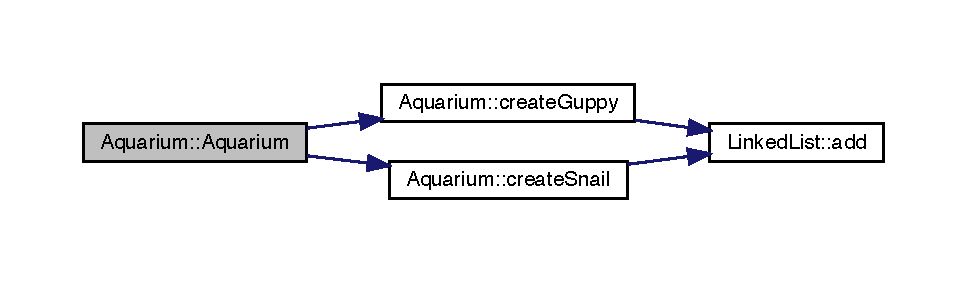
\includegraphics[width=350pt]{class_aquarium_abd216182838b8edad8626a580e6e99e1_cgraph}
\end{center}
\end{figure}
\mbox{\Hypertarget{class_aquarium_a40f31f27104d48e4f558d40059f4a590}\label{class_aquarium_a40f31f27104d48e4f558d40059f4a590}} 
\index{Aquarium@{Aquarium}!````~Aquarium@{$\sim$\+Aquarium}}
\index{````~Aquarium@{$\sim$\+Aquarium}!Aquarium@{Aquarium}}
\subsubsection{\texorpdfstring{$\sim$\+Aquarium()}{~Aquarium()}}
{\footnotesize\ttfamily Aquarium\+::$\sim$\+Aquarium (\begin{DoxyParamCaption}{ }\end{DoxyParamCaption})}



A destructor. 

Destructs the \mbox{\hyperlink{class_aquarium}{Aquarium}} object. 

\subsection{Member Function Documentation}
\mbox{\Hypertarget{class_aquarium_aec1e8fb9d89399012733c747ec9e80ff}\label{class_aquarium_aec1e8fb9d89399012733c747ec9e80ff}} 
\index{Aquarium@{Aquarium}!create\+Coin@{create\+Coin}}
\index{create\+Coin@{create\+Coin}!Aquarium@{Aquarium}}
\subsubsection{\texorpdfstring{create\+Coin()}{createCoin()}}
{\footnotesize\ttfamily void Aquarium\+::create\+Coin (\begin{DoxyParamCaption}\item[{double}]{x,  }\item[{double}]{y,  }\item[{int}]{value }\end{DoxyParamCaption})}



Create \mbox{\hyperlink{class_coin}{Coin}}. 

Creates a new \mbox{\hyperlink{class_coin}{Coin}} and adds it to content\+\_\+coin list. 
\begin{DoxyParams}{Parameters}
{\em double} & x x-\/axis position of the newly created \mbox{\hyperlink{class_coin}{Coin}}. \\
\hline
{\em double} & y y-\/axis position of the newly created \mbox{\hyperlink{class_coin}{Coin}}. \\
\hline
{\em int} & value the value of the \mbox{\hyperlink{class_coin}{Coin}} \\
\hline
\end{DoxyParams}
Here is the call graph for this function\+:\nopagebreak
\begin{figure}[H]
\begin{center}
\leavevmode
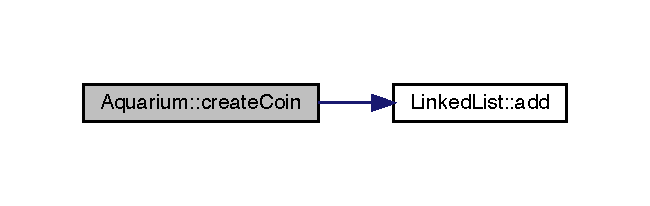
\includegraphics[width=312pt]{class_aquarium_aec1e8fb9d89399012733c747ec9e80ff_cgraph}
\end{center}
\end{figure}
Here is the caller graph for this function\+:
\nopagebreak
\begin{figure}[H]
\begin{center}
\leavevmode
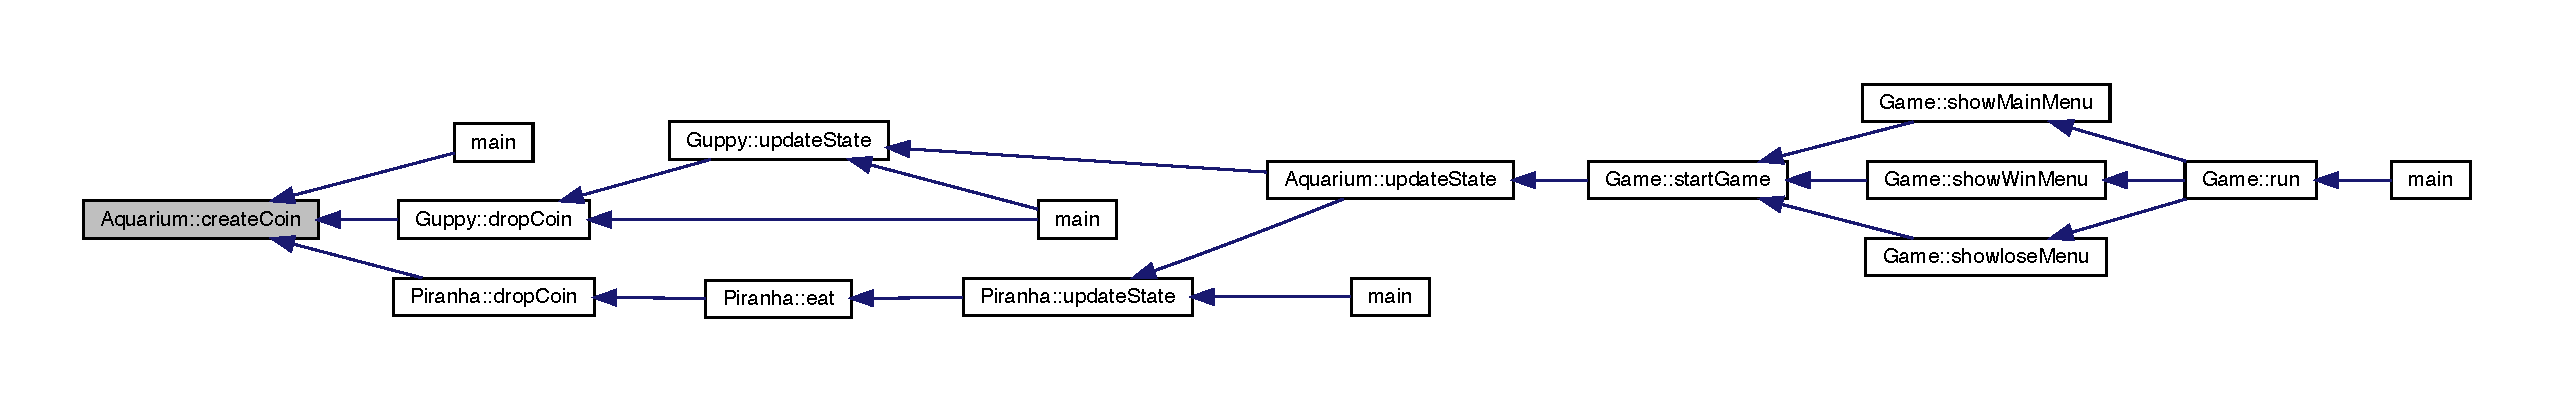
\includegraphics[width=350pt]{class_aquarium_aec1e8fb9d89399012733c747ec9e80ff_icgraph}
\end{center}
\end{figure}
\mbox{\Hypertarget{class_aquarium_a44ab0beff51d6607e0f590270d9066b5}\label{class_aquarium_a44ab0beff51d6607e0f590270d9066b5}} 
\index{Aquarium@{Aquarium}!create\+Guppy@{create\+Guppy}}
\index{create\+Guppy@{create\+Guppy}!Aquarium@{Aquarium}}
\subsubsection{\texorpdfstring{create\+Guppy()}{createGuppy()}}
{\footnotesize\ttfamily void Aquarium\+::create\+Guppy (\begin{DoxyParamCaption}{ }\end{DoxyParamCaption})}



Create \mbox{\hyperlink{class_guppy}{Guppy}}. 

Creates a new \mbox{\hyperlink{class_guppy}{Guppy}} and adds it to content\+\_\+guppy list. Here is the call graph for this function\+:\nopagebreak
\begin{figure}[H]
\begin{center}
\leavevmode
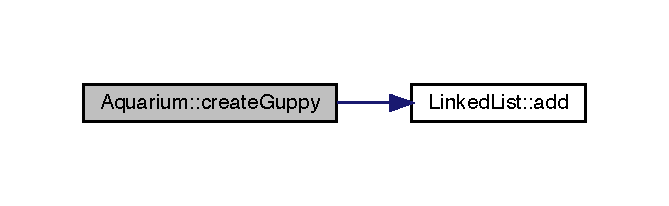
\includegraphics[width=321pt]{class_aquarium_a44ab0beff51d6607e0f590270d9066b5_cgraph}
\end{center}
\end{figure}
Here is the caller graph for this function\+:
\nopagebreak
\begin{figure}[H]
\begin{center}
\leavevmode
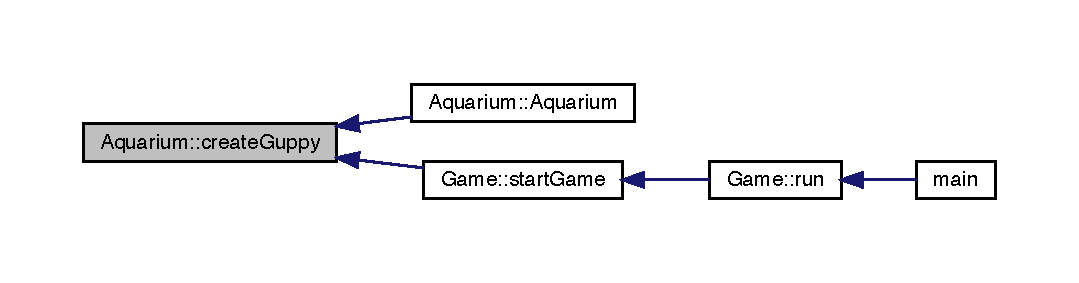
\includegraphics[width=350pt]{class_aquarium_a44ab0beff51d6607e0f590270d9066b5_icgraph}
\end{center}
\end{figure}
\mbox{\Hypertarget{class_aquarium_a049ffa77e7bbb68ac031a098c4e635e7}\label{class_aquarium_a049ffa77e7bbb68ac031a098c4e635e7}} 
\index{Aquarium@{Aquarium}!create\+Pellet@{create\+Pellet}}
\index{create\+Pellet@{create\+Pellet}!Aquarium@{Aquarium}}
\subsubsection{\texorpdfstring{create\+Pellet()}{createPellet()}}
{\footnotesize\ttfamily void Aquarium\+::create\+Pellet (\begin{DoxyParamCaption}\item[{double}]{x,  }\item[{double}]{y }\end{DoxyParamCaption})}



Create \mbox{\hyperlink{class_pellet}{Pellet}}. 

Creates a new \mbox{\hyperlink{class_pellet}{Pellet}} and adds it to content\+\_\+pellet list. 
\begin{DoxyParams}{Parameters}
{\em double} & x x-\/axis position of the newly created \mbox{\hyperlink{class_pellet}{Pellet}}. \\
\hline
{\em double} & y y-\/axis position of the newly created \mbox{\hyperlink{class_pellet}{Pellet}}. \\
\hline
\end{DoxyParams}
Here is the call graph for this function\+:\nopagebreak
\begin{figure}[H]
\begin{center}
\leavevmode
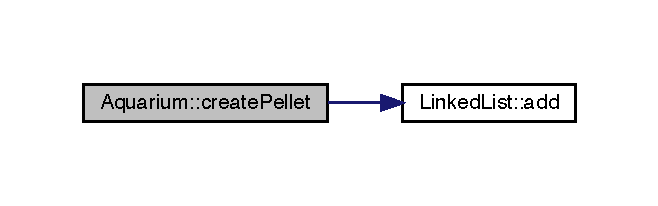
\includegraphics[width=316pt]{class_aquarium_a049ffa77e7bbb68ac031a098c4e635e7_cgraph}
\end{center}
\end{figure}
Here is the caller graph for this function\+:
\nopagebreak
\begin{figure}[H]
\begin{center}
\leavevmode
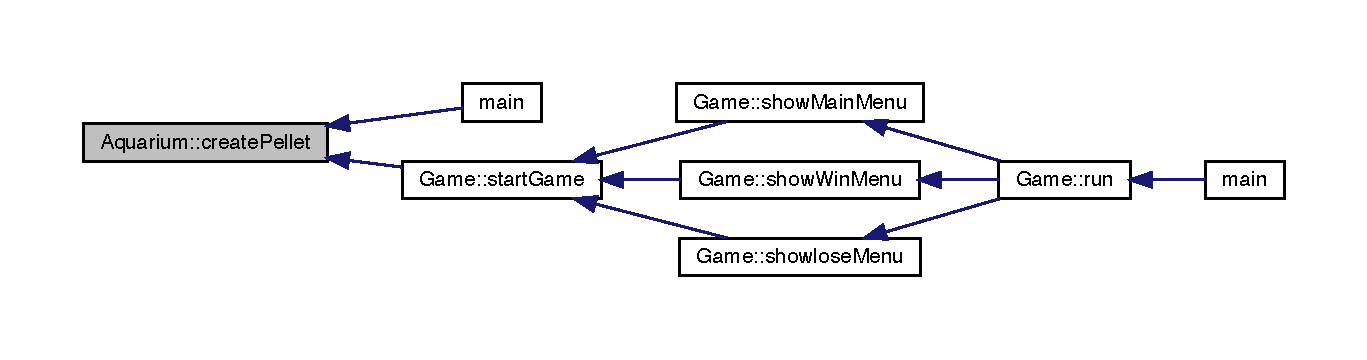
\includegraphics[width=350pt]{class_aquarium_a049ffa77e7bbb68ac031a098c4e635e7_icgraph}
\end{center}
\end{figure}
\mbox{\Hypertarget{class_aquarium_a416b16bc7c252260b9cbe053a6e5a76c}\label{class_aquarium_a416b16bc7c252260b9cbe053a6e5a76c}} 
\index{Aquarium@{Aquarium}!create\+Piranha@{create\+Piranha}}
\index{create\+Piranha@{create\+Piranha}!Aquarium@{Aquarium}}
\subsubsection{\texorpdfstring{create\+Piranha()}{createPiranha()}}
{\footnotesize\ttfamily void Aquarium\+::create\+Piranha (\begin{DoxyParamCaption}{ }\end{DoxyParamCaption})}



Create \mbox{\hyperlink{class_piranha}{Piranha}}. 

Creates a new \mbox{\hyperlink{class_piranha}{Piranha}} and adds it to content\+\_\+piranha list. Here is the call graph for this function\+:\nopagebreak
\begin{figure}[H]
\begin{center}
\leavevmode
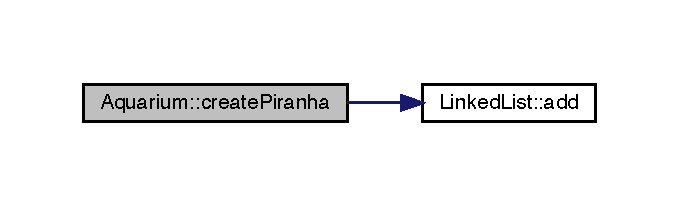
\includegraphics[width=326pt]{class_aquarium_a416b16bc7c252260b9cbe053a6e5a76c_cgraph}
\end{center}
\end{figure}
Here is the caller graph for this function\+:
\nopagebreak
\begin{figure}[H]
\begin{center}
\leavevmode
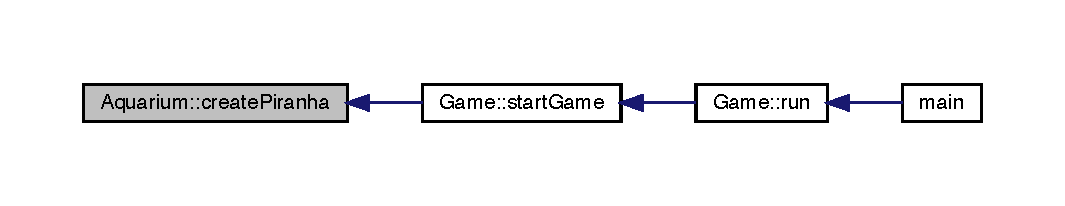
\includegraphics[width=350pt]{class_aquarium_a416b16bc7c252260b9cbe053a6e5a76c_icgraph}
\end{center}
\end{figure}
\mbox{\Hypertarget{class_aquarium_ae631c3fd8587b1889ffea4e0ade6359e}\label{class_aquarium_ae631c3fd8587b1889ffea4e0ade6359e}} 
\index{Aquarium@{Aquarium}!create\+Snail@{create\+Snail}}
\index{create\+Snail@{create\+Snail}!Aquarium@{Aquarium}}
\subsubsection{\texorpdfstring{create\+Snail()}{createSnail()}}
{\footnotesize\ttfamily void Aquarium\+::create\+Snail (\begin{DoxyParamCaption}{ }\end{DoxyParamCaption})}



Create \mbox{\hyperlink{class_snail}{Snail}}. 

Creates a new \mbox{\hyperlink{class_snail}{Snail}} and adds it to content\+\_\+snail list. Here is the call graph for this function\+:\nopagebreak
\begin{figure}[H]
\begin{center}
\leavevmode
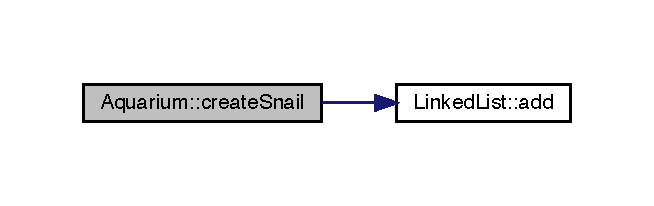
\includegraphics[width=314pt]{class_aquarium_ae631c3fd8587b1889ffea4e0ade6359e_cgraph}
\end{center}
\end{figure}
Here is the caller graph for this function\+:
\nopagebreak
\begin{figure}[H]
\begin{center}
\leavevmode
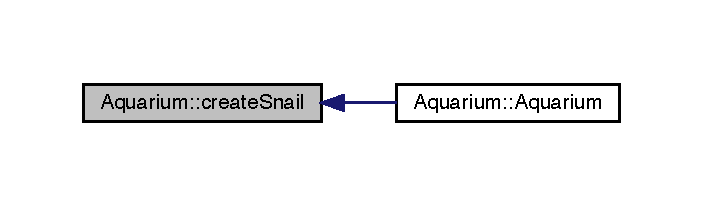
\includegraphics[width=350pt]{class_aquarium_ae631c3fd8587b1889ffea4e0ade6359e_icgraph}
\end{center}
\end{figure}
\mbox{\Hypertarget{class_aquarium_a187e59dd6efd62b577e97b8e00237c77}\label{class_aquarium_a187e59dd6efd62b577e97b8e00237c77}} 
\index{Aquarium@{Aquarium}!delete\+Coin@{delete\+Coin}}
\index{delete\+Coin@{delete\+Coin}!Aquarium@{Aquarium}}
\subsubsection{\texorpdfstring{delete\+Coin()}{deleteCoin()}}
{\footnotesize\ttfamily void Aquarium\+::delete\+Coin (\begin{DoxyParamCaption}\item[{\mbox{\hyperlink{class_coin}{Coin}} $\ast$}]{c }\end{DoxyParamCaption})}



Delete \mbox{\hyperlink{class_coin}{Coin}}. 

Deletes a \mbox{\hyperlink{class_coin}{Coin}} and removes it from content\+\_\+coin list. 
\begin{DoxyParams}{Parameters}
{\em \mbox{\hyperlink{class_coin}{Coin}}} & $\ast$c Pointer to the \mbox{\hyperlink{class_coin}{Coin}}. \\
\hline
\end{DoxyParams}
Here is the call graph for this function\+:\nopagebreak
\begin{figure}[H]
\begin{center}
\leavevmode
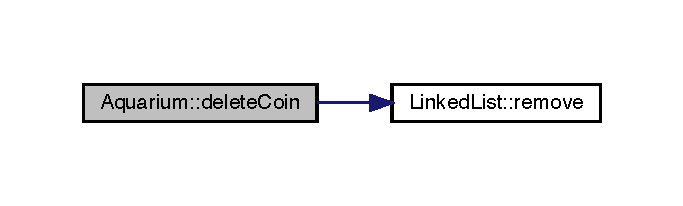
\includegraphics[width=328pt]{class_aquarium_a187e59dd6efd62b577e97b8e00237c77_cgraph}
\end{center}
\end{figure}
Here is the caller graph for this function\+:
\nopagebreak
\begin{figure}[H]
\begin{center}
\leavevmode
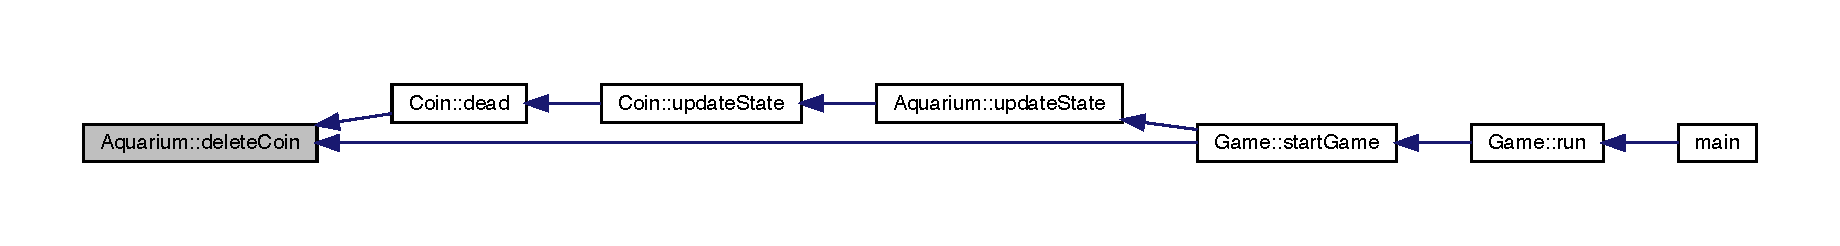
\includegraphics[width=350pt]{class_aquarium_a187e59dd6efd62b577e97b8e00237c77_icgraph}
\end{center}
\end{figure}
\mbox{\Hypertarget{class_aquarium_ae2372aef40d9474573833262b6062eb2}\label{class_aquarium_ae2372aef40d9474573833262b6062eb2}} 
\index{Aquarium@{Aquarium}!delete\+Guppy@{delete\+Guppy}}
\index{delete\+Guppy@{delete\+Guppy}!Aquarium@{Aquarium}}
\subsubsection{\texorpdfstring{delete\+Guppy()}{deleteGuppy()}}
{\footnotesize\ttfamily void Aquarium\+::delete\+Guppy (\begin{DoxyParamCaption}\item[{\mbox{\hyperlink{class_guppy}{Guppy}} $\ast$}]{g }\end{DoxyParamCaption})}



Delete \mbox{\hyperlink{class_guppy}{Guppy}}. 

Deletes a \mbox{\hyperlink{class_guppy}{Guppy}} and removes it from content\+\_\+guppy list. 
\begin{DoxyParams}{Parameters}
{\em \mbox{\hyperlink{class_guppy}{Guppy}}} & $\ast$g Pointer to the \mbox{\hyperlink{class_guppy}{Guppy}}. \\
\hline
\end{DoxyParams}
Here is the call graph for this function\+:\nopagebreak
\begin{figure}[H]
\begin{center}
\leavevmode
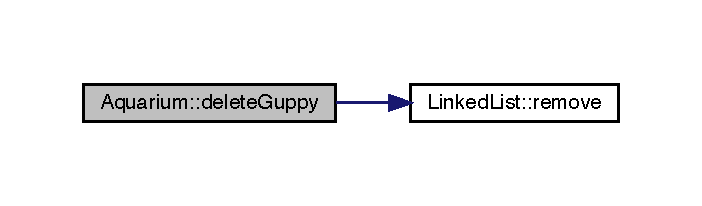
\includegraphics[width=337pt]{class_aquarium_ae2372aef40d9474573833262b6062eb2_cgraph}
\end{center}
\end{figure}
Here is the caller graph for this function\+:
\nopagebreak
\begin{figure}[H]
\begin{center}
\leavevmode
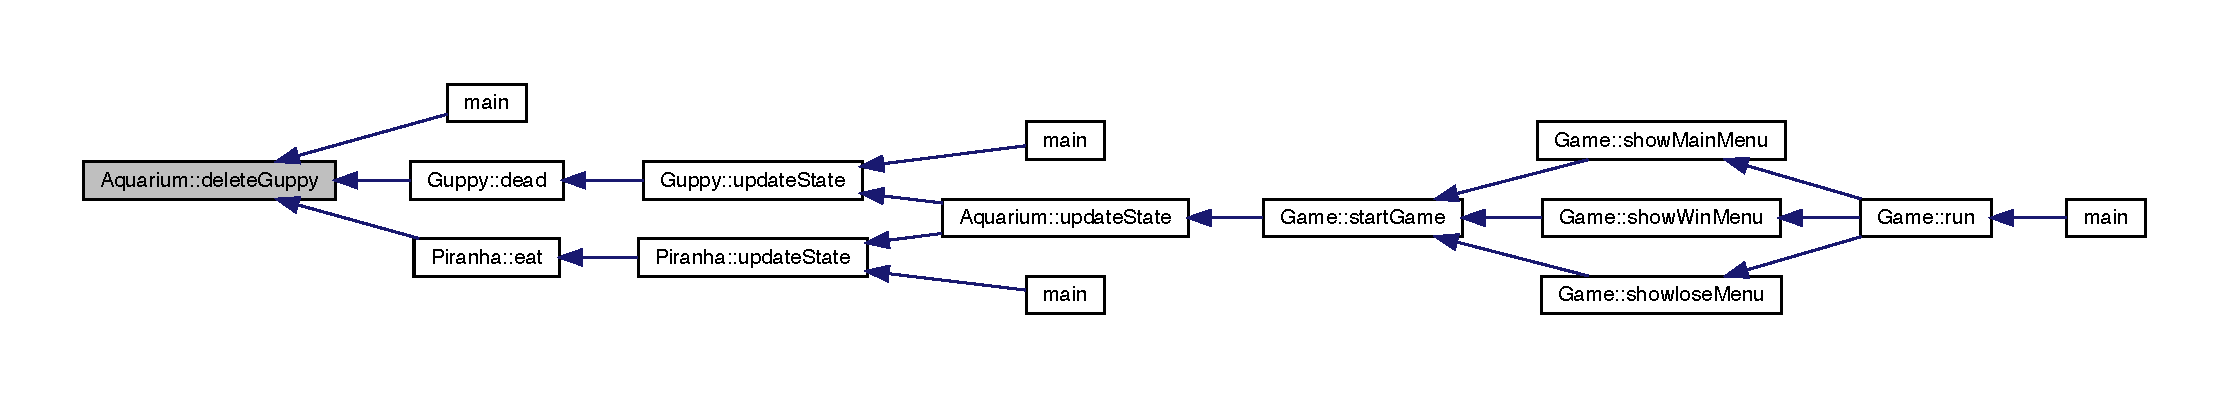
\includegraphics[width=350pt]{class_aquarium_ae2372aef40d9474573833262b6062eb2_icgraph}
\end{center}
\end{figure}
\mbox{\Hypertarget{class_aquarium_a61329fb56bcb5af2e06fc62568456f1b}\label{class_aquarium_a61329fb56bcb5af2e06fc62568456f1b}} 
\index{Aquarium@{Aquarium}!delete\+Pellet@{delete\+Pellet}}
\index{delete\+Pellet@{delete\+Pellet}!Aquarium@{Aquarium}}
\subsubsection{\texorpdfstring{delete\+Pellet()}{deletePellet()}}
{\footnotesize\ttfamily void Aquarium\+::delete\+Pellet (\begin{DoxyParamCaption}\item[{\mbox{\hyperlink{class_pellet}{Pellet}} $\ast$}]{p }\end{DoxyParamCaption})}



Delete \mbox{\hyperlink{class_pellet}{Pellet}}. 

Deletes a \mbox{\hyperlink{class_pellet}{Pellet}} and removes it from content\+\_\+pellet list. 
\begin{DoxyParams}{Parameters}
{\em \mbox{\hyperlink{class_pellet}{Pellet}}} & $\ast$p Pointer to the \mbox{\hyperlink{class_pellet}{Pellet}}. \\
\hline
\end{DoxyParams}
Here is the call graph for this function\+:\nopagebreak
\begin{figure}[H]
\begin{center}
\leavevmode
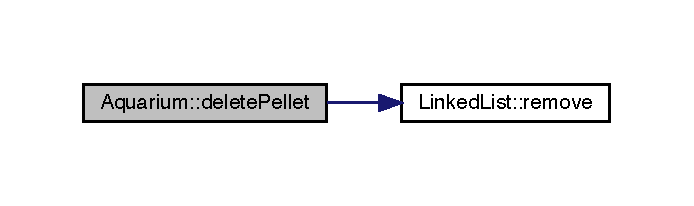
\includegraphics[width=333pt]{class_aquarium_a61329fb56bcb5af2e06fc62568456f1b_cgraph}
\end{center}
\end{figure}
Here is the caller graph for this function\+:
\nopagebreak
\begin{figure}[H]
\begin{center}
\leavevmode
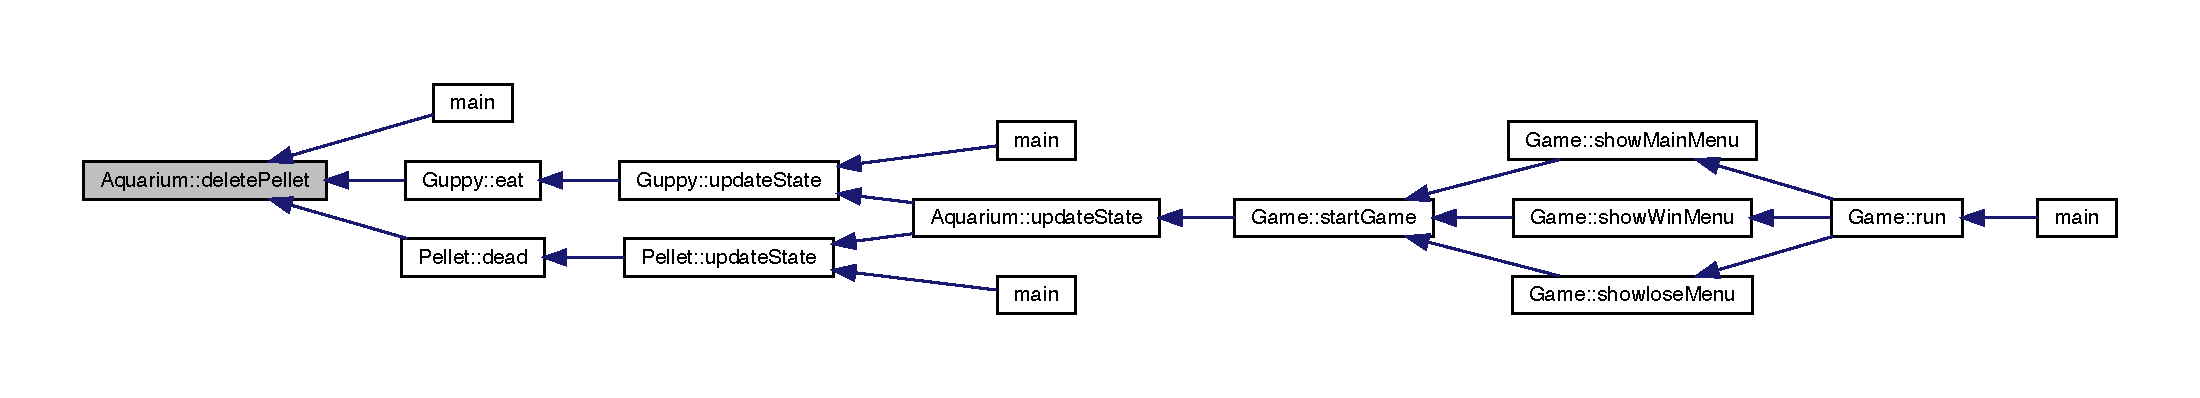
\includegraphics[width=350pt]{class_aquarium_a61329fb56bcb5af2e06fc62568456f1b_icgraph}
\end{center}
\end{figure}
\mbox{\Hypertarget{class_aquarium_a86cec76f7e0cbbdff79d5cef1e6e7f84}\label{class_aquarium_a86cec76f7e0cbbdff79d5cef1e6e7f84}} 
\index{Aquarium@{Aquarium}!delete\+Piranha@{delete\+Piranha}}
\index{delete\+Piranha@{delete\+Piranha}!Aquarium@{Aquarium}}
\subsubsection{\texorpdfstring{delete\+Piranha()}{deletePiranha()}}
{\footnotesize\ttfamily void Aquarium\+::delete\+Piranha (\begin{DoxyParamCaption}\item[{\mbox{\hyperlink{class_piranha}{Piranha}} $\ast$}]{p }\end{DoxyParamCaption})}



Delete \mbox{\hyperlink{class_piranha}{Piranha}}. 

Deletes a \mbox{\hyperlink{class_piranha}{Piranha}} and removes it from content\+\_\+piranha list. 
\begin{DoxyParams}{Parameters}
{\em \mbox{\hyperlink{class_piranha}{Piranha}}} & $\ast$p Pointer to the \mbox{\hyperlink{class_piranha}{Piranha}}. \\
\hline
\end{DoxyParams}
Here is the call graph for this function\+:\nopagebreak
\begin{figure}[H]
\begin{center}
\leavevmode
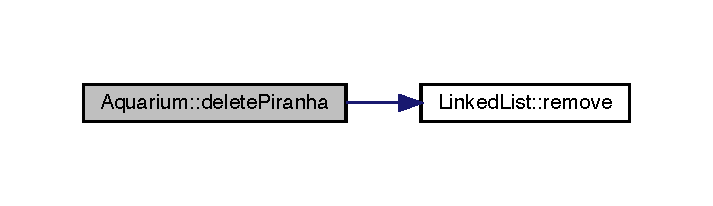
\includegraphics[width=342pt]{class_aquarium_a86cec76f7e0cbbdff79d5cef1e6e7f84_cgraph}
\end{center}
\end{figure}
Here is the caller graph for this function\+:
\nopagebreak
\begin{figure}[H]
\begin{center}
\leavevmode
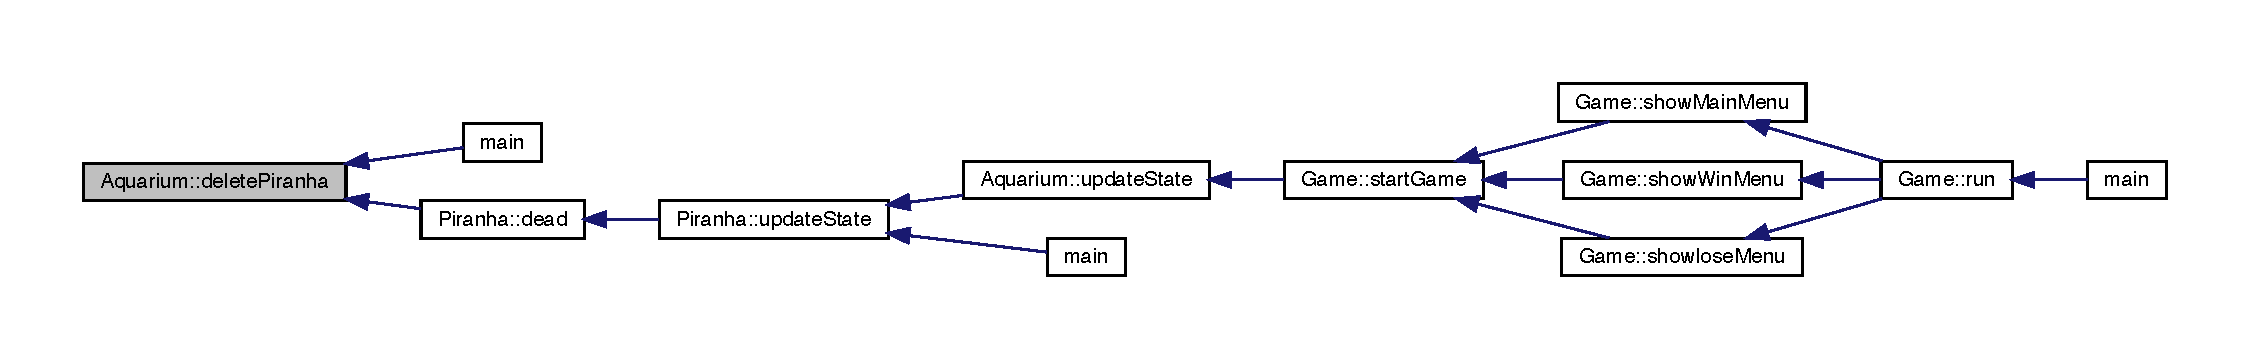
\includegraphics[width=350pt]{class_aquarium_a86cec76f7e0cbbdff79d5cef1e6e7f84_icgraph}
\end{center}
\end{figure}
\mbox{\Hypertarget{class_aquarium_a08048866266aabb12b8cc82bac042c18}\label{class_aquarium_a08048866266aabb12b8cc82bac042c18}} 
\index{Aquarium@{Aquarium}!delete\+Snail@{delete\+Snail}}
\index{delete\+Snail@{delete\+Snail}!Aquarium@{Aquarium}}
\subsubsection{\texorpdfstring{delete\+Snail()}{deleteSnail()}}
{\footnotesize\ttfamily void Aquarium\+::delete\+Snail (\begin{DoxyParamCaption}\item[{\mbox{\hyperlink{class_snail}{Snail}} $\ast$}]{s }\end{DoxyParamCaption})}



Delete \mbox{\hyperlink{class_snail}{Snail}}. 

Deletes a \mbox{\hyperlink{class_snail}{Snail}} and removes it from content\+\_\+snail list. 
\begin{DoxyParams}{Parameters}
{\em \mbox{\hyperlink{class_snail}{Snail}}} & $\ast$s Pointer to the \mbox{\hyperlink{class_snail}{Snail}}. \\
\hline
\end{DoxyParams}
Here is the call graph for this function\+:\nopagebreak
\begin{figure}[H]
\begin{center}
\leavevmode
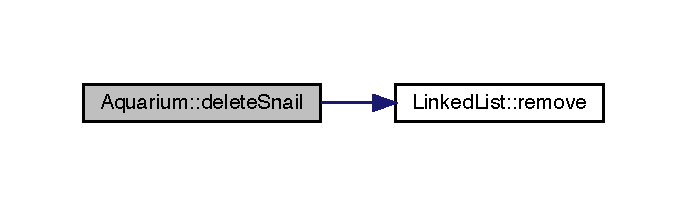
\includegraphics[width=330pt]{class_aquarium_a08048866266aabb12b8cc82bac042c18_cgraph}
\end{center}
\end{figure}
Here is the caller graph for this function\+:\nopagebreak
\begin{figure}[H]
\begin{center}
\leavevmode
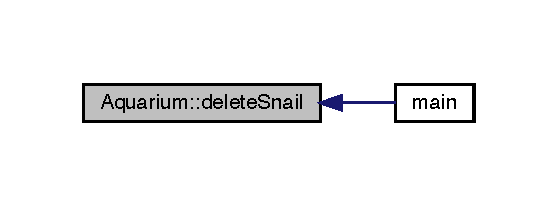
\includegraphics[width=268pt]{class_aquarium_a08048866266aabb12b8cc82bac042c18_icgraph}
\end{center}
\end{figure}
\mbox{\Hypertarget{class_aquarium_a3b3592004ace881a5e11d19a8dc127e4}\label{class_aquarium_a3b3592004ace881a5e11d19a8dc127e4}} 
\index{Aquarium@{Aquarium}!get\+Coin\+List@{get\+Coin\+List}}
\index{get\+Coin\+List@{get\+Coin\+List}!Aquarium@{Aquarium}}
\subsubsection{\texorpdfstring{get\+Coin\+List()}{getCoinList()}}
{\footnotesize\ttfamily \mbox{\hyperlink{class_linked_list}{Linked\+List}}$<$ \mbox{\hyperlink{class_coin}{Coin}} $\ast$ $>$ \& Aquarium\+::get\+Coin\+List (\begin{DoxyParamCaption}{ }\end{DoxyParamCaption})}



Getter for content\+\_\+coin list. 

\begin{DoxyReturn}{Returns}
Linked\+List$<$\+Coin $\ast$$>$\& list of all \mbox{\hyperlink{class_coin}{Coin}} 
\end{DoxyReturn}
Here is the caller graph for this function\+:
\nopagebreak
\begin{figure}[H]
\begin{center}
\leavevmode
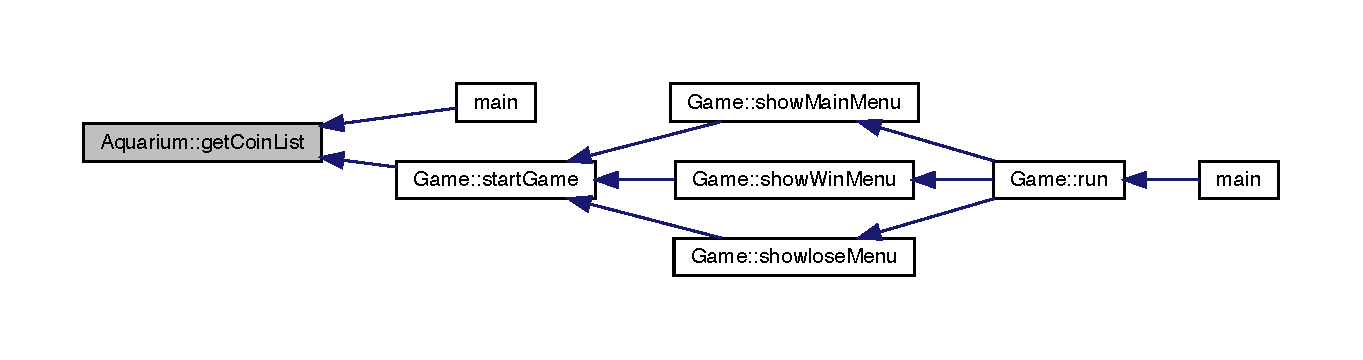
\includegraphics[width=350pt]{class_aquarium_a3b3592004ace881a5e11d19a8dc127e4_icgraph}
\end{center}
\end{figure}
\mbox{\Hypertarget{class_aquarium_aae7158daf192a78ffaf165285386221f}\label{class_aquarium_aae7158daf192a78ffaf165285386221f}} 
\index{Aquarium@{Aquarium}!get\+Curr\+Time@{get\+Curr\+Time}}
\index{get\+Curr\+Time@{get\+Curr\+Time}!Aquarium@{Aquarium}}
\subsubsection{\texorpdfstring{get\+Curr\+Time()}{getCurrTime()}}
{\footnotesize\ttfamily double Aquarium\+::get\+Curr\+Time (\begin{DoxyParamCaption}{ }\end{DoxyParamCaption})}



Getter for curr\+\_\+time. 

\begin{DoxyReturn}{Returns}
double curr\+\_\+time 
\end{DoxyReturn}
Here is the caller graph for this function\+:
\nopagebreak
\begin{figure}[H]
\begin{center}
\leavevmode
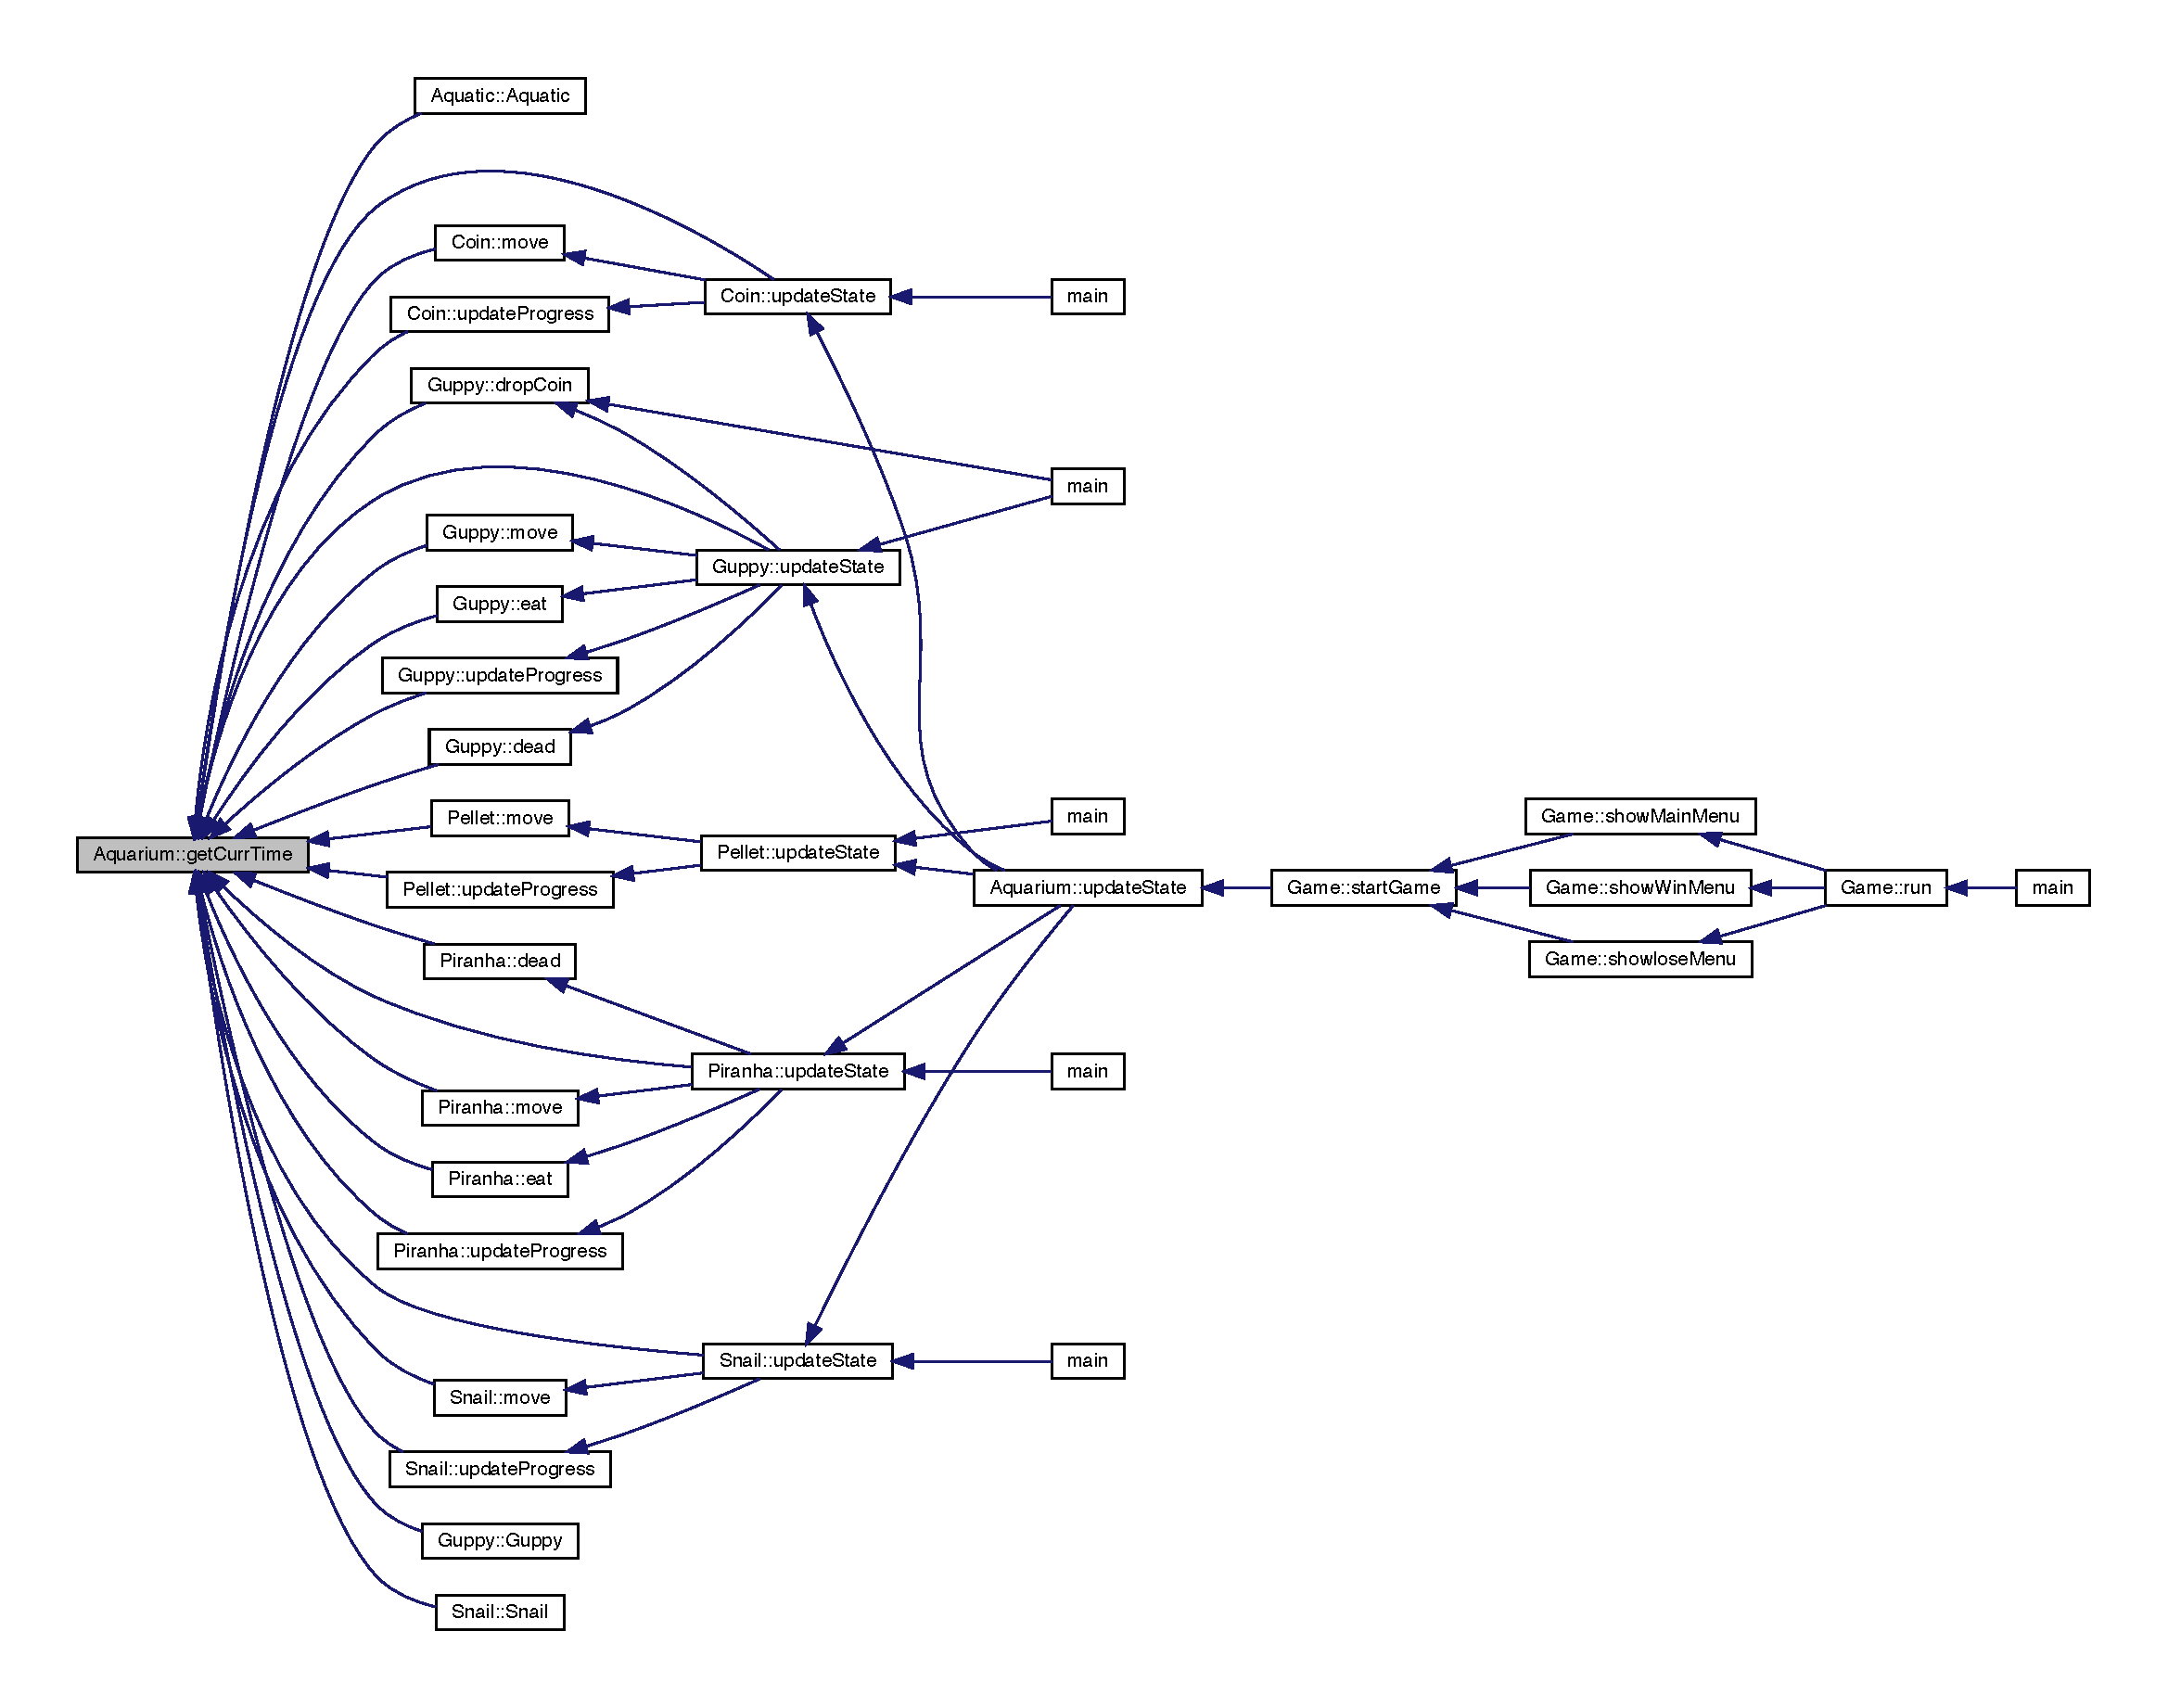
\includegraphics[width=350pt]{class_aquarium_aae7158daf192a78ffaf165285386221f_icgraph}
\end{center}
\end{figure}
\mbox{\Hypertarget{class_aquarium_a3244b33f404c2887f04342754f17f4ee}\label{class_aquarium_a3244b33f404c2887f04342754f17f4ee}} 
\index{Aquarium@{Aquarium}!get\+Guppy\+List@{get\+Guppy\+List}}
\index{get\+Guppy\+List@{get\+Guppy\+List}!Aquarium@{Aquarium}}
\subsubsection{\texorpdfstring{get\+Guppy\+List()}{getGuppyList()}}
{\footnotesize\ttfamily \mbox{\hyperlink{class_linked_list}{Linked\+List}}$<$ \mbox{\hyperlink{class_guppy}{Guppy}} $\ast$ $>$ \& Aquarium\+::get\+Guppy\+List (\begin{DoxyParamCaption}{ }\end{DoxyParamCaption})}



Getter for content\+\_\+guppy list. 

\begin{DoxyReturn}{Returns}
Linked\+List$<$\+Guppy $\ast$$>$\& list of all \mbox{\hyperlink{class_guppy}{Guppy}} 
\end{DoxyReturn}
Here is the caller graph for this function\+:
\nopagebreak
\begin{figure}[H]
\begin{center}
\leavevmode
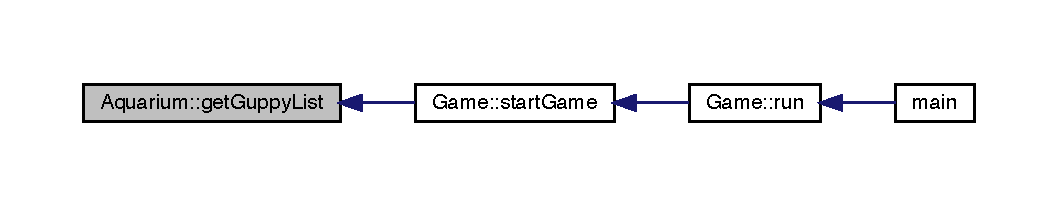
\includegraphics[width=350pt]{class_aquarium_a3244b33f404c2887f04342754f17f4ee_icgraph}
\end{center}
\end{figure}
\mbox{\Hypertarget{class_aquarium_a2d0eeed1f5776e13f0bbafc6844ce7a2}\label{class_aquarium_a2d0eeed1f5776e13f0bbafc6844ce7a2}} 
\index{Aquarium@{Aquarium}!get\+Pellet\+List@{get\+Pellet\+List}}
\index{get\+Pellet\+List@{get\+Pellet\+List}!Aquarium@{Aquarium}}
\subsubsection{\texorpdfstring{get\+Pellet\+List()}{getPelletList()}}
{\footnotesize\ttfamily \mbox{\hyperlink{class_linked_list}{Linked\+List}}$<$ \mbox{\hyperlink{class_pellet}{Pellet}} $\ast$ $>$ \& Aquarium\+::get\+Pellet\+List (\begin{DoxyParamCaption}{ }\end{DoxyParamCaption})}



Getter for content\+\_\+pellet list. 

\begin{DoxyReturn}{Returns}
Linked\+List$<$\+Pellet $\ast$$>$\& list of all \mbox{\hyperlink{class_pellet}{Pellet}} 
\end{DoxyReturn}
Here is the caller graph for this function\+:
\nopagebreak
\begin{figure}[H]
\begin{center}
\leavevmode
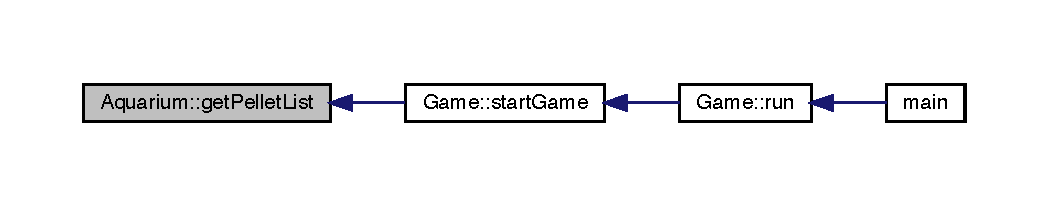
\includegraphics[width=350pt]{class_aquarium_a2d0eeed1f5776e13f0bbafc6844ce7a2_icgraph}
\end{center}
\end{figure}
\mbox{\Hypertarget{class_aquarium_a46c1697b25884c5a91f7a942ae5b3ba7}\label{class_aquarium_a46c1697b25884c5a91f7a942ae5b3ba7}} 
\index{Aquarium@{Aquarium}!get\+Piranha\+List@{get\+Piranha\+List}}
\index{get\+Piranha\+List@{get\+Piranha\+List}!Aquarium@{Aquarium}}
\subsubsection{\texorpdfstring{get\+Piranha\+List()}{getPiranhaList()}}
{\footnotesize\ttfamily \mbox{\hyperlink{class_linked_list}{Linked\+List}}$<$ \mbox{\hyperlink{class_piranha}{Piranha}} $\ast$ $>$ \& Aquarium\+::get\+Piranha\+List (\begin{DoxyParamCaption}{ }\end{DoxyParamCaption})}



Getter for content\+\_\+piranha list. 

\begin{DoxyReturn}{Returns}
Linked\+List$<$\+Piranha $\ast$$>$\& list of all \mbox{\hyperlink{class_piranha}{Piranha}} 
\end{DoxyReturn}
Here is the caller graph for this function\+:
\nopagebreak
\begin{figure}[H]
\begin{center}
\leavevmode
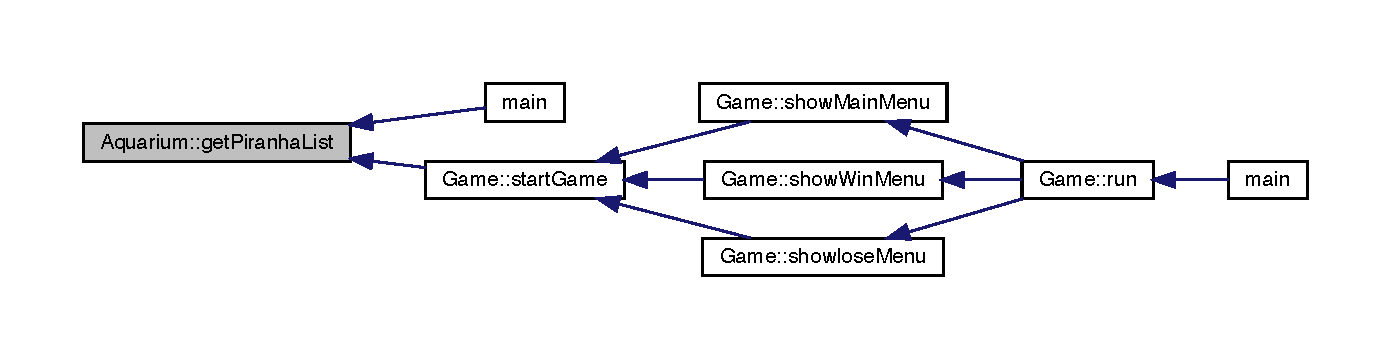
\includegraphics[width=350pt]{class_aquarium_a46c1697b25884c5a91f7a942ae5b3ba7_icgraph}
\end{center}
\end{figure}
\mbox{\Hypertarget{class_aquarium_a278a38d4cf238908c4e3e170ea66841f}\label{class_aquarium_a278a38d4cf238908c4e3e170ea66841f}} 
\index{Aquarium@{Aquarium}!get\+Snail\+List@{get\+Snail\+List}}
\index{get\+Snail\+List@{get\+Snail\+List}!Aquarium@{Aquarium}}
\subsubsection{\texorpdfstring{get\+Snail\+List()}{getSnailList()}}
{\footnotesize\ttfamily \mbox{\hyperlink{class_linked_list}{Linked\+List}}$<$ \mbox{\hyperlink{class_snail}{Snail}} $\ast$ $>$ \& Aquarium\+::get\+Snail\+List (\begin{DoxyParamCaption}{ }\end{DoxyParamCaption})}



Getter for content\+\_\+snail list. 

\begin{DoxyReturn}{Returns}
Linked\+List$<$\+Snail $\ast$$>$\& list of all \mbox{\hyperlink{class_snail}{Snail}} 
\end{DoxyReturn}
Here is the caller graph for this function\+:
\nopagebreak
\begin{figure}[H]
\begin{center}
\leavevmode
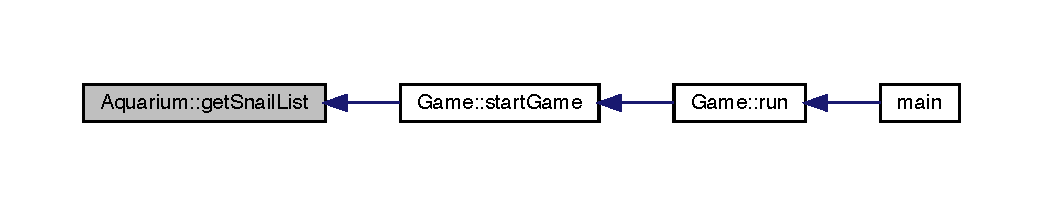
\includegraphics[width=350pt]{class_aquarium_a278a38d4cf238908c4e3e170ea66841f_icgraph}
\end{center}
\end{figure}
\mbox{\Hypertarget{class_aquarium_af0b5f88a7aaf71e817f809d7bee3e51e}\label{class_aquarium_af0b5f88a7aaf71e817f809d7bee3e51e}} 
\index{Aquarium@{Aquarium}!get\+X\+Max@{get\+X\+Max}}
\index{get\+X\+Max@{get\+X\+Max}!Aquarium@{Aquarium}}
\subsubsection{\texorpdfstring{get\+X\+Max()}{getXMax()}}
{\footnotesize\ttfamily double Aquarium\+::get\+X\+Max (\begin{DoxyParamCaption}{ }\end{DoxyParamCaption}) const}



Getter for x\+Max. 

\begin{DoxyReturn}{Returns}
double x\+Max 
\end{DoxyReturn}
Here is the caller graph for this function\+:
\nopagebreak
\begin{figure}[H]
\begin{center}
\leavevmode
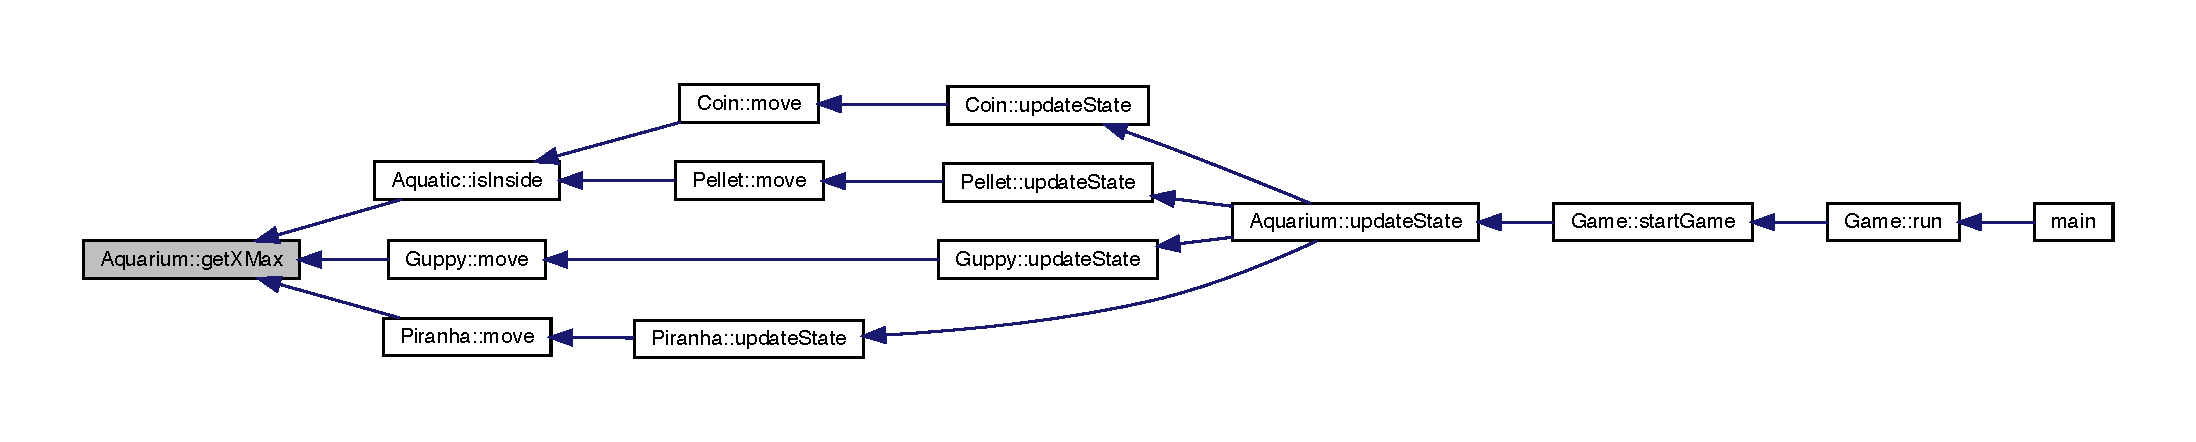
\includegraphics[width=350pt]{class_aquarium_af0b5f88a7aaf71e817f809d7bee3e51e_icgraph}
\end{center}
\end{figure}
\mbox{\Hypertarget{class_aquarium_a3e9e4b1bc86a90a8654bcc76e20e25f1}\label{class_aquarium_a3e9e4b1bc86a90a8654bcc76e20e25f1}} 
\index{Aquarium@{Aquarium}!get\+X\+Min@{get\+X\+Min}}
\index{get\+X\+Min@{get\+X\+Min}!Aquarium@{Aquarium}}
\subsubsection{\texorpdfstring{get\+X\+Min()}{getXMin()}}
{\footnotesize\ttfamily double Aquarium\+::get\+X\+Min (\begin{DoxyParamCaption}{ }\end{DoxyParamCaption}) const}



Getter for x\+Min. 

\begin{DoxyReturn}{Returns}
double x\+Min 
\end{DoxyReturn}
Here is the caller graph for this function\+:
\nopagebreak
\begin{figure}[H]
\begin{center}
\leavevmode
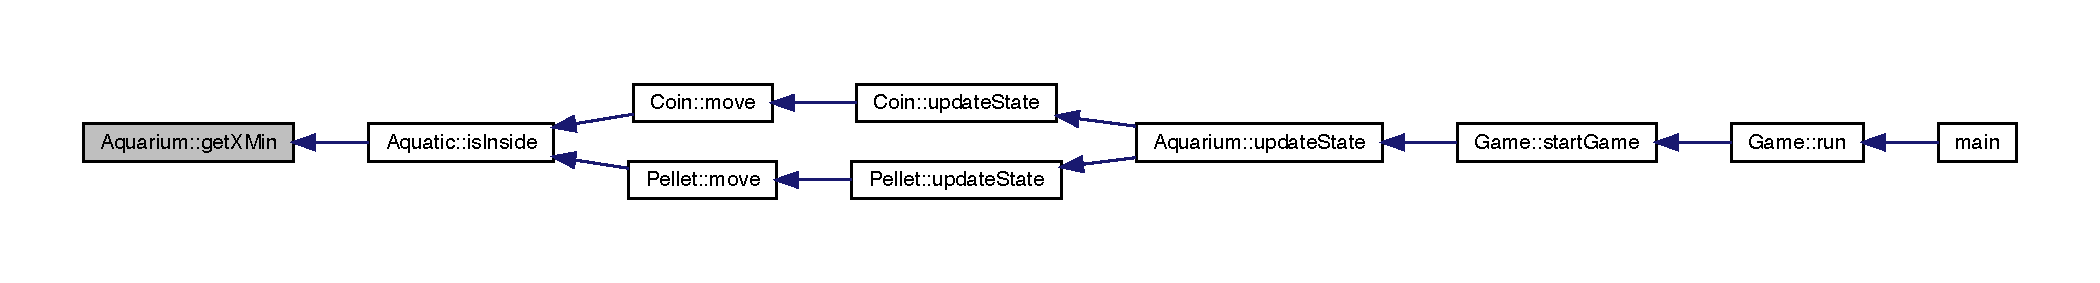
\includegraphics[width=350pt]{class_aquarium_a3e9e4b1bc86a90a8654bcc76e20e25f1_icgraph}
\end{center}
\end{figure}
\mbox{\Hypertarget{class_aquarium_a13893ca5240c99792040a7a64fd80bf5}\label{class_aquarium_a13893ca5240c99792040a7a64fd80bf5}} 
\index{Aquarium@{Aquarium}!get\+Y\+Max@{get\+Y\+Max}}
\index{get\+Y\+Max@{get\+Y\+Max}!Aquarium@{Aquarium}}
\subsubsection{\texorpdfstring{get\+Y\+Max()}{getYMax()}}
{\footnotesize\ttfamily double Aquarium\+::get\+Y\+Max (\begin{DoxyParamCaption}{ }\end{DoxyParamCaption}) const}



Getter for y\+Max. 

\begin{DoxyReturn}{Returns}
double y\+Max 
\end{DoxyReturn}
Here is the caller graph for this function\+:
\nopagebreak
\begin{figure}[H]
\begin{center}
\leavevmode
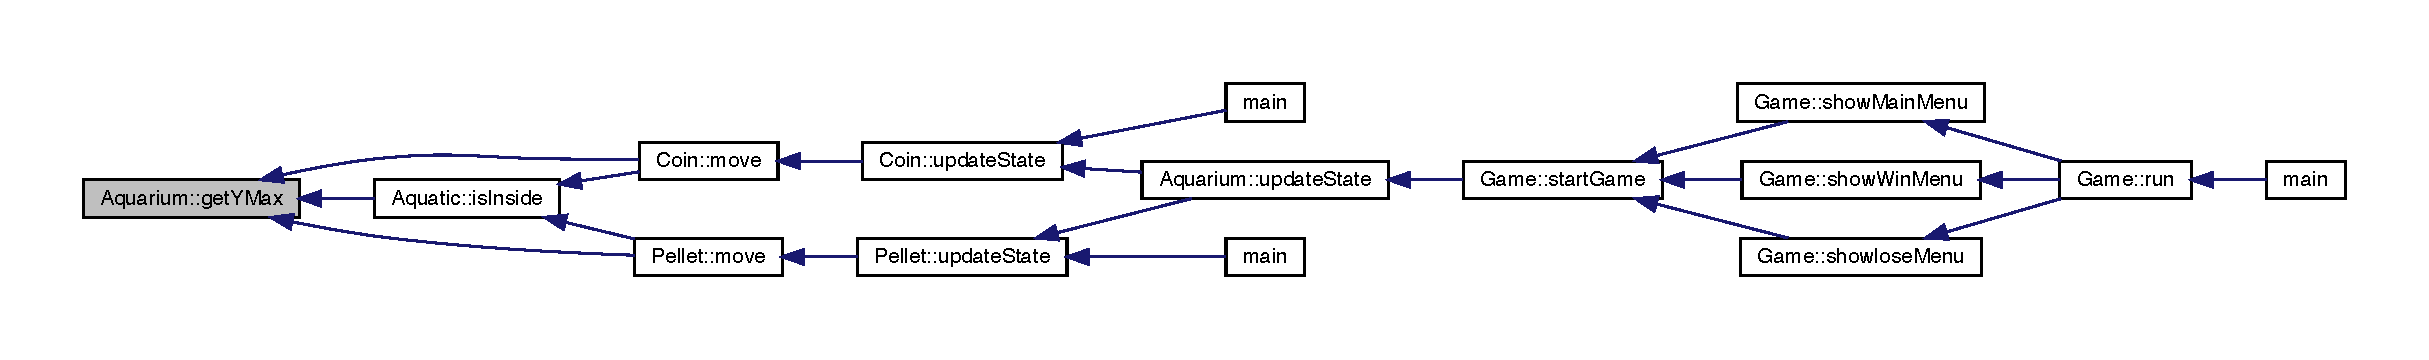
\includegraphics[width=350pt]{class_aquarium_a13893ca5240c99792040a7a64fd80bf5_icgraph}
\end{center}
\end{figure}
\mbox{\Hypertarget{class_aquarium_ad5ef328047a3a0815b32764f7114fbea}\label{class_aquarium_ad5ef328047a3a0815b32764f7114fbea}} 
\index{Aquarium@{Aquarium}!get\+Y\+Min@{get\+Y\+Min}}
\index{get\+Y\+Min@{get\+Y\+Min}!Aquarium@{Aquarium}}
\subsubsection{\texorpdfstring{get\+Y\+Min()}{getYMin()}}
{\footnotesize\ttfamily double Aquarium\+::get\+Y\+Min (\begin{DoxyParamCaption}{ }\end{DoxyParamCaption}) const}



Getter for y\+Min. 

\begin{DoxyReturn}{Returns}
double y\+Min 
\end{DoxyReturn}
Here is the caller graph for this function\+:
\nopagebreak
\begin{figure}[H]
\begin{center}
\leavevmode
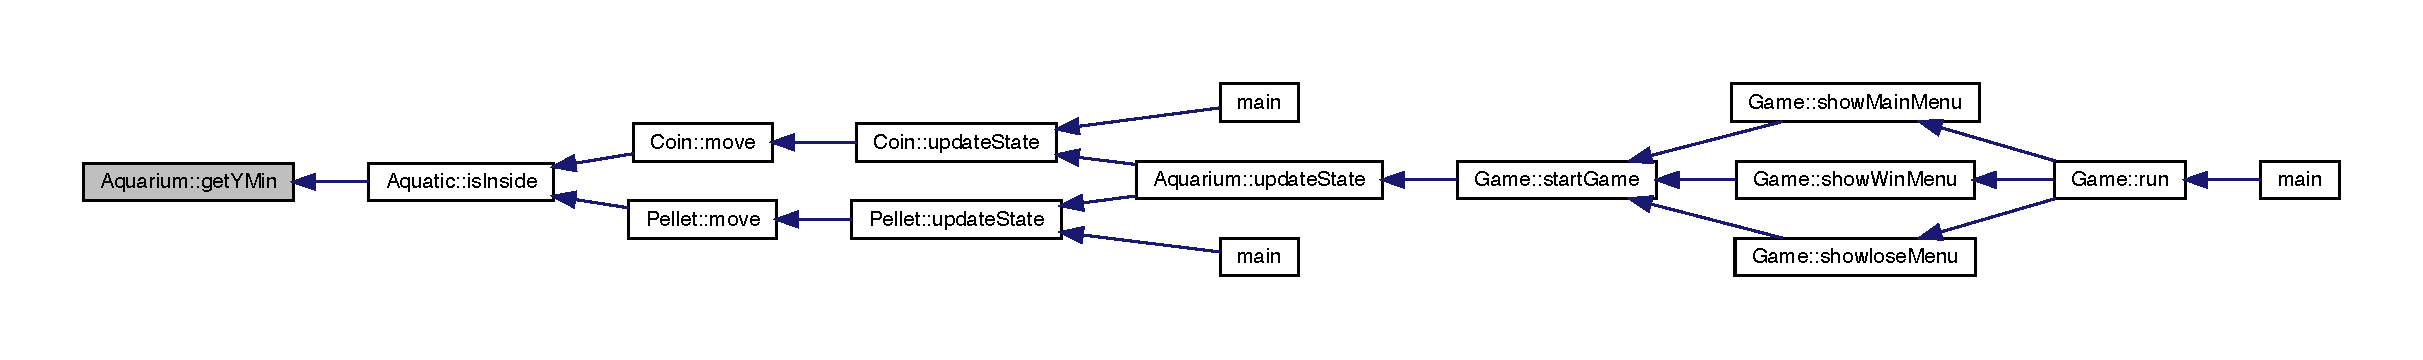
\includegraphics[width=350pt]{class_aquarium_ad5ef328047a3a0815b32764f7114fbea_icgraph}
\end{center}
\end{figure}
\mbox{\Hypertarget{class_aquarium_aa613d1ce40335c46aef9e4a8f44487ea}\label{class_aquarium_aa613d1ce40335c46aef9e4a8f44487ea}} 
\index{Aquarium@{Aquarium}!set\+Curr\+Time@{set\+Curr\+Time}}
\index{set\+Curr\+Time@{set\+Curr\+Time}!Aquarium@{Aquarium}}
\subsubsection{\texorpdfstring{set\+Curr\+Time()}{setCurrTime()}}
{\footnotesize\ttfamily void Aquarium\+::set\+Curr\+Time (\begin{DoxyParamCaption}\item[{double}]{t }\end{DoxyParamCaption})}



Setter for curr\+\_\+time. 


\begin{DoxyParams}{Parameters}
{\em double} & current time \\
\hline
\end{DoxyParams}
Here is the caller graph for this function\+:\nopagebreak
\begin{figure}[H]
\begin{center}
\leavevmode
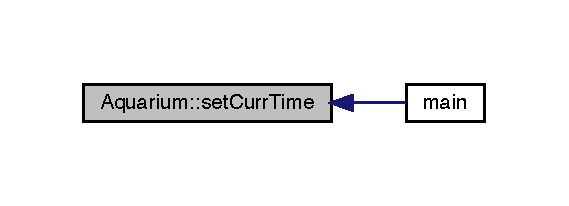
\includegraphics[width=273pt]{class_aquarium_aa613d1ce40335c46aef9e4a8f44487ea_icgraph}
\end{center}
\end{figure}
\mbox{\Hypertarget{class_aquarium_ac9fc0451e82c808d91a32a2e23e9f18e}\label{class_aquarium_ac9fc0451e82c808d91a32a2e23e9f18e}} 
\index{Aquarium@{Aquarium}!update\+State@{update\+State}}
\index{update\+State@{update\+State}!Aquarium@{Aquarium}}
\subsubsection{\texorpdfstring{update\+State()}{updateState()}}
{\footnotesize\ttfamily void Aquarium\+::update\+State (\begin{DoxyParamCaption}\item[{double}]{current\+\_\+time }\end{DoxyParamCaption})}



Updates all the aquarium object state. 


\begin{DoxyParams}{Parameters}
{\em double} & current time \\
\hline
\end{DoxyParams}
Here is the call graph for this function\+:\nopagebreak
\begin{figure}[H]
\begin{center}
\leavevmode
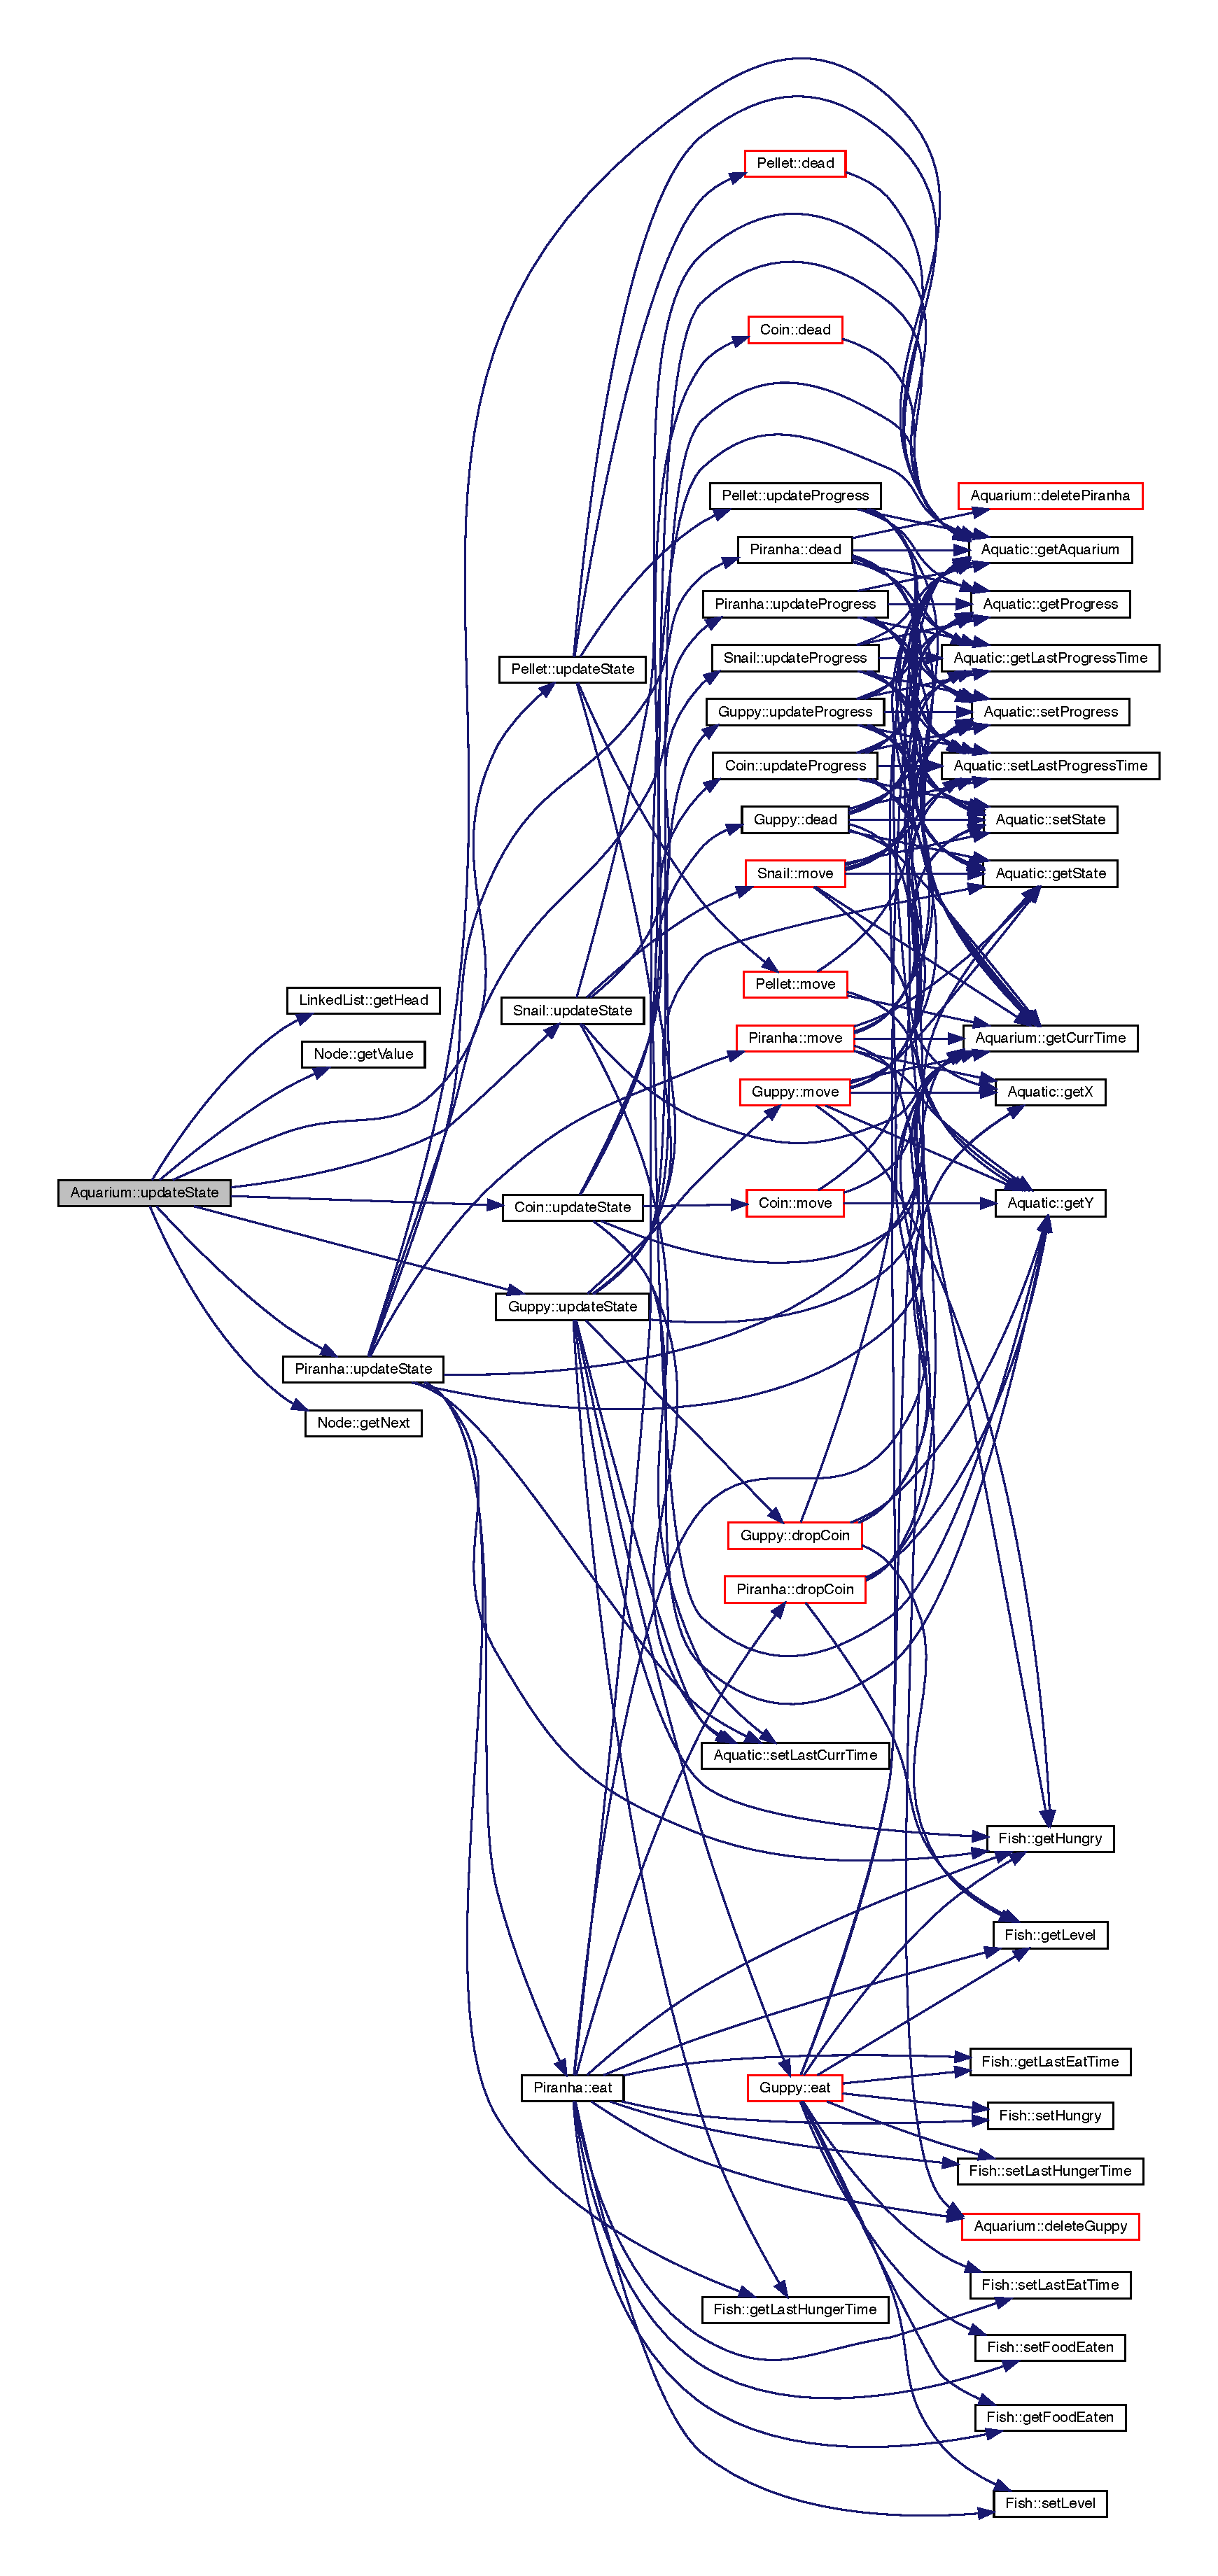
\includegraphics[height=550pt]{class_aquarium_ac9fc0451e82c808d91a32a2e23e9f18e_cgraph}
\end{center}
\end{figure}
Here is the caller graph for this function\+:
\nopagebreak
\begin{figure}[H]
\begin{center}
\leavevmode
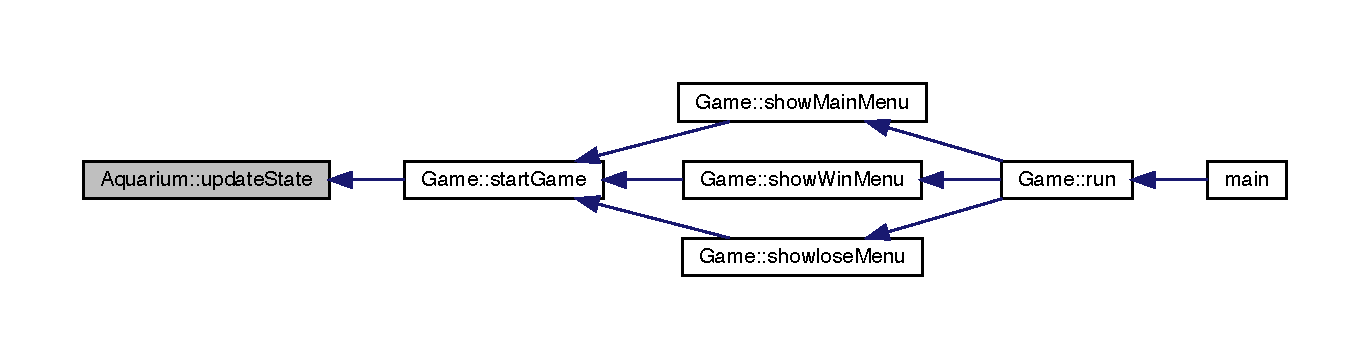
\includegraphics[width=350pt]{class_aquarium_ac9fc0451e82c808d91a32a2e23e9f18e_icgraph}
\end{center}
\end{figure}


The documentation for this class was generated from the following files\+:\begin{DoxyCompactItemize}
\item 
aquarium/\mbox{\hyperlink{_aquarium_8hpp}{Aquarium.\+hpp}}\item 
aquarium/\mbox{\hyperlink{_aquarium_8cpp}{Aquarium.\+cpp}}\end{DoxyCompactItemize}

\hypertarget{class_aquatic}{}\section{Aquatic Class Reference}
\label{class_aquatic}\index{Aquatic@{Aquatic}}


Abstract Class \mbox{\hyperlink{class_aquatic}{Aquatic}}. Represents all object in \mbox{\hyperlink{class_aquarium}{Aquarium}} such as \mbox{\hyperlink{class_piranha}{Piranha}}, \mbox{\hyperlink{class_guppy}{Guppy}}, \mbox{\hyperlink{class_snail}{Snail}}, \mbox{\hyperlink{class_pellet}{Pellet}}, and \mbox{\hyperlink{class_coin}{Coin}}.  




{\ttfamily \#include $<$Aquatic.\+hpp$>$}



Inheritance diagram for Aquatic\+:\nopagebreak
\begin{figure}[H]
\begin{center}
\leavevmode
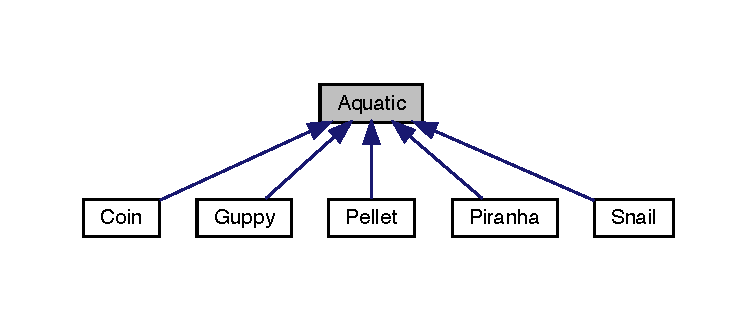
\includegraphics[width=350pt]{class_aquatic__inherit__graph}
\end{center}
\end{figure}
\subsection*{Public Member Functions}
\begin{DoxyCompactItemize}
\item 
\mbox{\hyperlink{class_aquatic_a302075a7330fcdf17dc0fc50ae62ada8}{Aquatic}} (\mbox{\hyperlink{class_aquarium}{Aquarium}} $\ast$aquarium)
\begin{DoxyCompactList}\small\item\em A constructor. \end{DoxyCompactList}\item 
\mbox{\hyperlink{class_aquatic_a01426b7729415006ede2c6238fc5849e}{Aquatic}} (double x, double y, double move\+\_\+speed, \mbox{\hyperlink{class_aquarium}{Aquarium}} $\ast$aquarium)
\begin{DoxyCompactList}\small\item\em A constructor. \end{DoxyCompactList}\item 
\mbox{\hyperlink{class_aquarium}{Aquarium}} $\ast$ \mbox{\hyperlink{class_aquatic_aa84812ff8347a11345b9c8231c1375cc}{get\+Aquarium}} ()
\begin{DoxyCompactList}\small\item\em Getter for aquarium. \end{DoxyCompactList}\item 
double \mbox{\hyperlink{class_aquatic_a4153178bfefdc57cbcd05fe44054dac9}{get\+Move\+Speed}} () const
\begin{DoxyCompactList}\small\item\em Getter for move\+\_\+speed. \end{DoxyCompactList}\item 
double \mbox{\hyperlink{class_aquatic_ab59ba97a4876a0e3ae8b85c1915a82f9}{getX}} ()
\begin{DoxyCompactList}\small\item\em Getter for x. \end{DoxyCompactList}\item 
double \mbox{\hyperlink{class_aquatic_aadfede87649072d59192d923200b6fc3}{getY}} ()
\begin{DoxyCompactList}\small\item\em Getter for y. \end{DoxyCompactList}\item 
double \mbox{\hyperlink{class_aquatic_aba770b1c9ca9481712a6963e7e8e2919}{get\+Last\+Curr\+Time}} () const
\begin{DoxyCompactList}\small\item\em Getter for last\+\_\+curr\+\_\+time. \end{DoxyCompactList}\item 
\mbox{\hyperlink{_constants_8hpp_a5d74787dedbc4e11c1ab15bf487e61f8}{State}} \mbox{\hyperlink{class_aquatic_a3d73a0494585841ebd2acaee7281ece5}{get\+State}} ()
\begin{DoxyCompactList}\small\item\em Getter for state. \end{DoxyCompactList}\item 
int \mbox{\hyperlink{class_aquatic_a0de76e489d82ccad52dec32a1978850c}{get\+Progress}} ()
\begin{DoxyCompactList}\small\item\em Getter for progress. \end{DoxyCompactList}\item 
double \mbox{\hyperlink{class_aquatic_a60e1c0f173d0b37adce3cdd3d92efea0}{get\+Last\+Progress\+Time}} ()
\begin{DoxyCompactList}\small\item\em Getter for last\+\_\+progress\+\_\+times. \end{DoxyCompactList}\item 
void \mbox{\hyperlink{class_aquatic_a4f5f9426805afd153c659cd0bb535ef6}{setX}} (double x)
\begin{DoxyCompactList}\small\item\em Setter for x. \end{DoxyCompactList}\item 
void \mbox{\hyperlink{class_aquatic_af767ef441e7112a700975f6709b85dc9}{setY}} (double y)
\begin{DoxyCompactList}\small\item\em Setter for y. \end{DoxyCompactList}\item 
void \mbox{\hyperlink{class_aquatic_ae2fa11b1ff4a3763a7a7bd4924f6c1eb}{set\+Last\+Curr\+Time}} (double t)
\begin{DoxyCompactList}\small\item\em Setter for curr\+\_\+time. \end{DoxyCompactList}\item 
void \mbox{\hyperlink{class_aquatic_a33de0f838d9a6f504cd8efeaa112b4ea}{set\+State}} (\mbox{\hyperlink{_constants_8hpp_a5d74787dedbc4e11c1ab15bf487e61f8}{State}} state)
\begin{DoxyCompactList}\small\item\em Setter for state. \end{DoxyCompactList}\item 
void \mbox{\hyperlink{class_aquatic_a56bd74d0814dd9ed13b395c0033eb594}{set\+Progress}} (int progress)
\begin{DoxyCompactList}\small\item\em Setter for progress. \end{DoxyCompactList}\item 
void \mbox{\hyperlink{class_aquatic_a50e51e4b7bfd7f46d3c43bde27e0a5d8}{set\+Last\+Progress\+Time}} (double t)
\begin{DoxyCompactList}\small\item\em Setter for last\+\_\+progress\+\_\+time. \end{DoxyCompactList}\item 
bool \mbox{\hyperlink{class_aquatic_a2c438132d8b625d3c2187ff5735193a0}{is\+Inside}} ()
\begin{DoxyCompactList}\small\item\em Check whether the object is inside the aquarium or not. \end{DoxyCompactList}\item 
virtual void \mbox{\hyperlink{class_aquatic_a962e93c804814eeaf3cea6e26698eef7}{move}} ()=0
\begin{DoxyCompactList}\small\item\em Moves the object independently. \end{DoxyCompactList}\item 
virtual void \mbox{\hyperlink{class_aquatic_a51e44c95476d72a841fea667c6cbbedc}{update\+State}} ()=0
\begin{DoxyCompactList}\small\item\em Updates the object state independently. \end{DoxyCompactList}\item 
virtual void \mbox{\hyperlink{class_aquatic_ae1b6301ed27d6aadb73c7ee7879c24af}{update\+Progress}} ()=0
\begin{DoxyCompactList}\small\item\em Updates the object progress independently. \end{DoxyCompactList}\item 
virtual void \mbox{\hyperlink{class_aquatic_a22fdb11e9cfec922fe50638709768276}{dead}} ()=0
\begin{DoxyCompactList}\small\item\em Executing dead progress. \end{DoxyCompactList}\end{DoxyCompactItemize}


\subsection{Detailed Description}
Abstract Class \mbox{\hyperlink{class_aquatic}{Aquatic}}. Represents all object in \mbox{\hyperlink{class_aquarium}{Aquarium}} such as \mbox{\hyperlink{class_piranha}{Piranha}}, \mbox{\hyperlink{class_guppy}{Guppy}}, \mbox{\hyperlink{class_snail}{Snail}}, \mbox{\hyperlink{class_pellet}{Pellet}}, and \mbox{\hyperlink{class_coin}{Coin}}. 

\subsection{Constructor \& Destructor Documentation}
\mbox{\Hypertarget{class_aquatic_a302075a7330fcdf17dc0fc50ae62ada8}\label{class_aquatic_a302075a7330fcdf17dc0fc50ae62ada8}} 
\index{Aquatic@{Aquatic}!Aquatic@{Aquatic}}
\index{Aquatic@{Aquatic}!Aquatic@{Aquatic}}
\subsubsection{\texorpdfstring{Aquatic()}{Aquatic()}\hspace{0.1cm}{\footnotesize\ttfamily [1/2]}}
{\footnotesize\ttfamily Aquatic\+::\+Aquatic (\begin{DoxyParamCaption}\item[{\mbox{\hyperlink{class_aquarium}{Aquarium}} $\ast$}]{aquarium }\end{DoxyParamCaption})}



A constructor. 

Constructs a new \mbox{\hyperlink{class_aquatic}{Aquatic}} object. 
\begin{DoxyParams}{Parameters}
{\em \mbox{\hyperlink{class_aquarium}{Aquarium}}} & $\ast$aquarium The \mbox{\hyperlink{class_aquarium}{Aquarium}} that contains the object. \\
\hline
\end{DoxyParams}
Here is the call graph for this function\+:\nopagebreak
\begin{figure}[H]
\begin{center}
\leavevmode
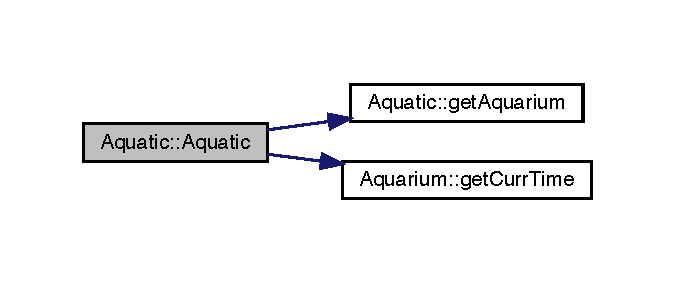
\includegraphics[width=324pt]{class_aquatic_a302075a7330fcdf17dc0fc50ae62ada8_cgraph}
\end{center}
\end{figure}
\mbox{\Hypertarget{class_aquatic_a01426b7729415006ede2c6238fc5849e}\label{class_aquatic_a01426b7729415006ede2c6238fc5849e}} 
\index{Aquatic@{Aquatic}!Aquatic@{Aquatic}}
\index{Aquatic@{Aquatic}!Aquatic@{Aquatic}}
\subsubsection{\texorpdfstring{Aquatic()}{Aquatic()}\hspace{0.1cm}{\footnotesize\ttfamily [2/2]}}
{\footnotesize\ttfamily Aquatic\+::\+Aquatic (\begin{DoxyParamCaption}\item[{double}]{x,  }\item[{double}]{y,  }\item[{double}]{move\+\_\+speed,  }\item[{\mbox{\hyperlink{class_aquarium}{Aquarium}} $\ast$}]{aquarium }\end{DoxyParamCaption})}



A constructor. 

Constructs a new \mbox{\hyperlink{class_aquarium}{Aquarium}} object. 
\begin{DoxyParams}{Parameters}
{\em double} & x Initial x-\/position of the object in the aquarium. \\
\hline
{\em double} & y Initial y-\/position of the object in the aquarium. \\
\hline
{\em double} & move\+\_\+speed Object move speed. \\
\hline
{\em \mbox{\hyperlink{class_aquarium}{Aquarium}}} & $\ast$aquarium The \mbox{\hyperlink{class_aquarium}{Aquarium}} that contains the object. \\
\hline
\end{DoxyParams}
Here is the call graph for this function\+:\nopagebreak
\begin{figure}[H]
\begin{center}
\leavevmode
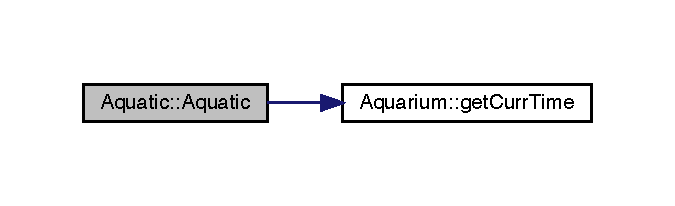
\includegraphics[width=324pt]{class_aquatic_a01426b7729415006ede2c6238fc5849e_cgraph}
\end{center}
\end{figure}


\subsection{Member Function Documentation}
\mbox{\Hypertarget{class_aquatic_a22fdb11e9cfec922fe50638709768276}\label{class_aquatic_a22fdb11e9cfec922fe50638709768276}} 
\index{Aquatic@{Aquatic}!dead@{dead}}
\index{dead@{dead}!Aquatic@{Aquatic}}
\subsubsection{\texorpdfstring{dead()}{dead()}}
{\footnotesize\ttfamily virtual void Aquatic\+::dead (\begin{DoxyParamCaption}{ }\end{DoxyParamCaption})\hspace{0.3cm}{\ttfamily [pure virtual]}}



Executing dead progress. 



Implemented in \mbox{\hyperlink{class_snail_ae80c3d27739aefd6d9c9078c4d17fcc3}{Snail}}, \mbox{\hyperlink{class_guppy_abcdcd74d4c3fdddfc5cc0439c0e512b7}{Guppy}}, \mbox{\hyperlink{class_piranha_a1f30b46fb909558c44eba327e99d5f2e}{Piranha}}, \mbox{\hyperlink{class_coin_af0c650f68a63698691c574fbef940776}{Coin}}, and \mbox{\hyperlink{class_pellet_a50bfc2589da43b06640bc5504e3c689b}{Pellet}}.

\mbox{\Hypertarget{class_aquatic_aa84812ff8347a11345b9c8231c1375cc}\label{class_aquatic_aa84812ff8347a11345b9c8231c1375cc}} 
\index{Aquatic@{Aquatic}!get\+Aquarium@{get\+Aquarium}}
\index{get\+Aquarium@{get\+Aquarium}!Aquatic@{Aquatic}}
\subsubsection{\texorpdfstring{get\+Aquarium()}{getAquarium()}}
{\footnotesize\ttfamily \mbox{\hyperlink{class_aquarium}{Aquarium}} $\ast$ Aquatic\+::get\+Aquarium (\begin{DoxyParamCaption}{ }\end{DoxyParamCaption})}



Getter for aquarium. 

\begin{DoxyReturn}{Returns}
\mbox{\hyperlink{class_aquarium}{Aquarium}} $\ast$aquarium Pointer to the \mbox{\hyperlink{class_aquarium}{Aquarium}} that contains the object. 
\end{DoxyReturn}
Here is the caller graph for this function\+:
\nopagebreak
\begin{figure}[H]
\begin{center}
\leavevmode
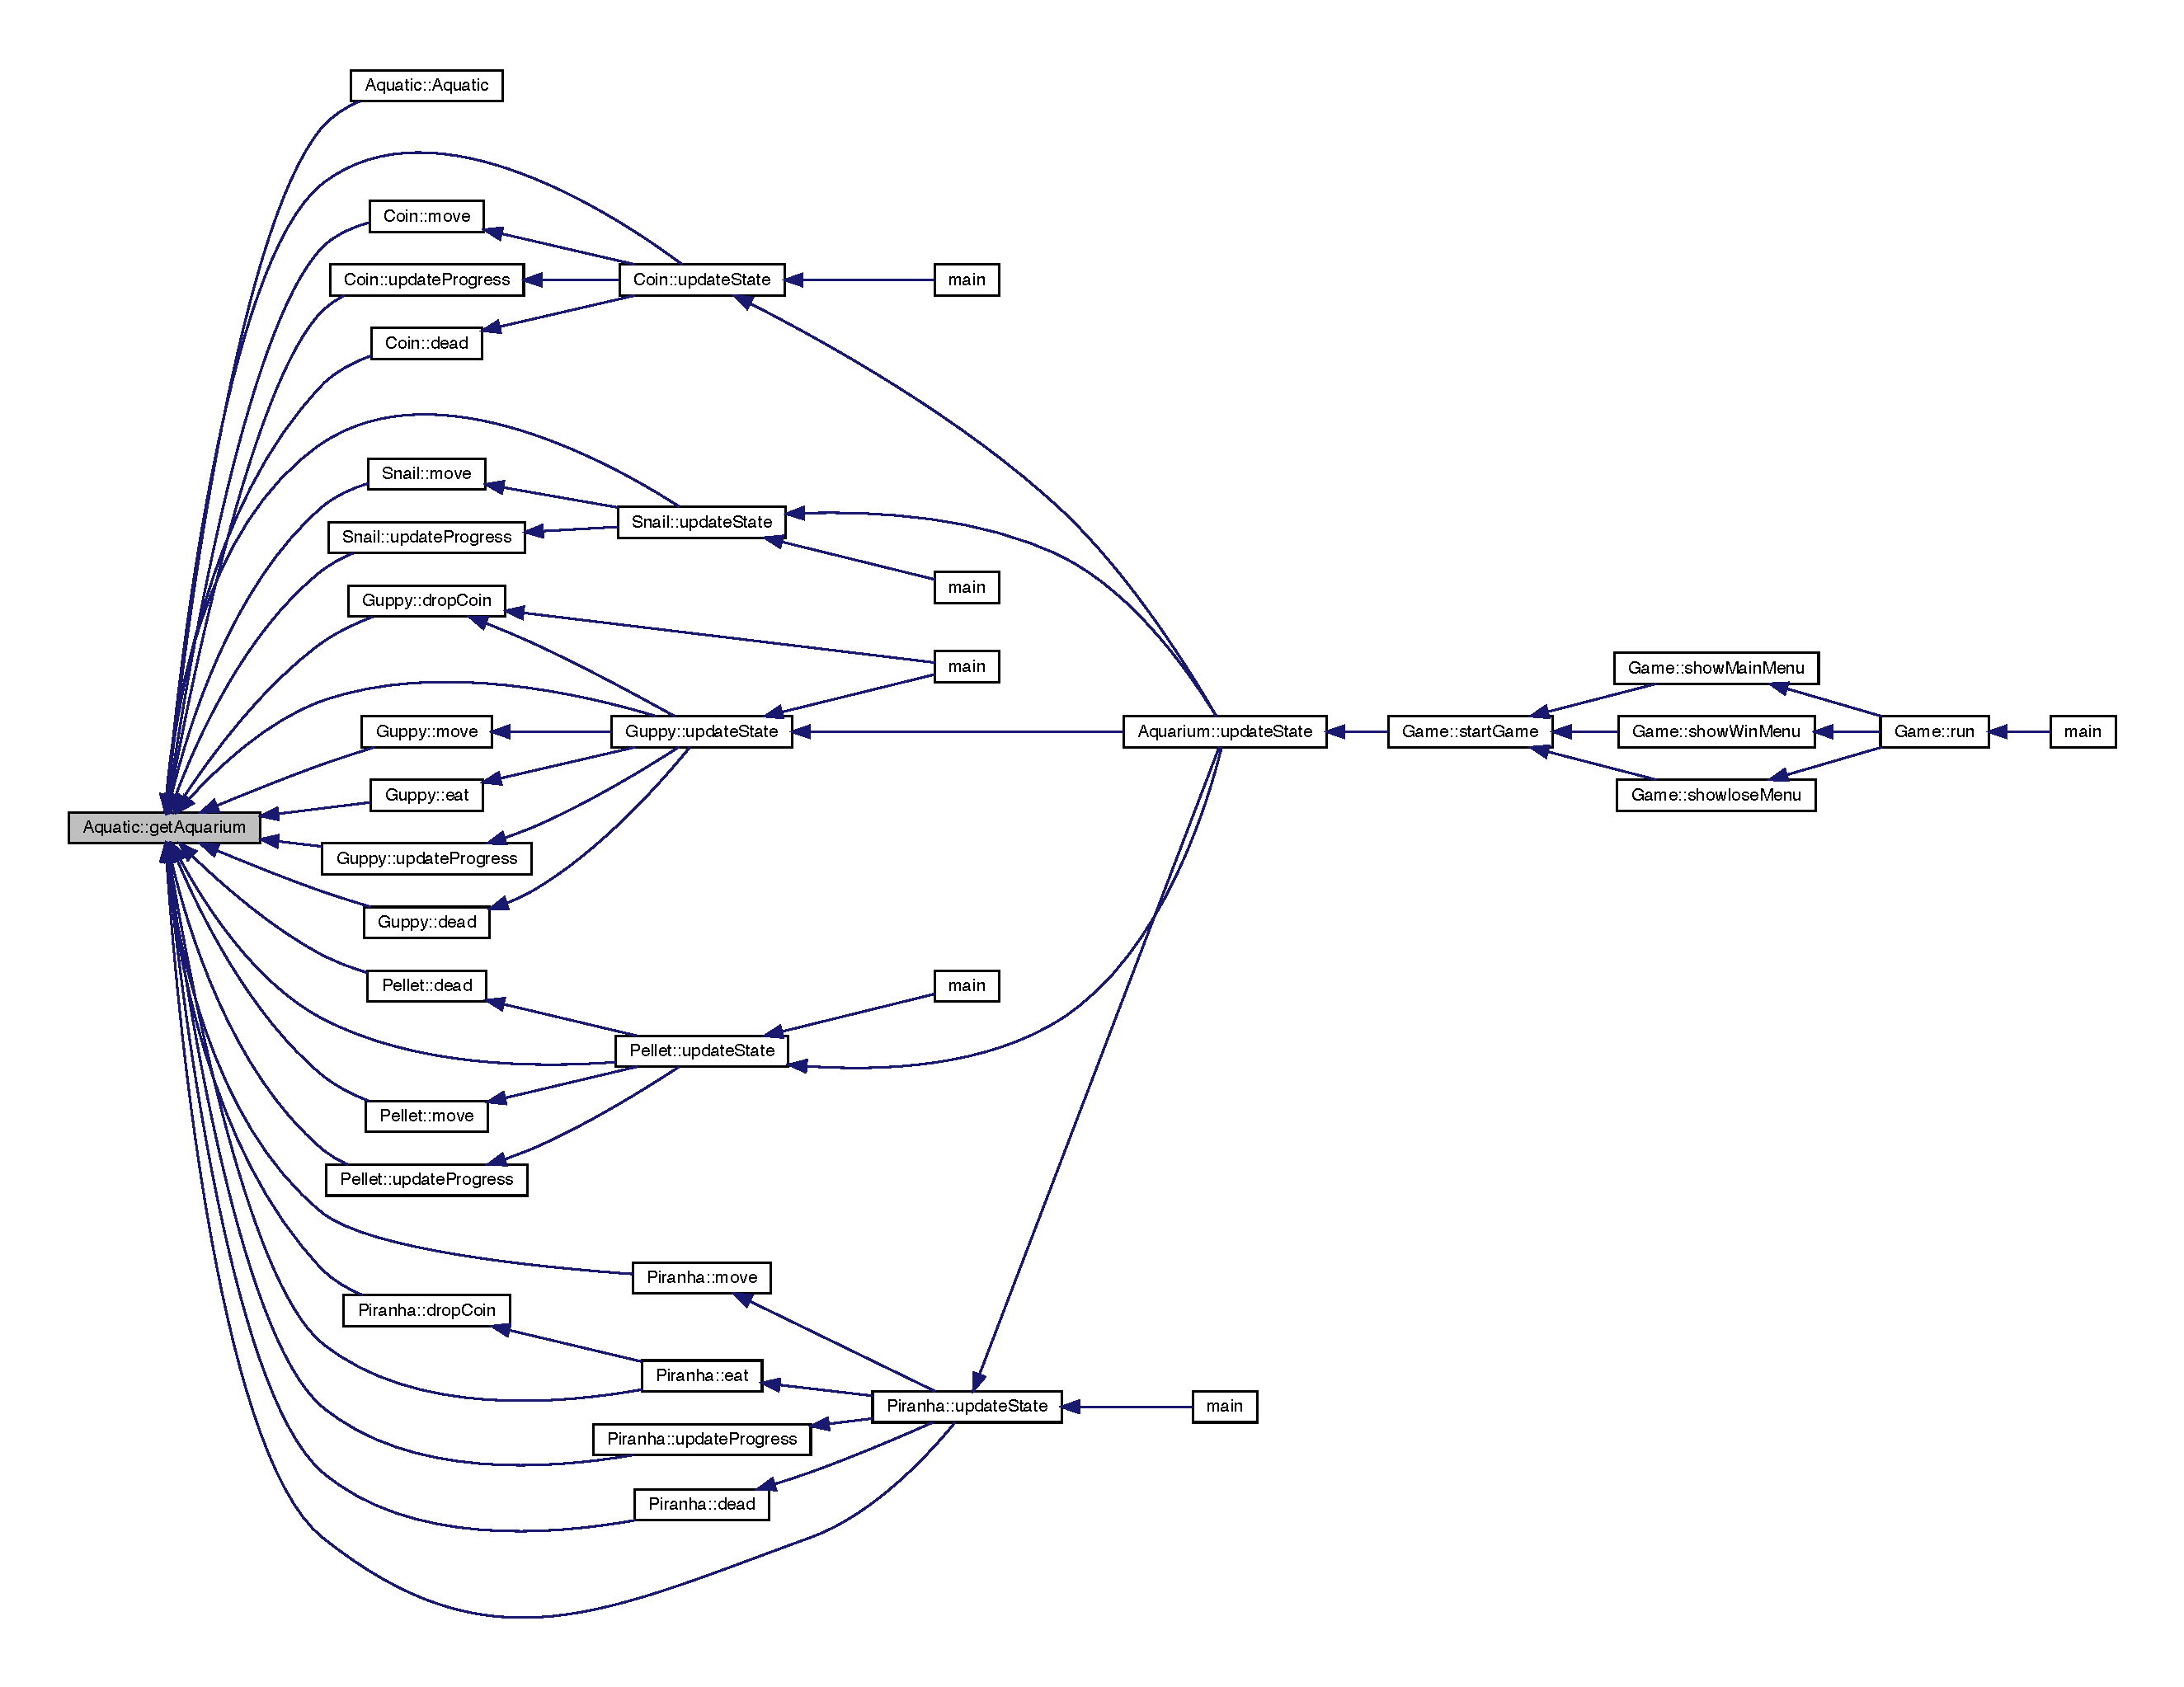
\includegraphics[width=350pt]{class_aquatic_aa84812ff8347a11345b9c8231c1375cc_icgraph}
\end{center}
\end{figure}
\mbox{\Hypertarget{class_aquatic_aba770b1c9ca9481712a6963e7e8e2919}\label{class_aquatic_aba770b1c9ca9481712a6963e7e8e2919}} 
\index{Aquatic@{Aquatic}!get\+Last\+Curr\+Time@{get\+Last\+Curr\+Time}}
\index{get\+Last\+Curr\+Time@{get\+Last\+Curr\+Time}!Aquatic@{Aquatic}}
\subsubsection{\texorpdfstring{get\+Last\+Curr\+Time()}{getLastCurrTime()}}
{\footnotesize\ttfamily double Aquatic\+::get\+Last\+Curr\+Time (\begin{DoxyParamCaption}{ }\end{DoxyParamCaption}) const}



Getter for last\+\_\+curr\+\_\+time. 

\begin{DoxyReturn}{Returns}
double last\+\_\+curr\+\_\+time The last time the object was updated. 
\end{DoxyReturn}
Here is the caller graph for this function\+:
\nopagebreak
\begin{figure}[H]
\begin{center}
\leavevmode
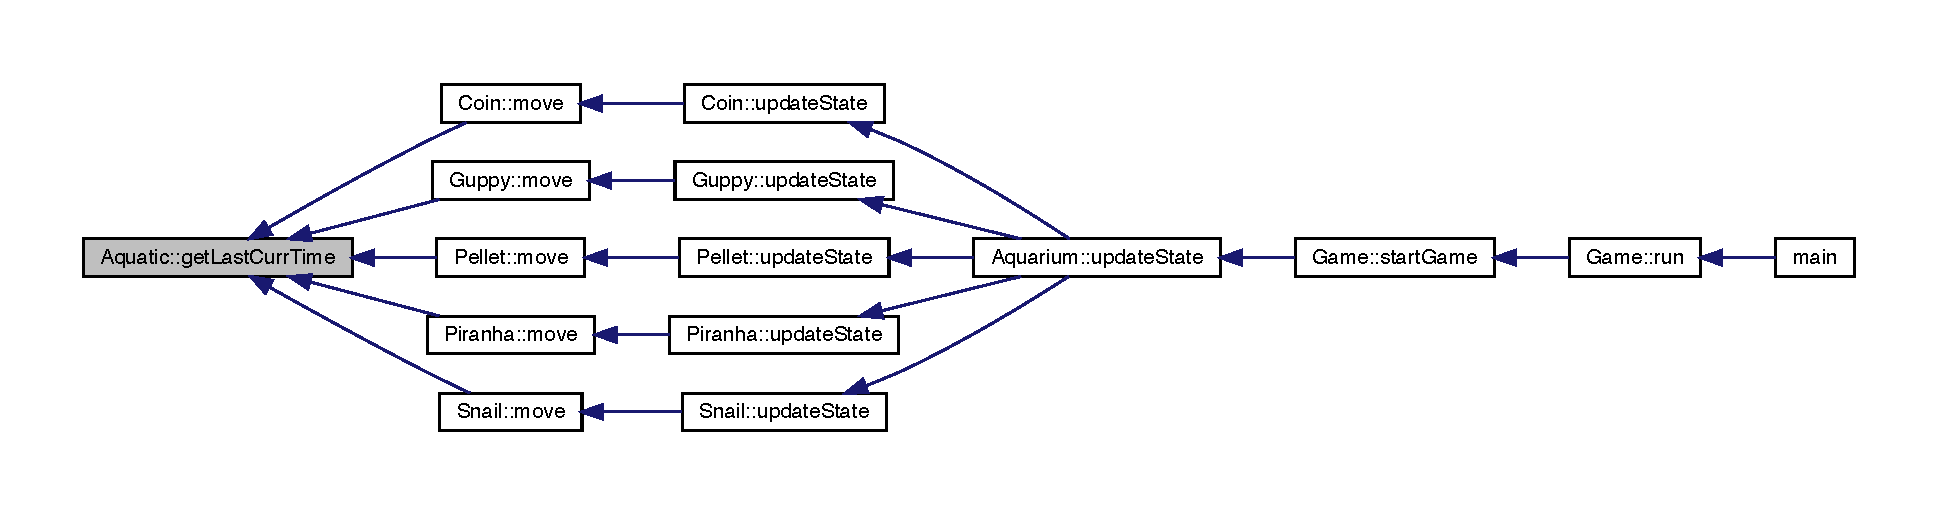
\includegraphics[width=350pt]{class_aquatic_aba770b1c9ca9481712a6963e7e8e2919_icgraph}
\end{center}
\end{figure}
\mbox{\Hypertarget{class_aquatic_a60e1c0f173d0b37adce3cdd3d92efea0}\label{class_aquatic_a60e1c0f173d0b37adce3cdd3d92efea0}} 
\index{Aquatic@{Aquatic}!get\+Last\+Progress\+Time@{get\+Last\+Progress\+Time}}
\index{get\+Last\+Progress\+Time@{get\+Last\+Progress\+Time}!Aquatic@{Aquatic}}
\subsubsection{\texorpdfstring{get\+Last\+Progress\+Time()}{getLastProgressTime()}}
{\footnotesize\ttfamily double Aquatic\+::get\+Last\+Progress\+Time (\begin{DoxyParamCaption}{ }\end{DoxyParamCaption})}



Getter for last\+\_\+progress\+\_\+times. 

\begin{DoxyReturn}{Returns}
double last\+\_\+progress\+\_\+time The last time the object progress time was updated. 
\end{DoxyReturn}
Here is the caller graph for this function\+:
\nopagebreak
\begin{figure}[H]
\begin{center}
\leavevmode
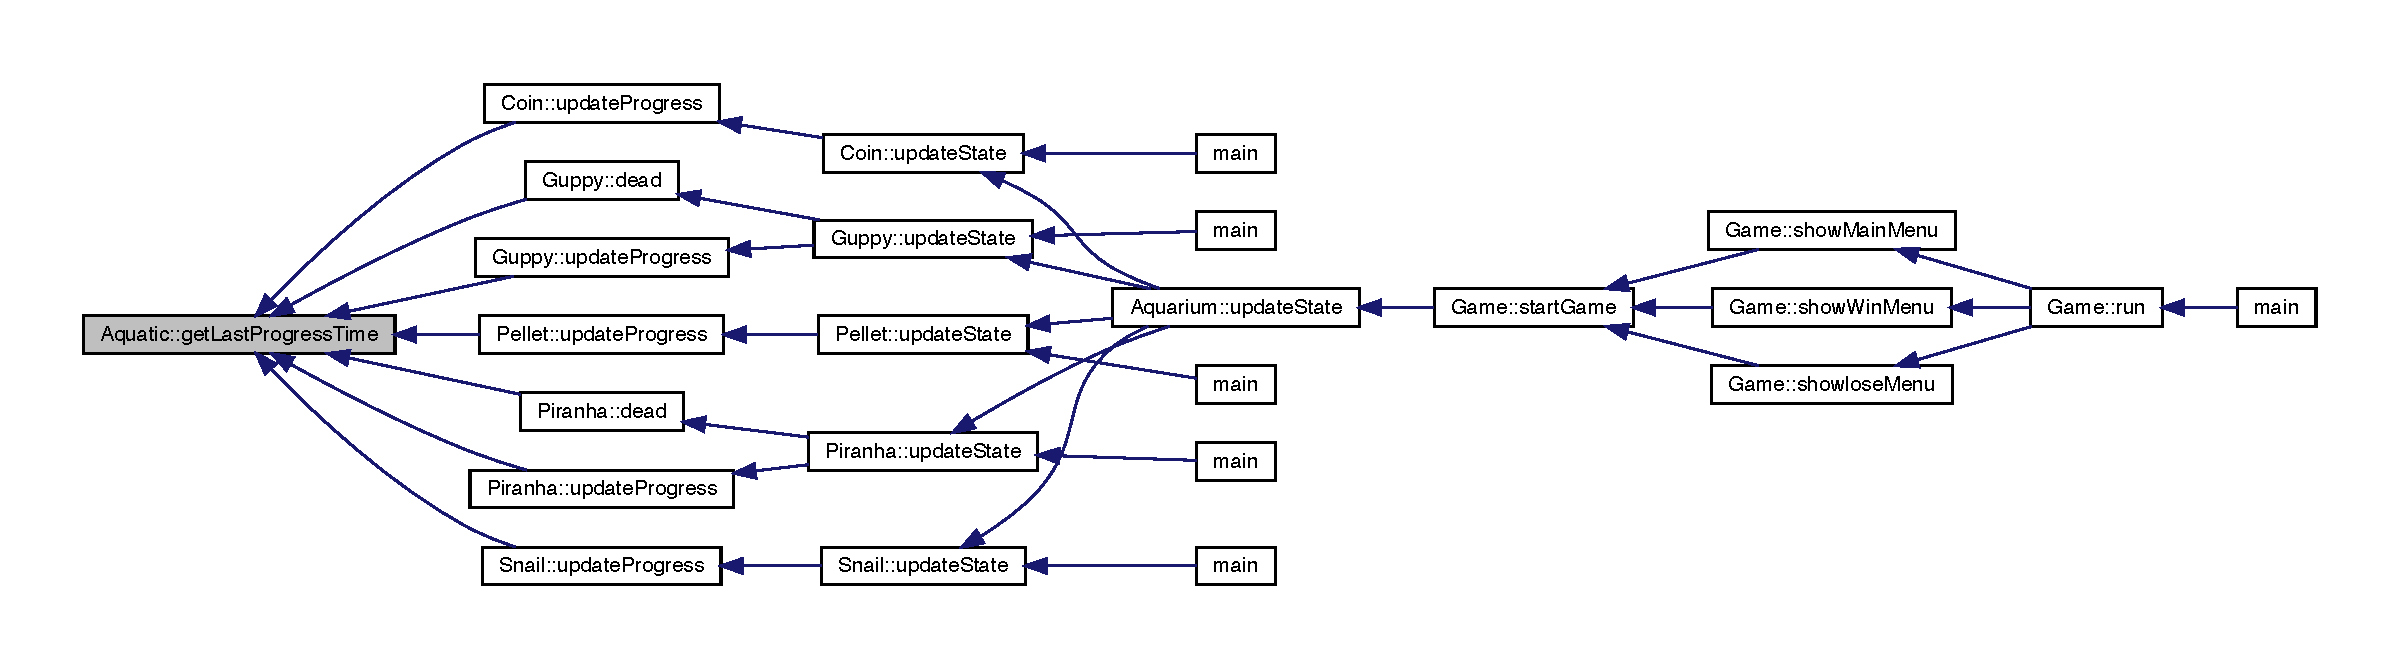
\includegraphics[width=350pt]{class_aquatic_a60e1c0f173d0b37adce3cdd3d92efea0_icgraph}
\end{center}
\end{figure}
\mbox{\Hypertarget{class_aquatic_a4153178bfefdc57cbcd05fe44054dac9}\label{class_aquatic_a4153178bfefdc57cbcd05fe44054dac9}} 
\index{Aquatic@{Aquatic}!get\+Move\+Speed@{get\+Move\+Speed}}
\index{get\+Move\+Speed@{get\+Move\+Speed}!Aquatic@{Aquatic}}
\subsubsection{\texorpdfstring{get\+Move\+Speed()}{getMoveSpeed()}}
{\footnotesize\ttfamily double Aquatic\+::get\+Move\+Speed (\begin{DoxyParamCaption}{ }\end{DoxyParamCaption}) const}



Getter for move\+\_\+speed. 

\begin{DoxyReturn}{Returns}
double move\+\_\+speed 
\end{DoxyReturn}
Here is the caller graph for this function\+:
\nopagebreak
\begin{figure}[H]
\begin{center}
\leavevmode
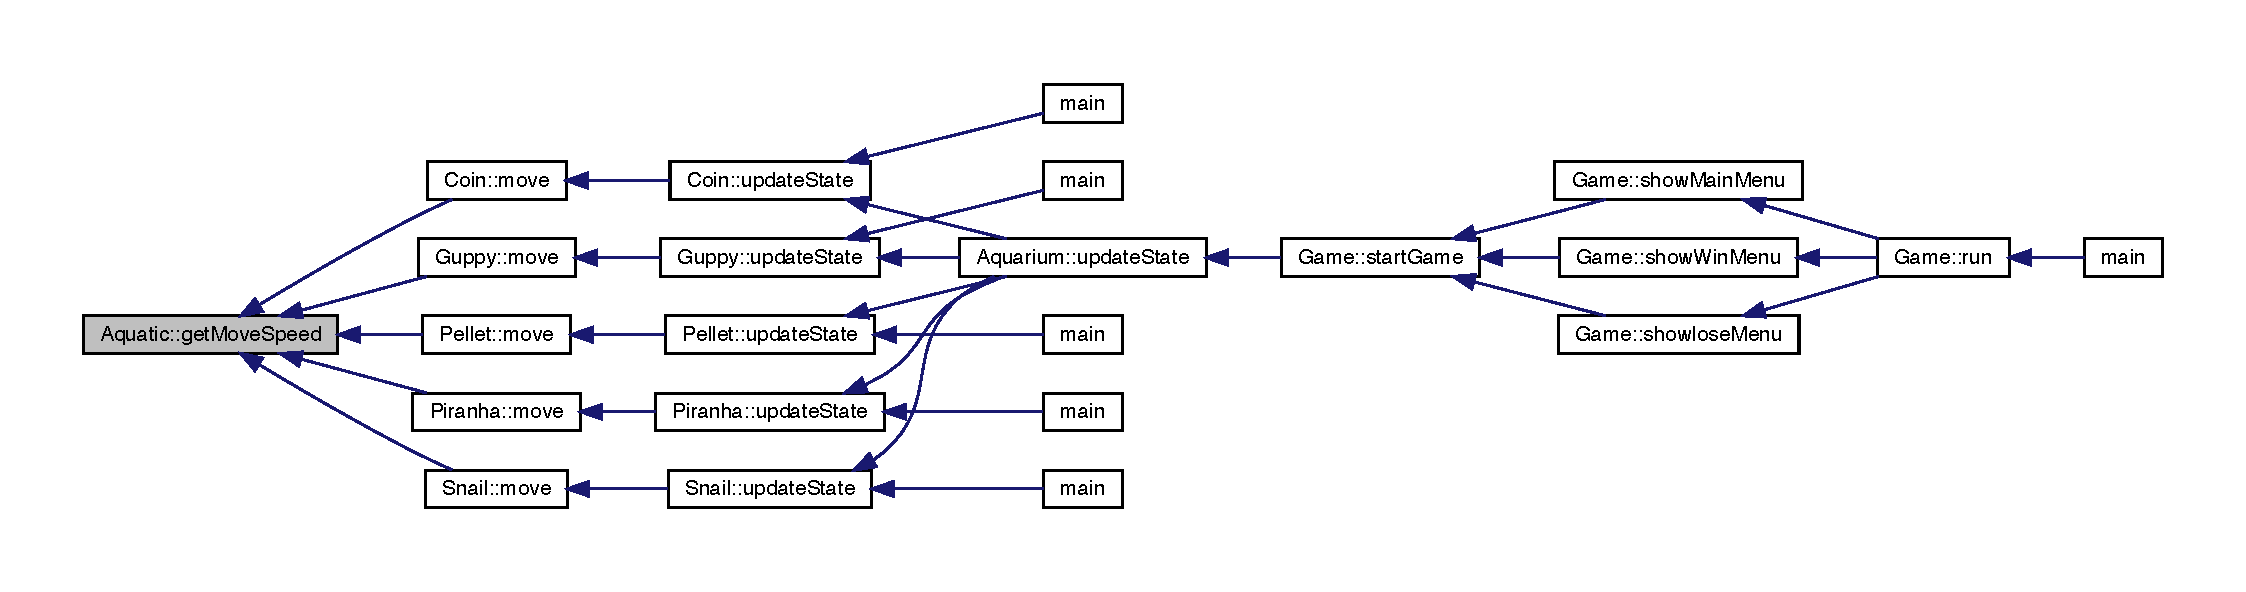
\includegraphics[width=350pt]{class_aquatic_a4153178bfefdc57cbcd05fe44054dac9_icgraph}
\end{center}
\end{figure}
\mbox{\Hypertarget{class_aquatic_a0de76e489d82ccad52dec32a1978850c}\label{class_aquatic_a0de76e489d82ccad52dec32a1978850c}} 
\index{Aquatic@{Aquatic}!get\+Progress@{get\+Progress}}
\index{get\+Progress@{get\+Progress}!Aquatic@{Aquatic}}
\subsubsection{\texorpdfstring{get\+Progress()}{getProgress()}}
{\footnotesize\ttfamily int Aquatic\+::get\+Progress (\begin{DoxyParamCaption}{ }\end{DoxyParamCaption})}



Getter for progress. 

\begin{DoxyReturn}{Returns}
int progress The progress of the state. 
\end{DoxyReturn}
Here is the caller graph for this function\+:
\nopagebreak
\begin{figure}[H]
\begin{center}
\leavevmode
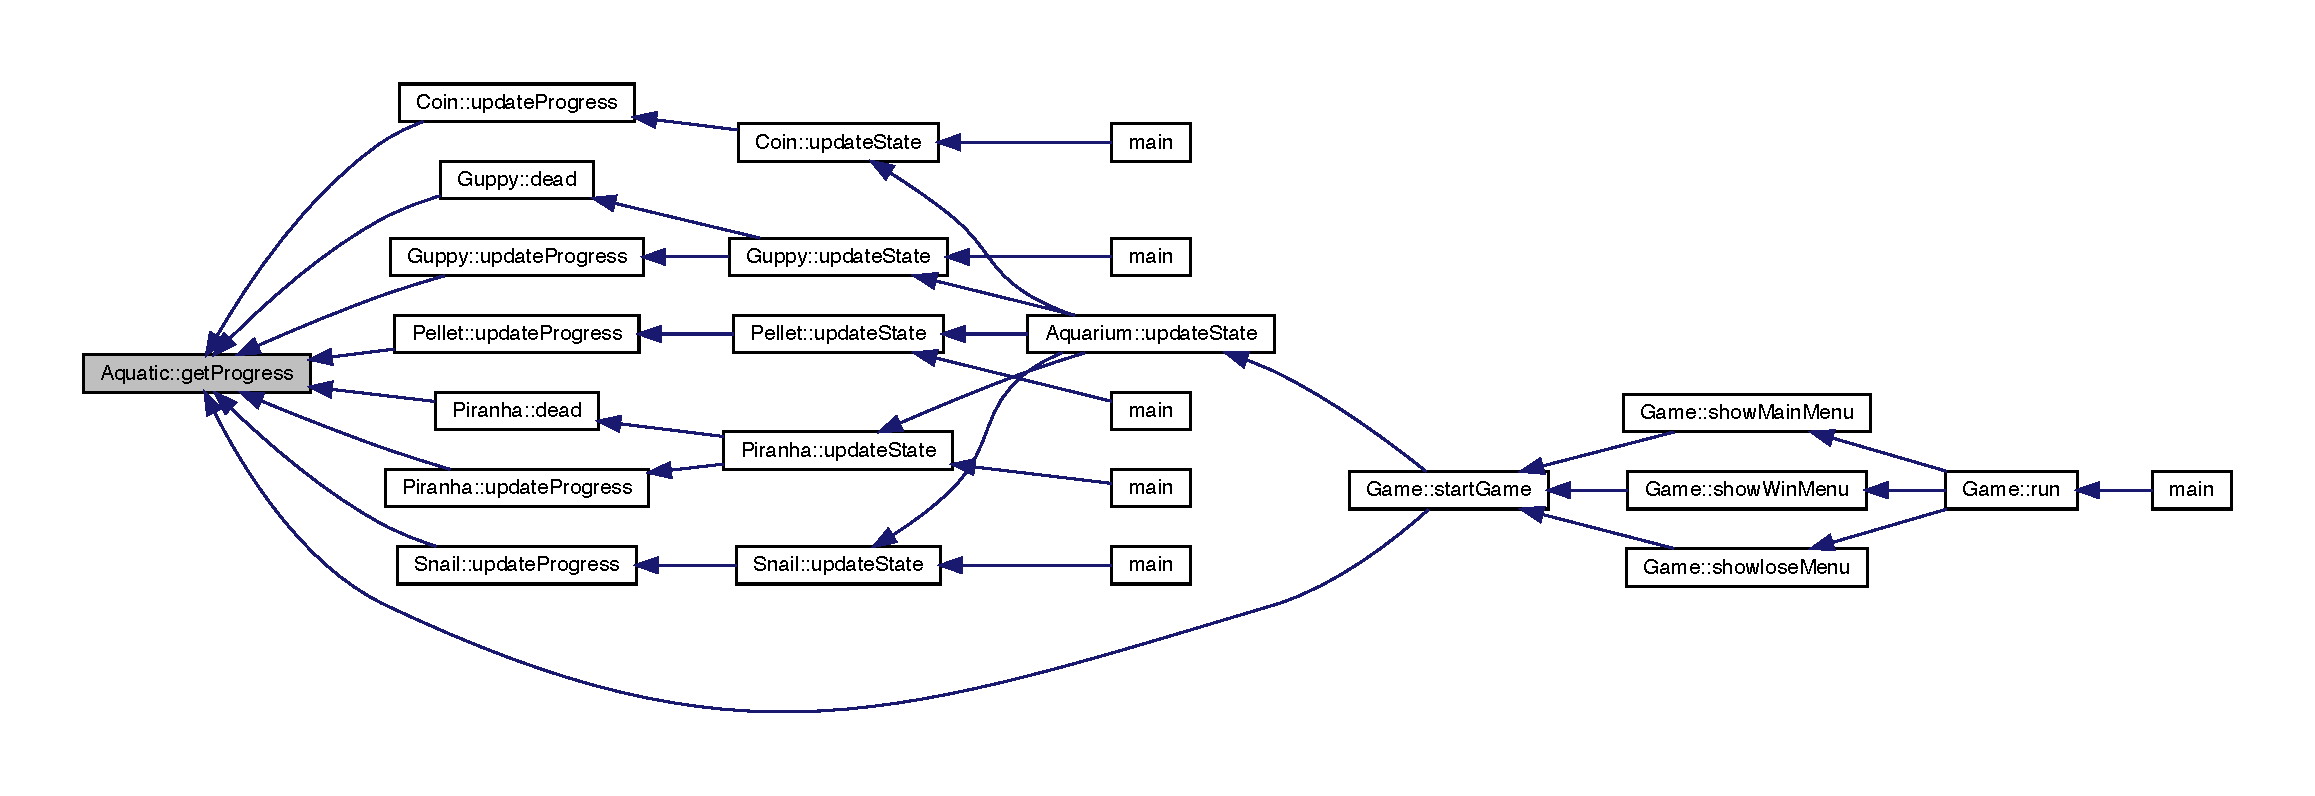
\includegraphics[width=350pt]{class_aquatic_a0de76e489d82ccad52dec32a1978850c_icgraph}
\end{center}
\end{figure}
\mbox{\Hypertarget{class_aquatic_a3d73a0494585841ebd2acaee7281ece5}\label{class_aquatic_a3d73a0494585841ebd2acaee7281ece5}} 
\index{Aquatic@{Aquatic}!get\+State@{get\+State}}
\index{get\+State@{get\+State}!Aquatic@{Aquatic}}
\subsubsection{\texorpdfstring{get\+State()}{getState()}}
{\footnotesize\ttfamily \mbox{\hyperlink{_constants_8hpp_a5d74787dedbc4e11c1ab15bf487e61f8}{State}} Aquatic\+::get\+State (\begin{DoxyParamCaption}{ }\end{DoxyParamCaption})}



Getter for state. 

\begin{DoxyReturn}{Returns}
State state The current state of the \mbox{\hyperlink{class_aquatic}{Aquatic}} \+: moving\+Right, moving\+Left, turning\+Right, turning\+Left, still\+Left, still\+Right, dead\+Left, dead\+Right 
\end{DoxyReturn}
Here is the caller graph for this function\+:
\nopagebreak
\begin{figure}[H]
\begin{center}
\leavevmode
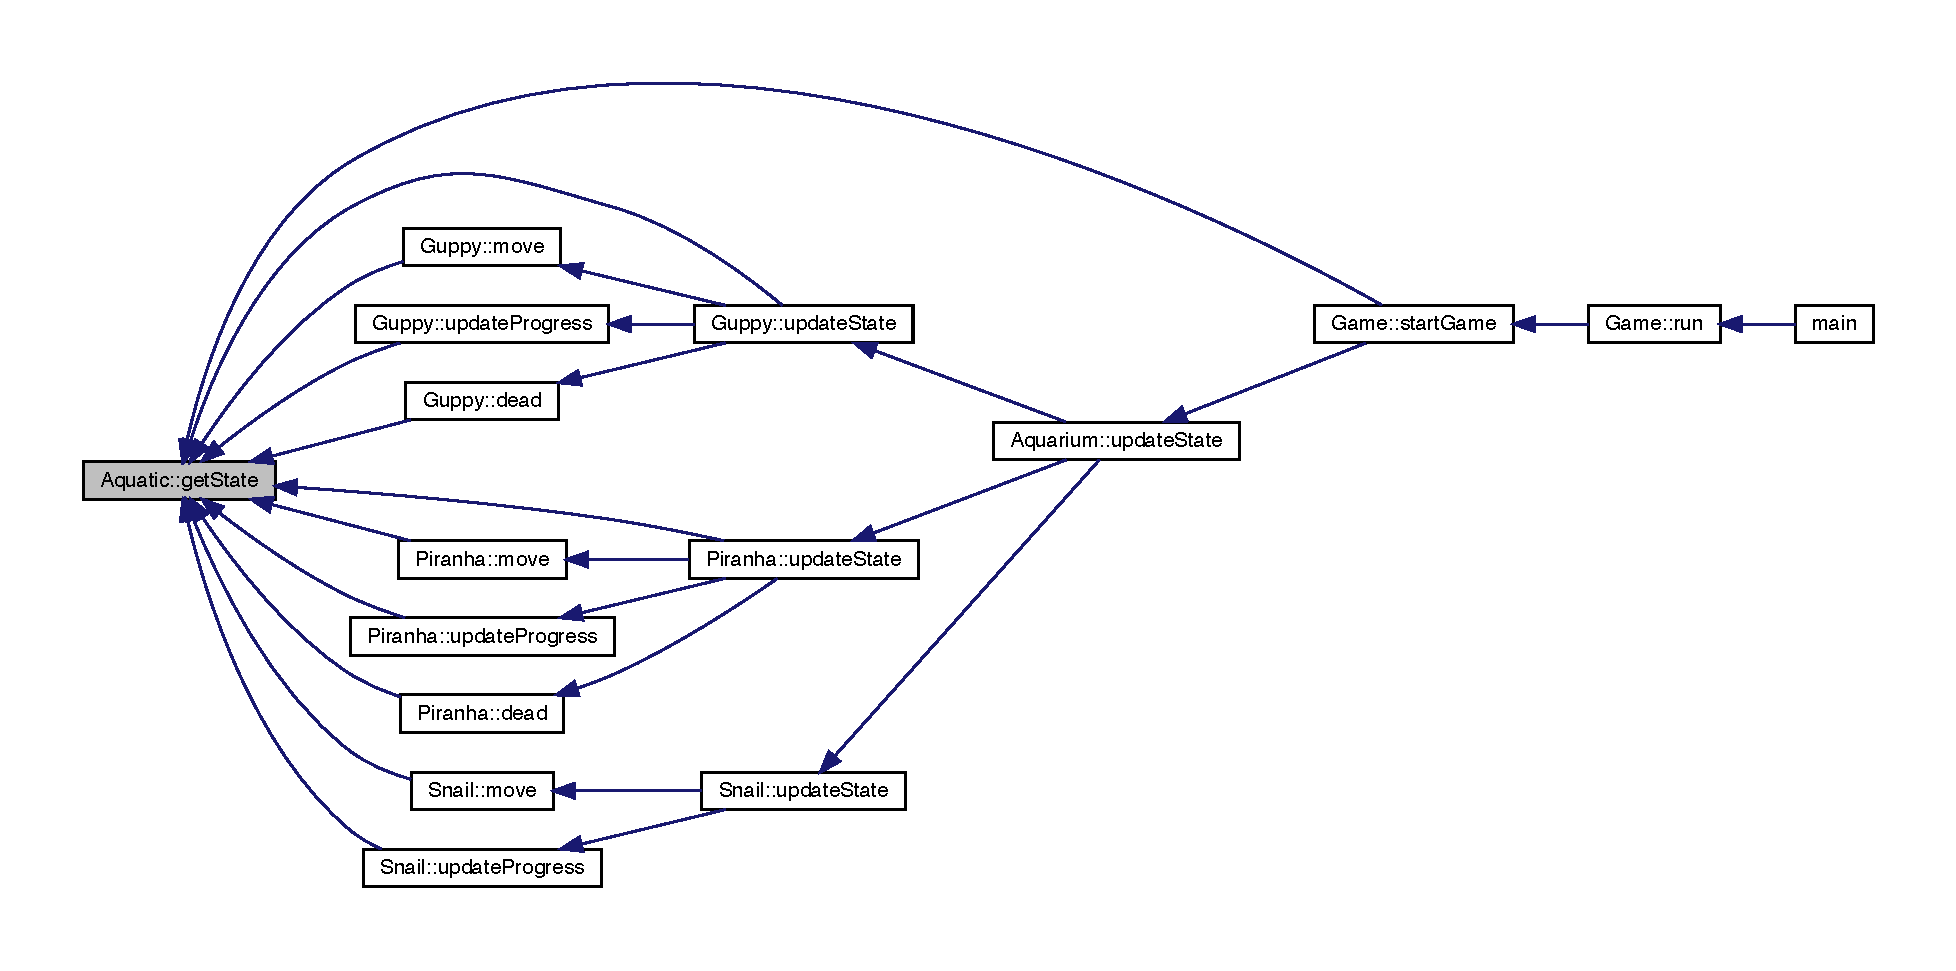
\includegraphics[width=350pt]{class_aquatic_a3d73a0494585841ebd2acaee7281ece5_icgraph}
\end{center}
\end{figure}
\mbox{\Hypertarget{class_aquatic_ab59ba97a4876a0e3ae8b85c1915a82f9}\label{class_aquatic_ab59ba97a4876a0e3ae8b85c1915a82f9}} 
\index{Aquatic@{Aquatic}!getX@{getX}}
\index{getX@{getX}!Aquatic@{Aquatic}}
\subsubsection{\texorpdfstring{get\+X()}{getX()}}
{\footnotesize\ttfamily double Aquatic\+::getX (\begin{DoxyParamCaption}{ }\end{DoxyParamCaption})}



Getter for x. 

\begin{DoxyReturn}{Returns}
double x x-\/axis position of the object. 
\end{DoxyReturn}
Here is the caller graph for this function\+:
\nopagebreak
\begin{figure}[H]
\begin{center}
\leavevmode
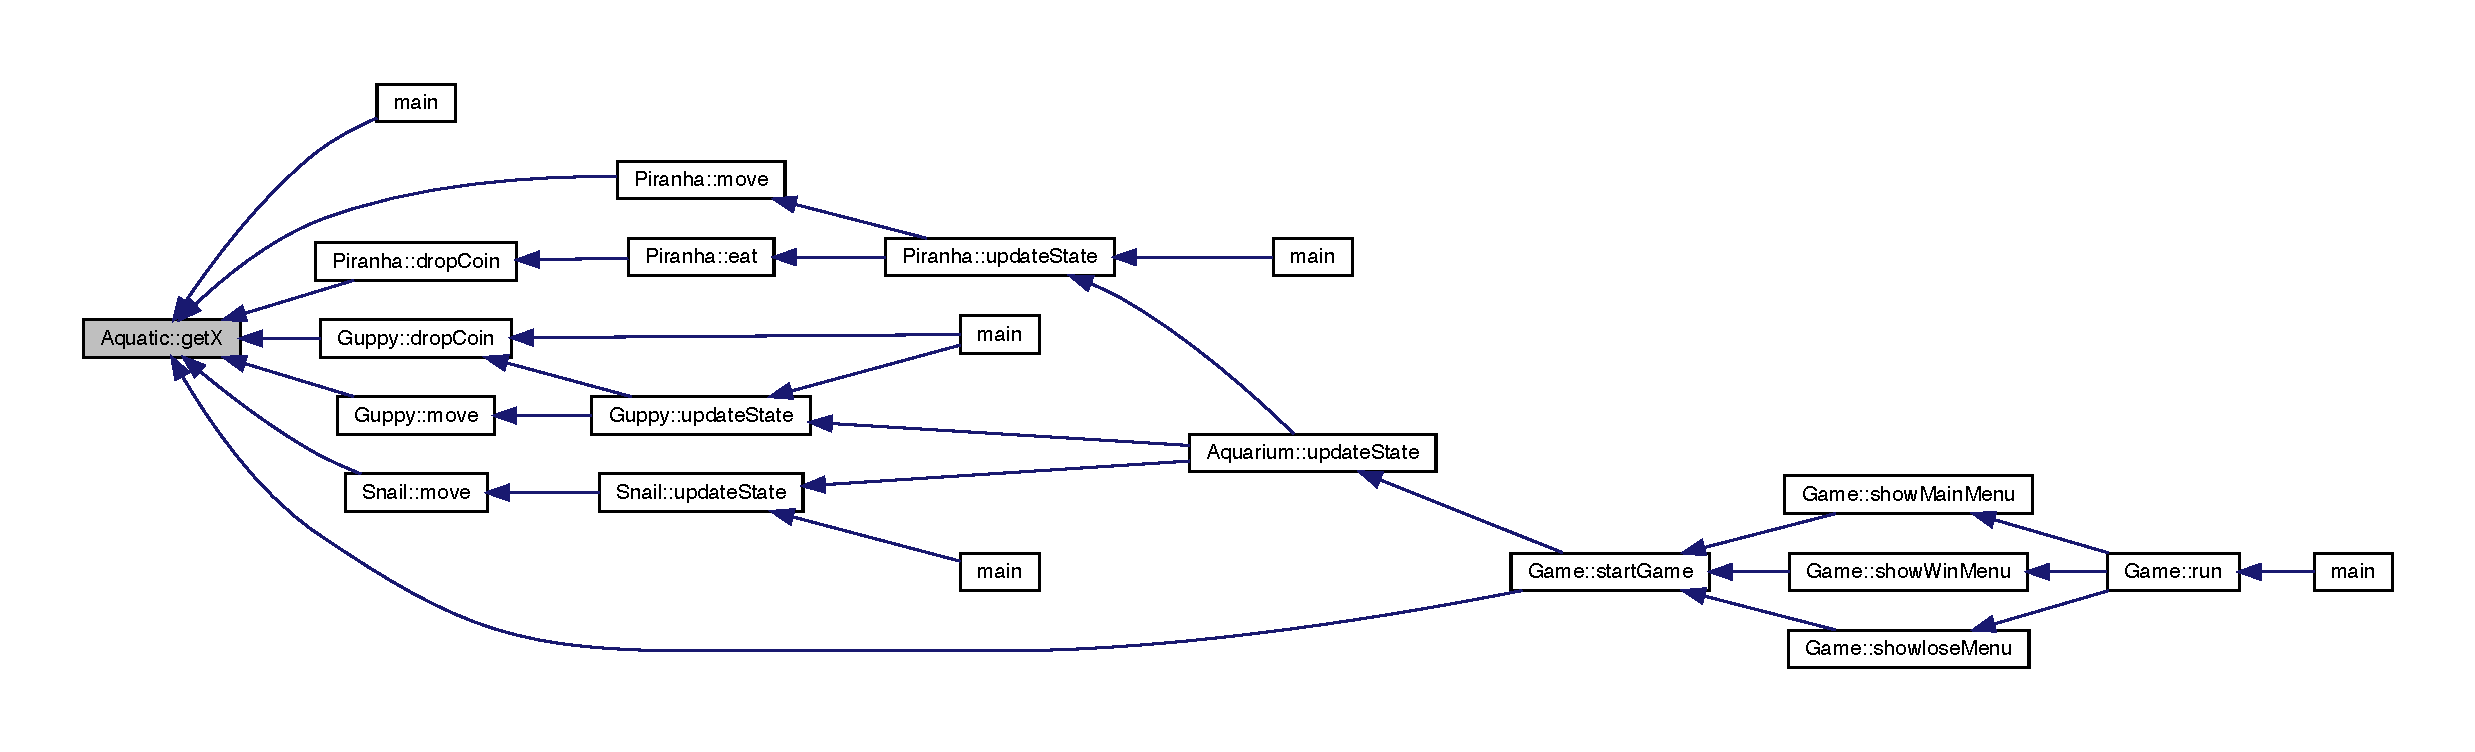
\includegraphics[width=350pt]{class_aquatic_ab59ba97a4876a0e3ae8b85c1915a82f9_icgraph}
\end{center}
\end{figure}
\mbox{\Hypertarget{class_aquatic_aadfede87649072d59192d923200b6fc3}\label{class_aquatic_aadfede87649072d59192d923200b6fc3}} 
\index{Aquatic@{Aquatic}!getY@{getY}}
\index{getY@{getY}!Aquatic@{Aquatic}}
\subsubsection{\texorpdfstring{get\+Y()}{getY()}}
{\footnotesize\ttfamily double Aquatic\+::getY (\begin{DoxyParamCaption}{ }\end{DoxyParamCaption})}



Getter for y. 

\begin{DoxyReturn}{Returns}
double y y-\/axis position of the object. 
\end{DoxyReturn}
Here is the caller graph for this function\+:
\nopagebreak
\begin{figure}[H]
\begin{center}
\leavevmode
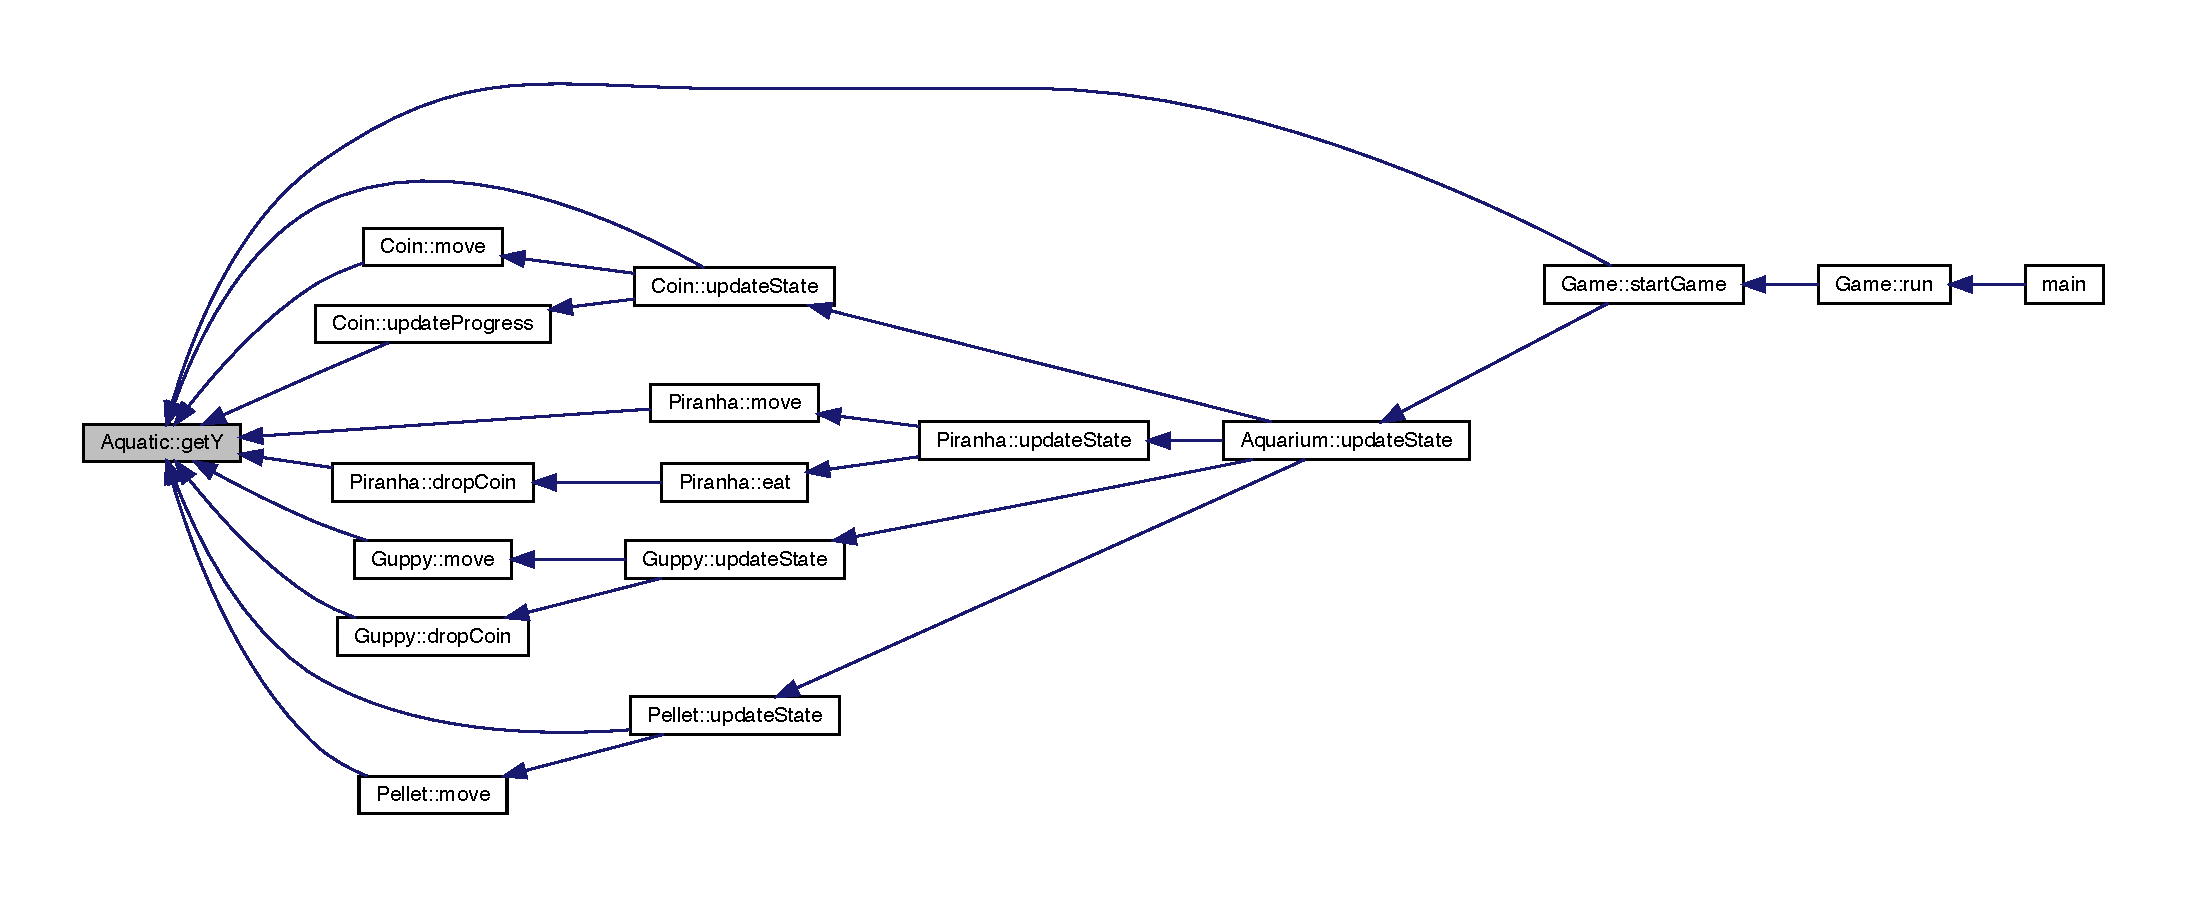
\includegraphics[width=350pt]{class_aquatic_aadfede87649072d59192d923200b6fc3_icgraph}
\end{center}
\end{figure}
\mbox{\Hypertarget{class_aquatic_a2c438132d8b625d3c2187ff5735193a0}\label{class_aquatic_a2c438132d8b625d3c2187ff5735193a0}} 
\index{Aquatic@{Aquatic}!is\+Inside@{is\+Inside}}
\index{is\+Inside@{is\+Inside}!Aquatic@{Aquatic}}
\subsubsection{\texorpdfstring{is\+Inside()}{isInside()}}
{\footnotesize\ttfamily bool Aquatic\+::is\+Inside (\begin{DoxyParamCaption}{ }\end{DoxyParamCaption})}



Check whether the object is inside the aquarium or not. 

\begin{DoxyReturn}{Returns}
bool true if inside 
\end{DoxyReturn}
Here is the call graph for this function\+:\nopagebreak
\begin{figure}[H]
\begin{center}
\leavevmode
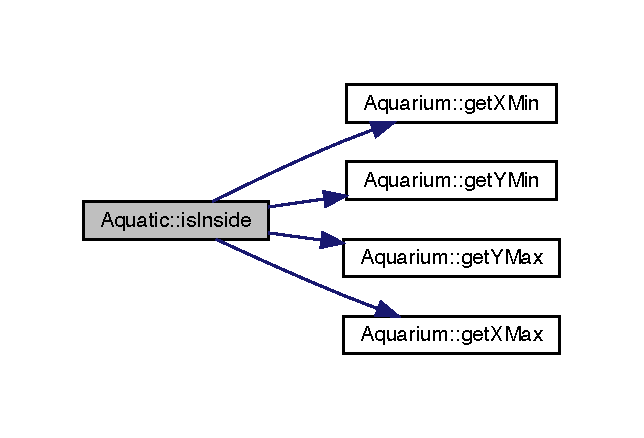
\includegraphics[width=309pt]{class_aquatic_a2c438132d8b625d3c2187ff5735193a0_cgraph}
\end{center}
\end{figure}
Here is the caller graph for this function\+:
\nopagebreak
\begin{figure}[H]
\begin{center}
\leavevmode
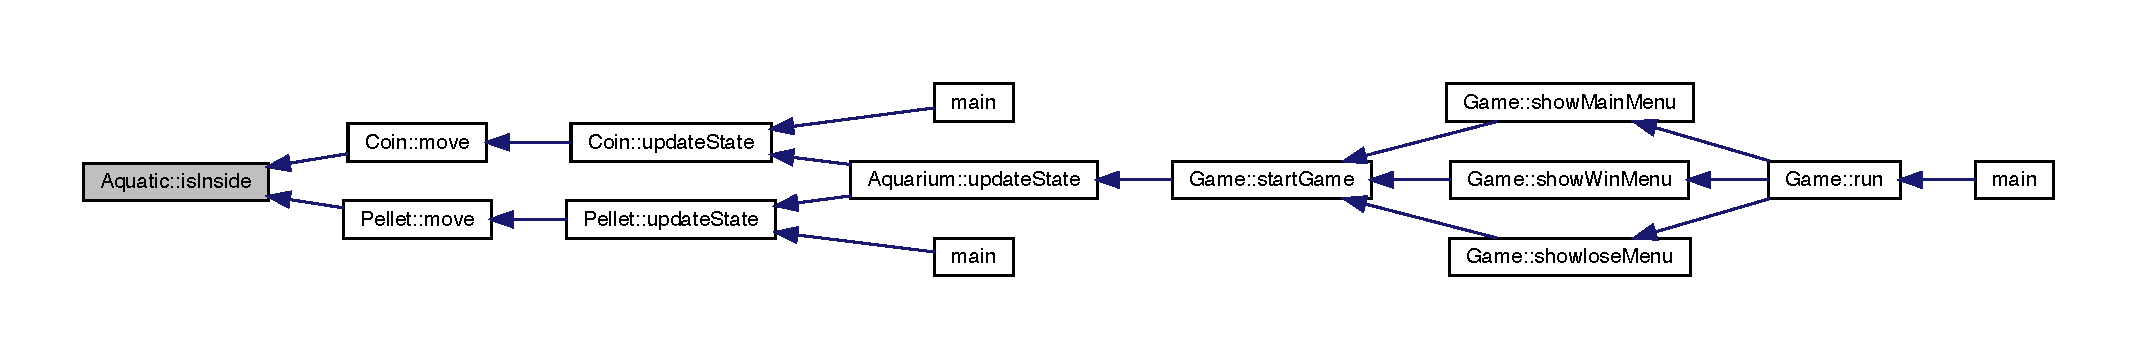
\includegraphics[width=350pt]{class_aquatic_a2c438132d8b625d3c2187ff5735193a0_icgraph}
\end{center}
\end{figure}
\mbox{\Hypertarget{class_aquatic_a962e93c804814eeaf3cea6e26698eef7}\label{class_aquatic_a962e93c804814eeaf3cea6e26698eef7}} 
\index{Aquatic@{Aquatic}!move@{move}}
\index{move@{move}!Aquatic@{Aquatic}}
\subsubsection{\texorpdfstring{move()}{move()}}
{\footnotesize\ttfamily virtual void Aquatic\+::move (\begin{DoxyParamCaption}{ }\end{DoxyParamCaption})\hspace{0.3cm}{\ttfamily [pure virtual]}}



Moves the object independently. 



Implemented in \mbox{\hyperlink{class_snail_af5892ec122d9199480c813b74488256b}{Snail}}, \mbox{\hyperlink{class_guppy_ae6002948d74b3741bed34a7311be4377}{Guppy}}, \mbox{\hyperlink{class_piranha_a6b86e73b3e5a57ee0fdb768c24ab9b67}{Piranha}}, \mbox{\hyperlink{class_coin_ab62bca5834489b9b483deaa3ca3470e9}{Coin}}, and \mbox{\hyperlink{class_pellet_a7385101b04083be663ae465c38fd2a4d}{Pellet}}.

\mbox{\Hypertarget{class_aquatic_ae2fa11b1ff4a3763a7a7bd4924f6c1eb}\label{class_aquatic_ae2fa11b1ff4a3763a7a7bd4924f6c1eb}} 
\index{Aquatic@{Aquatic}!set\+Last\+Curr\+Time@{set\+Last\+Curr\+Time}}
\index{set\+Last\+Curr\+Time@{set\+Last\+Curr\+Time}!Aquatic@{Aquatic}}
\subsubsection{\texorpdfstring{set\+Last\+Curr\+Time()}{setLastCurrTime()}}
{\footnotesize\ttfamily void Aquatic\+::set\+Last\+Curr\+Time (\begin{DoxyParamCaption}\item[{double}]{t }\end{DoxyParamCaption})}



Setter for curr\+\_\+time. 


\begin{DoxyParams}{Parameters}
{\em double} & current time \\
\hline
\end{DoxyParams}
Here is the caller graph for this function\+:
\nopagebreak
\begin{figure}[H]
\begin{center}
\leavevmode
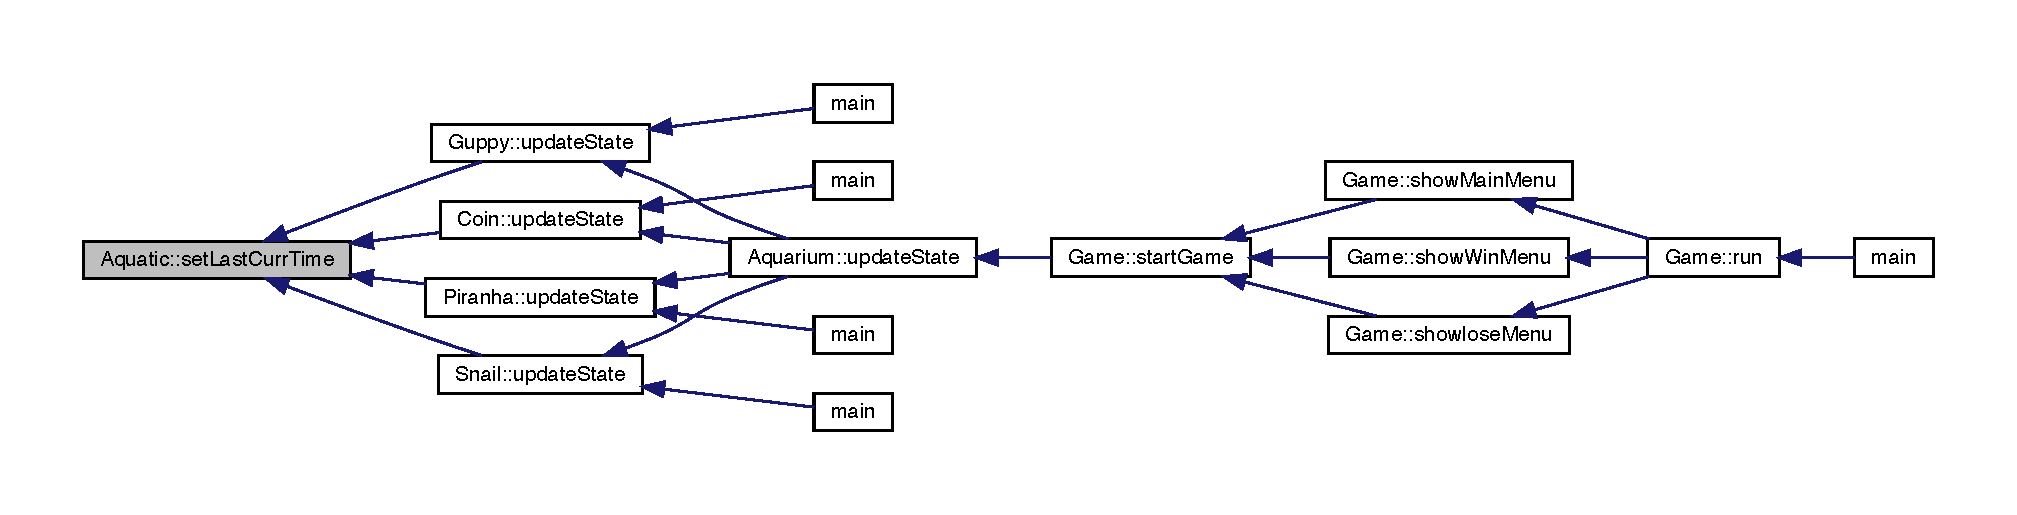
\includegraphics[width=350pt]{class_aquatic_ae2fa11b1ff4a3763a7a7bd4924f6c1eb_icgraph}
\end{center}
\end{figure}
\mbox{\Hypertarget{class_aquatic_a50e51e4b7bfd7f46d3c43bde27e0a5d8}\label{class_aquatic_a50e51e4b7bfd7f46d3c43bde27e0a5d8}} 
\index{Aquatic@{Aquatic}!set\+Last\+Progress\+Time@{set\+Last\+Progress\+Time}}
\index{set\+Last\+Progress\+Time@{set\+Last\+Progress\+Time}!Aquatic@{Aquatic}}
\subsubsection{\texorpdfstring{set\+Last\+Progress\+Time()}{setLastProgressTime()}}
{\footnotesize\ttfamily void Aquatic\+::set\+Last\+Progress\+Time (\begin{DoxyParamCaption}\item[{double}]{t }\end{DoxyParamCaption})}



Setter for last\+\_\+progress\+\_\+time. 


\begin{DoxyParams}{Parameters}
{\em double} & last progress time \\
\hline
\end{DoxyParams}
Here is the caller graph for this function\+:
\nopagebreak
\begin{figure}[H]
\begin{center}
\leavevmode
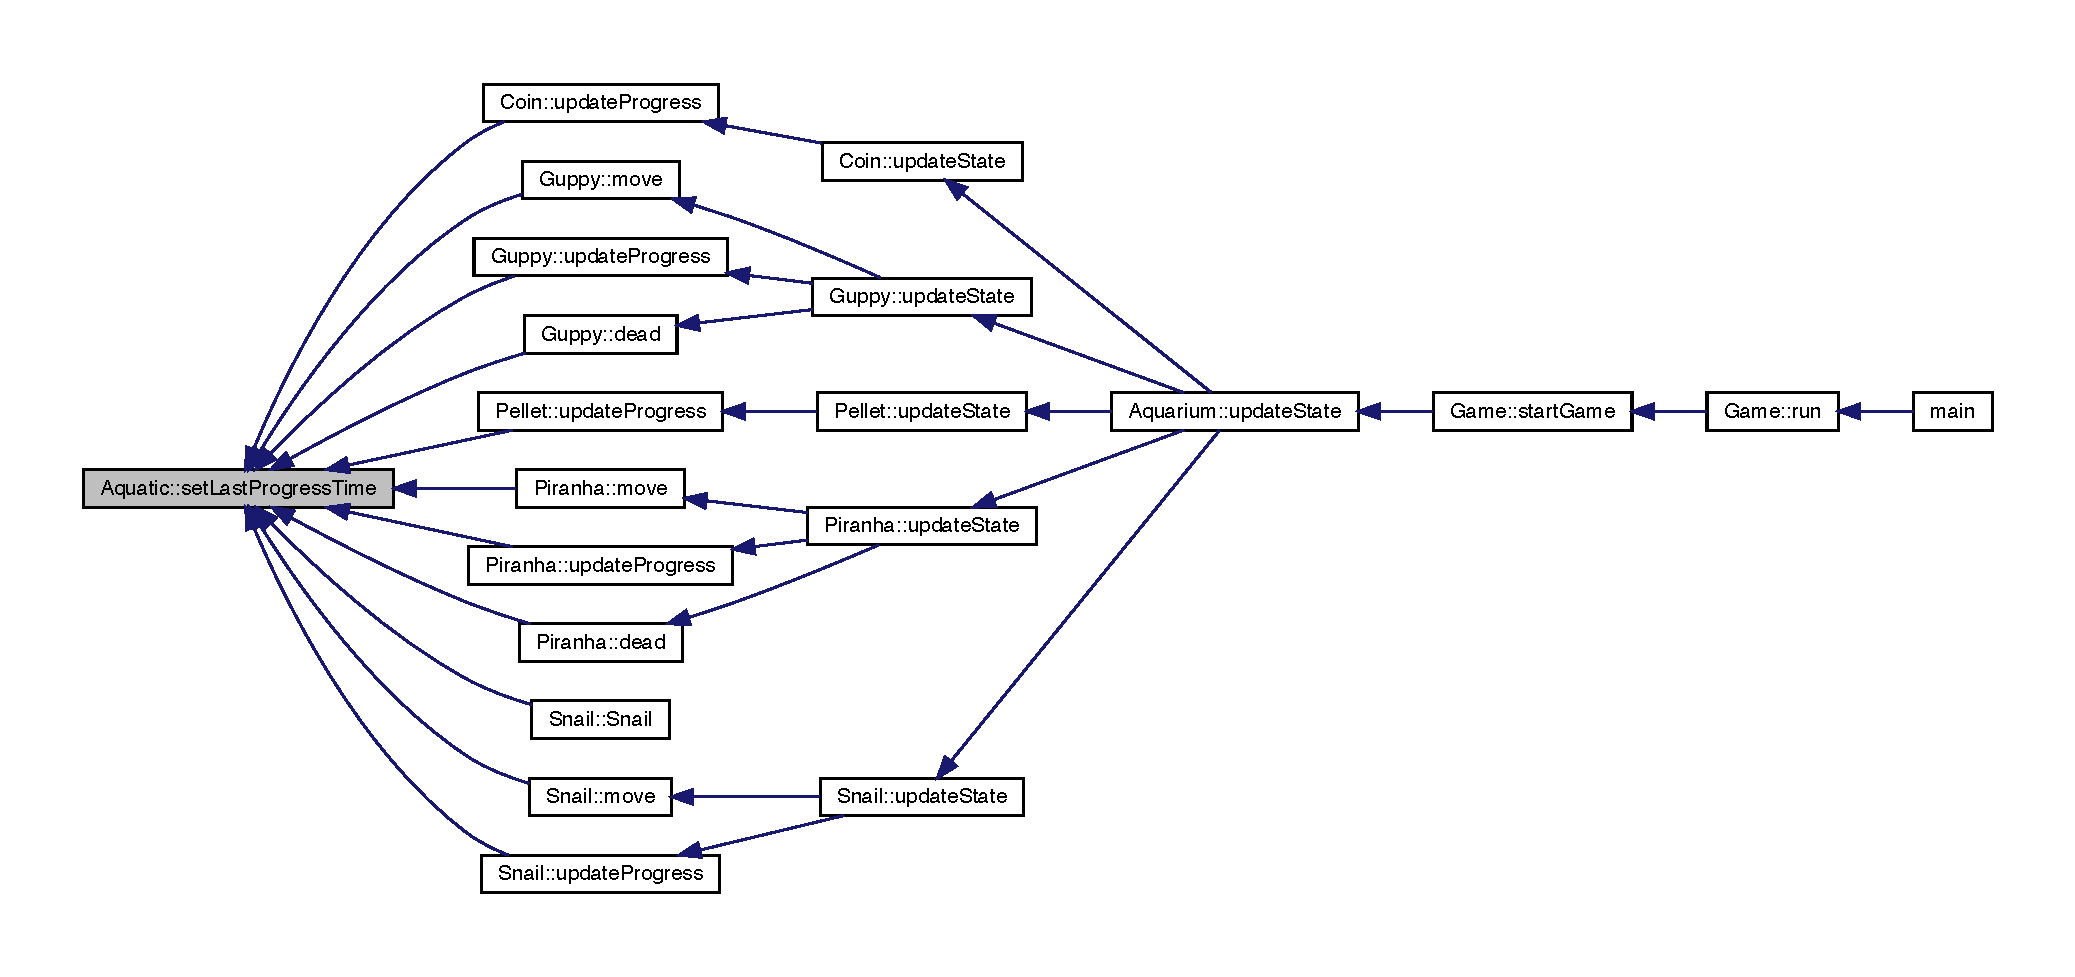
\includegraphics[width=350pt]{class_aquatic_a50e51e4b7bfd7f46d3c43bde27e0a5d8_icgraph}
\end{center}
\end{figure}
\mbox{\Hypertarget{class_aquatic_a56bd74d0814dd9ed13b395c0033eb594}\label{class_aquatic_a56bd74d0814dd9ed13b395c0033eb594}} 
\index{Aquatic@{Aquatic}!set\+Progress@{set\+Progress}}
\index{set\+Progress@{set\+Progress}!Aquatic@{Aquatic}}
\subsubsection{\texorpdfstring{set\+Progress()}{setProgress()}}
{\footnotesize\ttfamily void Aquatic\+::set\+Progress (\begin{DoxyParamCaption}\item[{int}]{progress }\end{DoxyParamCaption})}



Setter for progress. 


\begin{DoxyParams}{Parameters}
{\em int} & progress \\
\hline
\end{DoxyParams}
Here is the caller graph for this function\+:
\nopagebreak
\begin{figure}[H]
\begin{center}
\leavevmode
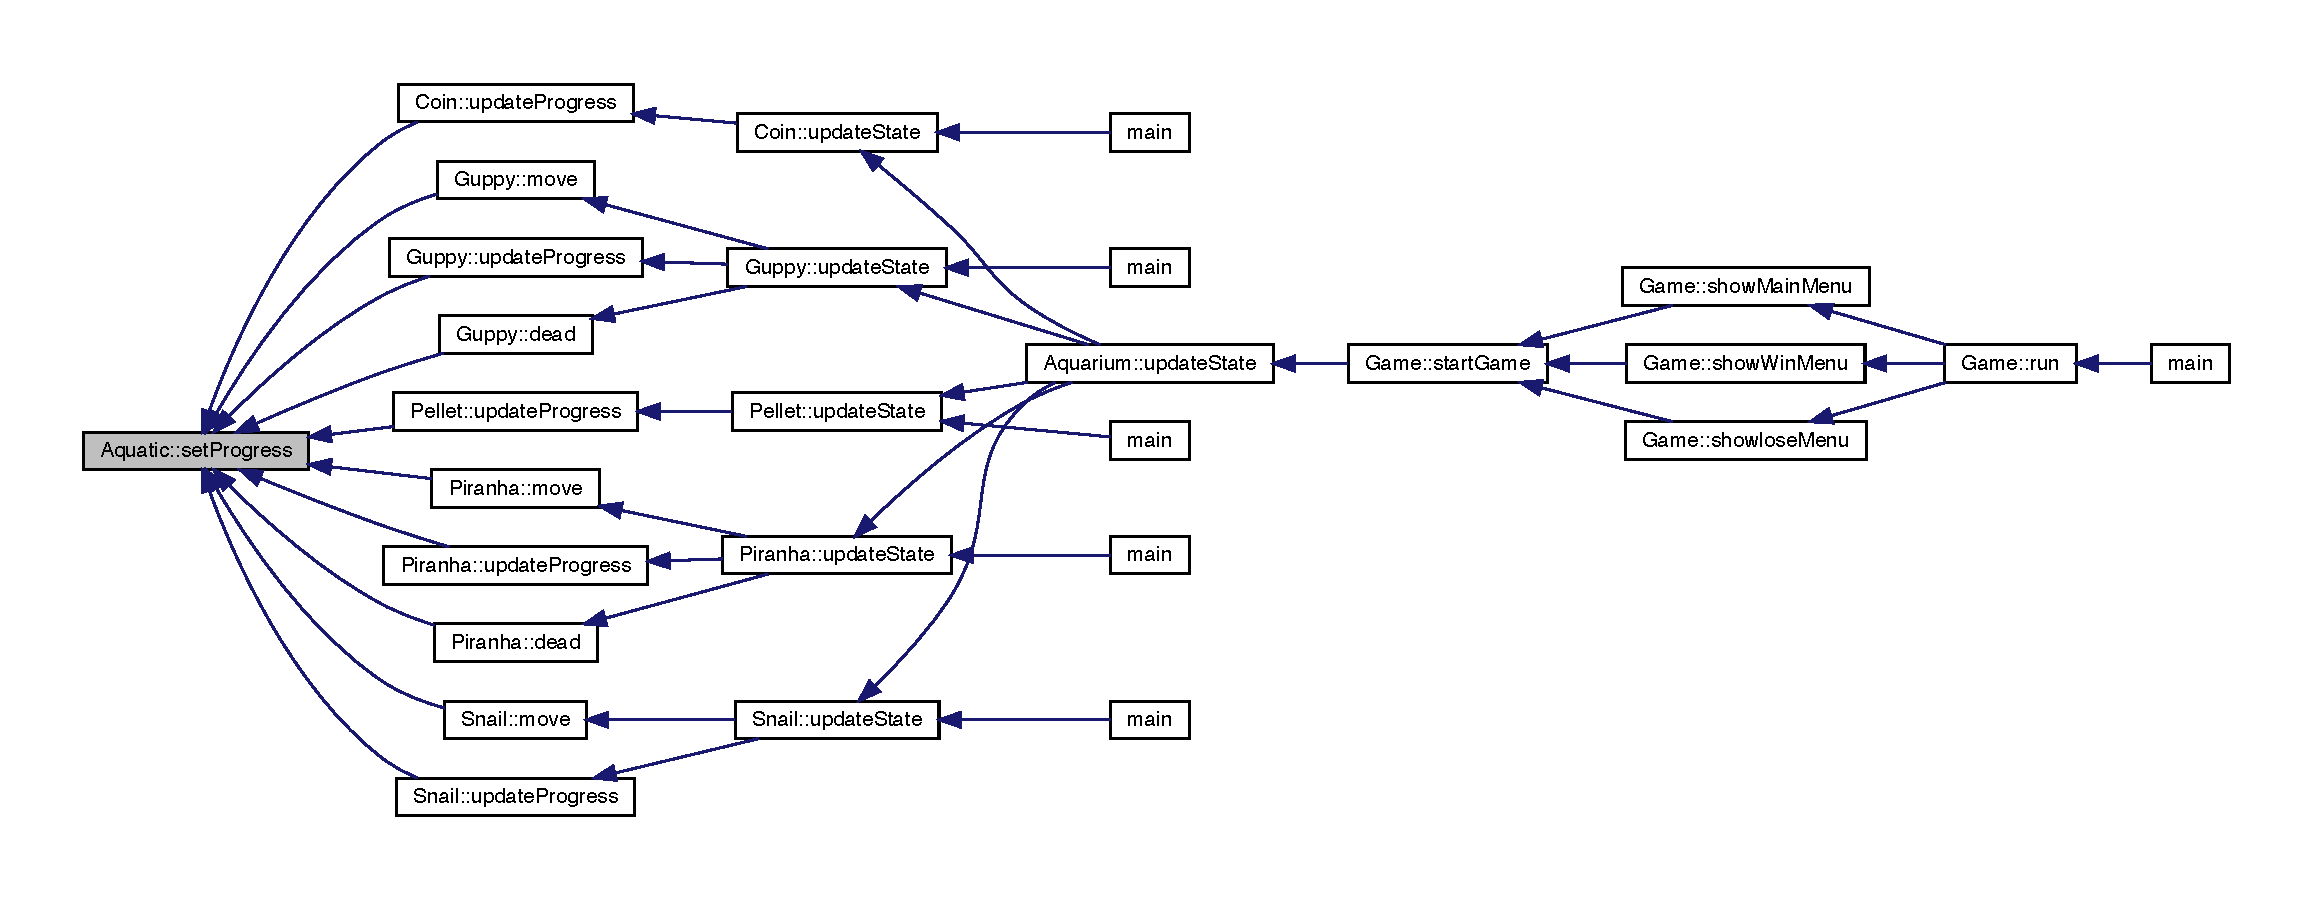
\includegraphics[width=350pt]{class_aquatic_a56bd74d0814dd9ed13b395c0033eb594_icgraph}
\end{center}
\end{figure}
\mbox{\Hypertarget{class_aquatic_a33de0f838d9a6f504cd8efeaa112b4ea}\label{class_aquatic_a33de0f838d9a6f504cd8efeaa112b4ea}} 
\index{Aquatic@{Aquatic}!set\+State@{set\+State}}
\index{set\+State@{set\+State}!Aquatic@{Aquatic}}
\subsubsection{\texorpdfstring{set\+State()}{setState()}}
{\footnotesize\ttfamily void Aquatic\+::set\+State (\begin{DoxyParamCaption}\item[{\mbox{\hyperlink{_constants_8hpp_a5d74787dedbc4e11c1ab15bf487e61f8}{State}}}]{state }\end{DoxyParamCaption})}



Setter for state. 


\begin{DoxyParams}{Parameters}
{\em State} & state \\
\hline
\end{DoxyParams}
Here is the caller graph for this function\+:
\nopagebreak
\begin{figure}[H]
\begin{center}
\leavevmode
\includegraphics[width=350pt]{class_aquatic_a33de0f838d9a6f504cd8efeaa112b4ea_icgraph}
\end{center}
\end{figure}
\mbox{\Hypertarget{class_aquatic_a4f5f9426805afd153c659cd0bb535ef6}\label{class_aquatic_a4f5f9426805afd153c659cd0bb535ef6}} 
\index{Aquatic@{Aquatic}!setX@{setX}}
\index{setX@{setX}!Aquatic@{Aquatic}}
\subsubsection{\texorpdfstring{set\+X()}{setX()}}
{\footnotesize\ttfamily void Aquatic\+::setX (\begin{DoxyParamCaption}\item[{double}]{x }\end{DoxyParamCaption})}



Setter for x. 


\begin{DoxyParams}{Parameters}
{\em double} & x \\
\hline
\end{DoxyParams}
Here is the caller graph for this function\+:
\nopagebreak
\begin{figure}[H]
\begin{center}
\leavevmode
\includegraphics[width=350pt]{class_aquatic_a4f5f9426805afd153c659cd0bb535ef6_icgraph}
\end{center}
\end{figure}
\mbox{\Hypertarget{class_aquatic_af767ef441e7112a700975f6709b85dc9}\label{class_aquatic_af767ef441e7112a700975f6709b85dc9}} 
\index{Aquatic@{Aquatic}!setY@{setY}}
\index{setY@{setY}!Aquatic@{Aquatic}}
\subsubsection{\texorpdfstring{set\+Y()}{setY()}}
{\footnotesize\ttfamily void Aquatic\+::setY (\begin{DoxyParamCaption}\item[{double}]{y }\end{DoxyParamCaption})}



Setter for y. 


\begin{DoxyParams}{Parameters}
{\em double} & y \\
\hline
\end{DoxyParams}
Here is the caller graph for this function\+:
\nopagebreak
\begin{figure}[H]
\begin{center}
\leavevmode
\includegraphics[width=350pt]{class_aquatic_af767ef441e7112a700975f6709b85dc9_icgraph}
\end{center}
\end{figure}
\mbox{\Hypertarget{class_aquatic_ae1b6301ed27d6aadb73c7ee7879c24af}\label{class_aquatic_ae1b6301ed27d6aadb73c7ee7879c24af}} 
\index{Aquatic@{Aquatic}!update\+Progress@{update\+Progress}}
\index{update\+Progress@{update\+Progress}!Aquatic@{Aquatic}}
\subsubsection{\texorpdfstring{update\+Progress()}{updateProgress()}}
{\footnotesize\ttfamily virtual void Aquatic\+::update\+Progress (\begin{DoxyParamCaption}{ }\end{DoxyParamCaption})\hspace{0.3cm}{\ttfamily [pure virtual]}}



Updates the object progress independently. 



Implemented in \mbox{\hyperlink{class_snail_a327c2d31017320c4cd18b48103905fa7}{Snail}}, \mbox{\hyperlink{class_guppy_af22eacc4a1ea7bec4be7b5d82148407b}{Guppy}}, \mbox{\hyperlink{class_piranha_ac4906080867655ef09591eba1cf2f00c}{Piranha}}, \mbox{\hyperlink{class_coin_ac54d7b690f7e415d2220711f718f638e}{Coin}}, and \mbox{\hyperlink{class_pellet_a1a7203cff52c771eb8cc62a91620e3ca}{Pellet}}.

\mbox{\Hypertarget{class_aquatic_a51e44c95476d72a841fea667c6cbbedc}\label{class_aquatic_a51e44c95476d72a841fea667c6cbbedc}} 
\index{Aquatic@{Aquatic}!update\+State@{update\+State}}
\index{update\+State@{update\+State}!Aquatic@{Aquatic}}
\subsubsection{\texorpdfstring{update\+State()}{updateState()}}
{\footnotesize\ttfamily virtual void Aquatic\+::update\+State (\begin{DoxyParamCaption}{ }\end{DoxyParamCaption})\hspace{0.3cm}{\ttfamily [pure virtual]}}



Updates the object state independently. 



Implemented in \mbox{\hyperlink{class_snail_a46dbefb10308c29341d96423e853cb2b}{Snail}}, \mbox{\hyperlink{class_guppy_ac62ef7053d40430ad98c1d5a54699f9d}{Guppy}}, \mbox{\hyperlink{class_piranha_a851c302af9de1d6eaf727242e2912f62}{Piranha}}, \mbox{\hyperlink{class_coin_ac9d03cbd68f9ccb739895832f77d60a3}{Coin}}, and \mbox{\hyperlink{class_pellet_ab21f88899eba022e1693d911eba9dbfb}{Pellet}}.



The documentation for this class was generated from the following files\+:\begin{DoxyCompactItemize}
\item 
aquatic/\mbox{\hyperlink{_aquatic_8hpp}{Aquatic.\+hpp}}\item 
aquatic/\mbox{\hyperlink{_aquatic_8cpp}{Aquatic.\+cpp}}\end{DoxyCompactItemize}

\hypertarget{class_coin}{}\section{Coin Class Reference}
\label{class_coin}\index{Coin@{Coin}}


Class \mbox{\hyperlink{class_coin}{Coin}}. Represents all \mbox{\hyperlink{class_coin}{Coin}} object in \mbox{\hyperlink{class_aquarium}{Aquarium}}.  




{\ttfamily \#include $<$Coin.\+hpp$>$}



Inheritance diagram for Coin\+:\nopagebreak
\begin{figure}[H]
\begin{center}
\leavevmode
\includegraphics[width=129pt]{class_coin__inherit__graph}
\end{center}
\end{figure}


Collaboration diagram for Coin\+:\nopagebreak
\begin{figure}[H]
\begin{center}
\leavevmode
\includegraphics[width=129pt]{class_coin__coll__graph}
\end{center}
\end{figure}
\subsection*{Public Member Functions}
\begin{DoxyCompactItemize}
\item 
\mbox{\hyperlink{class_coin_a60b7cf94d6893b82e2b450580f555e83}{Coin}} (double x, double y, int value, \mbox{\hyperlink{class_aquarium}{Aquarium}} $\ast$aquarium)
\begin{DoxyCompactList}\small\item\em A constructor. \end{DoxyCompactList}\item 
int \mbox{\hyperlink{class_coin_a53c8bf65afdde1422cfda51d753d74b7}{get\+Value}} () const
\begin{DoxyCompactList}\small\item\em Getter for value. \end{DoxyCompactList}\item 
void \mbox{\hyperlink{class_coin_ac9d03cbd68f9ccb739895832f77d60a3}{update\+State}} ()
\begin{DoxyCompactList}\small\item\em Implements pure virtual method from \mbox{\hyperlink{class_aquatic}{Aquatic}}. \end{DoxyCompactList}\item 
void \mbox{\hyperlink{class_coin_ab62bca5834489b9b483deaa3ca3470e9}{move}} ()
\begin{DoxyCompactList}\small\item\em Implements pure virtual method from \mbox{\hyperlink{class_aquatic}{Aquatic}}. \end{DoxyCompactList}\item 
void \mbox{\hyperlink{class_coin_ac54d7b690f7e415d2220711f718f638e}{update\+Progress}} ()
\begin{DoxyCompactList}\small\item\em Implements pure virtual method from \mbox{\hyperlink{class_aquatic}{Aquatic}}. \end{DoxyCompactList}\item 
void \mbox{\hyperlink{class_coin_af0c650f68a63698691c574fbef940776}{dead}} ()
\begin{DoxyCompactList}\small\item\em Implements pure virtual method from \mbox{\hyperlink{class_aquatic}{Aquatic}}. \end{DoxyCompactList}\end{DoxyCompactItemize}


\subsection{Detailed Description}
Class \mbox{\hyperlink{class_coin}{Coin}}. Represents all \mbox{\hyperlink{class_coin}{Coin}} object in \mbox{\hyperlink{class_aquarium}{Aquarium}}. 

\subsection{Constructor \& Destructor Documentation}
\mbox{\Hypertarget{class_coin_a60b7cf94d6893b82e2b450580f555e83}\label{class_coin_a60b7cf94d6893b82e2b450580f555e83}} 
\index{Coin@{Coin}!Coin@{Coin}}
\index{Coin@{Coin}!Coin@{Coin}}
\subsubsection{\texorpdfstring{Coin()}{Coin()}}
{\footnotesize\ttfamily Coin\+::\+Coin (\begin{DoxyParamCaption}\item[{double}]{x,  }\item[{double}]{y,  }\item[{int}]{value,  }\item[{\mbox{\hyperlink{class_aquarium}{Aquarium}} $\ast$}]{aquarium }\end{DoxyParamCaption})}



A constructor. 

Constructs a new \mbox{\hyperlink{class_coin}{Coin}} object. 
\begin{DoxyParams}{Parameters}
{\em double} & x x-\/axis position of the \mbox{\hyperlink{class_coin}{Coin}}. \\
\hline
{\em double} & y y-\/axis position of the \mbox{\hyperlink{class_coin}{Coin}}. \\
\hline
{\em int} & value Value of the \mbox{\hyperlink{class_coin}{Coin}}. \\
\hline
{\em \mbox{\hyperlink{class_aquarium}{Aquarium}}} & $\ast$aquarium The \mbox{\hyperlink{class_aquarium}{Aquarium}} that contains the object. \\
\hline
\end{DoxyParams}
Here is the call graph for this function\+:\nopagebreak
\begin{figure}[H]
\begin{center}
\leavevmode
\includegraphics[width=270pt]{class_coin_a60b7cf94d6893b82e2b450580f555e83_cgraph}
\end{center}
\end{figure}


\subsection{Member Function Documentation}
\mbox{\Hypertarget{class_coin_af0c650f68a63698691c574fbef940776}\label{class_coin_af0c650f68a63698691c574fbef940776}} 
\index{Coin@{Coin}!dead@{dead}}
\index{dead@{dead}!Coin@{Coin}}
\subsubsection{\texorpdfstring{dead()}{dead()}}
{\footnotesize\ttfamily void Coin\+::dead (\begin{DoxyParamCaption}{ }\end{DoxyParamCaption})\hspace{0.3cm}{\ttfamily [virtual]}}



Implements pure virtual method from \mbox{\hyperlink{class_aquatic}{Aquatic}}. 



Implements \mbox{\hyperlink{class_aquatic_a22fdb11e9cfec922fe50638709768276}{Aquatic}}.

Here is the call graph for this function\+:\nopagebreak
\begin{figure}[H]
\begin{center}
\leavevmode
\includegraphics[width=350pt]{class_coin_af0c650f68a63698691c574fbef940776_cgraph}
\end{center}
\end{figure}
Here is the caller graph for this function\+:
\nopagebreak
\begin{figure}[H]
\begin{center}
\leavevmode
\includegraphics[width=350pt]{class_coin_af0c650f68a63698691c574fbef940776_icgraph}
\end{center}
\end{figure}
\mbox{\Hypertarget{class_coin_a53c8bf65afdde1422cfda51d753d74b7}\label{class_coin_a53c8bf65afdde1422cfda51d753d74b7}} 
\index{Coin@{Coin}!get\+Value@{get\+Value}}
\index{get\+Value@{get\+Value}!Coin@{Coin}}
\subsubsection{\texorpdfstring{get\+Value()}{getValue()}}
{\footnotesize\ttfamily int Coin\+::get\+Value (\begin{DoxyParamCaption}{ }\end{DoxyParamCaption}) const}



Getter for value. 

\begin{DoxyReturn}{Returns}
int value. 
\end{DoxyReturn}
Here is the caller graph for this function\+:
\nopagebreak
\begin{figure}[H]
\begin{center}
\leavevmode
\includegraphics[width=350pt]{class_coin_a53c8bf65afdde1422cfda51d753d74b7_icgraph}
\end{center}
\end{figure}
\mbox{\Hypertarget{class_coin_ab62bca5834489b9b483deaa3ca3470e9}\label{class_coin_ab62bca5834489b9b483deaa3ca3470e9}} 
\index{Coin@{Coin}!move@{move}}
\index{move@{move}!Coin@{Coin}}
\subsubsection{\texorpdfstring{move()}{move()}}
{\footnotesize\ttfamily void Coin\+::move (\begin{DoxyParamCaption}{ }\end{DoxyParamCaption})\hspace{0.3cm}{\ttfamily [virtual]}}



Implements pure virtual method from \mbox{\hyperlink{class_aquatic}{Aquatic}}. 



Implements \mbox{\hyperlink{class_aquatic_a962e93c804814eeaf3cea6e26698eef7}{Aquatic}}.

Here is the call graph for this function\+:\nopagebreak
\begin{figure}[H]
\begin{center}
\leavevmode
\includegraphics[width=350pt]{class_coin_ab62bca5834489b9b483deaa3ca3470e9_cgraph}
\end{center}
\end{figure}
Here is the caller graph for this function\+:
\nopagebreak
\begin{figure}[H]
\begin{center}
\leavevmode
\includegraphics[width=350pt]{class_coin_ab62bca5834489b9b483deaa3ca3470e9_icgraph}
\end{center}
\end{figure}
\mbox{\Hypertarget{class_coin_ac54d7b690f7e415d2220711f718f638e}\label{class_coin_ac54d7b690f7e415d2220711f718f638e}} 
\index{Coin@{Coin}!update\+Progress@{update\+Progress}}
\index{update\+Progress@{update\+Progress}!Coin@{Coin}}
\subsubsection{\texorpdfstring{update\+Progress()}{updateProgress()}}
{\footnotesize\ttfamily void Coin\+::update\+Progress (\begin{DoxyParamCaption}{ }\end{DoxyParamCaption})\hspace{0.3cm}{\ttfamily [virtual]}}



Implements pure virtual method from \mbox{\hyperlink{class_aquatic}{Aquatic}}. 



Implements \mbox{\hyperlink{class_aquatic_ae1b6301ed27d6aadb73c7ee7879c24af}{Aquatic}}.

Here is the call graph for this function\+:\nopagebreak
\begin{figure}[H]
\begin{center}
\leavevmode
\includegraphics[width=350pt]{class_coin_ac54d7b690f7e415d2220711f718f638e_cgraph}
\end{center}
\end{figure}
Here is the caller graph for this function\+:
\nopagebreak
\begin{figure}[H]
\begin{center}
\leavevmode
\includegraphics[width=350pt]{class_coin_ac54d7b690f7e415d2220711f718f638e_icgraph}
\end{center}
\end{figure}
\mbox{\Hypertarget{class_coin_ac9d03cbd68f9ccb739895832f77d60a3}\label{class_coin_ac9d03cbd68f9ccb739895832f77d60a3}} 
\index{Coin@{Coin}!update\+State@{update\+State}}
\index{update\+State@{update\+State}!Coin@{Coin}}
\subsubsection{\texorpdfstring{update\+State()}{updateState()}}
{\footnotesize\ttfamily void Coin\+::update\+State (\begin{DoxyParamCaption}{ }\end{DoxyParamCaption})\hspace{0.3cm}{\ttfamily [virtual]}}



Implements pure virtual method from \mbox{\hyperlink{class_aquatic}{Aquatic}}. 



Implements \mbox{\hyperlink{class_aquatic_a51e44c95476d72a841fea667c6cbbedc}{Aquatic}}.

Here is the call graph for this function\+:\nopagebreak
\begin{figure}[H]
\begin{center}
\leavevmode
\includegraphics[width=350pt]{class_coin_ac9d03cbd68f9ccb739895832f77d60a3_cgraph}
\end{center}
\end{figure}
Here is the caller graph for this function\+:
\nopagebreak
\begin{figure}[H]
\begin{center}
\leavevmode
\includegraphics[width=350pt]{class_coin_ac9d03cbd68f9ccb739895832f77d60a3_icgraph}
\end{center}
\end{figure}


The documentation for this class was generated from the following files\+:\begin{DoxyCompactItemize}
\item 
coin/\mbox{\hyperlink{_coin_8hpp}{Coin.\+hpp}}\item 
coin/\mbox{\hyperlink{_coin_8cpp}{Coin.\+cpp}}\end{DoxyCompactItemize}

\hypertarget{class_fish}{}\section{Fish Class Reference}
\label{class_fish}\index{Fish@{Fish}}


Abstract Class \mbox{\hyperlink{class_fish}{Fish}}. Represents all \mbox{\hyperlink{class_fish}{Fish}} object in \mbox{\hyperlink{class_aquarium}{Aquarium}} such as \mbox{\hyperlink{class_piranha}{Piranha}} and \mbox{\hyperlink{class_guppy}{Guppy}}.  




{\ttfamily \#include $<$Fish.\+hpp$>$}



Inheritance diagram for Fish\+:\nopagebreak
\begin{figure}[H]
\begin{center}
\leavevmode
\includegraphics[width=194pt]{class_fish__inherit__graph}
\end{center}
\end{figure}
\subsection*{Public Member Functions}
\begin{DoxyCompactItemize}
\item 
\mbox{\hyperlink{class_fish_addc65c182f7c916e854b381d7d5410e3}{Fish}} (int food\+\_\+thres, double eat\+\_\+radius, double full\+\_\+interval, double hunger\+\_\+timeout, double created\+\_\+time)
\begin{DoxyCompactList}\small\item\em A constructor. \end{DoxyCompactList}\item 
double \mbox{\hyperlink{class_fish_a5cc60f7e97c95136c19d54b4e49a5262}{get\+Last\+Eat\+Time}} ()
\begin{DoxyCompactList}\small\item\em Getter for last\+\_\+eat\+\_\+time. \end{DoxyCompactList}\item 
double \mbox{\hyperlink{class_fish_a4edfa0e606e5db4a648fdd5d016e1543}{get\+Last\+Random\+Time}} ()
\begin{DoxyCompactList}\small\item\em Getter for last\+\_\+random\+\_\+time. \end{DoxyCompactList}\item 
double \mbox{\hyperlink{class_fish_ab097bcfc0f0402bc1c9e048bf2351290}{get\+Last\+Hunger\+Time}} ()
\begin{DoxyCompactList}\small\item\em Getter for last\+\_\+hunger\+\_\+time. \end{DoxyCompactList}\item 
int \mbox{\hyperlink{class_fish_a5ff6258ba2d031b4cc815e8318bea135}{get\+Food\+Eaten}} ()
\begin{DoxyCompactList}\small\item\em Getter for food\+\_\+eaten. \end{DoxyCompactList}\item 
bool \mbox{\hyperlink{class_fish_aa4f43ec5e63aff8a1db32d530a91652d}{get\+Hungry}} ()
\begin{DoxyCompactList}\small\item\em Getter for hungry. \end{DoxyCompactList}\item 
int \mbox{\hyperlink{class_fish_a3f9ad26c3d1dfbc3d1334065691d55da}{get\+Level}} ()
\begin{DoxyCompactList}\small\item\em Getter for level. \end{DoxyCompactList}\item 
void \mbox{\hyperlink{class_fish_ad53bd870836825ab0cc4b4d987325772}{set\+Last\+Eat\+Time}} (double last\+\_\+eat\+\_\+time)
\begin{DoxyCompactList}\small\item\em Setter for last\+\_\+eat\+\_\+time. \end{DoxyCompactList}\item 
void \mbox{\hyperlink{class_fish_a883d6bd47ac65d319269eee4c46cf461}{set\+Last\+Random\+Time}} (double last\+\_\+random\+\_\+time)
\begin{DoxyCompactList}\small\item\em Setter for last\+\_\+random\+\_\+time. \end{DoxyCompactList}\item 
void \mbox{\hyperlink{class_fish_aca013c7fba46ca20ab12909945e535d4}{set\+Last\+Hunger\+Time}} (double last\+\_\+hunger\+\_\+time)
\begin{DoxyCompactList}\small\item\em Setter for last\+\_\+hunger\+\_\+time. \end{DoxyCompactList}\item 
void \mbox{\hyperlink{class_fish_a37379e4c783602bd7c3d475a67167c11}{set\+Food\+Eaten}} (int food\+\_\+eaten)
\begin{DoxyCompactList}\small\item\em Setter for food\+\_\+eaten. \end{DoxyCompactList}\item 
void \mbox{\hyperlink{class_fish_a8b24063bf538f0502cf38ce5859aec8e}{set\+Hungry}} (bool hungry)
\begin{DoxyCompactList}\small\item\em Setter for hungry. \end{DoxyCompactList}\item 
void \mbox{\hyperlink{class_fish_aee737597ff02a50486c6e2096ccc220d}{set\+Level}} (int level)
\begin{DoxyCompactList}\small\item\em Setter for level. \end{DoxyCompactList}\item 
virtual void \mbox{\hyperlink{class_fish_af209980bd39b8de9b4bb38b7ad4edd04}{eat}} ()=0
\begin{DoxyCompactList}\small\item\em Eat object. \end{DoxyCompactList}\item 
virtual void \mbox{\hyperlink{class_fish_a899c7712639756297b9205e8bbcc2cf6}{drop\+Coin}} ()=0
\begin{DoxyCompactList}\small\item\em Drop coin. \end{DoxyCompactList}\end{DoxyCompactItemize}
\subsection*{Protected Attributes}
\begin{DoxyCompactItemize}
\item 
const int \mbox{\hyperlink{class_fish_aea009e0f3f93e7a728294e30f1f350ed}{food\+Thres}}
\begin{DoxyCompactList}\small\item\em Food needed for growth. \end{DoxyCompactList}\item 
const double \mbox{\hyperlink{class_fish_a51d4f0f3965f1547344559f861b907f6}{eat\+Radius}}
\begin{DoxyCompactList}\small\item\em \mbox{\hyperlink{class_pellet}{Pellet}} fetch radius. \end{DoxyCompactList}\item 
const double \mbox{\hyperlink{class_fish_a1a98bca18c072e53bfcb27203aac5665}{full\+Interval}}
\begin{DoxyCompactList}\small\item\em Duration until next hunger. \end{DoxyCompactList}\item 
const double \mbox{\hyperlink{class_fish_aa8090ae6de19904c27d039fc28691da7}{hunger\+Timeout}}
\begin{DoxyCompactList}\small\item\em Duration until starvation. \end{DoxyCompactList}\item 
double \mbox{\hyperlink{class_fish_af2d14945a447d890696f16ac60a43b4a}{x\+\_\+dir}}
\begin{DoxyCompactList}\small\item\em X-\/axis direction of the \mbox{\hyperlink{class_fish}{Fish}}. \end{DoxyCompactList}\item 
double \mbox{\hyperlink{class_fish_a5e9e0091482ec1bdf758fd5947564ac7}{y\+\_\+dir}}
\begin{DoxyCompactList}\small\item\em Y-\/axis direction of the \mbox{\hyperlink{class_fish}{Fish}}. \end{DoxyCompactList}\end{DoxyCompactItemize}


\subsection{Detailed Description}
Abstract Class \mbox{\hyperlink{class_fish}{Fish}}. Represents all \mbox{\hyperlink{class_fish}{Fish}} object in \mbox{\hyperlink{class_aquarium}{Aquarium}} such as \mbox{\hyperlink{class_piranha}{Piranha}} and \mbox{\hyperlink{class_guppy}{Guppy}}. 

\subsection{Constructor \& Destructor Documentation}
\mbox{\Hypertarget{class_fish_addc65c182f7c916e854b381d7d5410e3}\label{class_fish_addc65c182f7c916e854b381d7d5410e3}} 
\index{Fish@{Fish}!Fish@{Fish}}
\index{Fish@{Fish}!Fish@{Fish}}
\subsubsection{\texorpdfstring{Fish()}{Fish()}}
{\footnotesize\ttfamily Fish\+::\+Fish (\begin{DoxyParamCaption}\item[{int}]{food\+\_\+thres,  }\item[{double}]{eat\+\_\+radius,  }\item[{double}]{full\+\_\+interval,  }\item[{double}]{hunger\+\_\+timeout,  }\item[{double}]{created\+\_\+time }\end{DoxyParamCaption})}



A constructor. 

Constructs a new \mbox{\hyperlink{class_fish}{Fish}} object. 
\begin{DoxyParams}{Parameters}
{\em int} & food\+\_\+thres Number of food to level up. \\
\hline
{\em double} & eat\+\_\+radius \\
\hline
{\em double} & full\+\_\+interval Full to hungry interval. \\
\hline
{\em double} & hunger\+\_\+timeout Hungry to dead interval if there\textquotesingle{}s no food. \\
\hline
{\em double} & created\+\_\+time \\
\hline
\end{DoxyParams}


\subsection{Member Function Documentation}
\mbox{\Hypertarget{class_fish_a899c7712639756297b9205e8bbcc2cf6}\label{class_fish_a899c7712639756297b9205e8bbcc2cf6}} 
\index{Fish@{Fish}!drop\+Coin@{drop\+Coin}}
\index{drop\+Coin@{drop\+Coin}!Fish@{Fish}}
\subsubsection{\texorpdfstring{drop\+Coin()}{dropCoin()}}
{\footnotesize\ttfamily virtual void Fish\+::drop\+Coin (\begin{DoxyParamCaption}{ }\end{DoxyParamCaption})\hspace{0.3cm}{\ttfamily [pure virtual]}}



Drop coin. 

Drop coin following each subclasses rule 

Implemented in \mbox{\hyperlink{class_guppy_a356d1f45f52684bba3e6e9e7774e59b8}{Guppy}}, and \mbox{\hyperlink{class_piranha_aee107987f36631002f04c5283564382b}{Piranha}}.

\mbox{\Hypertarget{class_fish_af209980bd39b8de9b4bb38b7ad4edd04}\label{class_fish_af209980bd39b8de9b4bb38b7ad4edd04}} 
\index{Fish@{Fish}!eat@{eat}}
\index{eat@{eat}!Fish@{Fish}}
\subsubsection{\texorpdfstring{eat()}{eat()}}
{\footnotesize\ttfamily virtual void Fish\+::eat (\begin{DoxyParamCaption}{ }\end{DoxyParamCaption})\hspace{0.3cm}{\ttfamily [pure virtual]}}



Eat object. 

Eat food if the food is in range 

Implemented in \mbox{\hyperlink{class_guppy_afe934262a0988e4ad041f4ed3a1a7e02}{Guppy}}, and \mbox{\hyperlink{class_piranha_ac48c0256edd56c427b3d82f6e0d4df82}{Piranha}}.

\mbox{\Hypertarget{class_fish_a5ff6258ba2d031b4cc815e8318bea135}\label{class_fish_a5ff6258ba2d031b4cc815e8318bea135}} 
\index{Fish@{Fish}!get\+Food\+Eaten@{get\+Food\+Eaten}}
\index{get\+Food\+Eaten@{get\+Food\+Eaten}!Fish@{Fish}}
\subsubsection{\texorpdfstring{get\+Food\+Eaten()}{getFoodEaten()}}
{\footnotesize\ttfamily int Fish\+::get\+Food\+Eaten (\begin{DoxyParamCaption}{ }\end{DoxyParamCaption})}



Getter for food\+\_\+eaten. 

\begin{DoxyReturn}{Returns}
int food\+\_\+eaten Number of food eaten. 
\end{DoxyReturn}
Here is the caller graph for this function\+:
\nopagebreak
\begin{figure}[H]
\begin{center}
\leavevmode
\includegraphics[width=350pt]{class_fish_a5ff6258ba2d031b4cc815e8318bea135_icgraph}
\end{center}
\end{figure}
\mbox{\Hypertarget{class_fish_aa4f43ec5e63aff8a1db32d530a91652d}\label{class_fish_aa4f43ec5e63aff8a1db32d530a91652d}} 
\index{Fish@{Fish}!get\+Hungry@{get\+Hungry}}
\index{get\+Hungry@{get\+Hungry}!Fish@{Fish}}
\subsubsection{\texorpdfstring{get\+Hungry()}{getHungry()}}
{\footnotesize\ttfamily bool Fish\+::get\+Hungry (\begin{DoxyParamCaption}{ }\end{DoxyParamCaption})}



Getter for hungry. 

\begin{DoxyReturn}{Returns}
bool hungry status of the \mbox{\hyperlink{class_fish}{Fish}}. 
\end{DoxyReturn}
Here is the caller graph for this function\+:
\nopagebreak
\begin{figure}[H]
\begin{center}
\leavevmode
\includegraphics[width=350pt]{class_fish_aa4f43ec5e63aff8a1db32d530a91652d_icgraph}
\end{center}
\end{figure}
\mbox{\Hypertarget{class_fish_a5cc60f7e97c95136c19d54b4e49a5262}\label{class_fish_a5cc60f7e97c95136c19d54b4e49a5262}} 
\index{Fish@{Fish}!get\+Last\+Eat\+Time@{get\+Last\+Eat\+Time}}
\index{get\+Last\+Eat\+Time@{get\+Last\+Eat\+Time}!Fish@{Fish}}
\subsubsection{\texorpdfstring{get\+Last\+Eat\+Time()}{getLastEatTime()}}
{\footnotesize\ttfamily double Fish\+::get\+Last\+Eat\+Time (\begin{DoxyParamCaption}{ }\end{DoxyParamCaption})}



Getter for last\+\_\+eat\+\_\+time. 

\begin{DoxyReturn}{Returns}
double last\+\_\+eat\+\_\+time 
\end{DoxyReturn}
Here is the caller graph for this function\+:
\nopagebreak
\begin{figure}[H]
\begin{center}
\leavevmode
\includegraphics[width=350pt]{class_fish_a5cc60f7e97c95136c19d54b4e49a5262_icgraph}
\end{center}
\end{figure}
\mbox{\Hypertarget{class_fish_ab097bcfc0f0402bc1c9e048bf2351290}\label{class_fish_ab097bcfc0f0402bc1c9e048bf2351290}} 
\index{Fish@{Fish}!get\+Last\+Hunger\+Time@{get\+Last\+Hunger\+Time}}
\index{get\+Last\+Hunger\+Time@{get\+Last\+Hunger\+Time}!Fish@{Fish}}
\subsubsection{\texorpdfstring{get\+Last\+Hunger\+Time()}{getLastHungerTime()}}
{\footnotesize\ttfamily double Fish\+::get\+Last\+Hunger\+Time (\begin{DoxyParamCaption}{ }\end{DoxyParamCaption})}



Getter for last\+\_\+hunger\+\_\+time. 

\begin{DoxyReturn}{Returns}
double last\+\_\+hunger\+\_\+time 
\end{DoxyReturn}
Here is the caller graph for this function\+:
\nopagebreak
\begin{figure}[H]
\begin{center}
\leavevmode
\includegraphics[width=350pt]{class_fish_ab097bcfc0f0402bc1c9e048bf2351290_icgraph}
\end{center}
\end{figure}
\mbox{\Hypertarget{class_fish_a4edfa0e606e5db4a648fdd5d016e1543}\label{class_fish_a4edfa0e606e5db4a648fdd5d016e1543}} 
\index{Fish@{Fish}!get\+Last\+Random\+Time@{get\+Last\+Random\+Time}}
\index{get\+Last\+Random\+Time@{get\+Last\+Random\+Time}!Fish@{Fish}}
\subsubsection{\texorpdfstring{get\+Last\+Random\+Time()}{getLastRandomTime()}}
{\footnotesize\ttfamily double Fish\+::get\+Last\+Random\+Time (\begin{DoxyParamCaption}{ }\end{DoxyParamCaption})}



Getter for last\+\_\+random\+\_\+time. 

\begin{DoxyReturn}{Returns}
double last\+\_\+random\+\_\+time 
\end{DoxyReturn}
Here is the caller graph for this function\+:
\nopagebreak
\begin{figure}[H]
\begin{center}
\leavevmode
\includegraphics[width=350pt]{class_fish_a4edfa0e606e5db4a648fdd5d016e1543_icgraph}
\end{center}
\end{figure}
\mbox{\Hypertarget{class_fish_a3f9ad26c3d1dfbc3d1334065691d55da}\label{class_fish_a3f9ad26c3d1dfbc3d1334065691d55da}} 
\index{Fish@{Fish}!get\+Level@{get\+Level}}
\index{get\+Level@{get\+Level}!Fish@{Fish}}
\subsubsection{\texorpdfstring{get\+Level()}{getLevel()}}
{\footnotesize\ttfamily int Fish\+::get\+Level (\begin{DoxyParamCaption}{ }\end{DoxyParamCaption})}



Getter for level. 

\begin{DoxyReturn}{Returns}
int level of the \mbox{\hyperlink{class_fish}{Fish}}. 
\end{DoxyReturn}
Here is the caller graph for this function\+:
\nopagebreak
\begin{figure}[H]
\begin{center}
\leavevmode
\includegraphics[width=350pt]{class_fish_a3f9ad26c3d1dfbc3d1334065691d55da_icgraph}
\end{center}
\end{figure}
\mbox{\Hypertarget{class_fish_a37379e4c783602bd7c3d475a67167c11}\label{class_fish_a37379e4c783602bd7c3d475a67167c11}} 
\index{Fish@{Fish}!set\+Food\+Eaten@{set\+Food\+Eaten}}
\index{set\+Food\+Eaten@{set\+Food\+Eaten}!Fish@{Fish}}
\subsubsection{\texorpdfstring{set\+Food\+Eaten()}{setFoodEaten()}}
{\footnotesize\ttfamily void Fish\+::set\+Food\+Eaten (\begin{DoxyParamCaption}\item[{int}]{food\+\_\+eaten }\end{DoxyParamCaption})}



Setter for food\+\_\+eaten. 


\begin{DoxyParams}{Parameters}
{\em int} & food\+\_\+eaten \\
\hline
\end{DoxyParams}
Here is the caller graph for this function\+:
\nopagebreak
\begin{figure}[H]
\begin{center}
\leavevmode
\includegraphics[width=350pt]{class_fish_a37379e4c783602bd7c3d475a67167c11_icgraph}
\end{center}
\end{figure}
\mbox{\Hypertarget{class_fish_a8b24063bf538f0502cf38ce5859aec8e}\label{class_fish_a8b24063bf538f0502cf38ce5859aec8e}} 
\index{Fish@{Fish}!set\+Hungry@{set\+Hungry}}
\index{set\+Hungry@{set\+Hungry}!Fish@{Fish}}
\subsubsection{\texorpdfstring{set\+Hungry()}{setHungry()}}
{\footnotesize\ttfamily void Fish\+::set\+Hungry (\begin{DoxyParamCaption}\item[{bool}]{hungry }\end{DoxyParamCaption})}



Setter for hungry. 


\begin{DoxyParams}{Parameters}
{\em bool} & hungry \\
\hline
\end{DoxyParams}
Here is the caller graph for this function\+:
\nopagebreak
\begin{figure}[H]
\begin{center}
\leavevmode
\includegraphics[width=350pt]{class_fish_a8b24063bf538f0502cf38ce5859aec8e_icgraph}
\end{center}
\end{figure}
\mbox{\Hypertarget{class_fish_ad53bd870836825ab0cc4b4d987325772}\label{class_fish_ad53bd870836825ab0cc4b4d987325772}} 
\index{Fish@{Fish}!set\+Last\+Eat\+Time@{set\+Last\+Eat\+Time}}
\index{set\+Last\+Eat\+Time@{set\+Last\+Eat\+Time}!Fish@{Fish}}
\subsubsection{\texorpdfstring{set\+Last\+Eat\+Time()}{setLastEatTime()}}
{\footnotesize\ttfamily void Fish\+::set\+Last\+Eat\+Time (\begin{DoxyParamCaption}\item[{double}]{last\+\_\+eat\+\_\+time }\end{DoxyParamCaption})}



Setter for last\+\_\+eat\+\_\+time. 


\begin{DoxyParams}{Parameters}
{\em double} & last\+\_\+eat\+\_\+time \\
\hline
\end{DoxyParams}
Here is the caller graph for this function\+:
\nopagebreak
\begin{figure}[H]
\begin{center}
\leavevmode
\includegraphics[width=350pt]{class_fish_ad53bd870836825ab0cc4b4d987325772_icgraph}
\end{center}
\end{figure}
\mbox{\Hypertarget{class_fish_aca013c7fba46ca20ab12909945e535d4}\label{class_fish_aca013c7fba46ca20ab12909945e535d4}} 
\index{Fish@{Fish}!set\+Last\+Hunger\+Time@{set\+Last\+Hunger\+Time}}
\index{set\+Last\+Hunger\+Time@{set\+Last\+Hunger\+Time}!Fish@{Fish}}
\subsubsection{\texorpdfstring{set\+Last\+Hunger\+Time()}{setLastHungerTime()}}
{\footnotesize\ttfamily void Fish\+::set\+Last\+Hunger\+Time (\begin{DoxyParamCaption}\item[{double}]{last\+\_\+hunger\+\_\+time }\end{DoxyParamCaption})}



Setter for last\+\_\+hunger\+\_\+time. 


\begin{DoxyParams}{Parameters}
{\em double} & last\+\_\+hunger\+\_\+time \\
\hline
\end{DoxyParams}
Here is the caller graph for this function\+:
\nopagebreak
\begin{figure}[H]
\begin{center}
\leavevmode
\includegraphics[width=350pt]{class_fish_aca013c7fba46ca20ab12909945e535d4_icgraph}
\end{center}
\end{figure}
\mbox{\Hypertarget{class_fish_a883d6bd47ac65d319269eee4c46cf461}\label{class_fish_a883d6bd47ac65d319269eee4c46cf461}} 
\index{Fish@{Fish}!set\+Last\+Random\+Time@{set\+Last\+Random\+Time}}
\index{set\+Last\+Random\+Time@{set\+Last\+Random\+Time}!Fish@{Fish}}
\subsubsection{\texorpdfstring{set\+Last\+Random\+Time()}{setLastRandomTime()}}
{\footnotesize\ttfamily void Fish\+::set\+Last\+Random\+Time (\begin{DoxyParamCaption}\item[{double}]{last\+\_\+random\+\_\+time }\end{DoxyParamCaption})}



Setter for last\+\_\+random\+\_\+time. 


\begin{DoxyParams}{Parameters}
{\em double} & last\+\_\+random\+\_\+time \\
\hline
\end{DoxyParams}
Here is the caller graph for this function\+:
\nopagebreak
\begin{figure}[H]
\begin{center}
\leavevmode
\includegraphics[width=350pt]{class_fish_a883d6bd47ac65d319269eee4c46cf461_icgraph}
\end{center}
\end{figure}
\mbox{\Hypertarget{class_fish_aee737597ff02a50486c6e2096ccc220d}\label{class_fish_aee737597ff02a50486c6e2096ccc220d}} 
\index{Fish@{Fish}!set\+Level@{set\+Level}}
\index{set\+Level@{set\+Level}!Fish@{Fish}}
\subsubsection{\texorpdfstring{set\+Level()}{setLevel()}}
{\footnotesize\ttfamily void Fish\+::set\+Level (\begin{DoxyParamCaption}\item[{int}]{level }\end{DoxyParamCaption})}



Setter for level. 


\begin{DoxyParams}{Parameters}
{\em int} & level \\
\hline
\end{DoxyParams}
Here is the caller graph for this function\+:
\nopagebreak
\begin{figure}[H]
\begin{center}
\leavevmode
\includegraphics[width=350pt]{class_fish_aee737597ff02a50486c6e2096ccc220d_icgraph}
\end{center}
\end{figure}


\subsection{Member Data Documentation}
\mbox{\Hypertarget{class_fish_a51d4f0f3965f1547344559f861b907f6}\label{class_fish_a51d4f0f3965f1547344559f861b907f6}} 
\index{Fish@{Fish}!eat\+Radius@{eat\+Radius}}
\index{eat\+Radius@{eat\+Radius}!Fish@{Fish}}
\subsubsection{\texorpdfstring{eat\+Radius}{eatRadius}}
{\footnotesize\ttfamily const double Fish\+::eat\+Radius\hspace{0.3cm}{\ttfamily [protected]}}



\mbox{\hyperlink{class_pellet}{Pellet}} fetch radius. 

\mbox{\Hypertarget{class_fish_aea009e0f3f93e7a728294e30f1f350ed}\label{class_fish_aea009e0f3f93e7a728294e30f1f350ed}} 
\index{Fish@{Fish}!food\+Thres@{food\+Thres}}
\index{food\+Thres@{food\+Thres}!Fish@{Fish}}
\subsubsection{\texorpdfstring{food\+Thres}{foodThres}}
{\footnotesize\ttfamily const int Fish\+::food\+Thres\hspace{0.3cm}{\ttfamily [protected]}}



Food needed for growth. 

\mbox{\Hypertarget{class_fish_a1a98bca18c072e53bfcb27203aac5665}\label{class_fish_a1a98bca18c072e53bfcb27203aac5665}} 
\index{Fish@{Fish}!full\+Interval@{full\+Interval}}
\index{full\+Interval@{full\+Interval}!Fish@{Fish}}
\subsubsection{\texorpdfstring{full\+Interval}{fullInterval}}
{\footnotesize\ttfamily const double Fish\+::full\+Interval\hspace{0.3cm}{\ttfamily [protected]}}



Duration until next hunger. 

\mbox{\Hypertarget{class_fish_aa8090ae6de19904c27d039fc28691da7}\label{class_fish_aa8090ae6de19904c27d039fc28691da7}} 
\index{Fish@{Fish}!hunger\+Timeout@{hunger\+Timeout}}
\index{hunger\+Timeout@{hunger\+Timeout}!Fish@{Fish}}
\subsubsection{\texorpdfstring{hunger\+Timeout}{hungerTimeout}}
{\footnotesize\ttfamily const double Fish\+::hunger\+Timeout\hspace{0.3cm}{\ttfamily [protected]}}



Duration until starvation. 

\mbox{\Hypertarget{class_fish_af2d14945a447d890696f16ac60a43b4a}\label{class_fish_af2d14945a447d890696f16ac60a43b4a}} 
\index{Fish@{Fish}!x\+\_\+dir@{x\+\_\+dir}}
\index{x\+\_\+dir@{x\+\_\+dir}!Fish@{Fish}}
\subsubsection{\texorpdfstring{x\+\_\+dir}{x\_dir}}
{\footnotesize\ttfamily double Fish\+::x\+\_\+dir\hspace{0.3cm}{\ttfamily [protected]}}



X-\/axis direction of the \mbox{\hyperlink{class_fish}{Fish}}. 

\mbox{\Hypertarget{class_fish_a5e9e0091482ec1bdf758fd5947564ac7}\label{class_fish_a5e9e0091482ec1bdf758fd5947564ac7}} 
\index{Fish@{Fish}!y\+\_\+dir@{y\+\_\+dir}}
\index{y\+\_\+dir@{y\+\_\+dir}!Fish@{Fish}}
\subsubsection{\texorpdfstring{y\+\_\+dir}{y\_dir}}
{\footnotesize\ttfamily double Fish\+::y\+\_\+dir\hspace{0.3cm}{\ttfamily [protected]}}



Y-\/axis direction of the \mbox{\hyperlink{class_fish}{Fish}}. 



The documentation for this class was generated from the following files\+:\begin{DoxyCompactItemize}
\item 
fish/\mbox{\hyperlink{_fish_8hpp}{Fish.\+hpp}}\item 
fish/\mbox{\hyperlink{_fish_8cpp}{Fish.\+cpp}}\end{DoxyCompactItemize}

\hypertarget{class_game}{}\section{Game Class Reference}
\label{class_game}\index{Game@{Game}}


Class \mbox{\hyperlink{class_game}{Game}}. Control the game state and synchronize the game object state.  




{\ttfamily \#include $<$Game.\+hpp$>$}

\subsection*{Public Member Functions}
\begin{DoxyCompactItemize}
\item 
\mbox{\hyperlink{class_game_ad59df6562a58a614fda24622d3715b65}{Game}} ()
\begin{DoxyCompactList}\small\item\em A constructor. \end{DoxyCompactList}\item 
\mbox{\hyperlink{class_game_ae3d112ca6e0e55150d2fdbc704474530}{$\sim$\+Game}} ()
\begin{DoxyCompactList}\small\item\em A destructor. \end{DoxyCompactList}\item 
void \mbox{\hyperlink{class_game_a741532226fb50fd8113b0e2a0f162858}{init\+State}} ()
\begin{DoxyCompactList}\small\item\em Initialize game state. \end{DoxyCompactList}\item 
void \mbox{\hyperlink{class_game_a89e4124211cd2158244b9860b46c4767}{load\+State}} (string filename)
\begin{DoxyCompactList}\small\item\em Load game state from an external file. \end{DoxyCompactList}\item 
void \mbox{\hyperlink{class_game_a1d537d2349fb33959018a02eccea1c79}{save\+State}} (string filename)
\begin{DoxyCompactList}\small\item\em Save game state to an external file. \end{DoxyCompactList}\item 
void \mbox{\hyperlink{class_game_ae8638ccdb0ef3bf39a6affa30aa1258f}{start\+Game}} ()
\begin{DoxyCompactList}\small\item\em Start the game. \end{DoxyCompactList}\item 
void \mbox{\hyperlink{class_game_a1ab78f5ed0d5ea879157357cf2fb2afa}{run}} ()
\begin{DoxyCompactList}\small\item\em Run game sequence. \end{DoxyCompactList}\end{DoxyCompactItemize}


\subsection{Detailed Description}
Class \mbox{\hyperlink{class_game}{Game}}. Control the game state and synchronize the game object state. 

\subsection{Constructor \& Destructor Documentation}
\mbox{\Hypertarget{class_game_ad59df6562a58a614fda24622d3715b65}\label{class_game_ad59df6562a58a614fda24622d3715b65}} 
\index{Game@{Game}!Game@{Game}}
\index{Game@{Game}!Game@{Game}}
\subsubsection{\texorpdfstring{Game()}{Game()}}
{\footnotesize\ttfamily Game\+::\+Game (\begin{DoxyParamCaption}{ }\end{DoxyParamCaption})}



A constructor. 

Constructs a new \mbox{\hyperlink{class_game}{Game}} object. Here is the call graph for this function\+:
\nopagebreak
\begin{figure}[H]
\begin{center}
\leavevmode
\includegraphics[width=266pt]{class_game_ad59df6562a58a614fda24622d3715b65_cgraph}
\end{center}
\end{figure}
\mbox{\Hypertarget{class_game_ae3d112ca6e0e55150d2fdbc704474530}\label{class_game_ae3d112ca6e0e55150d2fdbc704474530}} 
\index{Game@{Game}!````~Game@{$\sim$\+Game}}
\index{````~Game@{$\sim$\+Game}!Game@{Game}}
\subsubsection{\texorpdfstring{$\sim$\+Game()}{~Game()}}
{\footnotesize\ttfamily Game\+::$\sim$\+Game (\begin{DoxyParamCaption}{ }\end{DoxyParamCaption})}



A destructor. 

Destructs the \mbox{\hyperlink{class_game}{Game}} object. Here is the call graph for this function\+:
\nopagebreak
\begin{figure}[H]
\begin{center}
\leavevmode
\includegraphics[width=283pt]{class_game_ae3d112ca6e0e55150d2fdbc704474530_cgraph}
\end{center}
\end{figure}


\subsection{Member Function Documentation}
\mbox{\Hypertarget{class_game_a741532226fb50fd8113b0e2a0f162858}\label{class_game_a741532226fb50fd8113b0e2a0f162858}} 
\index{Game@{Game}!init\+State@{init\+State}}
\index{init\+State@{init\+State}!Game@{Game}}
\subsubsection{\texorpdfstring{init\+State()}{initState()}}
{\footnotesize\ttfamily void Game\+::init\+State (\begin{DoxyParamCaption}{ }\end{DoxyParamCaption})}



Initialize game state. 

Here is the call graph for this function\+:\nopagebreak
\begin{figure}[H]
\begin{center}
\leavevmode
\includegraphics[width=328pt]{class_game_a741532226fb50fd8113b0e2a0f162858_cgraph}
\end{center}
\end{figure}
Here is the caller graph for this function\+:\nopagebreak
\begin{figure}[H]
\begin{center}
\leavevmode
\includegraphics[width=338pt]{class_game_a741532226fb50fd8113b0e2a0f162858_icgraph}
\end{center}
\end{figure}
\mbox{\Hypertarget{class_game_a89e4124211cd2158244b9860b46c4767}\label{class_game_a89e4124211cd2158244b9860b46c4767}} 
\index{Game@{Game}!load\+State@{load\+State}}
\index{load\+State@{load\+State}!Game@{Game}}
\subsubsection{\texorpdfstring{load\+State()}{loadState()}}
{\footnotesize\ttfamily void Game\+::load\+State (\begin{DoxyParamCaption}\item[{string}]{filename }\end{DoxyParamCaption})}



Load game state from an external file. 


\begin{DoxyParams}{Parameters}
{\em string} & filename \\
\hline
\end{DoxyParams}
\mbox{\Hypertarget{class_game_a1ab78f5ed0d5ea879157357cf2fb2afa}\label{class_game_a1ab78f5ed0d5ea879157357cf2fb2afa}} 
\index{Game@{Game}!run@{run}}
\index{run@{run}!Game@{Game}}
\subsubsection{\texorpdfstring{run()}{run()}}
{\footnotesize\ttfamily void Game\+::run (\begin{DoxyParamCaption}{ }\end{DoxyParamCaption})}



Run game sequence. 

Here is the call graph for this function\+:\nopagebreak
\begin{figure}[H]
\begin{center}
\leavevmode
\includegraphics[height=550pt]{class_game_a1ab78f5ed0d5ea879157357cf2fb2afa_cgraph}
\end{center}
\end{figure}
Here is the caller graph for this function\+:\nopagebreak
\begin{figure}[H]
\begin{center}
\leavevmode
\includegraphics[width=217pt]{class_game_a1ab78f5ed0d5ea879157357cf2fb2afa_icgraph}
\end{center}
\end{figure}
\mbox{\Hypertarget{class_game_a1d537d2349fb33959018a02eccea1c79}\label{class_game_a1d537d2349fb33959018a02eccea1c79}} 
\index{Game@{Game}!save\+State@{save\+State}}
\index{save\+State@{save\+State}!Game@{Game}}
\subsubsection{\texorpdfstring{save\+State()}{saveState()}}
{\footnotesize\ttfamily void Game\+::save\+State (\begin{DoxyParamCaption}\item[{string}]{filename }\end{DoxyParamCaption})}



Save game state to an external file. 


\begin{DoxyParams}{Parameters}
{\em string} & filename \\
\hline
\end{DoxyParams}
\mbox{\Hypertarget{class_game_ae8638ccdb0ef3bf39a6affa30aa1258f}\label{class_game_ae8638ccdb0ef3bf39a6affa30aa1258f}} 
\index{Game@{Game}!start\+Game@{start\+Game}}
\index{start\+Game@{start\+Game}!Game@{Game}}
\subsubsection{\texorpdfstring{start\+Game()}{startGame()}}
{\footnotesize\ttfamily void Game\+::start\+Game (\begin{DoxyParamCaption}{ }\end{DoxyParamCaption})}



Start the game. 

Here is the call graph for this function\+:\nopagebreak
\begin{figure}[H]
\begin{center}
\leavevmode
\includegraphics[height=550pt]{class_game_ae8638ccdb0ef3bf39a6affa30aa1258f_cgraph}
\end{center}
\end{figure}
Here is the caller graph for this function\+:\nopagebreak
\begin{figure}[H]
\begin{center}
\leavevmode
\includegraphics[width=348pt]{class_game_ae8638ccdb0ef3bf39a6affa30aa1258f_icgraph}
\end{center}
\end{figure}


The documentation for this class was generated from the following files\+:\begin{DoxyCompactItemize}
\item 
game/\mbox{\hyperlink{_game_8hpp}{Game.\+hpp}}\item 
game/\mbox{\hyperlink{_game_8cpp}{Game.\+cpp}}\end{DoxyCompactItemize}

\hypertarget{class_graphics}{}\section{Graphics Class Reference}
\label{class_graphics}\index{Graphics@{Graphics}}


Class \mbox{\hyperlink{class_graphics}{Graphics}}. Draw game objects and handle user inputs.  




{\ttfamily \#include $<$Graphics.\+hpp$>$}

\subsection*{Public Member Functions}
\begin{DoxyCompactItemize}
\item 
\mbox{\hyperlink{class_graphics_ad02d1ced072b77d6177cb2ec6ea5b7df}{Graphics}} (int screen\+\_\+width, int screen\+\_\+height)
\begin{DoxyCompactList}\small\item\em A constructor. \end{DoxyCompactList}\item 
\mbox{\hyperlink{class_graphics_a7841c9a961ac9bca33bd30ddf8066cdb}{$\sim$\+Graphics}} ()
\begin{DoxyCompactList}\small\item\em A destructor. \end{DoxyCompactList}\item 
bool \mbox{\hyperlink{class_graphics_a64b5764b2dbef1b6df23ce18b1a918a1}{init}} ()
\begin{DoxyCompactList}\small\item\em Initialize game graphics and create the game window. \end{DoxyCompactList}\item 
void \mbox{\hyperlink{class_graphics_a5285ec6ed237f24f7d7cf2423886a0cc}{close}} ()
\begin{DoxyCompactList}\small\item\em Unload all assets and close the game window. \end{DoxyCompactList}\item 
void \mbox{\hyperlink{class_graphics_a5f3a657a7c54f13108bd90e6a85bd02e}{draw\+Aquarium}} ()
\begin{DoxyCompactList}\small\item\em Draw the aquarium backround. \end{DoxyCompactList}\item 
void \mbox{\hyperlink{class_graphics_a91331c794ba21a860e8137b25df855dc}{draw\+Top\+Bar}} (int coin\+\_\+count, int egg\+\_\+count)
\begin{DoxyCompactList}\small\item\em Draw the game\textquotesingle{}s top bar UI. \end{DoxyCompactList}\item 
void \mbox{\hyperlink{class_graphics_ada6dbf202881bee3ed4bbe4ca31aecb6}{draw\+Main\+Menu}} ()
\begin{DoxyCompactList}\small\item\em Draw the game\textquotesingle{}s main menu. \end{DoxyCompactList}\item 
void \mbox{\hyperlink{class_graphics_ae8619c9c1de576df13861512024d7867}{draw\+Win\+Menu}} ()
\begin{DoxyCompactList}\small\item\em Draw the game\textquotesingle{}s win menu. \end{DoxyCompactList}\item 
void \mbox{\hyperlink{class_graphics_a88bb368ba8388bc9e072c7f48208edba}{drawlose\+Menu}} ()
\begin{DoxyCompactList}\small\item\em Draw the game\textquotesingle{}s lose menu. \end{DoxyCompactList}\item 
void \mbox{\hyperlink{class_graphics_a35aa55c180a9f9be306b74906f710954}{draw\+Guppy}} (int x, int y, int level, \mbox{\hyperlink{_constants_8hpp_a5d74787dedbc4e11c1ab15bf487e61f8}{State}} state, int state\+\_\+progress)
\begin{DoxyCompactList}\small\item\em Draw a guppy on screen. \end{DoxyCompactList}\item 
void \mbox{\hyperlink{class_graphics_a2b8425428b81e566f960928fa42133b6}{draw\+Piranha}} (int x, int y, \mbox{\hyperlink{_constants_8hpp_a5d74787dedbc4e11c1ab15bf487e61f8}{State}} state, int state\+\_\+progress)
\begin{DoxyCompactList}\small\item\em Draw a piranha on screen. \end{DoxyCompactList}\item 
void \mbox{\hyperlink{class_graphics_afce4453a05a511f4f07164d91c4ee2bf}{draw\+Snail}} (int x, int y, \mbox{\hyperlink{_constants_8hpp_a5d74787dedbc4e11c1ab15bf487e61f8}{State}} state, int state\+\_\+progress)
\begin{DoxyCompactList}\small\item\em Draw a snail on screen. \end{DoxyCompactList}\item 
void \mbox{\hyperlink{class_graphics_a62b98d9f52ad55e9bd8617130cfbf37b}{draw\+Coin}} (int x, int y)
\begin{DoxyCompactList}\small\item\em Draw a coin on screen. \end{DoxyCompactList}\item 
void \mbox{\hyperlink{class_graphics_a63bc7bf1f68cfc785f08b6863d3034d2}{draw\+Pellet}} (int x, int y, int state\+\_\+progress)
\begin{DoxyCompactList}\small\item\em Draw a pellet on screen. \end{DoxyCompactList}\item 
void \mbox{\hyperlink{class_graphics_a68beb512b0697952ebafce249c86dbd3}{clear\+Screen}} ()
\item 
void \mbox{\hyperlink{class_graphics_a3621b0f55951fb891a5ac2ad7dd403a0}{update\+Screen}} ()
\item 
void \mbox{\hyperlink{class_graphics_afe0ce82b917ad83b8eaec222810f1efd}{draw\+Image}} (std\+::string filename, int x, int y)
\item 
void \mbox{\hyperlink{class_graphics_a3b78a92ad6cd4daaa44291df5c5c3e55}{draw\+Text}} (std\+::string text, int font\+\_\+size, int x, int y, unsigned char r, unsigned char g, unsigned char b)
\item 
double \mbox{\hyperlink{class_graphics_a35b4a23e0938ba205ce2a73ee7df5ea0}{time\+Since\+Start}} ()
\begin{DoxyCompactList}\small\item\em Get time since graphics is initialized. \end{DoxyCompactList}\item 
void \mbox{\hyperlink{class_graphics_adff993cdcd0ed498c82cf7be87ead4f1}{handle\+Input}} ()
\begin{DoxyCompactList}\small\item\em Handle OS inputs. \end{DoxyCompactList}\item 
bool \mbox{\hyperlink{class_graphics_ad6339f656cf977c3a0cdd8688c672125}{quit\+Pressed}} ()
\begin{DoxyCompactList}\small\item\em Check if user has closed the game window. \end{DoxyCompactList}\item 
const set$<$ S\+D\+L\+\_\+\+Keycode $>$ \& \mbox{\hyperlink{class_graphics_a772ed930cc5ae22dcdc35b4094bffbce}{get\+Pressed\+Keys}} ()
\begin{DoxyCompactList}\small\item\em Get pressed keys since \mbox{\hyperlink{class_graphics_adff993cdcd0ed498c82cf7be87ead4f1}{handle\+Input()}} is last called. \end{DoxyCompactList}\item 
const set$<$ S\+D\+L\+\_\+\+Keycode $>$ \& \mbox{\hyperlink{class_graphics_a0444c93625b87614ed8a742d8833e5ad}{get\+Tapped\+Keys}} ()
\begin{DoxyCompactList}\small\item\em Get tapped keys since \mbox{\hyperlink{class_graphics_adff993cdcd0ed498c82cf7be87ead4f1}{handle\+Input()}} is last called. \end{DoxyCompactList}\item 
int \mbox{\hyperlink{class_graphics_acf2ad5a746e2cdb9c16dd742b1455603}{add\+Click\+Target}} (int x\+\_\+min, int x\+\_\+max, int y\+\_\+min, int y\+\_\+max)
\begin{DoxyCompactList}\small\item\em Register a new click target. \end{DoxyCompactList}\item 
void \mbox{\hyperlink{class_graphics_aedd2af95b26f8b2077e266f692818ea2}{reset\+Click\+Targets}} ()
\begin{DoxyCompactList}\small\item\em Remove all registered click targets. \end{DoxyCompactList}\item 
int \mbox{\hyperlink{class_graphics_a53c02790c4103525e542982175f1addb}{get\+Clicked\+Target}} ()
\begin{DoxyCompactList}\small\item\em Get the last clicked target since \mbox{\hyperlink{class_graphics_adff993cdcd0ed498c82cf7be87ead4f1}{handle\+Input()}} is called. \end{DoxyCompactList}\item 
int \mbox{\hyperlink{class_graphics_a48c86f4a3a87446fd8df707899e92d4f}{get\+MouseX}} ()
\begin{DoxyCompactList}\small\item\em Get mouse x position. \end{DoxyCompactList}\item 
int \mbox{\hyperlink{class_graphics_a4e21e1cfcd4523e86ddbc9c5d246de1e}{get\+MouseY}} ()
\begin{DoxyCompactList}\small\item\em Get mouse y position. \end{DoxyCompactList}\end{DoxyCompactItemize}


\subsection{Detailed Description}
Class \mbox{\hyperlink{class_graphics}{Graphics}}. Draw game objects and handle user inputs. 

\subsection{Constructor \& Destructor Documentation}
\mbox{\Hypertarget{class_graphics_ad02d1ced072b77d6177cb2ec6ea5b7df}\label{class_graphics_ad02d1ced072b77d6177cb2ec6ea5b7df}} 
\index{Graphics@{Graphics}!Graphics@{Graphics}}
\index{Graphics@{Graphics}!Graphics@{Graphics}}
\subsubsection{\texorpdfstring{Graphics()}{Graphics()}}
{\footnotesize\ttfamily Graphics\+::\+Graphics (\begin{DoxyParamCaption}\item[{int}]{screen\+\_\+width,  }\item[{int}]{screen\+\_\+height }\end{DoxyParamCaption})}



A constructor. 

Constructs a new \mbox{\hyperlink{class_graphics}{Graphics}} object. 
\begin{DoxyParams}{Parameters}
{\em int} & screen\+\_\+width \\
\hline
{\em int} & screen\+\_\+height \\
\hline
\end{DoxyParams}
\mbox{\Hypertarget{class_graphics_a7841c9a961ac9bca33bd30ddf8066cdb}\label{class_graphics_a7841c9a961ac9bca33bd30ddf8066cdb}} 
\index{Graphics@{Graphics}!````~Graphics@{$\sim$\+Graphics}}
\index{````~Graphics@{$\sim$\+Graphics}!Graphics@{Graphics}}
\subsubsection{\texorpdfstring{$\sim$\+Graphics()}{~Graphics()}}
{\footnotesize\ttfamily Graphics\+::$\sim$\+Graphics (\begin{DoxyParamCaption}{ }\end{DoxyParamCaption})}



A destructor. 

Destructs the \mbox{\hyperlink{class_graphics}{Graphics}} object. 

\subsection{Member Function Documentation}
\mbox{\Hypertarget{class_graphics_acf2ad5a746e2cdb9c16dd742b1455603}\label{class_graphics_acf2ad5a746e2cdb9c16dd742b1455603}} 
\index{Graphics@{Graphics}!add\+Click\+Target@{add\+Click\+Target}}
\index{add\+Click\+Target@{add\+Click\+Target}!Graphics@{Graphics}}
\subsubsection{\texorpdfstring{add\+Click\+Target()}{addClickTarget()}}
{\footnotesize\ttfamily int Graphics\+::add\+Click\+Target (\begin{DoxyParamCaption}\item[{int}]{x\+\_\+min,  }\item[{int}]{x\+\_\+max,  }\item[{int}]{y\+\_\+min,  }\item[{int}]{y\+\_\+max }\end{DoxyParamCaption})}



Register a new click target. 


\begin{DoxyParams}{Parameters}
{\em int} & x\+\_\+min \\
\hline
{\em int} & x\+\_\+max \\
\hline
{\em int} & y\+\_\+min \\
\hline
{\em int} & y\+\_\+max \\
\hline
\end{DoxyParams}
\begin{DoxyReturn}{Returns}
int the id of the newly registered click target 
\end{DoxyReturn}
Here is the caller graph for this function\+:
\nopagebreak
\begin{figure}[H]
\begin{center}
\leavevmode
\includegraphics[width=350pt]{class_graphics_acf2ad5a746e2cdb9c16dd742b1455603_icgraph}
\end{center}
\end{figure}
\mbox{\Hypertarget{class_graphics_a68beb512b0697952ebafce249c86dbd3}\label{class_graphics_a68beb512b0697952ebafce249c86dbd3}} 
\index{Graphics@{Graphics}!clear\+Screen@{clear\+Screen}}
\index{clear\+Screen@{clear\+Screen}!Graphics@{Graphics}}
\subsubsection{\texorpdfstring{clear\+Screen()}{clearScreen()}}
{\footnotesize\ttfamily void Graphics\+::clear\+Screen (\begin{DoxyParamCaption}{ }\end{DoxyParamCaption})}

\mbox{\Hypertarget{class_graphics_a5285ec6ed237f24f7d7cf2423886a0cc}\label{class_graphics_a5285ec6ed237f24f7d7cf2423886a0cc}} 
\index{Graphics@{Graphics}!close@{close}}
\index{close@{close}!Graphics@{Graphics}}
\subsubsection{\texorpdfstring{close()}{close()}}
{\footnotesize\ttfamily void Graphics\+::close (\begin{DoxyParamCaption}{ }\end{DoxyParamCaption})}



Unload all assets and close the game window. 

Here is the caller graph for this function\+:\nopagebreak
\begin{figure}[H]
\begin{center}
\leavevmode
\includegraphics[width=283pt]{class_graphics_a5285ec6ed237f24f7d7cf2423886a0cc_icgraph}
\end{center}
\end{figure}
\mbox{\Hypertarget{class_graphics_a5f3a657a7c54f13108bd90e6a85bd02e}\label{class_graphics_a5f3a657a7c54f13108bd90e6a85bd02e}} 
\index{Graphics@{Graphics}!draw\+Aquarium@{draw\+Aquarium}}
\index{draw\+Aquarium@{draw\+Aquarium}!Graphics@{Graphics}}
\subsubsection{\texorpdfstring{draw\+Aquarium()}{drawAquarium()}}
{\footnotesize\ttfamily void Graphics\+::draw\+Aquarium (\begin{DoxyParamCaption}{ }\end{DoxyParamCaption})}



Draw the aquarium backround. 

Here is the call graph for this function\+:\nopagebreak
\begin{figure}[H]
\begin{center}
\leavevmode
\includegraphics[width=350pt]{class_graphics_a5f3a657a7c54f13108bd90e6a85bd02e_cgraph}
\end{center}
\end{figure}
Here is the caller graph for this function\+:
\nopagebreak
\begin{figure}[H]
\begin{center}
\leavevmode
\includegraphics[width=350pt]{class_graphics_a5f3a657a7c54f13108bd90e6a85bd02e_icgraph}
\end{center}
\end{figure}
\mbox{\Hypertarget{class_graphics_a62b98d9f52ad55e9bd8617130cfbf37b}\label{class_graphics_a62b98d9f52ad55e9bd8617130cfbf37b}} 
\index{Graphics@{Graphics}!draw\+Coin@{draw\+Coin}}
\index{draw\+Coin@{draw\+Coin}!Graphics@{Graphics}}
\subsubsection{\texorpdfstring{draw\+Coin()}{drawCoin()}}
{\footnotesize\ttfamily void Graphics\+::draw\+Coin (\begin{DoxyParamCaption}\item[{int}]{x,  }\item[{int}]{y }\end{DoxyParamCaption})}



Draw a coin on screen. 


\begin{DoxyParams}{Parameters}
{\em int} & x \\
\hline
{\em int} & y \\
\hline
\end{DoxyParams}
Here is the call graph for this function\+:\nopagebreak
\begin{figure}[H]
\begin{center}
\leavevmode
\includegraphics[width=331pt]{class_graphics_a62b98d9f52ad55e9bd8617130cfbf37b_cgraph}
\end{center}
\end{figure}
Here is the caller graph for this function\+:
\nopagebreak
\begin{figure}[H]
\begin{center}
\leavevmode
\includegraphics[width=350pt]{class_graphics_a62b98d9f52ad55e9bd8617130cfbf37b_icgraph}
\end{center}
\end{figure}
\mbox{\Hypertarget{class_graphics_a35aa55c180a9f9be306b74906f710954}\label{class_graphics_a35aa55c180a9f9be306b74906f710954}} 
\index{Graphics@{Graphics}!draw\+Guppy@{draw\+Guppy}}
\index{draw\+Guppy@{draw\+Guppy}!Graphics@{Graphics}}
\subsubsection{\texorpdfstring{draw\+Guppy()}{drawGuppy()}}
{\footnotesize\ttfamily void Graphics\+::draw\+Guppy (\begin{DoxyParamCaption}\item[{int}]{x,  }\item[{int}]{y,  }\item[{int}]{level,  }\item[{\mbox{\hyperlink{_constants_8hpp_a5d74787dedbc4e11c1ab15bf487e61f8}{State}}}]{state,  }\item[{int}]{state\+\_\+progress }\end{DoxyParamCaption})}



Draw a guppy on screen. 


\begin{DoxyParams}{Parameters}
{\em int} & x \\
\hline
{\em int} & y \\
\hline
{\em int} & level \\
\hline
{\em State} & state \\
\hline
{\em int} & state\+\_\+progress \\
\hline
\end{DoxyParams}
Here is the call graph for this function\+:\nopagebreak
\begin{figure}[H]
\begin{center}
\leavevmode
\includegraphics[width=340pt]{class_graphics_a35aa55c180a9f9be306b74906f710954_cgraph}
\end{center}
\end{figure}
Here is the caller graph for this function\+:
\nopagebreak
\begin{figure}[H]
\begin{center}
\leavevmode
\includegraphics[width=350pt]{class_graphics_a35aa55c180a9f9be306b74906f710954_icgraph}
\end{center}
\end{figure}
\mbox{\Hypertarget{class_graphics_afe0ce82b917ad83b8eaec222810f1efd}\label{class_graphics_afe0ce82b917ad83b8eaec222810f1efd}} 
\index{Graphics@{Graphics}!draw\+Image@{draw\+Image}}
\index{draw\+Image@{draw\+Image}!Graphics@{Graphics}}
\subsubsection{\texorpdfstring{draw\+Image()}{drawImage()}}
{\footnotesize\ttfamily void Graphics\+::draw\+Image (\begin{DoxyParamCaption}\item[{std\+::string}]{filename,  }\item[{int}]{x,  }\item[{int}]{y }\end{DoxyParamCaption})}

Here is the caller graph for this function\+:
\nopagebreak
\begin{figure}[H]
\begin{center}
\leavevmode
\includegraphics[width=350pt]{class_graphics_afe0ce82b917ad83b8eaec222810f1efd_icgraph}
\end{center}
\end{figure}
\mbox{\Hypertarget{class_graphics_a88bb368ba8388bc9e072c7f48208edba}\label{class_graphics_a88bb368ba8388bc9e072c7f48208edba}} 
\index{Graphics@{Graphics}!drawlose\+Menu@{drawlose\+Menu}}
\index{drawlose\+Menu@{drawlose\+Menu}!Graphics@{Graphics}}
\subsubsection{\texorpdfstring{drawlose\+Menu()}{drawloseMenu()}}
{\footnotesize\ttfamily void Graphics\+::drawlose\+Menu (\begin{DoxyParamCaption}{ }\end{DoxyParamCaption})}



Draw the game\textquotesingle{}s lose menu. 

Here is the call graph for this function\+:\nopagebreak
\begin{figure}[H]
\begin{center}
\leavevmode
\includegraphics[width=350pt]{class_graphics_a88bb368ba8388bc9e072c7f48208edba_cgraph}
\end{center}
\end{figure}
Here is the caller graph for this function\+:
\nopagebreak
\begin{figure}[H]
\begin{center}
\leavevmode
\includegraphics[width=350pt]{class_graphics_a88bb368ba8388bc9e072c7f48208edba_icgraph}
\end{center}
\end{figure}
\mbox{\Hypertarget{class_graphics_ada6dbf202881bee3ed4bbe4ca31aecb6}\label{class_graphics_ada6dbf202881bee3ed4bbe4ca31aecb6}} 
\index{Graphics@{Graphics}!draw\+Main\+Menu@{draw\+Main\+Menu}}
\index{draw\+Main\+Menu@{draw\+Main\+Menu}!Graphics@{Graphics}}
\subsubsection{\texorpdfstring{draw\+Main\+Menu()}{drawMainMenu()}}
{\footnotesize\ttfamily void Graphics\+::draw\+Main\+Menu (\begin{DoxyParamCaption}{ }\end{DoxyParamCaption})}



Draw the game\textquotesingle{}s main menu. 

Here is the call graph for this function\+:\nopagebreak
\begin{figure}[H]
\begin{center}
\leavevmode
\includegraphics[width=350pt]{class_graphics_ada6dbf202881bee3ed4bbe4ca31aecb6_cgraph}
\end{center}
\end{figure}
Here is the caller graph for this function\+:
\nopagebreak
\begin{figure}[H]
\begin{center}
\leavevmode
\includegraphics[width=350pt]{class_graphics_ada6dbf202881bee3ed4bbe4ca31aecb6_icgraph}
\end{center}
\end{figure}
\mbox{\Hypertarget{class_graphics_a63bc7bf1f68cfc785f08b6863d3034d2}\label{class_graphics_a63bc7bf1f68cfc785f08b6863d3034d2}} 
\index{Graphics@{Graphics}!draw\+Pellet@{draw\+Pellet}}
\index{draw\+Pellet@{draw\+Pellet}!Graphics@{Graphics}}
\subsubsection{\texorpdfstring{draw\+Pellet()}{drawPellet()}}
{\footnotesize\ttfamily void Graphics\+::draw\+Pellet (\begin{DoxyParamCaption}\item[{int}]{x,  }\item[{int}]{y,  }\item[{int}]{state\+\_\+progress }\end{DoxyParamCaption})}



Draw a pellet on screen. 


\begin{DoxyParams}{Parameters}
{\em int} & x \\
\hline
{\em int} & y \\
\hline
{\em int} & state\+\_\+progress \\
\hline
\end{DoxyParams}
Here is the call graph for this function\+:\nopagebreak
\begin{figure}[H]
\begin{center}
\leavevmode
\includegraphics[width=335pt]{class_graphics_a63bc7bf1f68cfc785f08b6863d3034d2_cgraph}
\end{center}
\end{figure}
Here is the caller graph for this function\+:
\nopagebreak
\begin{figure}[H]
\begin{center}
\leavevmode
\includegraphics[width=350pt]{class_graphics_a63bc7bf1f68cfc785f08b6863d3034d2_icgraph}
\end{center}
\end{figure}
\mbox{\Hypertarget{class_graphics_a2b8425428b81e566f960928fa42133b6}\label{class_graphics_a2b8425428b81e566f960928fa42133b6}} 
\index{Graphics@{Graphics}!draw\+Piranha@{draw\+Piranha}}
\index{draw\+Piranha@{draw\+Piranha}!Graphics@{Graphics}}
\subsubsection{\texorpdfstring{draw\+Piranha()}{drawPiranha()}}
{\footnotesize\ttfamily void Graphics\+::draw\+Piranha (\begin{DoxyParamCaption}\item[{int}]{x,  }\item[{int}]{y,  }\item[{\mbox{\hyperlink{_constants_8hpp_a5d74787dedbc4e11c1ab15bf487e61f8}{State}}}]{state,  }\item[{int}]{state\+\_\+progress }\end{DoxyParamCaption})}



Draw a piranha on screen. 


\begin{DoxyParams}{Parameters}
{\em int} & x \\
\hline
{\em int} & y \\
\hline
{\em State} & state \\
\hline
{\em int} & state\+\_\+progress \\
\hline
\end{DoxyParams}
Here is the call graph for this function\+:\nopagebreak
\begin{figure}[H]
\begin{center}
\leavevmode
\includegraphics[width=345pt]{class_graphics_a2b8425428b81e566f960928fa42133b6_cgraph}
\end{center}
\end{figure}
Here is the caller graph for this function\+:
\nopagebreak
\begin{figure}[H]
\begin{center}
\leavevmode
\includegraphics[width=350pt]{class_graphics_a2b8425428b81e566f960928fa42133b6_icgraph}
\end{center}
\end{figure}
\mbox{\Hypertarget{class_graphics_afce4453a05a511f4f07164d91c4ee2bf}\label{class_graphics_afce4453a05a511f4f07164d91c4ee2bf}} 
\index{Graphics@{Graphics}!draw\+Snail@{draw\+Snail}}
\index{draw\+Snail@{draw\+Snail}!Graphics@{Graphics}}
\subsubsection{\texorpdfstring{draw\+Snail()}{drawSnail()}}
{\footnotesize\ttfamily void Graphics\+::draw\+Snail (\begin{DoxyParamCaption}\item[{int}]{x,  }\item[{int}]{y,  }\item[{\mbox{\hyperlink{_constants_8hpp_a5d74787dedbc4e11c1ab15bf487e61f8}{State}}}]{state,  }\item[{int}]{state\+\_\+progress }\end{DoxyParamCaption})}



Draw a snail on screen. 


\begin{DoxyParams}{Parameters}
{\em int} & x \\
\hline
{\em int} & y \\
\hline
{\em State} & state \\
\hline
{\em int} & state\+\_\+progress \\
\hline
\end{DoxyParams}
Here is the call graph for this function\+:\nopagebreak
\begin{figure}[H]
\begin{center}
\leavevmode
\includegraphics[width=333pt]{class_graphics_afce4453a05a511f4f07164d91c4ee2bf_cgraph}
\end{center}
\end{figure}
Here is the caller graph for this function\+:
\nopagebreak
\begin{figure}[H]
\begin{center}
\leavevmode
\includegraphics[width=350pt]{class_graphics_afce4453a05a511f4f07164d91c4ee2bf_icgraph}
\end{center}
\end{figure}
\mbox{\Hypertarget{class_graphics_a3b78a92ad6cd4daaa44291df5c5c3e55}\label{class_graphics_a3b78a92ad6cd4daaa44291df5c5c3e55}} 
\index{Graphics@{Graphics}!draw\+Text@{draw\+Text}}
\index{draw\+Text@{draw\+Text}!Graphics@{Graphics}}
\subsubsection{\texorpdfstring{draw\+Text()}{drawText()}}
{\footnotesize\ttfamily void Graphics\+::draw\+Text (\begin{DoxyParamCaption}\item[{std\+::string}]{text,  }\item[{int}]{font\+\_\+size,  }\item[{int}]{x,  }\item[{int}]{y,  }\item[{unsigned char}]{r,  }\item[{unsigned char}]{g,  }\item[{unsigned char}]{b }\end{DoxyParamCaption})}

Here is the caller graph for this function\+:
\nopagebreak
\begin{figure}[H]
\begin{center}
\leavevmode
\includegraphics[width=350pt]{class_graphics_a3b78a92ad6cd4daaa44291df5c5c3e55_icgraph}
\end{center}
\end{figure}
\mbox{\Hypertarget{class_graphics_a91331c794ba21a860e8137b25df855dc}\label{class_graphics_a91331c794ba21a860e8137b25df855dc}} 
\index{Graphics@{Graphics}!draw\+Top\+Bar@{draw\+Top\+Bar}}
\index{draw\+Top\+Bar@{draw\+Top\+Bar}!Graphics@{Graphics}}
\subsubsection{\texorpdfstring{draw\+Top\+Bar()}{drawTopBar()}}
{\footnotesize\ttfamily void Graphics\+::draw\+Top\+Bar (\begin{DoxyParamCaption}\item[{int}]{coin\+\_\+count,  }\item[{int}]{egg\+\_\+count }\end{DoxyParamCaption})}



Draw the game\textquotesingle{}s top bar UI. 


\begin{DoxyParams}{Parameters}
{\em int} & coin\+\_\+count \\
\hline
{\em int} & egg\+\_\+count \\
\hline
\end{DoxyParams}
Here is the call graph for this function\+:\nopagebreak
\begin{figure}[H]
\begin{center}
\leavevmode
\includegraphics[width=342pt]{class_graphics_a91331c794ba21a860e8137b25df855dc_cgraph}
\end{center}
\end{figure}
Here is the caller graph for this function\+:
\nopagebreak
\begin{figure}[H]
\begin{center}
\leavevmode
\includegraphics[width=350pt]{class_graphics_a91331c794ba21a860e8137b25df855dc_icgraph}
\end{center}
\end{figure}
\mbox{\Hypertarget{class_graphics_ae8619c9c1de576df13861512024d7867}\label{class_graphics_ae8619c9c1de576df13861512024d7867}} 
\index{Graphics@{Graphics}!draw\+Win\+Menu@{draw\+Win\+Menu}}
\index{draw\+Win\+Menu@{draw\+Win\+Menu}!Graphics@{Graphics}}
\subsubsection{\texorpdfstring{draw\+Win\+Menu()}{drawWinMenu()}}
{\footnotesize\ttfamily void Graphics\+::draw\+Win\+Menu (\begin{DoxyParamCaption}{ }\end{DoxyParamCaption})}



Draw the game\textquotesingle{}s win menu. 

Here is the call graph for this function\+:\nopagebreak
\begin{figure}[H]
\begin{center}
\leavevmode
\includegraphics[width=350pt]{class_graphics_ae8619c9c1de576df13861512024d7867_cgraph}
\end{center}
\end{figure}
Here is the caller graph for this function\+:
\nopagebreak
\begin{figure}[H]
\begin{center}
\leavevmode
\includegraphics[width=350pt]{class_graphics_ae8619c9c1de576df13861512024d7867_icgraph}
\end{center}
\end{figure}
\mbox{\Hypertarget{class_graphics_a53c02790c4103525e542982175f1addb}\label{class_graphics_a53c02790c4103525e542982175f1addb}} 
\index{Graphics@{Graphics}!get\+Clicked\+Target@{get\+Clicked\+Target}}
\index{get\+Clicked\+Target@{get\+Clicked\+Target}!Graphics@{Graphics}}
\subsubsection{\texorpdfstring{get\+Clicked\+Target()}{getClickedTarget()}}
{\footnotesize\ttfamily int Graphics\+::get\+Clicked\+Target (\begin{DoxyParamCaption}{ }\end{DoxyParamCaption})}



Get the last clicked target since \mbox{\hyperlink{class_graphics_adff993cdcd0ed498c82cf7be87ead4f1}{handle\+Input()}} is called. 

\begin{DoxyReturn}{Returns}
int the id of the clicked target 
\end{DoxyReturn}
Here is the caller graph for this function\+:
\nopagebreak
\begin{figure}[H]
\begin{center}
\leavevmode
\includegraphics[width=350pt]{class_graphics_a53c02790c4103525e542982175f1addb_icgraph}
\end{center}
\end{figure}
\mbox{\Hypertarget{class_graphics_a48c86f4a3a87446fd8df707899e92d4f}\label{class_graphics_a48c86f4a3a87446fd8df707899e92d4f}} 
\index{Graphics@{Graphics}!get\+MouseX@{get\+MouseX}}
\index{get\+MouseX@{get\+MouseX}!Graphics@{Graphics}}
\subsubsection{\texorpdfstring{get\+Mouse\+X()}{getMouseX()}}
{\footnotesize\ttfamily int Graphics\+::get\+MouseX (\begin{DoxyParamCaption}{ }\end{DoxyParamCaption})}



Get mouse x position. 

\begin{DoxyReturn}{Returns}
int mouse x position 
\end{DoxyReturn}
Here is the caller graph for this function\+:
\nopagebreak
\begin{figure}[H]
\begin{center}
\leavevmode
\includegraphics[width=350pt]{class_graphics_a48c86f4a3a87446fd8df707899e92d4f_icgraph}
\end{center}
\end{figure}
\mbox{\Hypertarget{class_graphics_a4e21e1cfcd4523e86ddbc9c5d246de1e}\label{class_graphics_a4e21e1cfcd4523e86ddbc9c5d246de1e}} 
\index{Graphics@{Graphics}!get\+MouseY@{get\+MouseY}}
\index{get\+MouseY@{get\+MouseY}!Graphics@{Graphics}}
\subsubsection{\texorpdfstring{get\+Mouse\+Y()}{getMouseY()}}
{\footnotesize\ttfamily int Graphics\+::get\+MouseY (\begin{DoxyParamCaption}{ }\end{DoxyParamCaption})}



Get mouse y position. 

\begin{DoxyReturn}{Returns}
int mouse y position 
\end{DoxyReturn}
Here is the caller graph for this function\+:
\nopagebreak
\begin{figure}[H]
\begin{center}
\leavevmode
\includegraphics[width=350pt]{class_graphics_a4e21e1cfcd4523e86ddbc9c5d246de1e_icgraph}
\end{center}
\end{figure}
\mbox{\Hypertarget{class_graphics_a772ed930cc5ae22dcdc35b4094bffbce}\label{class_graphics_a772ed930cc5ae22dcdc35b4094bffbce}} 
\index{Graphics@{Graphics}!get\+Pressed\+Keys@{get\+Pressed\+Keys}}
\index{get\+Pressed\+Keys@{get\+Pressed\+Keys}!Graphics@{Graphics}}
\subsubsection{\texorpdfstring{get\+Pressed\+Keys()}{getPressedKeys()}}
{\footnotesize\ttfamily const set$<$ S\+D\+L\+\_\+\+Keycode $>$ \& Graphics\+::get\+Pressed\+Keys (\begin{DoxyParamCaption}{ }\end{DoxyParamCaption})}



Get pressed keys since \mbox{\hyperlink{class_graphics_adff993cdcd0ed498c82cf7be87ead4f1}{handle\+Input()}} is last called. 

Key codes can be seen at\+: \href{https://wiki.libsdl.org/SDL_Keycode}{\tt https\+://wiki.\+libsdl.\+org/\+S\+D\+L\+\_\+\+Keycode} on section \char`\"{}\+S\+D\+L\+\_\+\+Keycode Value\char`\"{} \begin{DoxyReturn}{Returns}
const set$<$\+S\+D\+L\+\_\+\+Keycode$>$\& a set of pressed key codes 
\end{DoxyReturn}
Here is the caller graph for this function\+:
\nopagebreak
\begin{figure}[H]
\begin{center}
\leavevmode
\includegraphics[width=350pt]{class_graphics_a772ed930cc5ae22dcdc35b4094bffbce_icgraph}
\end{center}
\end{figure}
\mbox{\Hypertarget{class_graphics_a0444c93625b87614ed8a742d8833e5ad}\label{class_graphics_a0444c93625b87614ed8a742d8833e5ad}} 
\index{Graphics@{Graphics}!get\+Tapped\+Keys@{get\+Tapped\+Keys}}
\index{get\+Tapped\+Keys@{get\+Tapped\+Keys}!Graphics@{Graphics}}
\subsubsection{\texorpdfstring{get\+Tapped\+Keys()}{getTappedKeys()}}
{\footnotesize\ttfamily const set$<$ S\+D\+L\+\_\+\+Keycode $>$ \& Graphics\+::get\+Tapped\+Keys (\begin{DoxyParamCaption}{ }\end{DoxyParamCaption})}



Get tapped keys since \mbox{\hyperlink{class_graphics_adff993cdcd0ed498c82cf7be87ead4f1}{handle\+Input()}} is last called. 

Key codes can be seen at\+: \href{https://wiki.libsdl.org/SDL_Keycode}{\tt https\+://wiki.\+libsdl.\+org/\+S\+D\+L\+\_\+\+Keycode} on section \char`\"{}\+S\+D\+L\+\_\+\+Keycode Value\char`\"{} \begin{DoxyReturn}{Returns}
const set$<$\+S\+D\+L\+\_\+\+Keycode$>$\& a set of tapped key codes 
\end{DoxyReturn}
\mbox{\Hypertarget{class_graphics_adff993cdcd0ed498c82cf7be87ead4f1}\label{class_graphics_adff993cdcd0ed498c82cf7be87ead4f1}} 
\index{Graphics@{Graphics}!handle\+Input@{handle\+Input}}
\index{handle\+Input@{handle\+Input}!Graphics@{Graphics}}
\subsubsection{\texorpdfstring{handle\+Input()}{handleInput()}}
{\footnotesize\ttfamily void Graphics\+::handle\+Input (\begin{DoxyParamCaption}{ }\end{DoxyParamCaption})}



Handle OS inputs. 

Here is the caller graph for this function\+:
\nopagebreak
\begin{figure}[H]
\begin{center}
\leavevmode
\includegraphics[width=350pt]{class_graphics_adff993cdcd0ed498c82cf7be87ead4f1_icgraph}
\end{center}
\end{figure}
\mbox{\Hypertarget{class_graphics_a64b5764b2dbef1b6df23ce18b1a918a1}\label{class_graphics_a64b5764b2dbef1b6df23ce18b1a918a1}} 
\index{Graphics@{Graphics}!init@{init}}
\index{init@{init}!Graphics@{Graphics}}
\subsubsection{\texorpdfstring{init()}{init()}}
{\footnotesize\ttfamily bool Graphics\+::init (\begin{DoxyParamCaption}{ }\end{DoxyParamCaption})}



Initialize game graphics and create the game window. 

Here is the caller graph for this function\+:\nopagebreak
\begin{figure}[H]
\begin{center}
\leavevmode
\includegraphics[width=266pt]{class_graphics_a64b5764b2dbef1b6df23ce18b1a918a1_icgraph}
\end{center}
\end{figure}
\mbox{\Hypertarget{class_graphics_ad6339f656cf977c3a0cdd8688c672125}\label{class_graphics_ad6339f656cf977c3a0cdd8688c672125}} 
\index{Graphics@{Graphics}!quit\+Pressed@{quit\+Pressed}}
\index{quit\+Pressed@{quit\+Pressed}!Graphics@{Graphics}}
\subsubsection{\texorpdfstring{quit\+Pressed()}{quitPressed()}}
{\footnotesize\ttfamily bool Graphics\+::quit\+Pressed (\begin{DoxyParamCaption}{ }\end{DoxyParamCaption})}



Check if user has closed the game window. 

\begin{DoxyReturn}{Returns}
bool whethet user closed game window 
\end{DoxyReturn}
Here is the caller graph for this function\+:
\nopagebreak
\begin{figure}[H]
\begin{center}
\leavevmode
\includegraphics[width=350pt]{class_graphics_ad6339f656cf977c3a0cdd8688c672125_icgraph}
\end{center}
\end{figure}
\mbox{\Hypertarget{class_graphics_aedd2af95b26f8b2077e266f692818ea2}\label{class_graphics_aedd2af95b26f8b2077e266f692818ea2}} 
\index{Graphics@{Graphics}!reset\+Click\+Targets@{reset\+Click\+Targets}}
\index{reset\+Click\+Targets@{reset\+Click\+Targets}!Graphics@{Graphics}}
\subsubsection{\texorpdfstring{reset\+Click\+Targets()}{resetClickTargets()}}
{\footnotesize\ttfamily void Graphics\+::reset\+Click\+Targets (\begin{DoxyParamCaption}{ }\end{DoxyParamCaption})}



Remove all registered click targets. 

Here is the caller graph for this function\+:
\nopagebreak
\begin{figure}[H]
\begin{center}
\leavevmode
\includegraphics[width=350pt]{class_graphics_aedd2af95b26f8b2077e266f692818ea2_icgraph}
\end{center}
\end{figure}
\mbox{\Hypertarget{class_graphics_a35b4a23e0938ba205ce2a73ee7df5ea0}\label{class_graphics_a35b4a23e0938ba205ce2a73ee7df5ea0}} 
\index{Graphics@{Graphics}!time\+Since\+Start@{time\+Since\+Start}}
\index{time\+Since\+Start@{time\+Since\+Start}!Graphics@{Graphics}}
\subsubsection{\texorpdfstring{time\+Since\+Start()}{timeSinceStart()}}
{\footnotesize\ttfamily double Graphics\+::time\+Since\+Start (\begin{DoxyParamCaption}{ }\end{DoxyParamCaption})}



Get time since graphics is initialized. 

\begin{DoxyReturn}{Returns}
double time sice graphics initialized 
\end{DoxyReturn}
Here is the caller graph for this function\+:
\nopagebreak
\begin{figure}[H]
\begin{center}
\leavevmode
\includegraphics[width=350pt]{class_graphics_a35b4a23e0938ba205ce2a73ee7df5ea0_icgraph}
\end{center}
\end{figure}
\mbox{\Hypertarget{class_graphics_a3621b0f55951fb891a5ac2ad7dd403a0}\label{class_graphics_a3621b0f55951fb891a5ac2ad7dd403a0}} 
\index{Graphics@{Graphics}!update\+Screen@{update\+Screen}}
\index{update\+Screen@{update\+Screen}!Graphics@{Graphics}}
\subsubsection{\texorpdfstring{update\+Screen()}{updateScreen()}}
{\footnotesize\ttfamily void Graphics\+::update\+Screen (\begin{DoxyParamCaption}{ }\end{DoxyParamCaption})}

Here is the caller graph for this function\+:
\nopagebreak
\begin{figure}[H]
\begin{center}
\leavevmode
\includegraphics[width=350pt]{class_graphics_a3621b0f55951fb891a5ac2ad7dd403a0_icgraph}
\end{center}
\end{figure}


The documentation for this class was generated from the following files\+:\begin{DoxyCompactItemize}
\item 
graphics/\mbox{\hyperlink{_graphics_8hpp}{Graphics.\+hpp}}\item 
graphics/\mbox{\hyperlink{_graphics_8cpp}{Graphics.\+cpp}}\end{DoxyCompactItemize}

\hypertarget{class_guppy}{}\section{Guppy Class Reference}
\label{class_guppy}\index{Guppy@{Guppy}}


Class \mbox{\hyperlink{class_guppy}{Guppy}}. Represents all \mbox{\hyperlink{class_guppy}{Guppy}} object in \mbox{\hyperlink{class_aquarium}{Aquarium}}.  




{\ttfamily \#include $<$Guppy.\+hpp$>$}



Inheritance diagram for Guppy\+:\nopagebreak
\begin{figure}[H]
\begin{center}
\leavevmode
\includegraphics[width=182pt]{class_guppy__inherit__graph}
\end{center}
\end{figure}


Collaboration diagram for Guppy\+:\nopagebreak
\begin{figure}[H]
\begin{center}
\leavevmode
\includegraphics[width=182pt]{class_guppy__coll__graph}
\end{center}
\end{figure}
\subsection*{Public Member Functions}
\begin{DoxyCompactItemize}
\item 
\mbox{\hyperlink{class_guppy_a6c371372fd43565bf663ec29631d1daa}{Guppy}} (\mbox{\hyperlink{class_aquarium}{Aquarium}} $\ast$aquarium)
\begin{DoxyCompactList}\small\item\em A constructor. \end{DoxyCompactList}\item 
void \mbox{\hyperlink{class_guppy_ac62ef7053d40430ad98c1d5a54699f9d}{update\+State}} ()
\begin{DoxyCompactList}\small\item\em Implements pure virtual method from \mbox{\hyperlink{class_aquatic}{Aquatic}}. \end{DoxyCompactList}\item 
void \mbox{\hyperlink{class_guppy_ae6002948d74b3741bed34a7311be4377}{move}} ()
\begin{DoxyCompactList}\small\item\em Implements pure virtual method from \mbox{\hyperlink{class_aquatic}{Aquatic}}. \end{DoxyCompactList}\item 
void \mbox{\hyperlink{class_guppy_af22eacc4a1ea7bec4be7b5d82148407b}{update\+Progress}} ()
\begin{DoxyCompactList}\small\item\em Implements pure virtual method from \mbox{\hyperlink{class_aquatic}{Aquatic}}. \end{DoxyCompactList}\item 
void \mbox{\hyperlink{class_guppy_abcdcd74d4c3fdddfc5cc0439c0e512b7}{dead}} ()
\begin{DoxyCompactList}\small\item\em Implements pure virtual method from \mbox{\hyperlink{class_aquatic}{Aquatic}}. \end{DoxyCompactList}\item 
void \mbox{\hyperlink{class_guppy_afe934262a0988e4ad041f4ed3a1a7e02}{eat}} ()
\begin{DoxyCompactList}\small\item\em Implements pure virtual method from \mbox{\hyperlink{class_fish}{Fish}}. \end{DoxyCompactList}\item 
void \mbox{\hyperlink{class_guppy_a356d1f45f52684bba3e6e9e7774e59b8}{drop\+Coin}} ()
\begin{DoxyCompactList}\small\item\em Implements pure virtual method from \mbox{\hyperlink{class_fish}{Fish}}. \end{DoxyCompactList}\end{DoxyCompactItemize}
\subsection*{Additional Inherited Members}


\subsection{Detailed Description}
Class \mbox{\hyperlink{class_guppy}{Guppy}}. Represents all \mbox{\hyperlink{class_guppy}{Guppy}} object in \mbox{\hyperlink{class_aquarium}{Aquarium}}. 

\subsection{Constructor \& Destructor Documentation}
\mbox{\Hypertarget{class_guppy_a6c371372fd43565bf663ec29631d1daa}\label{class_guppy_a6c371372fd43565bf663ec29631d1daa}} 
\index{Guppy@{Guppy}!Guppy@{Guppy}}
\index{Guppy@{Guppy}!Guppy@{Guppy}}
\subsubsection{\texorpdfstring{Guppy()}{Guppy()}}
{\footnotesize\ttfamily Guppy\+::\+Guppy (\begin{DoxyParamCaption}\item[{\mbox{\hyperlink{class_aquarium}{Aquarium}} $\ast$}]{aquarium }\end{DoxyParamCaption})}



A constructor. 

Constructs a new \mbox{\hyperlink{class_guppy}{Guppy}} object. 
\begin{DoxyParams}{Parameters}
{\em \mbox{\hyperlink{class_aquarium}{Aquarium}}} & $\ast$aquarium The \mbox{\hyperlink{class_aquarium}{Aquarium}} that contains the \mbox{\hyperlink{class_guppy}{Guppy}}. \\
\hline
\end{DoxyParams}
Here is the call graph for this function\+:\nopagebreak
\begin{figure}[H]
\begin{center}
\leavevmode
\includegraphics[width=316pt]{class_guppy_a6c371372fd43565bf663ec29631d1daa_cgraph}
\end{center}
\end{figure}


\subsection{Member Function Documentation}
\mbox{\Hypertarget{class_guppy_abcdcd74d4c3fdddfc5cc0439c0e512b7}\label{class_guppy_abcdcd74d4c3fdddfc5cc0439c0e512b7}} 
\index{Guppy@{Guppy}!dead@{dead}}
\index{dead@{dead}!Guppy@{Guppy}}
\subsubsection{\texorpdfstring{dead()}{dead()}}
{\footnotesize\ttfamily void Guppy\+::dead (\begin{DoxyParamCaption}{ }\end{DoxyParamCaption})\hspace{0.3cm}{\ttfamily [virtual]}}



Implements pure virtual method from \mbox{\hyperlink{class_aquatic}{Aquatic}}. 



Implements \mbox{\hyperlink{class_aquatic_a22fdb11e9cfec922fe50638709768276}{Aquatic}}.

Here is the call graph for this function\+:\nopagebreak
\begin{figure}[H]
\begin{center}
\leavevmode
\includegraphics[width=350pt]{class_guppy_abcdcd74d4c3fdddfc5cc0439c0e512b7_cgraph}
\end{center}
\end{figure}
Here is the caller graph for this function\+:
\nopagebreak
\begin{figure}[H]
\begin{center}
\leavevmode
\includegraphics[width=350pt]{class_guppy_abcdcd74d4c3fdddfc5cc0439c0e512b7_icgraph}
\end{center}
\end{figure}
\mbox{\Hypertarget{class_guppy_a356d1f45f52684bba3e6e9e7774e59b8}\label{class_guppy_a356d1f45f52684bba3e6e9e7774e59b8}} 
\index{Guppy@{Guppy}!drop\+Coin@{drop\+Coin}}
\index{drop\+Coin@{drop\+Coin}!Guppy@{Guppy}}
\subsubsection{\texorpdfstring{drop\+Coin()}{dropCoin()}}
{\footnotesize\ttfamily void Guppy\+::drop\+Coin (\begin{DoxyParamCaption}{ }\end{DoxyParamCaption})\hspace{0.3cm}{\ttfamily [virtual]}}



Implements pure virtual method from \mbox{\hyperlink{class_fish}{Fish}}. 

Drop coin every constant time interval 

Implements \mbox{\hyperlink{class_fish_a899c7712639756297b9205e8bbcc2cf6}{Fish}}.

Here is the call graph for this function\+:\nopagebreak
\begin{figure}[H]
\begin{center}
\leavevmode
\includegraphics[width=350pt]{class_guppy_a356d1f45f52684bba3e6e9e7774e59b8_cgraph}
\end{center}
\end{figure}
Here is the caller graph for this function\+:
\nopagebreak
\begin{figure}[H]
\begin{center}
\leavevmode
\includegraphics[width=350pt]{class_guppy_a356d1f45f52684bba3e6e9e7774e59b8_icgraph}
\end{center}
\end{figure}
\mbox{\Hypertarget{class_guppy_afe934262a0988e4ad041f4ed3a1a7e02}\label{class_guppy_afe934262a0988e4ad041f4ed3a1a7e02}} 
\index{Guppy@{Guppy}!eat@{eat}}
\index{eat@{eat}!Guppy@{Guppy}}
\subsubsection{\texorpdfstring{eat()}{eat()}}
{\footnotesize\ttfamily void Guppy\+::eat (\begin{DoxyParamCaption}{ }\end{DoxyParamCaption})\hspace{0.3cm}{\ttfamily [virtual]}}



Implements pure virtual method from \mbox{\hyperlink{class_fish}{Fish}}. 

Search for \mbox{\hyperlink{class_pellet}{Pellet}} nearby, if the \mbox{\hyperlink{class_pellet}{Pellet}} is in range, eat 

Implements \mbox{\hyperlink{class_fish_af209980bd39b8de9b4bb38b7ad4edd04}{Fish}}.

Here is the call graph for this function\+:\nopagebreak
\begin{figure}[H]
\begin{center}
\leavevmode
\includegraphics[width=350pt]{class_guppy_afe934262a0988e4ad041f4ed3a1a7e02_cgraph}
\end{center}
\end{figure}
Here is the caller graph for this function\+:
\nopagebreak
\begin{figure}[H]
\begin{center}
\leavevmode
\includegraphics[width=350pt]{class_guppy_afe934262a0988e4ad041f4ed3a1a7e02_icgraph}
\end{center}
\end{figure}
\mbox{\Hypertarget{class_guppy_ae6002948d74b3741bed34a7311be4377}\label{class_guppy_ae6002948d74b3741bed34a7311be4377}} 
\index{Guppy@{Guppy}!move@{move}}
\index{move@{move}!Guppy@{Guppy}}
\subsubsection{\texorpdfstring{move()}{move()}}
{\footnotesize\ttfamily void Guppy\+::move (\begin{DoxyParamCaption}{ }\end{DoxyParamCaption})\hspace{0.3cm}{\ttfamily [virtual]}}



Implements pure virtual method from \mbox{\hyperlink{class_aquatic}{Aquatic}}. 



Implements \mbox{\hyperlink{class_aquatic_a962e93c804814eeaf3cea6e26698eef7}{Aquatic}}.

Here is the call graph for this function\+:\nopagebreak
\begin{figure}[H]
\begin{center}
\leavevmode
\includegraphics[height=550pt]{class_guppy_ae6002948d74b3741bed34a7311be4377_cgraph}
\end{center}
\end{figure}
Here is the caller graph for this function\+:
\nopagebreak
\begin{figure}[H]
\begin{center}
\leavevmode
\includegraphics[width=350pt]{class_guppy_ae6002948d74b3741bed34a7311be4377_icgraph}
\end{center}
\end{figure}
\mbox{\Hypertarget{class_guppy_af22eacc4a1ea7bec4be7b5d82148407b}\label{class_guppy_af22eacc4a1ea7bec4be7b5d82148407b}} 
\index{Guppy@{Guppy}!update\+Progress@{update\+Progress}}
\index{update\+Progress@{update\+Progress}!Guppy@{Guppy}}
\subsubsection{\texorpdfstring{update\+Progress()}{updateProgress()}}
{\footnotesize\ttfamily void Guppy\+::update\+Progress (\begin{DoxyParamCaption}{ }\end{DoxyParamCaption})\hspace{0.3cm}{\ttfamily [virtual]}}



Implements pure virtual method from \mbox{\hyperlink{class_aquatic}{Aquatic}}. 



Implements \mbox{\hyperlink{class_aquatic_ae1b6301ed27d6aadb73c7ee7879c24af}{Aquatic}}.

Here is the call graph for this function\+:\nopagebreak
\begin{figure}[H]
\begin{center}
\leavevmode
\includegraphics[width=350pt]{class_guppy_af22eacc4a1ea7bec4be7b5d82148407b_cgraph}
\end{center}
\end{figure}
Here is the caller graph for this function\+:
\nopagebreak
\begin{figure}[H]
\begin{center}
\leavevmode
\includegraphics[width=350pt]{class_guppy_af22eacc4a1ea7bec4be7b5d82148407b_icgraph}
\end{center}
\end{figure}
\mbox{\Hypertarget{class_guppy_ac62ef7053d40430ad98c1d5a54699f9d}\label{class_guppy_ac62ef7053d40430ad98c1d5a54699f9d}} 
\index{Guppy@{Guppy}!update\+State@{update\+State}}
\index{update\+State@{update\+State}!Guppy@{Guppy}}
\subsubsection{\texorpdfstring{update\+State()}{updateState()}}
{\footnotesize\ttfamily void Guppy\+::update\+State (\begin{DoxyParamCaption}{ }\end{DoxyParamCaption})\hspace{0.3cm}{\ttfamily [virtual]}}



Implements pure virtual method from \mbox{\hyperlink{class_aquatic}{Aquatic}}. 



Implements \mbox{\hyperlink{class_aquatic_a51e44c95476d72a841fea667c6cbbedc}{Aquatic}}.

Here is the call graph for this function\+:\nopagebreak
\begin{figure}[H]
\begin{center}
\leavevmode
\includegraphics[height=550pt]{class_guppy_ac62ef7053d40430ad98c1d5a54699f9d_cgraph}
\end{center}
\end{figure}
Here is the caller graph for this function\+:
\nopagebreak
\begin{figure}[H]
\begin{center}
\leavevmode
\includegraphics[width=350pt]{class_guppy_ac62ef7053d40430ad98c1d5a54699f9d_icgraph}
\end{center}
\end{figure}


The documentation for this class was generated from the following files\+:\begin{DoxyCompactItemize}
\item 
guppy/\mbox{\hyperlink{_guppy_8hpp}{Guppy.\+hpp}}\item 
guppy/\mbox{\hyperlink{_guppy_8cpp}{Guppy.\+cpp}}\end{DoxyCompactItemize}

\hypertarget{class_linked_list}{}\section{Linked\+List$<$ T $>$ Class Template Reference}
\label{class_linked_list}\index{Linked\+List$<$ T $>$@{Linked\+List$<$ T $>$}}


Generic Class \mbox{\hyperlink{class_linked_list}{Linked\+List}}. \mbox{\hyperlink{class_linked_list}{Linked\+List}} like container.  




{\ttfamily \#include $<$Linked\+List.\+hpp$>$}

\subsection*{Public Member Functions}
\begin{DoxyCompactItemize}
\item 
\mbox{\hyperlink{class_linked_list_a3c20fcfec867e867f541061a09fc640c}{Linked\+List}} ()
\begin{DoxyCompactList}\small\item\em A constructor. \end{DoxyCompactList}\item 
\mbox{\hyperlink{class_linked_list_a2e41045167e4cd25820ae2ed7cb74938}{Linked\+List}} (const \mbox{\hyperlink{class_linked_list}{Linked\+List}}$<$ T $>$ \&ll)
\begin{DoxyCompactList}\small\item\em A copy constructor. \end{DoxyCompactList}\item 
\mbox{\hyperlink{class_linked_list_a7c37609df3b83bc4eb0281b852f93fd7}{$\sim$\+Linked\+List}} ()
\begin{DoxyCompactList}\small\item\em A destructor. \end{DoxyCompactList}\item 
\mbox{\hyperlink{class_node}{Node}}$<$ T $>$ $\ast$ \mbox{\hyperlink{class_linked_list_aa4614ce35a543b74afb3c5bff8b018d4}{get\+Head}} ()
\begin{DoxyCompactList}\small\item\em Getter for head. \end{DoxyCompactList}\item 
int \mbox{\hyperlink{class_linked_list_ac650bde26cf5b3c074e2d59f97e0ff3b}{get\+Length}} ()
\begin{DoxyCompactList}\small\item\em Getter for move\+\_\+speed. \end{DoxyCompactList}\item 
bool \mbox{\hyperlink{class_linked_list_a7ecbb28e82117a680839ed0dc28ebdce}{is\+Empty}} ()
\begin{DoxyCompactList}\small\item\em Check whether the \mbox{\hyperlink{class_linked_list}{Linked\+List}} is empty. \end{DoxyCompactList}\item 
void \mbox{\hyperlink{class_linked_list_a188425c092c410b45ab70a3d396aff67}{add}} (T value)
\begin{DoxyCompactList}\small\item\em Add a value to the \mbox{\hyperlink{class_linked_list}{Linked\+List}}. \end{DoxyCompactList}\item 
int \mbox{\hyperlink{class_linked_list_a23f2995817766b699c45a02d0040d741}{find}} (T value)
\begin{DoxyCompactList}\small\item\em Find a value in the \mbox{\hyperlink{class_linked_list}{Linked\+List}}. \end{DoxyCompactList}\item 
void \mbox{\hyperlink{class_linked_list_ad9b63a24343b67236dcf119e66066c24}{remove}} (T value)
\begin{DoxyCompactList}\small\item\em Remove a value in the \mbox{\hyperlink{class_linked_list}{Linked\+List}}. \end{DoxyCompactList}\item 
T \mbox{\hyperlink{class_linked_list_a5ca21e769005d1b3af2a2d2bb3313c98}{get}} (int idx)
\begin{DoxyCompactList}\small\item\em Get value by index. \end{DoxyCompactList}\item 
void \mbox{\hyperlink{class_linked_list_a9675767b81fb9f1d8799444e4ee7f43b}{print}} ()
\begin{DoxyCompactList}\small\item\em Prints the \mbox{\hyperlink{class_linked_list}{Linked\+List}}. \end{DoxyCompactList}\end{DoxyCompactItemize}


\subsection{Detailed Description}
\subsubsection*{template$<$typename T$>$\newline
class Linked\+List$<$ T $>$}

Generic Class \mbox{\hyperlink{class_linked_list}{Linked\+List}}. \mbox{\hyperlink{class_linked_list}{Linked\+List}} like container. 

\subsection{Constructor \& Destructor Documentation}
\mbox{\Hypertarget{class_linked_list_a3c20fcfec867e867f541061a09fc640c}\label{class_linked_list_a3c20fcfec867e867f541061a09fc640c}} 
\index{Linked\+List@{Linked\+List}!Linked\+List@{Linked\+List}}
\index{Linked\+List@{Linked\+List}!Linked\+List@{Linked\+List}}
\subsubsection{\texorpdfstring{Linked\+List()}{LinkedList()}\hspace{0.1cm}{\footnotesize\ttfamily [1/2]}}
{\footnotesize\ttfamily template$<$typename T$>$ \\
\mbox{\hyperlink{class_linked_list}{Linked\+List}}$<$ T $>$\+::\mbox{\hyperlink{class_linked_list}{Linked\+List}} (\begin{DoxyParamCaption}{ }\end{DoxyParamCaption})\hspace{0.3cm}{\ttfamily [inline]}}



A constructor. 

Constructs a new \mbox{\hyperlink{class_linked_list}{Linked\+List}} object. \mbox{\Hypertarget{class_linked_list_a2e41045167e4cd25820ae2ed7cb74938}\label{class_linked_list_a2e41045167e4cd25820ae2ed7cb74938}} 
\index{Linked\+List@{Linked\+List}!Linked\+List@{Linked\+List}}
\index{Linked\+List@{Linked\+List}!Linked\+List@{Linked\+List}}
\subsubsection{\texorpdfstring{Linked\+List()}{LinkedList()}\hspace{0.1cm}{\footnotesize\ttfamily [2/2]}}
{\footnotesize\ttfamily template$<$typename T$>$ \\
\mbox{\hyperlink{class_linked_list}{Linked\+List}}$<$ T $>$\+::\mbox{\hyperlink{class_linked_list}{Linked\+List}} (\begin{DoxyParamCaption}\item[{const \mbox{\hyperlink{class_linked_list}{Linked\+List}}$<$ T $>$ \&}]{ll }\end{DoxyParamCaption})\hspace{0.3cm}{\ttfamily [inline]}}



A copy constructor. 

Constructs a new \mbox{\hyperlink{class_linked_list}{Linked\+List}} object. 
\begin{DoxyParams}{Parameters}
{\em const} & Linked\+List$<$\+T$>$\& ll \\
\hline
\end{DoxyParams}
\mbox{\Hypertarget{class_linked_list_a7c37609df3b83bc4eb0281b852f93fd7}\label{class_linked_list_a7c37609df3b83bc4eb0281b852f93fd7}} 
\index{Linked\+List@{Linked\+List}!````~Linked\+List@{$\sim$\+Linked\+List}}
\index{````~Linked\+List@{$\sim$\+Linked\+List}!Linked\+List@{Linked\+List}}
\subsubsection{\texorpdfstring{$\sim$\+Linked\+List()}{~LinkedList()}}
{\footnotesize\ttfamily template$<$typename T$>$ \\
\mbox{\hyperlink{class_linked_list}{Linked\+List}}$<$ T $>$\+::$\sim$\mbox{\hyperlink{class_linked_list}{Linked\+List}} (\begin{DoxyParamCaption}{ }\end{DoxyParamCaption})\hspace{0.3cm}{\ttfamily [inline]}}



A destructor. 

Destructs the Linkedlist object. 

\subsection{Member Function Documentation}
\mbox{\Hypertarget{class_linked_list_a188425c092c410b45ab70a3d396aff67}\label{class_linked_list_a188425c092c410b45ab70a3d396aff67}} 
\index{Linked\+List@{Linked\+List}!add@{add}}
\index{add@{add}!Linked\+List@{Linked\+List}}
\subsubsection{\texorpdfstring{add()}{add()}}
{\footnotesize\ttfamily template$<$typename T$>$ \\
void \mbox{\hyperlink{class_linked_list}{Linked\+List}}$<$ T $>$\+::add (\begin{DoxyParamCaption}\item[{T}]{value }\end{DoxyParamCaption})\hspace{0.3cm}{\ttfamily [inline]}}



Add a value to the \mbox{\hyperlink{class_linked_list}{Linked\+List}}. 


\begin{DoxyParams}{Parameters}
{\em $<$\+T$>$} & value \\
\hline
\end{DoxyParams}
Here is the caller graph for this function\+:\nopagebreak
\begin{figure}[H]
\begin{center}
\leavevmode
\includegraphics[width=350pt]{class_linked_list_a188425c092c410b45ab70a3d396aff67_icgraph}
\end{center}
\end{figure}
\mbox{\Hypertarget{class_linked_list_a23f2995817766b699c45a02d0040d741}\label{class_linked_list_a23f2995817766b699c45a02d0040d741}} 
\index{Linked\+List@{Linked\+List}!find@{find}}
\index{find@{find}!Linked\+List@{Linked\+List}}
\subsubsection{\texorpdfstring{find()}{find()}}
{\footnotesize\ttfamily template$<$typename T$>$ \\
int \mbox{\hyperlink{class_linked_list}{Linked\+List}}$<$ T $>$\+::find (\begin{DoxyParamCaption}\item[{T}]{value }\end{DoxyParamCaption})\hspace{0.3cm}{\ttfamily [inline]}}



Find a value in the \mbox{\hyperlink{class_linked_list}{Linked\+List}}. 


\begin{DoxyParams}{Parameters}
{\em $<$\+T$>$} & value \\
\hline
\end{DoxyParams}
\mbox{\Hypertarget{class_linked_list_a5ca21e769005d1b3af2a2d2bb3313c98}\label{class_linked_list_a5ca21e769005d1b3af2a2d2bb3313c98}} 
\index{Linked\+List@{Linked\+List}!get@{get}}
\index{get@{get}!Linked\+List@{Linked\+List}}
\subsubsection{\texorpdfstring{get()}{get()}}
{\footnotesize\ttfamily template$<$typename T$>$ \\
T \mbox{\hyperlink{class_linked_list}{Linked\+List}}$<$ T $>$\+::get (\begin{DoxyParamCaption}\item[{int}]{idx }\end{DoxyParamCaption})\hspace{0.3cm}{\ttfamily [inline]}}



Get value by index. 


\begin{DoxyParams}{Parameters}
{\em int} & index \\
\hline
\end{DoxyParams}
\begin{DoxyReturn}{Returns}
$<$\+T$>$ value 
\end{DoxyReturn}
Here is the caller graph for this function\+:\nopagebreak
\begin{figure}[H]
\begin{center}
\leavevmode
\includegraphics[width=350pt]{class_linked_list_a5ca21e769005d1b3af2a2d2bb3313c98_icgraph}
\end{center}
\end{figure}
\mbox{\Hypertarget{class_linked_list_aa4614ce35a543b74afb3c5bff8b018d4}\label{class_linked_list_aa4614ce35a543b74afb3c5bff8b018d4}} 
\index{Linked\+List@{Linked\+List}!get\+Head@{get\+Head}}
\index{get\+Head@{get\+Head}!Linked\+List@{Linked\+List}}
\subsubsection{\texorpdfstring{get\+Head()}{getHead()}}
{\footnotesize\ttfamily template$<$typename T$>$ \\
\mbox{\hyperlink{class_node}{Node}}$<$T$>$$\ast$ \mbox{\hyperlink{class_linked_list}{Linked\+List}}$<$ T $>$\+::get\+Head (\begin{DoxyParamCaption}{ }\end{DoxyParamCaption})\hspace{0.3cm}{\ttfamily [inline]}}



Getter for head. 

\begin{DoxyReturn}{Returns}
Node$<$\+T$>$ $\ast$head; 
\end{DoxyReturn}
Here is the caller graph for this function\+:\nopagebreak
\begin{figure}[H]
\begin{center}
\leavevmode
\includegraphics[width=350pt]{class_linked_list_aa4614ce35a543b74afb3c5bff8b018d4_icgraph}
\end{center}
\end{figure}
\mbox{\Hypertarget{class_linked_list_ac650bde26cf5b3c074e2d59f97e0ff3b}\label{class_linked_list_ac650bde26cf5b3c074e2d59f97e0ff3b}} 
\index{Linked\+List@{Linked\+List}!get\+Length@{get\+Length}}
\index{get\+Length@{get\+Length}!Linked\+List@{Linked\+List}}
\subsubsection{\texorpdfstring{get\+Length()}{getLength()}}
{\footnotesize\ttfamily template$<$typename T$>$ \\
int \mbox{\hyperlink{class_linked_list}{Linked\+List}}$<$ T $>$\+::get\+Length (\begin{DoxyParamCaption}{ }\end{DoxyParamCaption})\hspace{0.3cm}{\ttfamily [inline]}}



Getter for move\+\_\+speed. 

\begin{DoxyReturn}{Returns}
double move\+\_\+speed 
\end{DoxyReturn}
Here is the caller graph for this function\+:\nopagebreak
\begin{figure}[H]
\begin{center}
\leavevmode
\includegraphics[width=350pt]{class_linked_list_ac650bde26cf5b3c074e2d59f97e0ff3b_icgraph}
\end{center}
\end{figure}
\mbox{\Hypertarget{class_linked_list_a7ecbb28e82117a680839ed0dc28ebdce}\label{class_linked_list_a7ecbb28e82117a680839ed0dc28ebdce}} 
\index{Linked\+List@{Linked\+List}!is\+Empty@{is\+Empty}}
\index{is\+Empty@{is\+Empty}!Linked\+List@{Linked\+List}}
\subsubsection{\texorpdfstring{is\+Empty()}{isEmpty()}}
{\footnotesize\ttfamily template$<$typename T$>$ \\
bool \mbox{\hyperlink{class_linked_list}{Linked\+List}}$<$ T $>$\+::is\+Empty (\begin{DoxyParamCaption}{ }\end{DoxyParamCaption})\hspace{0.3cm}{\ttfamily [inline]}}



Check whether the \mbox{\hyperlink{class_linked_list}{Linked\+List}} is empty. 

\begin{DoxyReturn}{Returns}
bool is empty 
\end{DoxyReturn}
\mbox{\Hypertarget{class_linked_list_a9675767b81fb9f1d8799444e4ee7f43b}\label{class_linked_list_a9675767b81fb9f1d8799444e4ee7f43b}} 
\index{Linked\+List@{Linked\+List}!print@{print}}
\index{print@{print}!Linked\+List@{Linked\+List}}
\subsubsection{\texorpdfstring{print()}{print()}}
{\footnotesize\ttfamily template$<$typename T$>$ \\
void \mbox{\hyperlink{class_linked_list}{Linked\+List}}$<$ T $>$\+::print (\begin{DoxyParamCaption}{ }\end{DoxyParamCaption})\hspace{0.3cm}{\ttfamily [inline]}}



Prints the \mbox{\hyperlink{class_linked_list}{Linked\+List}}. 

Here is the caller graph for this function\+:\nopagebreak
\begin{figure}[H]
\begin{center}
\leavevmode
\includegraphics[width=240pt]{class_linked_list_a9675767b81fb9f1d8799444e4ee7f43b_icgraph}
\end{center}
\end{figure}
\mbox{\Hypertarget{class_linked_list_ad9b63a24343b67236dcf119e66066c24}\label{class_linked_list_ad9b63a24343b67236dcf119e66066c24}} 
\index{Linked\+List@{Linked\+List}!remove@{remove}}
\index{remove@{remove}!Linked\+List@{Linked\+List}}
\subsubsection{\texorpdfstring{remove()}{remove()}}
{\footnotesize\ttfamily template$<$typename T$>$ \\
void \mbox{\hyperlink{class_linked_list}{Linked\+List}}$<$ T $>$\+::remove (\begin{DoxyParamCaption}\item[{T}]{value }\end{DoxyParamCaption})\hspace{0.3cm}{\ttfamily [inline]}}



Remove a value in the \mbox{\hyperlink{class_linked_list}{Linked\+List}}. 


\begin{DoxyParams}{Parameters}
{\em $<$\+T$>$} & value \\
\hline
\end{DoxyParams}
Here is the caller graph for this function\+:\nopagebreak
\begin{figure}[H]
\begin{center}
\leavevmode
\includegraphics[width=350pt]{class_linked_list_ad9b63a24343b67236dcf119e66066c24_icgraph}
\end{center}
\end{figure}


The documentation for this class was generated from the following file\+:\begin{DoxyCompactItemize}
\item 
linkedlist/\mbox{\hyperlink{_linked_list_8hpp}{Linked\+List.\+hpp}}\end{DoxyCompactItemize}

\hypertarget{class_node}{}\section{Node$<$ T $>$ Class Template Reference}
\label{class_node}\index{Node$<$ T $>$@{Node$<$ T $>$}}


Generic Class \mbox{\hyperlink{class_node}{Node}}. Stores $<$\+T$>$ value and pointer to next and prev \mbox{\hyperlink{class_node}{Node}}.  




{\ttfamily \#include $<$Linked\+List.\+hpp$>$}

\subsection*{Public Member Functions}
\begin{DoxyCompactItemize}
\item 
\mbox{\hyperlink{class_node_a0ac1d44cfe588be564acf25485029bd8}{Node}} ()
\begin{DoxyCompactList}\small\item\em A default constructor. \end{DoxyCompactList}\item 
\mbox{\hyperlink{class_node_aa72a44d0679a17d33d7a6f2b41790125}{Node}} (T value)
\begin{DoxyCompactList}\small\item\em A user defined constructor. \end{DoxyCompactList}\item 
\mbox{\hyperlink{class_node_ae923d0417581dd19784d55b901f0f7f0}{$\sim$\+Node}} ()
\begin{DoxyCompactList}\small\item\em A destructor. \end{DoxyCompactList}\item 
void \mbox{\hyperlink{class_node_afdabc78643a5cbab194de94274fa4f8d}{set\+Value}} (T value)
\begin{DoxyCompactList}\small\item\em Setter for value. \end{DoxyCompactList}\item 
void \mbox{\hyperlink{class_node_ac4a26ab24a7cfb8b9577d5b6d152a1dc}{set\+Prev}} (\mbox{\hyperlink{class_node}{Node}} $\ast$p)
\begin{DoxyCompactList}\small\item\em Setter for prev. \end{DoxyCompactList}\item 
void \mbox{\hyperlink{class_node_a1ef90ff513d88f99b7a7c49d916ac6ea}{set\+Next}} (\mbox{\hyperlink{class_node}{Node}} $\ast$n)
\begin{DoxyCompactList}\small\item\em Setter for next. \end{DoxyCompactList}\item 
T \mbox{\hyperlink{class_node_a8a9d6500c263a8338c1b763f44f8dadd}{get\+Value}} ()
\begin{DoxyCompactList}\small\item\em Getter for value. \end{DoxyCompactList}\item 
\mbox{\hyperlink{class_node}{Node}} $\ast$ \mbox{\hyperlink{class_node_aaf2b6c875d0972479da9a26fca47db54}{get\+Next}} ()
\begin{DoxyCompactList}\small\item\em Getter for next. \end{DoxyCompactList}\item 
\mbox{\hyperlink{class_node}{Node}} $\ast$ \mbox{\hyperlink{class_node_ac19243714fdd3b932dfc4de33f87f158}{get\+Prev}} ()
\begin{DoxyCompactList}\small\item\em Getter for prev. \end{DoxyCompactList}\end{DoxyCompactItemize}


\subsection{Detailed Description}
\subsubsection*{template$<$typename T$>$\newline
class Node$<$ T $>$}

Generic Class \mbox{\hyperlink{class_node}{Node}}. Stores $<$\+T$>$ value and pointer to next and prev \mbox{\hyperlink{class_node}{Node}}. 

\subsection{Constructor \& Destructor Documentation}
\mbox{\Hypertarget{class_node_a0ac1d44cfe588be564acf25485029bd8}\label{class_node_a0ac1d44cfe588be564acf25485029bd8}} 
\index{Node@{Node}!Node@{Node}}
\index{Node@{Node}!Node@{Node}}
\subsubsection{\texorpdfstring{Node()}{Node()}\hspace{0.1cm}{\footnotesize\ttfamily [1/2]}}
{\footnotesize\ttfamily template$<$typename T$>$ \\
\mbox{\hyperlink{class_node}{Node}}$<$ T $>$\+::\mbox{\hyperlink{class_node}{Node}} (\begin{DoxyParamCaption}{ }\end{DoxyParamCaption})\hspace{0.3cm}{\ttfamily [inline]}}



A default constructor. 

Constructs a new \mbox{\hyperlink{class_node}{Node}}. \mbox{\Hypertarget{class_node_aa72a44d0679a17d33d7a6f2b41790125}\label{class_node_aa72a44d0679a17d33d7a6f2b41790125}} 
\index{Node@{Node}!Node@{Node}}
\index{Node@{Node}!Node@{Node}}
\subsubsection{\texorpdfstring{Node()}{Node()}\hspace{0.1cm}{\footnotesize\ttfamily [2/2]}}
{\footnotesize\ttfamily template$<$typename T$>$ \\
\mbox{\hyperlink{class_node}{Node}}$<$ T $>$\+::\mbox{\hyperlink{class_node}{Node}} (\begin{DoxyParamCaption}\item[{T}]{value }\end{DoxyParamCaption})\hspace{0.3cm}{\ttfamily [inline]}}



A user defined constructor. 

Constructs a new \mbox{\hyperlink{class_node}{Node}}. 
\begin{DoxyParams}{Parameters}
{\em $<$\+T$>$} & value. \\
\hline
\end{DoxyParams}
\mbox{\Hypertarget{class_node_ae923d0417581dd19784d55b901f0f7f0}\label{class_node_ae923d0417581dd19784d55b901f0f7f0}} 
\index{Node@{Node}!````~Node@{$\sim$\+Node}}
\index{````~Node@{$\sim$\+Node}!Node@{Node}}
\subsubsection{\texorpdfstring{$\sim$\+Node()}{~Node()}}
{\footnotesize\ttfamily template$<$typename T$>$ \\
\mbox{\hyperlink{class_node}{Node}}$<$ T $>$\+::$\sim$\mbox{\hyperlink{class_node}{Node}} (\begin{DoxyParamCaption}{ }\end{DoxyParamCaption})\hspace{0.3cm}{\ttfamily [inline]}}



A destructor. 

Destructs the \mbox{\hyperlink{class_node}{Node}}. 

\subsection{Member Function Documentation}
\mbox{\Hypertarget{class_node_aaf2b6c875d0972479da9a26fca47db54}\label{class_node_aaf2b6c875d0972479da9a26fca47db54}} 
\index{Node@{Node}!get\+Next@{get\+Next}}
\index{get\+Next@{get\+Next}!Node@{Node}}
\subsubsection{\texorpdfstring{get\+Next()}{getNext()}}
{\footnotesize\ttfamily template$<$typename T$>$ \\
\mbox{\hyperlink{class_node}{Node}}$\ast$ \mbox{\hyperlink{class_node}{Node}}$<$ T $>$\+::get\+Next (\begin{DoxyParamCaption}{ }\end{DoxyParamCaption})\hspace{0.3cm}{\ttfamily [inline]}}



Getter for next. 

\begin{DoxyReturn}{Returns}
Node$<$\+T$>$ $\ast$next. 
\end{DoxyReturn}
Here is the caller graph for this function\+:\nopagebreak
\begin{figure}[H]
\begin{center}
\leavevmode
\includegraphics[width=350pt]{class_node_aaf2b6c875d0972479da9a26fca47db54_icgraph}
\end{center}
\end{figure}
\mbox{\Hypertarget{class_node_ac19243714fdd3b932dfc4de33f87f158}\label{class_node_ac19243714fdd3b932dfc4de33f87f158}} 
\index{Node@{Node}!get\+Prev@{get\+Prev}}
\index{get\+Prev@{get\+Prev}!Node@{Node}}
\subsubsection{\texorpdfstring{get\+Prev()}{getPrev()}}
{\footnotesize\ttfamily template$<$typename T$>$ \\
\mbox{\hyperlink{class_node}{Node}}$\ast$ \mbox{\hyperlink{class_node}{Node}}$<$ T $>$\+::get\+Prev (\begin{DoxyParamCaption}{ }\end{DoxyParamCaption})\hspace{0.3cm}{\ttfamily [inline]}}



Getter for prev. 

\begin{DoxyReturn}{Returns}
Node$<$\+T$>$ $\ast$prev. 
\end{DoxyReturn}
\mbox{\Hypertarget{class_node_a8a9d6500c263a8338c1b763f44f8dadd}\label{class_node_a8a9d6500c263a8338c1b763f44f8dadd}} 
\index{Node@{Node}!get\+Value@{get\+Value}}
\index{get\+Value@{get\+Value}!Node@{Node}}
\subsubsection{\texorpdfstring{get\+Value()}{getValue()}}
{\footnotesize\ttfamily template$<$typename T$>$ \\
T \mbox{\hyperlink{class_node}{Node}}$<$ T $>$\+::get\+Value (\begin{DoxyParamCaption}{ }\end{DoxyParamCaption})\hspace{0.3cm}{\ttfamily [inline]}}



Getter for value. 

\begin{DoxyReturn}{Returns}
$<$\+T$>$ value. 
\end{DoxyReturn}
Here is the caller graph for this function\+:\nopagebreak
\begin{figure}[H]
\begin{center}
\leavevmode
\includegraphics[width=350pt]{class_node_a8a9d6500c263a8338c1b763f44f8dadd_icgraph}
\end{center}
\end{figure}
\mbox{\Hypertarget{class_node_a1ef90ff513d88f99b7a7c49d916ac6ea}\label{class_node_a1ef90ff513d88f99b7a7c49d916ac6ea}} 
\index{Node@{Node}!set\+Next@{set\+Next}}
\index{set\+Next@{set\+Next}!Node@{Node}}
\subsubsection{\texorpdfstring{set\+Next()}{setNext()}}
{\footnotesize\ttfamily template$<$typename T$>$ \\
void \mbox{\hyperlink{class_node}{Node}}$<$ T $>$\+::set\+Next (\begin{DoxyParamCaption}\item[{\mbox{\hyperlink{class_node}{Node}}$<$ T $>$ $\ast$}]{n }\end{DoxyParamCaption})\hspace{0.3cm}{\ttfamily [inline]}}



Setter for next. 


\begin{DoxyParams}{Parameters}
{\em Node$<$\+T$>$} & $\ast$n Next \mbox{\hyperlink{class_node}{Node}} \\
\hline
\end{DoxyParams}
Here is the caller graph for this function\+:\nopagebreak
\begin{figure}[H]
\begin{center}
\leavevmode
\includegraphics[width=326pt]{class_node_a1ef90ff513d88f99b7a7c49d916ac6ea_icgraph}
\end{center}
\end{figure}
\mbox{\Hypertarget{class_node_ac4a26ab24a7cfb8b9577d5b6d152a1dc}\label{class_node_ac4a26ab24a7cfb8b9577d5b6d152a1dc}} 
\index{Node@{Node}!set\+Prev@{set\+Prev}}
\index{set\+Prev@{set\+Prev}!Node@{Node}}
\subsubsection{\texorpdfstring{set\+Prev()}{setPrev()}}
{\footnotesize\ttfamily template$<$typename T$>$ \\
void \mbox{\hyperlink{class_node}{Node}}$<$ T $>$\+::set\+Prev (\begin{DoxyParamCaption}\item[{\mbox{\hyperlink{class_node}{Node}}$<$ T $>$ $\ast$}]{p }\end{DoxyParamCaption})\hspace{0.3cm}{\ttfamily [inline]}}



Setter for prev. 


\begin{DoxyParams}{Parameters}
{\em Node$<$\+T$>$} & $\ast$p Previous \mbox{\hyperlink{class_node}{Node}} \\
\hline
\end{DoxyParams}
Here is the caller graph for this function\+:\nopagebreak
\begin{figure}[H]
\begin{center}
\leavevmode
\includegraphics[width=326pt]{class_node_ac4a26ab24a7cfb8b9577d5b6d152a1dc_icgraph}
\end{center}
\end{figure}
\mbox{\Hypertarget{class_node_afdabc78643a5cbab194de94274fa4f8d}\label{class_node_afdabc78643a5cbab194de94274fa4f8d}} 
\index{Node@{Node}!set\+Value@{set\+Value}}
\index{set\+Value@{set\+Value}!Node@{Node}}
\subsubsection{\texorpdfstring{set\+Value()}{setValue()}}
{\footnotesize\ttfamily template$<$typename T$>$ \\
void \mbox{\hyperlink{class_node}{Node}}$<$ T $>$\+::set\+Value (\begin{DoxyParamCaption}\item[{T}]{value }\end{DoxyParamCaption})\hspace{0.3cm}{\ttfamily [inline]}}



Setter for value. 


\begin{DoxyParams}{Parameters}
{\em $<$\+T$>$} & value \\
\hline
\end{DoxyParams}
Here is the caller graph for this function\+:\nopagebreak
\begin{figure}[H]
\begin{center}
\leavevmode
\includegraphics[width=304pt]{class_node_afdabc78643a5cbab194de94274fa4f8d_icgraph}
\end{center}
\end{figure}


The documentation for this class was generated from the following file\+:\begin{DoxyCompactItemize}
\item 
linkedlist/\mbox{\hyperlink{_linked_list_8hpp}{Linked\+List.\+hpp}}\end{DoxyCompactItemize}

\hypertarget{class_pellet}{}\section{Pellet Class Reference}
\label{class_pellet}\index{Pellet@{Pellet}}


Class \mbox{\hyperlink{class_pellet}{Pellet}}. Represents all \mbox{\hyperlink{class_pellet}{Pellet}} object in \mbox{\hyperlink{class_aquarium}{Aquarium}}.  




{\ttfamily \#include $<$Pellet.\+hpp$>$}



Inheritance diagram for Pellet\+:\nopagebreak
\begin{figure}[H]
\begin{center}
\leavevmode
\includegraphics[width=129pt]{class_pellet__inherit__graph}
\end{center}
\end{figure}


Collaboration diagram for Pellet\+:\nopagebreak
\begin{figure}[H]
\begin{center}
\leavevmode
\includegraphics[width=129pt]{class_pellet__coll__graph}
\end{center}
\end{figure}
\subsection*{Public Member Functions}
\begin{DoxyCompactItemize}
\item 
\mbox{\hyperlink{class_pellet_a82237bc71b41264e30874248e68c36b5}{Pellet}} (double x, double y, \mbox{\hyperlink{class_aquarium}{Aquarium}} $\ast$a)
\begin{DoxyCompactList}\small\item\em A constructor. \end{DoxyCompactList}\item 
void \mbox{\hyperlink{class_pellet_ab21f88899eba022e1693d911eba9dbfb}{update\+State}} ()
\begin{DoxyCompactList}\small\item\em Implements pure virtual method from \mbox{\hyperlink{class_aquatic}{Aquatic}}. \end{DoxyCompactList}\item 
void \mbox{\hyperlink{class_pellet_a7385101b04083be663ae465c38fd2a4d}{move}} ()
\begin{DoxyCompactList}\small\item\em Implements pure virtual method from \mbox{\hyperlink{class_aquatic}{Aquatic}}. \end{DoxyCompactList}\item 
void \mbox{\hyperlink{class_pellet_a1a7203cff52c771eb8cc62a91620e3ca}{update\+Progress}} ()
\begin{DoxyCompactList}\small\item\em Implements pure virtual method from \mbox{\hyperlink{class_aquatic}{Aquatic}}. \end{DoxyCompactList}\item 
void \mbox{\hyperlink{class_pellet_a50bfc2589da43b06640bc5504e3c689b}{dead}} ()
\begin{DoxyCompactList}\small\item\em Implements pure virtual method from \mbox{\hyperlink{class_aquatic}{Aquatic}}. \end{DoxyCompactList}\end{DoxyCompactItemize}


\subsection{Detailed Description}
Class \mbox{\hyperlink{class_pellet}{Pellet}}. Represents all \mbox{\hyperlink{class_pellet}{Pellet}} object in \mbox{\hyperlink{class_aquarium}{Aquarium}}. 

\subsection{Constructor \& Destructor Documentation}
\mbox{\Hypertarget{class_pellet_a82237bc71b41264e30874248e68c36b5}\label{class_pellet_a82237bc71b41264e30874248e68c36b5}} 
\index{Pellet@{Pellet}!Pellet@{Pellet}}
\index{Pellet@{Pellet}!Pellet@{Pellet}}
\subsubsection{\texorpdfstring{Pellet()}{Pellet()}}
{\footnotesize\ttfamily Pellet\+::\+Pellet (\begin{DoxyParamCaption}\item[{double}]{x,  }\item[{double}]{y,  }\item[{\mbox{\hyperlink{class_aquarium}{Aquarium}} $\ast$}]{a }\end{DoxyParamCaption})}



A constructor. 

Constructs a new \mbox{\hyperlink{class_coin}{Coin}} object. 
\begin{DoxyParams}{Parameters}
{\em double} & x x-\/axis position of the \mbox{\hyperlink{class_coin}{Coin}}. \\
\hline
{\em double} & y y-\/axis position of the \mbox{\hyperlink{class_coin}{Coin}}. \\
\hline
{\em int} & value Value of the \mbox{\hyperlink{class_coin}{Coin}}. \\
\hline
{\em \mbox{\hyperlink{class_aquarium}{Aquarium}}} & $\ast$aquarium The \mbox{\hyperlink{class_aquarium}{Aquarium}} that contains the object. \\
\hline
\end{DoxyParams}


\subsection{Member Function Documentation}
\mbox{\Hypertarget{class_pellet_a50bfc2589da43b06640bc5504e3c689b}\label{class_pellet_a50bfc2589da43b06640bc5504e3c689b}} 
\index{Pellet@{Pellet}!dead@{dead}}
\index{dead@{dead}!Pellet@{Pellet}}
\subsubsection{\texorpdfstring{dead()}{dead()}}
{\footnotesize\ttfamily void Pellet\+::dead (\begin{DoxyParamCaption}{ }\end{DoxyParamCaption})\hspace{0.3cm}{\ttfamily [virtual]}}



Implements pure virtual method from \mbox{\hyperlink{class_aquatic}{Aquatic}}. 



Implements \mbox{\hyperlink{class_aquatic_a22fdb11e9cfec922fe50638709768276}{Aquatic}}.

Here is the call graph for this function\+:\nopagebreak
\begin{figure}[H]
\begin{center}
\leavevmode
\includegraphics[width=350pt]{class_pellet_a50bfc2589da43b06640bc5504e3c689b_cgraph}
\end{center}
\end{figure}
Here is the caller graph for this function\+:
\nopagebreak
\begin{figure}[H]
\begin{center}
\leavevmode
\includegraphics[width=350pt]{class_pellet_a50bfc2589da43b06640bc5504e3c689b_icgraph}
\end{center}
\end{figure}
\mbox{\Hypertarget{class_pellet_a7385101b04083be663ae465c38fd2a4d}\label{class_pellet_a7385101b04083be663ae465c38fd2a4d}} 
\index{Pellet@{Pellet}!move@{move}}
\index{move@{move}!Pellet@{Pellet}}
\subsubsection{\texorpdfstring{move()}{move()}}
{\footnotesize\ttfamily void Pellet\+::move (\begin{DoxyParamCaption}{ }\end{DoxyParamCaption})\hspace{0.3cm}{\ttfamily [virtual]}}



Implements pure virtual method from \mbox{\hyperlink{class_aquatic}{Aquatic}}. 



Implements \mbox{\hyperlink{class_aquatic_a962e93c804814eeaf3cea6e26698eef7}{Aquatic}}.

Here is the call graph for this function\+:\nopagebreak
\begin{figure}[H]
\begin{center}
\leavevmode
\includegraphics[width=350pt]{class_pellet_a7385101b04083be663ae465c38fd2a4d_cgraph}
\end{center}
\end{figure}
Here is the caller graph for this function\+:
\nopagebreak
\begin{figure}[H]
\begin{center}
\leavevmode
\includegraphics[width=350pt]{class_pellet_a7385101b04083be663ae465c38fd2a4d_icgraph}
\end{center}
\end{figure}
\mbox{\Hypertarget{class_pellet_a1a7203cff52c771eb8cc62a91620e3ca}\label{class_pellet_a1a7203cff52c771eb8cc62a91620e3ca}} 
\index{Pellet@{Pellet}!update\+Progress@{update\+Progress}}
\index{update\+Progress@{update\+Progress}!Pellet@{Pellet}}
\subsubsection{\texorpdfstring{update\+Progress()}{updateProgress()}}
{\footnotesize\ttfamily void Pellet\+::update\+Progress (\begin{DoxyParamCaption}{ }\end{DoxyParamCaption})\hspace{0.3cm}{\ttfamily [virtual]}}



Implements pure virtual method from \mbox{\hyperlink{class_aquatic}{Aquatic}}. 



Implements \mbox{\hyperlink{class_aquatic_ae1b6301ed27d6aadb73c7ee7879c24af}{Aquatic}}.

Here is the call graph for this function\+:\nopagebreak
\begin{figure}[H]
\begin{center}
\leavevmode
\includegraphics[width=350pt]{class_pellet_a1a7203cff52c771eb8cc62a91620e3ca_cgraph}
\end{center}
\end{figure}
Here is the caller graph for this function\+:
\nopagebreak
\begin{figure}[H]
\begin{center}
\leavevmode
\includegraphics[width=350pt]{class_pellet_a1a7203cff52c771eb8cc62a91620e3ca_icgraph}
\end{center}
\end{figure}
\mbox{\Hypertarget{class_pellet_ab21f88899eba022e1693d911eba9dbfb}\label{class_pellet_ab21f88899eba022e1693d911eba9dbfb}} 
\index{Pellet@{Pellet}!update\+State@{update\+State}}
\index{update\+State@{update\+State}!Pellet@{Pellet}}
\subsubsection{\texorpdfstring{update\+State()}{updateState()}}
{\footnotesize\ttfamily void Pellet\+::update\+State (\begin{DoxyParamCaption}{ }\end{DoxyParamCaption})\hspace{0.3cm}{\ttfamily [virtual]}}



Implements pure virtual method from \mbox{\hyperlink{class_aquatic}{Aquatic}}. 



Implements \mbox{\hyperlink{class_aquatic_a51e44c95476d72a841fea667c6cbbedc}{Aquatic}}.

Here is the call graph for this function\+:\nopagebreak
\begin{figure}[H]
\begin{center}
\leavevmode
\includegraphics[width=350pt]{class_pellet_ab21f88899eba022e1693d911eba9dbfb_cgraph}
\end{center}
\end{figure}
Here is the caller graph for this function\+:
\nopagebreak
\begin{figure}[H]
\begin{center}
\leavevmode
\includegraphics[width=350pt]{class_pellet_ab21f88899eba022e1693d911eba9dbfb_icgraph}
\end{center}
\end{figure}


The documentation for this class was generated from the following files\+:\begin{DoxyCompactItemize}
\item 
pellet/\mbox{\hyperlink{_pellet_8hpp}{Pellet.\+hpp}}\item 
pellet/\mbox{\hyperlink{_pellet_8cpp}{Pellet.\+cpp}}\end{DoxyCompactItemize}

\hypertarget{class_piranha}{}\section{Piranha Class Reference}
\label{class_piranha}\index{Piranha@{Piranha}}


Class \mbox{\hyperlink{class_piranha}{Piranha}}. Represents all \mbox{\hyperlink{class_piranha}{Piranha}} object in \mbox{\hyperlink{class_aquarium}{Aquarium}}.  




{\ttfamily \#include $<$Piranha.\+hpp$>$}



Inheritance diagram for Piranha\+:\nopagebreak
\begin{figure}[H]
\begin{center}
\leavevmode
\includegraphics[width=182pt]{class_piranha__inherit__graph}
\end{center}
\end{figure}


Collaboration diagram for Piranha\+:\nopagebreak
\begin{figure}[H]
\begin{center}
\leavevmode
\includegraphics[width=182pt]{class_piranha__coll__graph}
\end{center}
\end{figure}
\subsection*{Public Member Functions}
\begin{DoxyCompactItemize}
\item 
\mbox{\hyperlink{class_piranha_a5eb2894a518f67c377b2f51dae114099}{Piranha}} (\mbox{\hyperlink{class_aquarium}{Aquarium}} $\ast$aquarium)
\begin{DoxyCompactList}\small\item\em A constructor. \end{DoxyCompactList}\item 
void \mbox{\hyperlink{class_piranha_a851c302af9de1d6eaf727242e2912f62}{update\+State}} ()
\begin{DoxyCompactList}\small\item\em Implements pure virtual method from \mbox{\hyperlink{class_aquatic}{Aquatic}}. \end{DoxyCompactList}\item 
void \mbox{\hyperlink{class_piranha_a6b86e73b3e5a57ee0fdb768c24ab9b67}{move}} ()
\begin{DoxyCompactList}\small\item\em Implements pure virtual method from \mbox{\hyperlink{class_aquatic}{Aquatic}}. \end{DoxyCompactList}\item 
void \mbox{\hyperlink{class_piranha_ac4906080867655ef09591eba1cf2f00c}{update\+Progress}} ()
\begin{DoxyCompactList}\small\item\em Implements pure virtual method from \mbox{\hyperlink{class_aquatic}{Aquatic}}. \end{DoxyCompactList}\item 
void \mbox{\hyperlink{class_piranha_a1f30b46fb909558c44eba327e99d5f2e}{dead}} ()
\begin{DoxyCompactList}\small\item\em Implements pure virtual method from \mbox{\hyperlink{class_aquatic}{Aquatic}}. \end{DoxyCompactList}\item 
void \mbox{\hyperlink{class_piranha_ac48c0256edd56c427b3d82f6e0d4df82}{eat}} ()
\begin{DoxyCompactList}\small\item\em Implements pure virtual method from \mbox{\hyperlink{class_fish}{Fish}}. \end{DoxyCompactList}\item 
void \mbox{\hyperlink{class_piranha_aee107987f36631002f04c5283564382b}{drop\+Coin}} ()
\begin{DoxyCompactList}\small\item\em Implements pure virtual method from \mbox{\hyperlink{class_fish}{Fish}}. \end{DoxyCompactList}\end{DoxyCompactItemize}
\subsection*{Additional Inherited Members}


\subsection{Detailed Description}
Class \mbox{\hyperlink{class_piranha}{Piranha}}. Represents all \mbox{\hyperlink{class_piranha}{Piranha}} object in \mbox{\hyperlink{class_aquarium}{Aquarium}}. 

\subsection{Constructor \& Destructor Documentation}
\mbox{\Hypertarget{class_piranha_a5eb2894a518f67c377b2f51dae114099}\label{class_piranha_a5eb2894a518f67c377b2f51dae114099}} 
\index{Piranha@{Piranha}!Piranha@{Piranha}}
\index{Piranha@{Piranha}!Piranha@{Piranha}}
\subsubsection{\texorpdfstring{Piranha()}{Piranha()}}
{\footnotesize\ttfamily Piranha\+::\+Piranha (\begin{DoxyParamCaption}\item[{\mbox{\hyperlink{class_aquarium}{Aquarium}} $\ast$}]{aquarium }\end{DoxyParamCaption})}



A constructor. 

Constructs a new \mbox{\hyperlink{class_piranha}{Piranha}} object. 
\begin{DoxyParams}{Parameters}
{\em \mbox{\hyperlink{class_aquarium}{Aquarium}}} & $\ast$aquarium The \mbox{\hyperlink{class_aquarium}{Aquarium}} that contains the \mbox{\hyperlink{class_piranha}{Piranha}}. \\
\hline
\end{DoxyParams}
Here is the call graph for this function\+:\nopagebreak
\begin{figure}[H]
\begin{center}
\leavevmode
\includegraphics[width=298pt]{class_piranha_a5eb2894a518f67c377b2f51dae114099_cgraph}
\end{center}
\end{figure}


\subsection{Member Function Documentation}
\mbox{\Hypertarget{class_piranha_a1f30b46fb909558c44eba327e99d5f2e}\label{class_piranha_a1f30b46fb909558c44eba327e99d5f2e}} 
\index{Piranha@{Piranha}!dead@{dead}}
\index{dead@{dead}!Piranha@{Piranha}}
\subsubsection{\texorpdfstring{dead()}{dead()}}
{\footnotesize\ttfamily void Piranha\+::dead (\begin{DoxyParamCaption}{ }\end{DoxyParamCaption})\hspace{0.3cm}{\ttfamily [virtual]}}



Implements pure virtual method from \mbox{\hyperlink{class_aquatic}{Aquatic}}. 



Implements \mbox{\hyperlink{class_aquatic_a22fdb11e9cfec922fe50638709768276}{Aquatic}}.

Here is the call graph for this function\+:\nopagebreak
\begin{figure}[H]
\begin{center}
\leavevmode
\includegraphics[width=350pt]{class_piranha_a1f30b46fb909558c44eba327e99d5f2e_cgraph}
\end{center}
\end{figure}
Here is the caller graph for this function\+:\nopagebreak
\begin{figure}[H]
\begin{center}
\leavevmode
\includegraphics[width=350pt]{class_piranha_a1f30b46fb909558c44eba327e99d5f2e_icgraph}
\end{center}
\end{figure}
\mbox{\Hypertarget{class_piranha_aee107987f36631002f04c5283564382b}\label{class_piranha_aee107987f36631002f04c5283564382b}} 
\index{Piranha@{Piranha}!drop\+Coin@{drop\+Coin}}
\index{drop\+Coin@{drop\+Coin}!Piranha@{Piranha}}
\subsubsection{\texorpdfstring{drop\+Coin()}{dropCoin()}}
{\footnotesize\ttfamily void Piranha\+::drop\+Coin (\begin{DoxyParamCaption}{ }\end{DoxyParamCaption})\hspace{0.3cm}{\ttfamily [virtual]}}



Implements pure virtual method from \mbox{\hyperlink{class_fish}{Fish}}. 

Drop coin every time \mbox{\hyperlink{class_piranha}{Piranha}} eats. 

Implements \mbox{\hyperlink{class_fish_a899c7712639756297b9205e8bbcc2cf6}{Fish}}.

Here is the call graph for this function\+:\nopagebreak
\begin{figure}[H]
\begin{center}
\leavevmode
\includegraphics[width=350pt]{class_piranha_aee107987f36631002f04c5283564382b_cgraph}
\end{center}
\end{figure}
Here is the caller graph for this function\+:\nopagebreak
\begin{figure}[H]
\begin{center}
\leavevmode
\includegraphics[width=350pt]{class_piranha_aee107987f36631002f04c5283564382b_icgraph}
\end{center}
\end{figure}
\mbox{\Hypertarget{class_piranha_ac48c0256edd56c427b3d82f6e0d4df82}\label{class_piranha_ac48c0256edd56c427b3d82f6e0d4df82}} 
\index{Piranha@{Piranha}!eat@{eat}}
\index{eat@{eat}!Piranha@{Piranha}}
\subsubsection{\texorpdfstring{eat()}{eat()}}
{\footnotesize\ttfamily void Piranha\+::eat (\begin{DoxyParamCaption}{ }\end{DoxyParamCaption})\hspace{0.3cm}{\ttfamily [virtual]}}



Implements pure virtual method from \mbox{\hyperlink{class_fish}{Fish}}. 

Search for \mbox{\hyperlink{class_guppy}{Guppy}} nearby, if the \mbox{\hyperlink{class_guppy}{Guppy}} is in range, eat. 

Implements \mbox{\hyperlink{class_fish_af209980bd39b8de9b4bb38b7ad4edd04}{Fish}}.

Here is the call graph for this function\+:\nopagebreak
\begin{figure}[H]
\begin{center}
\leavevmode
\includegraphics[width=350pt]{class_piranha_ac48c0256edd56c427b3d82f6e0d4df82_cgraph}
\end{center}
\end{figure}
Here is the caller graph for this function\+:\nopagebreak
\begin{figure}[H]
\begin{center}
\leavevmode
\includegraphics[width=350pt]{class_piranha_ac48c0256edd56c427b3d82f6e0d4df82_icgraph}
\end{center}
\end{figure}
\mbox{\Hypertarget{class_piranha_a6b86e73b3e5a57ee0fdb768c24ab9b67}\label{class_piranha_a6b86e73b3e5a57ee0fdb768c24ab9b67}} 
\index{Piranha@{Piranha}!move@{move}}
\index{move@{move}!Piranha@{Piranha}}
\subsubsection{\texorpdfstring{move()}{move()}}
{\footnotesize\ttfamily void Piranha\+::move (\begin{DoxyParamCaption}{ }\end{DoxyParamCaption})\hspace{0.3cm}{\ttfamily [virtual]}}



Implements pure virtual method from \mbox{\hyperlink{class_aquatic}{Aquatic}}. 



Implements \mbox{\hyperlink{class_aquatic_a962e93c804814eeaf3cea6e26698eef7}{Aquatic}}.

Here is the call graph for this function\+:\nopagebreak
\begin{figure}[H]
\begin{center}
\leavevmode
\includegraphics[height=550pt]{class_piranha_a6b86e73b3e5a57ee0fdb768c24ab9b67_cgraph}
\end{center}
\end{figure}
Here is the caller graph for this function\+:\nopagebreak
\begin{figure}[H]
\begin{center}
\leavevmode
\includegraphics[width=350pt]{class_piranha_a6b86e73b3e5a57ee0fdb768c24ab9b67_icgraph}
\end{center}
\end{figure}
\mbox{\Hypertarget{class_piranha_ac4906080867655ef09591eba1cf2f00c}\label{class_piranha_ac4906080867655ef09591eba1cf2f00c}} 
\index{Piranha@{Piranha}!update\+Progress@{update\+Progress}}
\index{update\+Progress@{update\+Progress}!Piranha@{Piranha}}
\subsubsection{\texorpdfstring{update\+Progress()}{updateProgress()}}
{\footnotesize\ttfamily void Piranha\+::update\+Progress (\begin{DoxyParamCaption}{ }\end{DoxyParamCaption})\hspace{0.3cm}{\ttfamily [virtual]}}



Implements pure virtual method from \mbox{\hyperlink{class_aquatic}{Aquatic}}. 



Implements \mbox{\hyperlink{class_aquatic_ae1b6301ed27d6aadb73c7ee7879c24af}{Aquatic}}.

Here is the call graph for this function\+:\nopagebreak
\begin{figure}[H]
\begin{center}
\leavevmode
\includegraphics[width=350pt]{class_piranha_ac4906080867655ef09591eba1cf2f00c_cgraph}
\end{center}
\end{figure}
Here is the caller graph for this function\+:\nopagebreak
\begin{figure}[H]
\begin{center}
\leavevmode
\includegraphics[width=350pt]{class_piranha_ac4906080867655ef09591eba1cf2f00c_icgraph}
\end{center}
\end{figure}
\mbox{\Hypertarget{class_piranha_a851c302af9de1d6eaf727242e2912f62}\label{class_piranha_a851c302af9de1d6eaf727242e2912f62}} 
\index{Piranha@{Piranha}!update\+State@{update\+State}}
\index{update\+State@{update\+State}!Piranha@{Piranha}}
\subsubsection{\texorpdfstring{update\+State()}{updateState()}}
{\footnotesize\ttfamily void Piranha\+::update\+State (\begin{DoxyParamCaption}{ }\end{DoxyParamCaption})\hspace{0.3cm}{\ttfamily [virtual]}}



Implements pure virtual method from \mbox{\hyperlink{class_aquatic}{Aquatic}}. 



Implements \mbox{\hyperlink{class_aquatic_a51e44c95476d72a841fea667c6cbbedc}{Aquatic}}.

Here is the call graph for this function\+:\nopagebreak
\begin{figure}[H]
\begin{center}
\leavevmode
\includegraphics[height=550pt]{class_piranha_a851c302af9de1d6eaf727242e2912f62_cgraph}
\end{center}
\end{figure}
Here is the caller graph for this function\+:\nopagebreak
\begin{figure}[H]
\begin{center}
\leavevmode
\includegraphics[width=350pt]{class_piranha_a851c302af9de1d6eaf727242e2912f62_icgraph}
\end{center}
\end{figure}


The documentation for this class was generated from the following files\+:\begin{DoxyCompactItemize}
\item 
piranha/\mbox{\hyperlink{_piranha_8hpp}{Piranha.\+hpp}}\item 
piranha/\mbox{\hyperlink{_piranha_8cpp}{Piranha.\+cpp}}\end{DoxyCompactItemize}

\hypertarget{class_snail}{}\section{Snail Class Reference}
\label{class_snail}\index{Snail@{Snail}}


Class \mbox{\hyperlink{class_snail}{Snail}}. Represents all \mbox{\hyperlink{class_snail}{Snail}} object in \mbox{\hyperlink{class_aquarium}{Aquarium}}.  




{\ttfamily \#include $<$Snail.\+hpp$>$}



Inheritance diagram for Snail\+:\nopagebreak
\begin{figure}[H]
\begin{center}
\leavevmode
\includegraphics[width=129pt]{class_snail__inherit__graph}
\end{center}
\end{figure}


Collaboration diagram for Snail\+:\nopagebreak
\begin{figure}[H]
\begin{center}
\leavevmode
\includegraphics[width=129pt]{class_snail__coll__graph}
\end{center}
\end{figure}
\subsection*{Public Member Functions}
\begin{DoxyCompactItemize}
\item 
\mbox{\hyperlink{class_snail_af1c67c62983a1278d5a3ac6006de6990}{Snail}} (\mbox{\hyperlink{class_aquarium}{Aquarium}} $\ast$)
\begin{DoxyCompactList}\small\item\em A constructor. \end{DoxyCompactList}\item 
int \mbox{\hyperlink{class_snail_a78405d7cca0e430a3adf51a8461fff68}{get\+Coin}} ()
\begin{DoxyCompactList}\small\item\em Getter for hold\+\_\+coin\+\_\+value. \end{DoxyCompactList}\item 
void \mbox{\hyperlink{class_snail_a21ebc352e8884cd36a1733aafb731944}{reset\+Coin}} ()
\begin{DoxyCompactList}\small\item\em Setter for hold\+\_\+coin\+\_\+value. \end{DoxyCompactList}\item 
void \mbox{\hyperlink{class_snail_a46dbefb10308c29341d96423e853cb2b}{update\+State}} ()
\begin{DoxyCompactList}\small\item\em Implements pure virtual method from \mbox{\hyperlink{class_aquatic}{Aquatic}}. \end{DoxyCompactList}\item 
void \mbox{\hyperlink{class_snail_af5892ec122d9199480c813b74488256b}{move}} ()
\begin{DoxyCompactList}\small\item\em Implements pure virtual method from \mbox{\hyperlink{class_aquatic}{Aquatic}}. \end{DoxyCompactList}\item 
void \mbox{\hyperlink{class_snail_a327c2d31017320c4cd18b48103905fa7}{update\+Progress}} ()
\begin{DoxyCompactList}\small\item\em Implements pure virtual method from \mbox{\hyperlink{class_aquatic}{Aquatic}}. \end{DoxyCompactList}\item 
void \mbox{\hyperlink{class_snail_ae80c3d27739aefd6d9c9078c4d17fcc3}{dead}} ()
\begin{DoxyCompactList}\small\item\em Implements pure virtual method from \mbox{\hyperlink{class_aquatic}{Aquatic}}. \end{DoxyCompactList}\end{DoxyCompactItemize}


\subsection{Detailed Description}
Class \mbox{\hyperlink{class_snail}{Snail}}. Represents all \mbox{\hyperlink{class_snail}{Snail}} object in \mbox{\hyperlink{class_aquarium}{Aquarium}}. 

\subsection{Constructor \& Destructor Documentation}
\mbox{\Hypertarget{class_snail_af1c67c62983a1278d5a3ac6006de6990}\label{class_snail_af1c67c62983a1278d5a3ac6006de6990}} 
\index{Snail@{Snail}!Snail@{Snail}}
\index{Snail@{Snail}!Snail@{Snail}}
\subsubsection{\texorpdfstring{Snail()}{Snail()}}
{\footnotesize\ttfamily Snail\+::\+Snail (\begin{DoxyParamCaption}\item[{\mbox{\hyperlink{class_aquarium}{Aquarium}} $\ast$}]{a }\end{DoxyParamCaption})}



A constructor. 

Constructs a new \mbox{\hyperlink{class_snail}{Snail}} object. Initialize y-\/axis location to be always at the bottom of the aquarium. 
\begin{DoxyParams}{Parameters}
{\em \mbox{\hyperlink{class_aquarium}{Aquarium}}} & $\ast$aquarium The \mbox{\hyperlink{class_aquarium}{Aquarium}} that contains the \mbox{\hyperlink{class_snail}{Snail}}. \\
\hline
\end{DoxyParams}
Here is the call graph for this function\+:\nopagebreak
\begin{figure}[H]
\begin{center}
\leavevmode
\includegraphics[width=331pt]{class_snail_af1c67c62983a1278d5a3ac6006de6990_cgraph}
\end{center}
\end{figure}


\subsection{Member Function Documentation}
\mbox{\Hypertarget{class_snail_ae80c3d27739aefd6d9c9078c4d17fcc3}\label{class_snail_ae80c3d27739aefd6d9c9078c4d17fcc3}} 
\index{Snail@{Snail}!dead@{dead}}
\index{dead@{dead}!Snail@{Snail}}
\subsubsection{\texorpdfstring{dead()}{dead()}}
{\footnotesize\ttfamily void Snail\+::dead (\begin{DoxyParamCaption}{ }\end{DoxyParamCaption})\hspace{0.3cm}{\ttfamily [virtual]}}



Implements pure virtual method from \mbox{\hyperlink{class_aquatic}{Aquatic}}. 



Implements \mbox{\hyperlink{class_aquatic_a22fdb11e9cfec922fe50638709768276}{Aquatic}}.

\mbox{\Hypertarget{class_snail_a78405d7cca0e430a3adf51a8461fff68}\label{class_snail_a78405d7cca0e430a3adf51a8461fff68}} 
\index{Snail@{Snail}!get\+Coin@{get\+Coin}}
\index{get\+Coin@{get\+Coin}!Snail@{Snail}}
\subsubsection{\texorpdfstring{get\+Coin()}{getCoin()}}
{\footnotesize\ttfamily int Snail\+::get\+Coin (\begin{DoxyParamCaption}{ }\end{DoxyParamCaption})}



Getter for hold\+\_\+coin\+\_\+value. 

\begin{DoxyReturn}{Returns}
int hold\+\_\+coin\+\_\+value 
\end{DoxyReturn}
Here is the caller graph for this function\+:
\nopagebreak
\begin{figure}[H]
\begin{center}
\leavevmode
\includegraphics[width=350pt]{class_snail_a78405d7cca0e430a3adf51a8461fff68_icgraph}
\end{center}
\end{figure}
\mbox{\Hypertarget{class_snail_af5892ec122d9199480c813b74488256b}\label{class_snail_af5892ec122d9199480c813b74488256b}} 
\index{Snail@{Snail}!move@{move}}
\index{move@{move}!Snail@{Snail}}
\subsubsection{\texorpdfstring{move()}{move()}}
{\footnotesize\ttfamily void Snail\+::move (\begin{DoxyParamCaption}{ }\end{DoxyParamCaption})\hspace{0.3cm}{\ttfamily [virtual]}}



Implements pure virtual method from \mbox{\hyperlink{class_aquatic}{Aquatic}}. 



Implements \mbox{\hyperlink{class_aquatic_a962e93c804814eeaf3cea6e26698eef7}{Aquatic}}.

Here is the call graph for this function\+:\nopagebreak
\begin{figure}[H]
\begin{center}
\leavevmode
\includegraphics[width=333pt]{class_snail_af5892ec122d9199480c813b74488256b_cgraph}
\end{center}
\end{figure}
Here is the caller graph for this function\+:
\nopagebreak
\begin{figure}[H]
\begin{center}
\leavevmode
\includegraphics[width=350pt]{class_snail_af5892ec122d9199480c813b74488256b_icgraph}
\end{center}
\end{figure}
\mbox{\Hypertarget{class_snail_a21ebc352e8884cd36a1733aafb731944}\label{class_snail_a21ebc352e8884cd36a1733aafb731944}} 
\index{Snail@{Snail}!reset\+Coin@{reset\+Coin}}
\index{reset\+Coin@{reset\+Coin}!Snail@{Snail}}
\subsubsection{\texorpdfstring{reset\+Coin()}{resetCoin()}}
{\footnotesize\ttfamily void Snail\+::reset\+Coin (\begin{DoxyParamCaption}{ }\end{DoxyParamCaption})}



Setter for hold\+\_\+coin\+\_\+value. 

Reset the hold\+\_\+coin\+\_\+value to 0 Here is the caller graph for this function\+:
\nopagebreak
\begin{figure}[H]
\begin{center}
\leavevmode
\includegraphics[width=350pt]{class_snail_a21ebc352e8884cd36a1733aafb731944_icgraph}
\end{center}
\end{figure}
\mbox{\Hypertarget{class_snail_a327c2d31017320c4cd18b48103905fa7}\label{class_snail_a327c2d31017320c4cd18b48103905fa7}} 
\index{Snail@{Snail}!update\+Progress@{update\+Progress}}
\index{update\+Progress@{update\+Progress}!Snail@{Snail}}
\subsubsection{\texorpdfstring{update\+Progress()}{updateProgress()}}
{\footnotesize\ttfamily void Snail\+::update\+Progress (\begin{DoxyParamCaption}{ }\end{DoxyParamCaption})\hspace{0.3cm}{\ttfamily [virtual]}}



Implements pure virtual method from \mbox{\hyperlink{class_aquatic}{Aquatic}}. 



Implements \mbox{\hyperlink{class_aquatic_ae1b6301ed27d6aadb73c7ee7879c24af}{Aquatic}}.

Here is the call graph for this function\+:\nopagebreak
\begin{figure}[H]
\begin{center}
\leavevmode
\includegraphics[width=350pt]{class_snail_a327c2d31017320c4cd18b48103905fa7_cgraph}
\end{center}
\end{figure}
Here is the caller graph for this function\+:
\nopagebreak
\begin{figure}[H]
\begin{center}
\leavevmode
\includegraphics[width=350pt]{class_snail_a327c2d31017320c4cd18b48103905fa7_icgraph}
\end{center}
\end{figure}
\mbox{\Hypertarget{class_snail_a46dbefb10308c29341d96423e853cb2b}\label{class_snail_a46dbefb10308c29341d96423e853cb2b}} 
\index{Snail@{Snail}!update\+State@{update\+State}}
\index{update\+State@{update\+State}!Snail@{Snail}}
\subsubsection{\texorpdfstring{update\+State()}{updateState()}}
{\footnotesize\ttfamily void Snail\+::update\+State (\begin{DoxyParamCaption}{ }\end{DoxyParamCaption})\hspace{0.3cm}{\ttfamily [virtual]}}



Implements pure virtual method from \mbox{\hyperlink{class_aquatic}{Aquatic}}. 



Implements \mbox{\hyperlink{class_aquatic_a51e44c95476d72a841fea667c6cbbedc}{Aquatic}}.

Here is the call graph for this function\+:\nopagebreak
\begin{figure}[H]
\begin{center}
\leavevmode
\includegraphics[width=350pt]{class_snail_a46dbefb10308c29341d96423e853cb2b_cgraph}
\end{center}
\end{figure}
Here is the caller graph for this function\+:
\nopagebreak
\begin{figure}[H]
\begin{center}
\leavevmode
\includegraphics[width=350pt]{class_snail_a46dbefb10308c29341d96423e853cb2b_icgraph}
\end{center}
\end{figure}


The documentation for this class was generated from the following files\+:\begin{DoxyCompactItemize}
\item 
snail/\mbox{\hyperlink{_snail_8hpp}{Snail.\+hpp}}\item 
snail/\mbox{\hyperlink{_snail_8cpp}{Snail.\+cpp}}\end{DoxyCompactItemize}

\chapter{File Documentation}
\hypertarget{_r_e_a_d_m_e_8md}{}\section{/\+Users/abrampers/\+Documents/\+Academics/4th Semester/\+O\+O\+P/\+I\+T\+B-\/\+Arkav\+Quarium/\+R\+E\+A\+D\+ME.md File Reference}
\label{_r_e_a_d_m_e_8md}\index{/\+Users/abrampers/\+Documents/\+Academics/4th Semester/\+O\+O\+P/\+I\+T\+B-\/\+Arkav\+Quarium/\+R\+E\+A\+D\+M\+E.\+md@{/\+Users/abrampers/\+Documents/\+Academics/4th Semester/\+O\+O\+P/\+I\+T\+B-\/\+Arkav\+Quarium/\+R\+E\+A\+D\+M\+E.\+md}}

\hypertarget{_aquarium_8cpp}{}\section{aquarium/\+Aquarium.cpp File Reference}
\label{_aquarium_8cpp}\index{aquarium/\+Aquarium.\+cpp@{aquarium/\+Aquarium.\+cpp}}
{\ttfamily \#include \char`\"{}aquarium/\+Aquarium.\+hpp\char`\"{}}\newline
Include dependency graph for Aquarium.\+cpp\+:\nopagebreak
\begin{figure}[H]
\begin{center}
\leavevmode
\includegraphics[width=350pt]{_aquarium_8cpp__incl}
\end{center}
\end{figure}

\hypertarget{_aquarium_8hpp}{}\section{aquarium/\+Aquarium.hpp File Reference}
\label{_aquarium_8hpp}\index{aquarium/\+Aquarium.\+hpp@{aquarium/\+Aquarium.\+hpp}}
{\ttfamily \#include \char`\"{}aquatic/\+Aquatic.\+hpp\char`\"{}}\newline
{\ttfamily \#include \char`\"{}coin/\+Coin.\+hpp\char`\"{}}\newline
{\ttfamily \#include \char`\"{}fish/\+Fish.\+hpp\char`\"{}}\newline
{\ttfamily \#include \char`\"{}guppy/\+Guppy.\+hpp\char`\"{}}\newline
{\ttfamily \#include \char`\"{}linkedlist/\+Linked\+List.\+hpp\char`\"{}}\newline
{\ttfamily \#include \char`\"{}pellet/\+Pellet.\+hpp\char`\"{}}\newline
{\ttfamily \#include \char`\"{}piranha/\+Piranha.\+hpp\char`\"{}}\newline
{\ttfamily \#include \char`\"{}snail/\+Snail.\+hpp\char`\"{}}\newline
Include dependency graph for Aquarium.\+hpp\+:\nopagebreak
\begin{figure}[H]
\begin{center}
\leavevmode
\includegraphics[width=350pt]{_aquarium_8hpp__incl}
\end{center}
\end{figure}
This graph shows which files directly or indirectly include this file\+:\nopagebreak
\begin{figure}[H]
\begin{center}
\leavevmode
\includegraphics[width=350pt]{_aquarium_8hpp__dep__incl}
\end{center}
\end{figure}
\subsection*{Classes}
\begin{DoxyCompactItemize}
\item 
class \mbox{\hyperlink{class_aquarium}{Aquarium}}
\begin{DoxyCompactList}\small\item\em Class \mbox{\hyperlink{class_aquarium}{Aquarium}}. Contains all game object such as \mbox{\hyperlink{class_piranha}{Piranha}}, \mbox{\hyperlink{class_guppy}{Guppy}}, \mbox{\hyperlink{class_snail}{Snail}}, \mbox{\hyperlink{class_pellet}{Pellet}}, and \mbox{\hyperlink{class_coin}{Coin}}. \end{DoxyCompactList}\end{DoxyCompactItemize}

\hypertarget{testaquarium_8cpp}{}\section{aquarium/testaquarium.cpp File Reference}
\label{testaquarium_8cpp}\index{aquarium/testaquarium.\+cpp@{aquarium/testaquarium.\+cpp}}

\hypertarget{_aquatic_8cpp}{}\section{aquatic/\+Aquatic.cpp File Reference}
\label{_aquatic_8cpp}\index{aquatic/\+Aquatic.\+cpp@{aquatic/\+Aquatic.\+cpp}}
{\ttfamily \#include \char`\"{}aquatic/\+Aquatic.\+hpp\char`\"{}}\newline
{\ttfamily \#include \char`\"{}aquarium/\+Aquarium.\+hpp\char`\"{}}\newline
Include dependency graph for Aquatic.\+cpp\+:\nopagebreak
\begin{figure}[H]
\begin{center}
\leavevmode
\includegraphics[width=350pt]{_aquatic_8cpp__incl}
\end{center}
\end{figure}

\hypertarget{_aquatic_8hpp}{}\section{aquatic/\+Aquatic.hpp File Reference}
\label{_aquatic_8hpp}\index{aquatic/\+Aquatic.\+hpp@{aquatic/\+Aquatic.\+hpp}}
{\ttfamily \#include \char`\"{}common/\+Constants.\+hpp\char`\"{}}\newline
Include dependency graph for Aquatic.\+hpp\+:\nopagebreak
\begin{figure}[H]
\begin{center}
\leavevmode
\includegraphics[width=202pt]{_aquatic_8hpp__incl}
\end{center}
\end{figure}
This graph shows which files directly or indirectly include this file\+:\nopagebreak
\begin{figure}[H]
\begin{center}
\leavevmode
\includegraphics[width=350pt]{_aquatic_8hpp__dep__incl}
\end{center}
\end{figure}
\subsection*{Classes}
\begin{DoxyCompactItemize}
\item 
class \mbox{\hyperlink{class_aquatic}{Aquatic}}
\begin{DoxyCompactList}\small\item\em Abstract Class \mbox{\hyperlink{class_aquatic}{Aquatic}}. Represents all object in \mbox{\hyperlink{class_aquarium}{Aquarium}} such as \mbox{\hyperlink{class_piranha}{Piranha}}, \mbox{\hyperlink{class_guppy}{Guppy}}, \mbox{\hyperlink{class_snail}{Snail}}, \mbox{\hyperlink{class_pellet}{Pellet}}, and \mbox{\hyperlink{class_coin}{Coin}}. \end{DoxyCompactList}\end{DoxyCompactItemize}

\hypertarget{_coin_8cpp}{}\section{coin/\+Coin.cpp File Reference}
\label{_coin_8cpp}\index{coin/\+Coin.\+cpp@{coin/\+Coin.\+cpp}}
{\ttfamily \#include \char`\"{}coin/\+Coin.\+hpp\char`\"{}}\newline
{\ttfamily \#include \char`\"{}aquarium/\+Aquarium.\+hpp\char`\"{}}\newline
Include dependency graph for Coin.\+cpp\+:\nopagebreak
\begin{figure}[H]
\begin{center}
\leavevmode
\includegraphics[width=350pt]{_coin_8cpp__incl}
\end{center}
\end{figure}

\hypertarget{_coin_8hpp}{}\section{coin/\+Coin.hpp File Reference}
\label{_coin_8hpp}\index{coin/\+Coin.\+hpp@{coin/\+Coin.\+hpp}}
{\ttfamily \#include \char`\"{}aquatic/\+Aquatic.\+hpp\char`\"{}}\newline
Include dependency graph for Coin.\+hpp\+:\nopagebreak
\begin{figure}[H]
\begin{center}
\leavevmode
\includegraphics[width=202pt]{_coin_8hpp__incl}
\end{center}
\end{figure}
This graph shows which files directly or indirectly include this file\+:\nopagebreak
\begin{figure}[H]
\begin{center}
\leavevmode
\includegraphics[width=350pt]{_coin_8hpp__dep__incl}
\end{center}
\end{figure}
\subsection*{Classes}
\begin{DoxyCompactItemize}
\item 
class \mbox{\hyperlink{class_coin}{Coin}}
\begin{DoxyCompactList}\small\item\em Class \mbox{\hyperlink{class_coin}{Coin}}. Represents all \mbox{\hyperlink{class_coin}{Coin}} object in \mbox{\hyperlink{class_aquarium}{Aquarium}}. \end{DoxyCompactList}\end{DoxyCompactItemize}

\hypertarget{testcoin_8cpp}{}\section{coin/testcoin.cpp File Reference}
\label{testcoin_8cpp}\index{coin/testcoin.\+cpp@{coin/testcoin.\+cpp}}

\hypertarget{_constants_8hpp}{}\section{common/\+Constants.hpp File Reference}
\label{_constants_8hpp}\index{common/\+Constants.\+hpp@{common/\+Constants.\+hpp}}
This graph shows which files directly or indirectly include this file\+:\nopagebreak
\begin{figure}[H]
\begin{center}
\leavevmode
\includegraphics[width=350pt]{_constants_8hpp__dep__incl}
\end{center}
\end{figure}
\subsection*{Enumerations}
\begin{DoxyCompactItemize}
\item 
enum \mbox{\hyperlink{_constants_8hpp_a224b9163917ac32fc95a60d8c1eec3aa}{Direction}} \{ \mbox{\hyperlink{_constants_8hpp_a224b9163917ac32fc95a60d8c1eec3aaab0ac36b187aa60c167ffcead3d5a03c0}{left}}, 
\mbox{\hyperlink{_constants_8hpp_a224b9163917ac32fc95a60d8c1eec3aaaf763d610923b0c4614e8ecd65212666a}{right}}
 \}
\item 
enum \mbox{\hyperlink{_constants_8hpp_a5d74787dedbc4e11c1ab15bf487e61f8}{State}} \{ \newline
\mbox{\hyperlink{_constants_8hpp_a5d74787dedbc4e11c1ab15bf487e61f8a2e75ca6285501bb4ac4466433153e06d}{moving\+Left}}, 
\mbox{\hyperlink{_constants_8hpp_a5d74787dedbc4e11c1ab15bf487e61f8a9ac689bd43a59e054e889f6c2c0f3ccd}{moving\+Right}}, 
\mbox{\hyperlink{_constants_8hpp_a5d74787dedbc4e11c1ab15bf487e61f8ac871923adfbd28233d4f1c15fef2c46e}{turning\+Left}}, 
\mbox{\hyperlink{_constants_8hpp_a5d74787dedbc4e11c1ab15bf487e61f8ada5e670e4bb768f3cdbfdef57f001972}{turning\+Right}}, 
\newline
\mbox{\hyperlink{_constants_8hpp_a5d74787dedbc4e11c1ab15bf487e61f8aebdad726dda6db894741de9976893f10}{dead\+Left}}, 
\mbox{\hyperlink{_constants_8hpp_a5d74787dedbc4e11c1ab15bf487e61f8aec818125eba05c2a0114cbb51f1af103}{dead\+Right}}, 
\mbox{\hyperlink{_constants_8hpp_a5d74787dedbc4e11c1ab15bf487e61f8a17f7e8c48e44a485fa11bbb50b7c1285}{fading}}, 
\mbox{\hyperlink{_constants_8hpp_a5d74787dedbc4e11c1ab15bf487e61f8a70eb870705fffc3b0587d5ab41911a4d}{still\+Right}}, 
\newline
\mbox{\hyperlink{_constants_8hpp_a5d74787dedbc4e11c1ab15bf487e61f8ae97842aa041cc6cf0f1db4269de905b8}{still\+Left}}
 \}
\end{DoxyCompactItemize}
\subsection*{Variables}
\begin{DoxyCompactItemize}
\item 
const int \mbox{\hyperlink{_constants_8hpp_a39af30f3cb98905e9faf4c486c5dfffc}{game\+Frame\+Rate}} = 35
\item 
const int \mbox{\hyperlink{_constants_8hpp_a3032ef8e221bb2bac271502fa882c7d6}{game\+Screen\+Width}} = 1024
\item 
const int \mbox{\hyperlink{_constants_8hpp_a6abd18710c5016756afec99633c3a2dd}{game\+Screen\+Height}} = 768
\item 
const int \mbox{\hyperlink{_constants_8hpp_ac6abe506938f97b0c4319fd5e0ee5b7f}{game\+Screen\+Left\+Padding}} = 30
\item 
const int \mbox{\hyperlink{_constants_8hpp_a837abdd1fa9ccd24b69c554a1dec0733}{game\+Screen\+Right\+Padding}} = 30
\item 
const int \mbox{\hyperlink{_constants_8hpp_aa07a67579cd252cfe96362c7f0f9a4e0}{game\+Screen\+Top\+Padding}} = 30
\item 
const int \mbox{\hyperlink{_constants_8hpp_acdc61ab2488a037e3c487de0169ae7ea}{game\+Screen\+Bottom\+Padding}} = 70
\item 
const int \mbox{\hyperlink{_constants_8hpp_adc52311e3495fd100fd5db1e9668d06a}{max\+Level}} = 3
\item 
const double \mbox{\hyperlink{_constants_8hpp_a78a43ef83fff41a7f507440de6133445}{random\+Move\+Interval}} = 2
\item 
const double \mbox{\hyperlink{_constants_8hpp_a43016d873124d39034edb8cd164794db}{pi}} = 3.\+14159265
\item 
const double \mbox{\hyperlink{_constants_8hpp_a0aa72f0a1a181ddd3279eb0357de5e2c}{coin\+Move\+Speed}} = 100
\item 
const double \mbox{\hyperlink{_constants_8hpp_a837ffebb8acbcd78708b1e39e7dc7d5a}{coin\+Deletion\+Interval}} = 100
\item 
const int \mbox{\hyperlink{_constants_8hpp_a4aeb2fcbb3178679fec67346872b9509}{coin\+Click\+Radius}} = 20
\item 
const int \mbox{\hyperlink{_constants_8hpp_a6d9080ccb0129c3f1e7e1b90948fcaa0}{guppy\+Food\+Thres}} = 2
\item 
const double \mbox{\hyperlink{_constants_8hpp_ad7f62ccaef42031908bdb945f560401c}{guppy\+Eat\+Radius}} = 20
\item 
const double \mbox{\hyperlink{_constants_8hpp_aff367c289dd11989a6e4964bedb61b7c}{guppy\+Full\+Interval}} = 1
\item 
const double \mbox{\hyperlink{_constants_8hpp_ab127e37bf248a2f8f0cf3990e8fad85e}{guppy\+Hunger\+Interval}} = 10
\item 
const double \mbox{\hyperlink{_constants_8hpp_af8dffa10706bd33d3a6aefbe0171d37d}{guppy\+Move\+Speed}} = 60
\item 
const double \mbox{\hyperlink{_constants_8hpp_a677a07d4f8074b41dd4cfbdd6672a93c}{guppy\+Coin\+Interval}} = 8
\item 
const double \mbox{\hyperlink{_constants_8hpp_a71fb5e6c88eab39674828b6a4d15d28e}{guppy\+Coin\+Multiplier}} = 10
\item 
const double \mbox{\hyperlink{_constants_8hpp_a3470799db14a5d672495aacae26ce778}{pellet\+Speed}} = 0.\+125
\item 
const int \mbox{\hyperlink{_constants_8hpp_a94acfc562ffe29828ad5f2a4f4d2c2f5}{piranha\+Food\+Thres}} = 50
\item 
const double \mbox{\hyperlink{_constants_8hpp_a4aebcbd47fd836dfba246262391128c8}{piranha\+Eat\+Radius}} = 50
\item 
const double \mbox{\hyperlink{_constants_8hpp_ad1c6eb002bc7511175726092ccf4e604}{piranha\+Full\+Interval}} = 10
\item 
const double \mbox{\hyperlink{_constants_8hpp_a14e9b969a84746cc5ac156c6fa74a999}{piranha\+Hunger\+Interval}} = 15
\item 
const double \mbox{\hyperlink{_constants_8hpp_aa4e6f114dd42211c6832a27956298cc2}{piranha\+Move\+Speed}} = 82
\item 
const double \mbox{\hyperlink{_constants_8hpp_a4be34fc63befac3a7aed56d3a19cf81f}{piranha\+Coin\+Interval}} = 8
\item 
const int \mbox{\hyperlink{_constants_8hpp_a85471e140e7214c39adb70222f908d01}{guppy\+Price}} = 100
\item 
const double \mbox{\hyperlink{_constants_8hpp_ae46127bb6c7fcd0a1d1466c17a23d44c}{snail\+Speed}} = 80
\item 
const double \mbox{\hyperlink{_constants_8hpp_a3bbcfd73611edda252761f0819d0c2d2}{snail\+Eat\+Radius}} = 50
\item 
const double \mbox{\hyperlink{_constants_8hpp_a623e199626e459208808a7f0866c3055}{progress\+Period}} = 10
\item 
const double \mbox{\hyperlink{_constants_8hpp_a102edac1e243f3836eb44ef4b3f76759}{guppy\+Turn\+Progress\+Increment\+Time}} = 0.\+05
\item 
const double \mbox{\hyperlink{_constants_8hpp_a1ecb65e110480d5cf2f86e3915e13113}{guppy\+Move\+Progress\+Increment\+Time}} = 0.\+05
\item 
const double \mbox{\hyperlink{_constants_8hpp_aa116f0196c086bdd51dbdc54bd6ff98e}{guppy\+Dead\+Progress\+Increment\+Time}} = 0.\+16
\item 
const double \mbox{\hyperlink{_constants_8hpp_ac55d7511ccdb8c111394074463227dea}{piranha\+Turn\+Progress\+Increment\+Time}} = 0.\+05
\item 
const double \mbox{\hyperlink{_constants_8hpp_a440462618f41ce835e92f49074135c6d}{piranha\+Move\+Progress\+Increment\+Time}} = 0.\+05
\item 
const double \mbox{\hyperlink{_constants_8hpp_acba49caaec20246ec8f0dd3d1270504e}{piranha\+Dead\+Progress\+Increment\+Time}} = 0.\+16
\item 
const double \mbox{\hyperlink{_constants_8hpp_a9884aab2d49ac66fa39160f8bbb3118e}{snail\+Turn\+Progress\+Increment\+Time}} = 0.\+05
\item 
const double \mbox{\hyperlink{_constants_8hpp_a14584cd92f371ca184c62053eb9643e0}{snail\+Move\+Progress\+Increment\+Time}} = 0.\+05
\item 
const double \mbox{\hyperlink{_constants_8hpp_a8f55a42d3341d3b36b97144e4d09091d}{pellet\+Progress\+Increment\+Time}} = 0.\+05
\item 
const double \mbox{\hyperlink{_constants_8hpp_a30ac2a1fa21abdf3ba5573d56c8b34cf}{coin\+Progress\+Increment\+Time}} = 0.\+05
\item 
const double \mbox{\hyperlink{_constants_8hpp_a62a78a69990c55fe567fadcf412555f0}{coin\+Fade\+Progress\+Increment\+Time}} = \mbox{\hyperlink{_constants_8hpp_a837ffebb8acbcd78708b1e39e7dc7d5a}{coin\+Deletion\+Interval}} / \mbox{\hyperlink{_constants_8hpp_a623e199626e459208808a7f0866c3055}{progress\+Period}}
\end{DoxyCompactItemize}


\subsection{Enumeration Type Documentation}
\mbox{\Hypertarget{_constants_8hpp_a224b9163917ac32fc95a60d8c1eec3aa}\label{_constants_8hpp_a224b9163917ac32fc95a60d8c1eec3aa}} 
\index{Constants.\+hpp@{Constants.\+hpp}!Direction@{Direction}}
\index{Direction@{Direction}!Constants.\+hpp@{Constants.\+hpp}}
\subsubsection{\texorpdfstring{Direction}{Direction}}
{\footnotesize\ttfamily enum \mbox{\hyperlink{_constants_8hpp_a224b9163917ac32fc95a60d8c1eec3aa}{Direction}}}

\begin{DoxyEnumFields}{Enumerator}
\raisebox{\heightof{T}}[0pt][0pt]{\index{left@{left}!Constants.\+hpp@{Constants.\+hpp}}\index{Constants.\+hpp@{Constants.\+hpp}!left@{left}}}\mbox{\Hypertarget{_constants_8hpp_a224b9163917ac32fc95a60d8c1eec3aaab0ac36b187aa60c167ffcead3d5a03c0}\label{_constants_8hpp_a224b9163917ac32fc95a60d8c1eec3aaab0ac36b187aa60c167ffcead3d5a03c0}} 
left&\\
\hline

\raisebox{\heightof{T}}[0pt][0pt]{\index{right@{right}!Constants.\+hpp@{Constants.\+hpp}}\index{Constants.\+hpp@{Constants.\+hpp}!right@{right}}}\mbox{\Hypertarget{_constants_8hpp_a224b9163917ac32fc95a60d8c1eec3aaaf763d610923b0c4614e8ecd65212666a}\label{_constants_8hpp_a224b9163917ac32fc95a60d8c1eec3aaaf763d610923b0c4614e8ecd65212666a}} 
right&\\
\hline

\end{DoxyEnumFields}
\mbox{\Hypertarget{_constants_8hpp_a5d74787dedbc4e11c1ab15bf487e61f8}\label{_constants_8hpp_a5d74787dedbc4e11c1ab15bf487e61f8}} 
\index{Constants.\+hpp@{Constants.\+hpp}!State@{State}}
\index{State@{State}!Constants.\+hpp@{Constants.\+hpp}}
\subsubsection{\texorpdfstring{State}{State}}
{\footnotesize\ttfamily enum \mbox{\hyperlink{_constants_8hpp_a5d74787dedbc4e11c1ab15bf487e61f8}{State}}}

\begin{DoxyEnumFields}{Enumerator}
\raisebox{\heightof{T}}[0pt][0pt]{\index{moving\+Left@{moving\+Left}!Constants.\+hpp@{Constants.\+hpp}}\index{Constants.\+hpp@{Constants.\+hpp}!moving\+Left@{moving\+Left}}}\mbox{\Hypertarget{_constants_8hpp_a5d74787dedbc4e11c1ab15bf487e61f8a2e75ca6285501bb4ac4466433153e06d}\label{_constants_8hpp_a5d74787dedbc4e11c1ab15bf487e61f8a2e75ca6285501bb4ac4466433153e06d}} 
moving\+Left&\\
\hline

\raisebox{\heightof{T}}[0pt][0pt]{\index{moving\+Right@{moving\+Right}!Constants.\+hpp@{Constants.\+hpp}}\index{Constants.\+hpp@{Constants.\+hpp}!moving\+Right@{moving\+Right}}}\mbox{\Hypertarget{_constants_8hpp_a5d74787dedbc4e11c1ab15bf487e61f8a9ac689bd43a59e054e889f6c2c0f3ccd}\label{_constants_8hpp_a5d74787dedbc4e11c1ab15bf487e61f8a9ac689bd43a59e054e889f6c2c0f3ccd}} 
moving\+Right&\\
\hline

\raisebox{\heightof{T}}[0pt][0pt]{\index{turning\+Left@{turning\+Left}!Constants.\+hpp@{Constants.\+hpp}}\index{Constants.\+hpp@{Constants.\+hpp}!turning\+Left@{turning\+Left}}}\mbox{\Hypertarget{_constants_8hpp_a5d74787dedbc4e11c1ab15bf487e61f8ac871923adfbd28233d4f1c15fef2c46e}\label{_constants_8hpp_a5d74787dedbc4e11c1ab15bf487e61f8ac871923adfbd28233d4f1c15fef2c46e}} 
turning\+Left&\\
\hline

\raisebox{\heightof{T}}[0pt][0pt]{\index{turning\+Right@{turning\+Right}!Constants.\+hpp@{Constants.\+hpp}}\index{Constants.\+hpp@{Constants.\+hpp}!turning\+Right@{turning\+Right}}}\mbox{\Hypertarget{_constants_8hpp_a5d74787dedbc4e11c1ab15bf487e61f8ada5e670e4bb768f3cdbfdef57f001972}\label{_constants_8hpp_a5d74787dedbc4e11c1ab15bf487e61f8ada5e670e4bb768f3cdbfdef57f001972}} 
turning\+Right&\\
\hline

\raisebox{\heightof{T}}[0pt][0pt]{\index{dead\+Left@{dead\+Left}!Constants.\+hpp@{Constants.\+hpp}}\index{Constants.\+hpp@{Constants.\+hpp}!dead\+Left@{dead\+Left}}}\mbox{\Hypertarget{_constants_8hpp_a5d74787dedbc4e11c1ab15bf487e61f8aebdad726dda6db894741de9976893f10}\label{_constants_8hpp_a5d74787dedbc4e11c1ab15bf487e61f8aebdad726dda6db894741de9976893f10}} 
dead\+Left&\\
\hline

\raisebox{\heightof{T}}[0pt][0pt]{\index{dead\+Right@{dead\+Right}!Constants.\+hpp@{Constants.\+hpp}}\index{Constants.\+hpp@{Constants.\+hpp}!dead\+Right@{dead\+Right}}}\mbox{\Hypertarget{_constants_8hpp_a5d74787dedbc4e11c1ab15bf487e61f8aec818125eba05c2a0114cbb51f1af103}\label{_constants_8hpp_a5d74787dedbc4e11c1ab15bf487e61f8aec818125eba05c2a0114cbb51f1af103}} 
dead\+Right&\\
\hline

\raisebox{\heightof{T}}[0pt][0pt]{\index{fading@{fading}!Constants.\+hpp@{Constants.\+hpp}}\index{Constants.\+hpp@{Constants.\+hpp}!fading@{fading}}}\mbox{\Hypertarget{_constants_8hpp_a5d74787dedbc4e11c1ab15bf487e61f8a17f7e8c48e44a485fa11bbb50b7c1285}\label{_constants_8hpp_a5d74787dedbc4e11c1ab15bf487e61f8a17f7e8c48e44a485fa11bbb50b7c1285}} 
fading&\\
\hline

\raisebox{\heightof{T}}[0pt][0pt]{\index{still\+Right@{still\+Right}!Constants.\+hpp@{Constants.\+hpp}}\index{Constants.\+hpp@{Constants.\+hpp}!still\+Right@{still\+Right}}}\mbox{\Hypertarget{_constants_8hpp_a5d74787dedbc4e11c1ab15bf487e61f8a70eb870705fffc3b0587d5ab41911a4d}\label{_constants_8hpp_a5d74787dedbc4e11c1ab15bf487e61f8a70eb870705fffc3b0587d5ab41911a4d}} 
still\+Right&\\
\hline

\raisebox{\heightof{T}}[0pt][0pt]{\index{still\+Left@{still\+Left}!Constants.\+hpp@{Constants.\+hpp}}\index{Constants.\+hpp@{Constants.\+hpp}!still\+Left@{still\+Left}}}\mbox{\Hypertarget{_constants_8hpp_a5d74787dedbc4e11c1ab15bf487e61f8ae97842aa041cc6cf0f1db4269de905b8}\label{_constants_8hpp_a5d74787dedbc4e11c1ab15bf487e61f8ae97842aa041cc6cf0f1db4269de905b8}} 
still\+Left&\\
\hline

\end{DoxyEnumFields}


\subsection{Variable Documentation}
\mbox{\Hypertarget{_constants_8hpp_a4aeb2fcbb3178679fec67346872b9509}\label{_constants_8hpp_a4aeb2fcbb3178679fec67346872b9509}} 
\index{Constants.\+hpp@{Constants.\+hpp}!coin\+Click\+Radius@{coin\+Click\+Radius}}
\index{coin\+Click\+Radius@{coin\+Click\+Radius}!Constants.\+hpp@{Constants.\+hpp}}
\subsubsection{\texorpdfstring{coin\+Click\+Radius}{coinClickRadius}}
{\footnotesize\ttfamily const int coin\+Click\+Radius = 20}

\mbox{\Hypertarget{_constants_8hpp_a837ffebb8acbcd78708b1e39e7dc7d5a}\label{_constants_8hpp_a837ffebb8acbcd78708b1e39e7dc7d5a}} 
\index{Constants.\+hpp@{Constants.\+hpp}!coin\+Deletion\+Interval@{coin\+Deletion\+Interval}}
\index{coin\+Deletion\+Interval@{coin\+Deletion\+Interval}!Constants.\+hpp@{Constants.\+hpp}}
\subsubsection{\texorpdfstring{coin\+Deletion\+Interval}{coinDeletionInterval}}
{\footnotesize\ttfamily const double coin\+Deletion\+Interval = 100}

\mbox{\Hypertarget{_constants_8hpp_a62a78a69990c55fe567fadcf412555f0}\label{_constants_8hpp_a62a78a69990c55fe567fadcf412555f0}} 
\index{Constants.\+hpp@{Constants.\+hpp}!coin\+Fade\+Progress\+Increment\+Time@{coin\+Fade\+Progress\+Increment\+Time}}
\index{coin\+Fade\+Progress\+Increment\+Time@{coin\+Fade\+Progress\+Increment\+Time}!Constants.\+hpp@{Constants.\+hpp}}
\subsubsection{\texorpdfstring{coin\+Fade\+Progress\+Increment\+Time}{coinFadeProgressIncrementTime}}
{\footnotesize\ttfamily const double coin\+Fade\+Progress\+Increment\+Time = \mbox{\hyperlink{_constants_8hpp_a837ffebb8acbcd78708b1e39e7dc7d5a}{coin\+Deletion\+Interval}} / \mbox{\hyperlink{_constants_8hpp_a623e199626e459208808a7f0866c3055}{progress\+Period}}}

\mbox{\Hypertarget{_constants_8hpp_a0aa72f0a1a181ddd3279eb0357de5e2c}\label{_constants_8hpp_a0aa72f0a1a181ddd3279eb0357de5e2c}} 
\index{Constants.\+hpp@{Constants.\+hpp}!coin\+Move\+Speed@{coin\+Move\+Speed}}
\index{coin\+Move\+Speed@{coin\+Move\+Speed}!Constants.\+hpp@{Constants.\+hpp}}
\subsubsection{\texorpdfstring{coin\+Move\+Speed}{coinMoveSpeed}}
{\footnotesize\ttfamily const double coin\+Move\+Speed = 100}

\mbox{\Hypertarget{_constants_8hpp_a30ac2a1fa21abdf3ba5573d56c8b34cf}\label{_constants_8hpp_a30ac2a1fa21abdf3ba5573d56c8b34cf}} 
\index{Constants.\+hpp@{Constants.\+hpp}!coin\+Progress\+Increment\+Time@{coin\+Progress\+Increment\+Time}}
\index{coin\+Progress\+Increment\+Time@{coin\+Progress\+Increment\+Time}!Constants.\+hpp@{Constants.\+hpp}}
\subsubsection{\texorpdfstring{coin\+Progress\+Increment\+Time}{coinProgressIncrementTime}}
{\footnotesize\ttfamily const double coin\+Progress\+Increment\+Time = 0.\+05}

\mbox{\Hypertarget{_constants_8hpp_a39af30f3cb98905e9faf4c486c5dfffc}\label{_constants_8hpp_a39af30f3cb98905e9faf4c486c5dfffc}} 
\index{Constants.\+hpp@{Constants.\+hpp}!game\+Frame\+Rate@{game\+Frame\+Rate}}
\index{game\+Frame\+Rate@{game\+Frame\+Rate}!Constants.\+hpp@{Constants.\+hpp}}
\subsubsection{\texorpdfstring{game\+Frame\+Rate}{gameFrameRate}}
{\footnotesize\ttfamily const int game\+Frame\+Rate = 35}

\mbox{\Hypertarget{_constants_8hpp_acdc61ab2488a037e3c487de0169ae7ea}\label{_constants_8hpp_acdc61ab2488a037e3c487de0169ae7ea}} 
\index{Constants.\+hpp@{Constants.\+hpp}!game\+Screen\+Bottom\+Padding@{game\+Screen\+Bottom\+Padding}}
\index{game\+Screen\+Bottom\+Padding@{game\+Screen\+Bottom\+Padding}!Constants.\+hpp@{Constants.\+hpp}}
\subsubsection{\texorpdfstring{game\+Screen\+Bottom\+Padding}{gameScreenBottomPadding}}
{\footnotesize\ttfamily const int game\+Screen\+Bottom\+Padding = 70}

\mbox{\Hypertarget{_constants_8hpp_a6abd18710c5016756afec99633c3a2dd}\label{_constants_8hpp_a6abd18710c5016756afec99633c3a2dd}} 
\index{Constants.\+hpp@{Constants.\+hpp}!game\+Screen\+Height@{game\+Screen\+Height}}
\index{game\+Screen\+Height@{game\+Screen\+Height}!Constants.\+hpp@{Constants.\+hpp}}
\subsubsection{\texorpdfstring{game\+Screen\+Height}{gameScreenHeight}}
{\footnotesize\ttfamily const int game\+Screen\+Height = 768}

\mbox{\Hypertarget{_constants_8hpp_ac6abe506938f97b0c4319fd5e0ee5b7f}\label{_constants_8hpp_ac6abe506938f97b0c4319fd5e0ee5b7f}} 
\index{Constants.\+hpp@{Constants.\+hpp}!game\+Screen\+Left\+Padding@{game\+Screen\+Left\+Padding}}
\index{game\+Screen\+Left\+Padding@{game\+Screen\+Left\+Padding}!Constants.\+hpp@{Constants.\+hpp}}
\subsubsection{\texorpdfstring{game\+Screen\+Left\+Padding}{gameScreenLeftPadding}}
{\footnotesize\ttfamily const int game\+Screen\+Left\+Padding = 30}

\mbox{\Hypertarget{_constants_8hpp_a837abdd1fa9ccd24b69c554a1dec0733}\label{_constants_8hpp_a837abdd1fa9ccd24b69c554a1dec0733}} 
\index{Constants.\+hpp@{Constants.\+hpp}!game\+Screen\+Right\+Padding@{game\+Screen\+Right\+Padding}}
\index{game\+Screen\+Right\+Padding@{game\+Screen\+Right\+Padding}!Constants.\+hpp@{Constants.\+hpp}}
\subsubsection{\texorpdfstring{game\+Screen\+Right\+Padding}{gameScreenRightPadding}}
{\footnotesize\ttfamily const int game\+Screen\+Right\+Padding = 30}

\mbox{\Hypertarget{_constants_8hpp_aa07a67579cd252cfe96362c7f0f9a4e0}\label{_constants_8hpp_aa07a67579cd252cfe96362c7f0f9a4e0}} 
\index{Constants.\+hpp@{Constants.\+hpp}!game\+Screen\+Top\+Padding@{game\+Screen\+Top\+Padding}}
\index{game\+Screen\+Top\+Padding@{game\+Screen\+Top\+Padding}!Constants.\+hpp@{Constants.\+hpp}}
\subsubsection{\texorpdfstring{game\+Screen\+Top\+Padding}{gameScreenTopPadding}}
{\footnotesize\ttfamily const int game\+Screen\+Top\+Padding = 30}

\mbox{\Hypertarget{_constants_8hpp_a3032ef8e221bb2bac271502fa882c7d6}\label{_constants_8hpp_a3032ef8e221bb2bac271502fa882c7d6}} 
\index{Constants.\+hpp@{Constants.\+hpp}!game\+Screen\+Width@{game\+Screen\+Width}}
\index{game\+Screen\+Width@{game\+Screen\+Width}!Constants.\+hpp@{Constants.\+hpp}}
\subsubsection{\texorpdfstring{game\+Screen\+Width}{gameScreenWidth}}
{\footnotesize\ttfamily const int game\+Screen\+Width = 1024}

\mbox{\Hypertarget{_constants_8hpp_a677a07d4f8074b41dd4cfbdd6672a93c}\label{_constants_8hpp_a677a07d4f8074b41dd4cfbdd6672a93c}} 
\index{Constants.\+hpp@{Constants.\+hpp}!guppy\+Coin\+Interval@{guppy\+Coin\+Interval}}
\index{guppy\+Coin\+Interval@{guppy\+Coin\+Interval}!Constants.\+hpp@{Constants.\+hpp}}
\subsubsection{\texorpdfstring{guppy\+Coin\+Interval}{guppyCoinInterval}}
{\footnotesize\ttfamily const double guppy\+Coin\+Interval = 8}

\mbox{\Hypertarget{_constants_8hpp_a71fb5e6c88eab39674828b6a4d15d28e}\label{_constants_8hpp_a71fb5e6c88eab39674828b6a4d15d28e}} 
\index{Constants.\+hpp@{Constants.\+hpp}!guppy\+Coin\+Multiplier@{guppy\+Coin\+Multiplier}}
\index{guppy\+Coin\+Multiplier@{guppy\+Coin\+Multiplier}!Constants.\+hpp@{Constants.\+hpp}}
\subsubsection{\texorpdfstring{guppy\+Coin\+Multiplier}{guppyCoinMultiplier}}
{\footnotesize\ttfamily const double guppy\+Coin\+Multiplier = 10}

\mbox{\Hypertarget{_constants_8hpp_aa116f0196c086bdd51dbdc54bd6ff98e}\label{_constants_8hpp_aa116f0196c086bdd51dbdc54bd6ff98e}} 
\index{Constants.\+hpp@{Constants.\+hpp}!guppy\+Dead\+Progress\+Increment\+Time@{guppy\+Dead\+Progress\+Increment\+Time}}
\index{guppy\+Dead\+Progress\+Increment\+Time@{guppy\+Dead\+Progress\+Increment\+Time}!Constants.\+hpp@{Constants.\+hpp}}
\subsubsection{\texorpdfstring{guppy\+Dead\+Progress\+Increment\+Time}{guppyDeadProgressIncrementTime}}
{\footnotesize\ttfamily const double guppy\+Dead\+Progress\+Increment\+Time = 0.\+16}

\mbox{\Hypertarget{_constants_8hpp_ad7f62ccaef42031908bdb945f560401c}\label{_constants_8hpp_ad7f62ccaef42031908bdb945f560401c}} 
\index{Constants.\+hpp@{Constants.\+hpp}!guppy\+Eat\+Radius@{guppy\+Eat\+Radius}}
\index{guppy\+Eat\+Radius@{guppy\+Eat\+Radius}!Constants.\+hpp@{Constants.\+hpp}}
\subsubsection{\texorpdfstring{guppy\+Eat\+Radius}{guppyEatRadius}}
{\footnotesize\ttfamily const double guppy\+Eat\+Radius = 20}

\mbox{\Hypertarget{_constants_8hpp_a6d9080ccb0129c3f1e7e1b90948fcaa0}\label{_constants_8hpp_a6d9080ccb0129c3f1e7e1b90948fcaa0}} 
\index{Constants.\+hpp@{Constants.\+hpp}!guppy\+Food\+Thres@{guppy\+Food\+Thres}}
\index{guppy\+Food\+Thres@{guppy\+Food\+Thres}!Constants.\+hpp@{Constants.\+hpp}}
\subsubsection{\texorpdfstring{guppy\+Food\+Thres}{guppyFoodThres}}
{\footnotesize\ttfamily const int guppy\+Food\+Thres = 2}

\mbox{\Hypertarget{_constants_8hpp_aff367c289dd11989a6e4964bedb61b7c}\label{_constants_8hpp_aff367c289dd11989a6e4964bedb61b7c}} 
\index{Constants.\+hpp@{Constants.\+hpp}!guppy\+Full\+Interval@{guppy\+Full\+Interval}}
\index{guppy\+Full\+Interval@{guppy\+Full\+Interval}!Constants.\+hpp@{Constants.\+hpp}}
\subsubsection{\texorpdfstring{guppy\+Full\+Interval}{guppyFullInterval}}
{\footnotesize\ttfamily const double guppy\+Full\+Interval = 1}

\mbox{\Hypertarget{_constants_8hpp_ab127e37bf248a2f8f0cf3990e8fad85e}\label{_constants_8hpp_ab127e37bf248a2f8f0cf3990e8fad85e}} 
\index{Constants.\+hpp@{Constants.\+hpp}!guppy\+Hunger\+Interval@{guppy\+Hunger\+Interval}}
\index{guppy\+Hunger\+Interval@{guppy\+Hunger\+Interval}!Constants.\+hpp@{Constants.\+hpp}}
\subsubsection{\texorpdfstring{guppy\+Hunger\+Interval}{guppyHungerInterval}}
{\footnotesize\ttfamily const double guppy\+Hunger\+Interval = 10}

\mbox{\Hypertarget{_constants_8hpp_a1ecb65e110480d5cf2f86e3915e13113}\label{_constants_8hpp_a1ecb65e110480d5cf2f86e3915e13113}} 
\index{Constants.\+hpp@{Constants.\+hpp}!guppy\+Move\+Progress\+Increment\+Time@{guppy\+Move\+Progress\+Increment\+Time}}
\index{guppy\+Move\+Progress\+Increment\+Time@{guppy\+Move\+Progress\+Increment\+Time}!Constants.\+hpp@{Constants.\+hpp}}
\subsubsection{\texorpdfstring{guppy\+Move\+Progress\+Increment\+Time}{guppyMoveProgressIncrementTime}}
{\footnotesize\ttfamily const double guppy\+Move\+Progress\+Increment\+Time = 0.\+05}

\mbox{\Hypertarget{_constants_8hpp_af8dffa10706bd33d3a6aefbe0171d37d}\label{_constants_8hpp_af8dffa10706bd33d3a6aefbe0171d37d}} 
\index{Constants.\+hpp@{Constants.\+hpp}!guppy\+Move\+Speed@{guppy\+Move\+Speed}}
\index{guppy\+Move\+Speed@{guppy\+Move\+Speed}!Constants.\+hpp@{Constants.\+hpp}}
\subsubsection{\texorpdfstring{guppy\+Move\+Speed}{guppyMoveSpeed}}
{\footnotesize\ttfamily const double guppy\+Move\+Speed = 60}

\mbox{\Hypertarget{_constants_8hpp_a85471e140e7214c39adb70222f908d01}\label{_constants_8hpp_a85471e140e7214c39adb70222f908d01}} 
\index{Constants.\+hpp@{Constants.\+hpp}!guppy\+Price@{guppy\+Price}}
\index{guppy\+Price@{guppy\+Price}!Constants.\+hpp@{Constants.\+hpp}}
\subsubsection{\texorpdfstring{guppy\+Price}{guppyPrice}}
{\footnotesize\ttfamily const int guppy\+Price = 100}

\mbox{\Hypertarget{_constants_8hpp_a102edac1e243f3836eb44ef4b3f76759}\label{_constants_8hpp_a102edac1e243f3836eb44ef4b3f76759}} 
\index{Constants.\+hpp@{Constants.\+hpp}!guppy\+Turn\+Progress\+Increment\+Time@{guppy\+Turn\+Progress\+Increment\+Time}}
\index{guppy\+Turn\+Progress\+Increment\+Time@{guppy\+Turn\+Progress\+Increment\+Time}!Constants.\+hpp@{Constants.\+hpp}}
\subsubsection{\texorpdfstring{guppy\+Turn\+Progress\+Increment\+Time}{guppyTurnProgressIncrementTime}}
{\footnotesize\ttfamily const double guppy\+Turn\+Progress\+Increment\+Time = 0.\+05}

\mbox{\Hypertarget{_constants_8hpp_adc52311e3495fd100fd5db1e9668d06a}\label{_constants_8hpp_adc52311e3495fd100fd5db1e9668d06a}} 
\index{Constants.\+hpp@{Constants.\+hpp}!max\+Level@{max\+Level}}
\index{max\+Level@{max\+Level}!Constants.\+hpp@{Constants.\+hpp}}
\subsubsection{\texorpdfstring{max\+Level}{maxLevel}}
{\footnotesize\ttfamily const int max\+Level = 3}

\mbox{\Hypertarget{_constants_8hpp_a8f55a42d3341d3b36b97144e4d09091d}\label{_constants_8hpp_a8f55a42d3341d3b36b97144e4d09091d}} 
\index{Constants.\+hpp@{Constants.\+hpp}!pellet\+Progress\+Increment\+Time@{pellet\+Progress\+Increment\+Time}}
\index{pellet\+Progress\+Increment\+Time@{pellet\+Progress\+Increment\+Time}!Constants.\+hpp@{Constants.\+hpp}}
\subsubsection{\texorpdfstring{pellet\+Progress\+Increment\+Time}{pelletProgressIncrementTime}}
{\footnotesize\ttfamily const double pellet\+Progress\+Increment\+Time = 0.\+05}

\mbox{\Hypertarget{_constants_8hpp_a3470799db14a5d672495aacae26ce778}\label{_constants_8hpp_a3470799db14a5d672495aacae26ce778}} 
\index{Constants.\+hpp@{Constants.\+hpp}!pellet\+Speed@{pellet\+Speed}}
\index{pellet\+Speed@{pellet\+Speed}!Constants.\+hpp@{Constants.\+hpp}}
\subsubsection{\texorpdfstring{pellet\+Speed}{pelletSpeed}}
{\footnotesize\ttfamily const double pellet\+Speed = 0.\+125}

\mbox{\Hypertarget{_constants_8hpp_a43016d873124d39034edb8cd164794db}\label{_constants_8hpp_a43016d873124d39034edb8cd164794db}} 
\index{Constants.\+hpp@{Constants.\+hpp}!pi@{pi}}
\index{pi@{pi}!Constants.\+hpp@{Constants.\+hpp}}
\subsubsection{\texorpdfstring{pi}{pi}}
{\footnotesize\ttfamily const double pi = 3.\+14159265}

\mbox{\Hypertarget{_constants_8hpp_a4be34fc63befac3a7aed56d3a19cf81f}\label{_constants_8hpp_a4be34fc63befac3a7aed56d3a19cf81f}} 
\index{Constants.\+hpp@{Constants.\+hpp}!piranha\+Coin\+Interval@{piranha\+Coin\+Interval}}
\index{piranha\+Coin\+Interval@{piranha\+Coin\+Interval}!Constants.\+hpp@{Constants.\+hpp}}
\subsubsection{\texorpdfstring{piranha\+Coin\+Interval}{piranhaCoinInterval}}
{\footnotesize\ttfamily const double piranha\+Coin\+Interval = 8}

\mbox{\Hypertarget{_constants_8hpp_acba49caaec20246ec8f0dd3d1270504e}\label{_constants_8hpp_acba49caaec20246ec8f0dd3d1270504e}} 
\index{Constants.\+hpp@{Constants.\+hpp}!piranha\+Dead\+Progress\+Increment\+Time@{piranha\+Dead\+Progress\+Increment\+Time}}
\index{piranha\+Dead\+Progress\+Increment\+Time@{piranha\+Dead\+Progress\+Increment\+Time}!Constants.\+hpp@{Constants.\+hpp}}
\subsubsection{\texorpdfstring{piranha\+Dead\+Progress\+Increment\+Time}{piranhaDeadProgressIncrementTime}}
{\footnotesize\ttfamily const double piranha\+Dead\+Progress\+Increment\+Time = 0.\+16}

\mbox{\Hypertarget{_constants_8hpp_a4aebcbd47fd836dfba246262391128c8}\label{_constants_8hpp_a4aebcbd47fd836dfba246262391128c8}} 
\index{Constants.\+hpp@{Constants.\+hpp}!piranha\+Eat\+Radius@{piranha\+Eat\+Radius}}
\index{piranha\+Eat\+Radius@{piranha\+Eat\+Radius}!Constants.\+hpp@{Constants.\+hpp}}
\subsubsection{\texorpdfstring{piranha\+Eat\+Radius}{piranhaEatRadius}}
{\footnotesize\ttfamily const double piranha\+Eat\+Radius = 50}

\mbox{\Hypertarget{_constants_8hpp_a94acfc562ffe29828ad5f2a4f4d2c2f5}\label{_constants_8hpp_a94acfc562ffe29828ad5f2a4f4d2c2f5}} 
\index{Constants.\+hpp@{Constants.\+hpp}!piranha\+Food\+Thres@{piranha\+Food\+Thres}}
\index{piranha\+Food\+Thres@{piranha\+Food\+Thres}!Constants.\+hpp@{Constants.\+hpp}}
\subsubsection{\texorpdfstring{piranha\+Food\+Thres}{piranhaFoodThres}}
{\footnotesize\ttfamily const int piranha\+Food\+Thres = 50}

\mbox{\Hypertarget{_constants_8hpp_ad1c6eb002bc7511175726092ccf4e604}\label{_constants_8hpp_ad1c6eb002bc7511175726092ccf4e604}} 
\index{Constants.\+hpp@{Constants.\+hpp}!piranha\+Full\+Interval@{piranha\+Full\+Interval}}
\index{piranha\+Full\+Interval@{piranha\+Full\+Interval}!Constants.\+hpp@{Constants.\+hpp}}
\subsubsection{\texorpdfstring{piranha\+Full\+Interval}{piranhaFullInterval}}
{\footnotesize\ttfamily const double piranha\+Full\+Interval = 10}

\mbox{\Hypertarget{_constants_8hpp_a14e9b969a84746cc5ac156c6fa74a999}\label{_constants_8hpp_a14e9b969a84746cc5ac156c6fa74a999}} 
\index{Constants.\+hpp@{Constants.\+hpp}!piranha\+Hunger\+Interval@{piranha\+Hunger\+Interval}}
\index{piranha\+Hunger\+Interval@{piranha\+Hunger\+Interval}!Constants.\+hpp@{Constants.\+hpp}}
\subsubsection{\texorpdfstring{piranha\+Hunger\+Interval}{piranhaHungerInterval}}
{\footnotesize\ttfamily const double piranha\+Hunger\+Interval = 15}

\mbox{\Hypertarget{_constants_8hpp_a440462618f41ce835e92f49074135c6d}\label{_constants_8hpp_a440462618f41ce835e92f49074135c6d}} 
\index{Constants.\+hpp@{Constants.\+hpp}!piranha\+Move\+Progress\+Increment\+Time@{piranha\+Move\+Progress\+Increment\+Time}}
\index{piranha\+Move\+Progress\+Increment\+Time@{piranha\+Move\+Progress\+Increment\+Time}!Constants.\+hpp@{Constants.\+hpp}}
\subsubsection{\texorpdfstring{piranha\+Move\+Progress\+Increment\+Time}{piranhaMoveProgressIncrementTime}}
{\footnotesize\ttfamily const double piranha\+Move\+Progress\+Increment\+Time = 0.\+05}

\mbox{\Hypertarget{_constants_8hpp_aa4e6f114dd42211c6832a27956298cc2}\label{_constants_8hpp_aa4e6f114dd42211c6832a27956298cc2}} 
\index{Constants.\+hpp@{Constants.\+hpp}!piranha\+Move\+Speed@{piranha\+Move\+Speed}}
\index{piranha\+Move\+Speed@{piranha\+Move\+Speed}!Constants.\+hpp@{Constants.\+hpp}}
\subsubsection{\texorpdfstring{piranha\+Move\+Speed}{piranhaMoveSpeed}}
{\footnotesize\ttfamily const double piranha\+Move\+Speed = 82}

\mbox{\Hypertarget{_constants_8hpp_ac55d7511ccdb8c111394074463227dea}\label{_constants_8hpp_ac55d7511ccdb8c111394074463227dea}} 
\index{Constants.\+hpp@{Constants.\+hpp}!piranha\+Turn\+Progress\+Increment\+Time@{piranha\+Turn\+Progress\+Increment\+Time}}
\index{piranha\+Turn\+Progress\+Increment\+Time@{piranha\+Turn\+Progress\+Increment\+Time}!Constants.\+hpp@{Constants.\+hpp}}
\subsubsection{\texorpdfstring{piranha\+Turn\+Progress\+Increment\+Time}{piranhaTurnProgressIncrementTime}}
{\footnotesize\ttfamily const double piranha\+Turn\+Progress\+Increment\+Time = 0.\+05}

\mbox{\Hypertarget{_constants_8hpp_a623e199626e459208808a7f0866c3055}\label{_constants_8hpp_a623e199626e459208808a7f0866c3055}} 
\index{Constants.\+hpp@{Constants.\+hpp}!progress\+Period@{progress\+Period}}
\index{progress\+Period@{progress\+Period}!Constants.\+hpp@{Constants.\+hpp}}
\subsubsection{\texorpdfstring{progress\+Period}{progressPeriod}}
{\footnotesize\ttfamily const double progress\+Period = 10}

\mbox{\Hypertarget{_constants_8hpp_a78a43ef83fff41a7f507440de6133445}\label{_constants_8hpp_a78a43ef83fff41a7f507440de6133445}} 
\index{Constants.\+hpp@{Constants.\+hpp}!random\+Move\+Interval@{random\+Move\+Interval}}
\index{random\+Move\+Interval@{random\+Move\+Interval}!Constants.\+hpp@{Constants.\+hpp}}
\subsubsection{\texorpdfstring{random\+Move\+Interval}{randomMoveInterval}}
{\footnotesize\ttfamily const double random\+Move\+Interval = 2}

\mbox{\Hypertarget{_constants_8hpp_a3bbcfd73611edda252761f0819d0c2d2}\label{_constants_8hpp_a3bbcfd73611edda252761f0819d0c2d2}} 
\index{Constants.\+hpp@{Constants.\+hpp}!snail\+Eat\+Radius@{snail\+Eat\+Radius}}
\index{snail\+Eat\+Radius@{snail\+Eat\+Radius}!Constants.\+hpp@{Constants.\+hpp}}
\subsubsection{\texorpdfstring{snail\+Eat\+Radius}{snailEatRadius}}
{\footnotesize\ttfamily const double snail\+Eat\+Radius = 50}

\mbox{\Hypertarget{_constants_8hpp_a14584cd92f371ca184c62053eb9643e0}\label{_constants_8hpp_a14584cd92f371ca184c62053eb9643e0}} 
\index{Constants.\+hpp@{Constants.\+hpp}!snail\+Move\+Progress\+Increment\+Time@{snail\+Move\+Progress\+Increment\+Time}}
\index{snail\+Move\+Progress\+Increment\+Time@{snail\+Move\+Progress\+Increment\+Time}!Constants.\+hpp@{Constants.\+hpp}}
\subsubsection{\texorpdfstring{snail\+Move\+Progress\+Increment\+Time}{snailMoveProgressIncrementTime}}
{\footnotesize\ttfamily const double snail\+Move\+Progress\+Increment\+Time = 0.\+05}

\mbox{\Hypertarget{_constants_8hpp_ae46127bb6c7fcd0a1d1466c17a23d44c}\label{_constants_8hpp_ae46127bb6c7fcd0a1d1466c17a23d44c}} 
\index{Constants.\+hpp@{Constants.\+hpp}!snail\+Speed@{snail\+Speed}}
\index{snail\+Speed@{snail\+Speed}!Constants.\+hpp@{Constants.\+hpp}}
\subsubsection{\texorpdfstring{snail\+Speed}{snailSpeed}}
{\footnotesize\ttfamily const double snail\+Speed = 80}

\mbox{\Hypertarget{_constants_8hpp_a9884aab2d49ac66fa39160f8bbb3118e}\label{_constants_8hpp_a9884aab2d49ac66fa39160f8bbb3118e}} 
\index{Constants.\+hpp@{Constants.\+hpp}!snail\+Turn\+Progress\+Increment\+Time@{snail\+Turn\+Progress\+Increment\+Time}}
\index{snail\+Turn\+Progress\+Increment\+Time@{snail\+Turn\+Progress\+Increment\+Time}!Constants.\+hpp@{Constants.\+hpp}}
\subsubsection{\texorpdfstring{snail\+Turn\+Progress\+Increment\+Time}{snailTurnProgressIncrementTime}}
{\footnotesize\ttfamily const double snail\+Turn\+Progress\+Increment\+Time = 0.\+05}


\hypertarget{_helper_8cpp}{}\section{common/\+Helper.cpp File Reference}
\label{_helper_8cpp}\index{common/\+Helper.\+cpp@{common/\+Helper.\+cpp}}
{\ttfamily \#include \char`\"{}Helper.\+hpp\char`\"{}}\newline
Include dependency graph for Helper.\+cpp\+:\nopagebreak
\begin{figure}[H]
\begin{center}
\leavevmode
\includegraphics[width=186pt]{_helper_8cpp__incl}
\end{center}
\end{figure}
\subsection*{Functions}
\begin{DoxyCompactItemize}
\item 
double \mbox{\hyperlink{_helper_8cpp_ab5f839a6c2bd2aabbb213ea3eebe20db}{f\+Rand}} (double f\+Min, double f\+Max)
\end{DoxyCompactItemize}


\subsection{Function Documentation}
\mbox{\Hypertarget{_helper_8cpp_ab5f839a6c2bd2aabbb213ea3eebe20db}\label{_helper_8cpp_ab5f839a6c2bd2aabbb213ea3eebe20db}} 
\index{Helper.\+cpp@{Helper.\+cpp}!f\+Rand@{f\+Rand}}
\index{f\+Rand@{f\+Rand}!Helper.\+cpp@{Helper.\+cpp}}
\subsubsection{\texorpdfstring{f\+Rand()}{fRand()}}
{\footnotesize\ttfamily double f\+Rand (\begin{DoxyParamCaption}\item[{double}]{f\+Min,  }\item[{double}]{f\+Max }\end{DoxyParamCaption})}

Here is the caller graph for this function\+:\nopagebreak
\begin{figure}[H]
\begin{center}
\leavevmode
\includegraphics[width=350pt]{_helper_8cpp_ab5f839a6c2bd2aabbb213ea3eebe20db_icgraph}
\end{center}
\end{figure}

\hypertarget{_helper_8hpp}{}\section{common/\+Helper.hpp File Reference}
\label{_helper_8hpp}\index{common/\+Helper.\+hpp@{common/\+Helper.\+hpp}}
{\ttfamily \#include $<$cmath$>$}\newline
{\ttfamily \#include $<$cstdlib$>$}\newline
Include dependency graph for Helper.\+hpp\+:\nopagebreak
\begin{figure}[H]
\begin{center}
\leavevmode
\includegraphics[width=186pt]{_helper_8hpp__incl}
\end{center}
\end{figure}
This graph shows which files directly or indirectly include this file\+:
\nopagebreak
\begin{figure}[H]
\begin{center}
\leavevmode
\includegraphics[width=350pt]{_helper_8hpp__dep__incl}
\end{center}
\end{figure}
\subsection*{Functions}
\begin{DoxyCompactItemize}
\item 
double \mbox{\hyperlink{_helper_8hpp_ab5f839a6c2bd2aabbb213ea3eebe20db}{f\+Rand}} (double f\+Min, double f\+Max)
\end{DoxyCompactItemize}


\subsection{Function Documentation}
\mbox{\Hypertarget{_helper_8hpp_ab5f839a6c2bd2aabbb213ea3eebe20db}\label{_helper_8hpp_ab5f839a6c2bd2aabbb213ea3eebe20db}} 
\index{Helper.\+hpp@{Helper.\+hpp}!f\+Rand@{f\+Rand}}
\index{f\+Rand@{f\+Rand}!Helper.\+hpp@{Helper.\+hpp}}
\subsubsection{\texorpdfstring{f\+Rand()}{fRand()}}
{\footnotesize\ttfamily double f\+Rand (\begin{DoxyParamCaption}\item[{double}]{f\+Min,  }\item[{double}]{f\+Max }\end{DoxyParamCaption})}

Here is the caller graph for this function\+:
\nopagebreak
\begin{figure}[H]
\begin{center}
\leavevmode
\includegraphics[width=350pt]{_helper_8hpp_ab5f839a6c2bd2aabbb213ea3eebe20db_icgraph}
\end{center}
\end{figure}

\hypertarget{master_8hpp}{}\section{common/master.hpp File Reference}
\label{master_8hpp}\index{common/master.\+hpp@{common/master.\+hpp}}
{\ttfamily \#include \char`\"{}Constants.\+hpp\char`\"{}}\newline
{\ttfamily \#include \char`\"{}Helper.\+hpp\char`\"{}}\newline
{\ttfamily \#include \char`\"{}aquarium/\+Aquarium.\+hpp\char`\"{}}\newline
Include dependency graph for master.\+hpp\+:\nopagebreak
\begin{figure}[H]
\begin{center}
\leavevmode
\includegraphics[width=350pt]{master_8hpp__incl}
\end{center}
\end{figure}
This graph shows which files directly or indirectly include this file\+:\nopagebreak
\begin{figure}[H]
\begin{center}
\leavevmode
\includegraphics[width=350pt]{master_8hpp__dep__incl}
\end{center}
\end{figure}

\hypertarget{_fish_8cpp}{}\section{fish/\+Fish.cpp File Reference}
\label{_fish_8cpp}\index{fish/\+Fish.\+cpp@{fish/\+Fish.\+cpp}}
{\ttfamily \#include \char`\"{}fish/\+Fish.\+hpp\char`\"{}}\newline
Include dependency graph for Fish.\+cpp\+:\nopagebreak
\begin{figure}[H]
\begin{center}
\leavevmode
\includegraphics[width=326pt]{_fish_8cpp__incl}
\end{center}
\end{figure}

\hypertarget{_fish_8hpp}{}\section{fish/\+Fish.hpp File Reference}
\label{_fish_8hpp}\index{fish/\+Fish.\+hpp@{fish/\+Fish.\+hpp}}
{\ttfamily \#include \char`\"{}common/\+Constants.\+hpp\char`\"{}}\newline
{\ttfamily \#include \char`\"{}common/\+Helper.\+hpp\char`\"{}}\newline
Include dependency graph for Fish.\+hpp\+:\nopagebreak
\begin{figure}[H]
\begin{center}
\leavevmode
\includegraphics[width=326pt]{_fish_8hpp__incl}
\end{center}
\end{figure}
This graph shows which files directly or indirectly include this file\+:\nopagebreak
\begin{figure}[H]
\begin{center}
\leavevmode
\includegraphics[width=350pt]{_fish_8hpp__dep__incl}
\end{center}
\end{figure}
\subsection*{Classes}
\begin{DoxyCompactItemize}
\item 
class \mbox{\hyperlink{class_fish}{Fish}}
\begin{DoxyCompactList}\small\item\em Abstract Class \mbox{\hyperlink{class_fish}{Fish}}. Represents all \mbox{\hyperlink{class_fish}{Fish}} object in \mbox{\hyperlink{class_aquarium}{Aquarium}} such as \mbox{\hyperlink{class_piranha}{Piranha}} and \mbox{\hyperlink{class_guppy}{Guppy}}. \end{DoxyCompactList}\end{DoxyCompactItemize}

\hypertarget{_game_8cpp}{}\section{game/\+Game.cpp File Reference}
\label{_game_8cpp}\index{game/\+Game.\+cpp@{game/\+Game.\+cpp}}
{\ttfamily \#include \char`\"{}Game.\+hpp\char`\"{}}\newline
{\ttfamily \#include $<$set$>$}\newline
{\ttfamily \#include $<$vector$>$}\newline
Include dependency graph for Game.\+cpp\+:\nopagebreak
\begin{figure}[H]
\begin{center}
\leavevmode
\includegraphics[width=350pt]{_game_8cpp__incl}
\end{center}
\end{figure}

\hypertarget{_game_8hpp}{}\section{game/\+Game.hpp File Reference}
\label{_game_8hpp}\index{game/\+Game.\+hpp@{game/\+Game.\+hpp}}
{\ttfamily \#include \char`\"{}common/master.\+hpp\char`\"{}}\newline
{\ttfamily \#include \char`\"{}graphics/\+Graphics.\+hpp\char`\"{}}\newline
{\ttfamily \#include \char`\"{}aquarium/\+Aquarium.\+hpp\char`\"{}}\newline
{\ttfamily \#include $<$iostream$>$}\newline
{\ttfamily \#include $<$math.\+h$>$}\newline
{\ttfamily \#include $<$sstream$>$}\newline
Include dependency graph for Game.\+hpp\+:\nopagebreak
\begin{figure}[H]
\begin{center}
\leavevmode
\includegraphics[width=350pt]{_game_8hpp__incl}
\end{center}
\end{figure}
This graph shows which files directly or indirectly include this file\+:\nopagebreak
\begin{figure}[H]
\begin{center}
\leavevmode
\includegraphics[width=244pt]{_game_8hpp__dep__incl}
\end{center}
\end{figure}
\subsection*{Classes}
\begin{DoxyCompactItemize}
\item 
class \mbox{\hyperlink{class_game}{Game}}
\begin{DoxyCompactList}\small\item\em Class \mbox{\hyperlink{class_game}{Game}}. Control the game state and synchronize the game object state. \end{DoxyCompactList}\end{DoxyCompactItemize}

\hypertarget{_graphics_8cpp}{}\section{graphics/\+Graphics.cpp File Reference}
\label{_graphics_8cpp}\index{graphics/\+Graphics.\+cpp@{graphics/\+Graphics.\+cpp}}
{\ttfamily \#include \char`\"{}Graphics.\+hpp\char`\"{}}\newline
Include dependency graph for Graphics.\+cpp\+:\nopagebreak
\begin{figure}[H]
\begin{center}
\leavevmode
\includegraphics[width=350pt]{_graphics_8cpp__incl}
\end{center}
\end{figure}

\hypertarget{_graphics_8hpp}{}\section{graphics/\+Graphics.hpp File Reference}
\label{_graphics_8hpp}\index{graphics/\+Graphics.\+hpp@{graphics/\+Graphics.\+hpp}}
{\ttfamily \#include \char`\"{}common/master.\+hpp\char`\"{}}\newline
{\ttfamily \#include $<$S\+D\+L2/\+S\+D\+L.\+h$>$}\newline
{\ttfamily \#include $<$S\+D\+L2/\+S\+D\+L\+\_\+image.\+h$>$}\newline
{\ttfamily \#include $<$S\+D\+L2/\+S\+D\+L\+\_\+ttf.\+h$>$}\newline
{\ttfamily \#include $<$set$>$}\newline
{\ttfamily \#include $<$string$>$}\newline
{\ttfamily \#include $<$map$>$}\newline
{\ttfamily \#include $<$vector$>$}\newline
{\ttfamily \#include $<$iostream$>$}\newline
{\ttfamily \#include $<$chrono$>$}\newline
Include dependency graph for Graphics.\+hpp\+:\nopagebreak
\begin{figure}[H]
\begin{center}
\leavevmode
\includegraphics[width=350pt]{_graphics_8hpp__incl}
\end{center}
\end{figure}
This graph shows which files directly or indirectly include this file\+:\nopagebreak
\begin{figure}[H]
\begin{center}
\leavevmode
\includegraphics[width=350pt]{_graphics_8hpp__dep__incl}
\end{center}
\end{figure}
\subsection*{Classes}
\begin{DoxyCompactItemize}
\item 
class \mbox{\hyperlink{class_graphics}{Graphics}}
\begin{DoxyCompactList}\small\item\em Class \mbox{\hyperlink{class_graphics}{Graphics}}. Draw game objects and handle user inputs. \end{DoxyCompactList}\end{DoxyCompactItemize}

\hypertarget{_guppy_8cpp}{}\section{guppy/\+Guppy.cpp File Reference}
\label{_guppy_8cpp}\index{guppy/\+Guppy.\+cpp@{guppy/\+Guppy.\+cpp}}
{\ttfamily \#include \char`\"{}guppy/\+Guppy.\+hpp\char`\"{}}\newline
{\ttfamily \#include \char`\"{}aquarium/\+Aquarium.\+hpp\char`\"{}}\newline
Include dependency graph for Guppy.\+cpp\+:\nopagebreak
\begin{figure}[H]
\begin{center}
\leavevmode
\includegraphics[width=350pt]{_guppy_8cpp__incl}
\end{center}
\end{figure}

\hypertarget{_guppy_8hpp}{}\section{guppy/\+Guppy.hpp File Reference}
\label{_guppy_8hpp}\index{guppy/\+Guppy.\+hpp@{guppy/\+Guppy.\+hpp}}
{\ttfamily \#include \char`\"{}common/\+Helper.\+hpp\char`\"{}}\newline
{\ttfamily \#include \char`\"{}aquatic/\+Aquatic.\+hpp\char`\"{}}\newline
{\ttfamily \#include \char`\"{}fish/\+Fish.\+hpp\char`\"{}}\newline
{\ttfamily \#include \char`\"{}linkedlist/\+Linked\+List.\+hpp\char`\"{}}\newline
{\ttfamily \#include \char`\"{}pellet/\+Pellet.\+hpp\char`\"{}}\newline
Include dependency graph for Guppy.\+hpp\+:\nopagebreak
\begin{figure}[H]
\begin{center}
\leavevmode
\includegraphics[width=350pt]{_guppy_8hpp__incl}
\end{center}
\end{figure}
This graph shows which files directly or indirectly include this file\+:
\nopagebreak
\begin{figure}[H]
\begin{center}
\leavevmode
\includegraphics[width=350pt]{_guppy_8hpp__dep__incl}
\end{center}
\end{figure}
\subsection*{Classes}
\begin{DoxyCompactItemize}
\item 
class \mbox{\hyperlink{class_guppy}{Guppy}}
\begin{DoxyCompactList}\small\item\em Class \mbox{\hyperlink{class_guppy}{Guppy}}. Represents all \mbox{\hyperlink{class_guppy}{Guppy}} object in \mbox{\hyperlink{class_aquarium}{Aquarium}}. \end{DoxyCompactList}\end{DoxyCompactItemize}

\hypertarget{testguppy_8cpp}{}\section{guppy/testguppy.cpp File Reference}
\label{testguppy_8cpp}\index{guppy/testguppy.\+cpp@{guppy/testguppy.\+cpp}}

\hypertarget{driverlinkedlist_8cpp}{}\section{linkedlist/driverlinkedlist.cpp File Reference}
\label{driverlinkedlist_8cpp}\index{linkedlist/driverlinkedlist.\+cpp@{linkedlist/driverlinkedlist.\+cpp}}
{\ttfamily \#include $<$iostream$>$}\newline
{\ttfamily \#include \char`\"{}linkedlist/\+Linked\+List.\+hpp\char`\"{}}\newline
Include dependency graph for driverlinkedlist.\+cpp\+:\nopagebreak
\begin{figure}[H]
\begin{center}
\leavevmode
\includegraphics[width=256pt]{driverlinkedlist_8cpp__incl}
\end{center}
\end{figure}
\subsection*{Functions}
\begin{DoxyCompactItemize}
\item 
int \mbox{\hyperlink{driverlinkedlist_8cpp_ae66f6b31b5ad750f1fe042a706a4e3d4}{main}} ()
\end{DoxyCompactItemize}


\subsection{Function Documentation}
\mbox{\Hypertarget{driverlinkedlist_8cpp_ae66f6b31b5ad750f1fe042a706a4e3d4}\label{driverlinkedlist_8cpp_ae66f6b31b5ad750f1fe042a706a4e3d4}} 
\index{driverlinkedlist.\+cpp@{driverlinkedlist.\+cpp}!main@{main}}
\index{main@{main}!driverlinkedlist.\+cpp@{driverlinkedlist.\+cpp}}
\subsubsection{\texorpdfstring{main()}{main()}}
{\footnotesize\ttfamily int main (\begin{DoxyParamCaption}{ }\end{DoxyParamCaption})}

Here is the call graph for this function\+:\nopagebreak
\begin{figure}[H]
\begin{center}
\leavevmode
\includegraphics[width=258pt]{driverlinkedlist_8cpp_ae66f6b31b5ad750f1fe042a706a4e3d4_cgraph}
\end{center}
\end{figure}

\hypertarget{_linked_list_8hpp}{}\section{linkedlist/\+Linked\+List.hpp File Reference}
\label{_linked_list_8hpp}\index{linkedlist/\+Linked\+List.\+hpp@{linkedlist/\+Linked\+List.\+hpp}}
{\ttfamily \#include $<$iostream$>$}\newline
Include dependency graph for Linked\+List.\+hpp\+:\nopagebreak
\begin{figure}[H]
\begin{center}
\leavevmode
\includegraphics[width=202pt]{_linked_list_8hpp__incl}
\end{center}
\end{figure}
This graph shows which files directly or indirectly include this file\+:\nopagebreak
\begin{figure}[H]
\begin{center}
\leavevmode
\includegraphics[width=350pt]{_linked_list_8hpp__dep__incl}
\end{center}
\end{figure}
\subsection*{Classes}
\begin{DoxyCompactItemize}
\item 
class \mbox{\hyperlink{class_node}{Node$<$ T $>$}}
\begin{DoxyCompactList}\small\item\em Generic Class \mbox{\hyperlink{class_node}{Node}}. Stores $<$\+T$>$ value and pointer to next and prev \mbox{\hyperlink{class_node}{Node}}. \end{DoxyCompactList}\item 
class \mbox{\hyperlink{class_linked_list}{Linked\+List$<$ T $>$}}
\begin{DoxyCompactList}\small\item\em Generic Class \mbox{\hyperlink{class_linked_list}{Linked\+List}}. \mbox{\hyperlink{class_linked_list}{Linked\+List}} like container. \end{DoxyCompactList}\item 
class \mbox{\hyperlink{class_node}{Node$<$ T $>$}}
\begin{DoxyCompactList}\small\item\em Generic Class \mbox{\hyperlink{class_node}{Node}}. Stores $<$\+T$>$ value and pointer to next and prev \mbox{\hyperlink{class_node}{Node}}. \end{DoxyCompactList}\item 
class \mbox{\hyperlink{class_linked_list}{Linked\+List$<$ T $>$}}
\begin{DoxyCompactList}\small\item\em Generic Class \mbox{\hyperlink{class_linked_list}{Linked\+List}}. \mbox{\hyperlink{class_linked_list}{Linked\+List}} like container. \end{DoxyCompactList}\end{DoxyCompactItemize}

\hypertarget{main_8cpp}{}\section{main.\+cpp File Reference}
\label{main_8cpp}\index{main.\+cpp@{main.\+cpp}}
{\ttfamily \#include \char`\"{}game/\+Game.\+hpp\char`\"{}}\newline
Include dependency graph for main.\+cpp\+:\nopagebreak
\begin{figure}[H]
\begin{center}
\leavevmode
\includegraphics[width=350pt]{main_8cpp__incl}
\end{center}
\end{figure}
\subsection*{Functions}
\begin{DoxyCompactItemize}
\item 
int \mbox{\hyperlink{main_8cpp_a700a0caa5b70a06d1064e576f9f3cf65}{main}} (int argc, char $\ast$args\mbox{[}$\,$\mbox{]})
\end{DoxyCompactItemize}


\subsection{Function Documentation}
\mbox{\Hypertarget{main_8cpp_a700a0caa5b70a06d1064e576f9f3cf65}\label{main_8cpp_a700a0caa5b70a06d1064e576f9f3cf65}} 
\index{main.\+cpp@{main.\+cpp}!main@{main}}
\index{main@{main}!main.\+cpp@{main.\+cpp}}
\subsubsection{\texorpdfstring{main()}{main()}}
{\footnotesize\ttfamily int main (\begin{DoxyParamCaption}\item[{int}]{argc,  }\item[{char $\ast$}]{args\mbox{[}$\,$\mbox{]} }\end{DoxyParamCaption})}

Here is the call graph for this function\+:\nopagebreak
\begin{figure}[H]
\begin{center}
\leavevmode
\includegraphics[height=550pt]{main_8cpp_a700a0caa5b70a06d1064e576f9f3cf65_cgraph}
\end{center}
\end{figure}

\hypertarget{_pellet_8cpp}{}\section{pellet/\+Pellet.cpp File Reference}
\label{_pellet_8cpp}\index{pellet/\+Pellet.\+cpp@{pellet/\+Pellet.\+cpp}}
{\ttfamily \#include \char`\"{}pellet/\+Pellet.\+hpp\char`\"{}}\newline
{\ttfamily \#include \char`\"{}aquarium/\+Aquarium.\+hpp\char`\"{}}\newline
Include dependency graph for Pellet.\+cpp\+:\nopagebreak
\begin{figure}[H]
\begin{center}
\leavevmode
\includegraphics[width=350pt]{_pellet_8cpp__incl}
\end{center}
\end{figure}

\hypertarget{_pellet_8hpp}{}\section{pellet/\+Pellet.hpp File Reference}
\label{_pellet_8hpp}\index{pellet/\+Pellet.\+hpp@{pellet/\+Pellet.\+hpp}}
{\ttfamily \#include \char`\"{}aquatic/\+Aquatic.\+hpp\char`\"{}}\newline
Include dependency graph for Pellet.\+hpp\+:\nopagebreak
\begin{figure}[H]
\begin{center}
\leavevmode
\includegraphics[width=202pt]{_pellet_8hpp__incl}
\end{center}
\end{figure}
This graph shows which files directly or indirectly include this file\+:\nopagebreak
\begin{figure}[H]
\begin{center}
\leavevmode
\includegraphics[width=350pt]{_pellet_8hpp__dep__incl}
\end{center}
\end{figure}
\subsection*{Classes}
\begin{DoxyCompactItemize}
\item 
class \mbox{\hyperlink{class_pellet}{Pellet}}
\begin{DoxyCompactList}\small\item\em Class \mbox{\hyperlink{class_pellet}{Pellet}}. Represents all \mbox{\hyperlink{class_pellet}{Pellet}} object in \mbox{\hyperlink{class_aquarium}{Aquarium}}. \end{DoxyCompactList}\end{DoxyCompactItemize}

\hypertarget{testpellet_8cpp}{}\section{pellet/testpellet.cpp File Reference}
\label{testpellet_8cpp}\index{pellet/testpellet.\+cpp@{pellet/testpellet.\+cpp}}

\hypertarget{_piranha_8cpp}{}\section{piranha/\+Piranha.cpp File Reference}
\label{_piranha_8cpp}\index{piranha/\+Piranha.\+cpp@{piranha/\+Piranha.\+cpp}}
{\ttfamily \#include \char`\"{}piranha/\+Piranha.\+hpp\char`\"{}}\newline
{\ttfamily \#include \char`\"{}aquarium/\+Aquarium.\+hpp\char`\"{}}\newline
Include dependency graph for Piranha.\+cpp\+:\nopagebreak
\begin{figure}[H]
\begin{center}
\leavevmode
\includegraphics[width=350pt]{_piranha_8cpp__incl}
\end{center}
\end{figure}

\hypertarget{_piranha_8hpp}{}\section{piranha/\+Piranha.hpp File Reference}
\label{_piranha_8hpp}\index{piranha/\+Piranha.\+hpp@{piranha/\+Piranha.\+hpp}}
{\ttfamily \#include \char`\"{}aquatic/\+Aquatic.\+hpp\char`\"{}}\newline
{\ttfamily \#include \char`\"{}fish/\+Fish.\+hpp\char`\"{}}\newline
{\ttfamily \#include \char`\"{}linkedlist/\+Linked\+List.\+hpp\char`\"{}}\newline
{\ttfamily \#include \char`\"{}guppy/\+Guppy.\+hpp\char`\"{}}\newline
Include dependency graph for Piranha.\+hpp\+:\nopagebreak
\begin{figure}[H]
\begin{center}
\leavevmode
\includegraphics[width=350pt]{_piranha_8hpp__incl}
\end{center}
\end{figure}
This graph shows which files directly or indirectly include this file\+:\nopagebreak
\begin{figure}[H]
\begin{center}
\leavevmode
\includegraphics[width=350pt]{_piranha_8hpp__dep__incl}
\end{center}
\end{figure}
\subsection*{Classes}
\begin{DoxyCompactItemize}
\item 
class \mbox{\hyperlink{class_piranha}{Piranha}}
\begin{DoxyCompactList}\small\item\em Class \mbox{\hyperlink{class_piranha}{Piranha}}. Represents all \mbox{\hyperlink{class_piranha}{Piranha}} object in \mbox{\hyperlink{class_aquarium}{Aquarium}}. \end{DoxyCompactList}\end{DoxyCompactItemize}

\hypertarget{testpiranha_8cpp}{}\section{piranha/testpiranha.cpp File Reference}
\label{testpiranha_8cpp}\index{piranha/testpiranha.\+cpp@{piranha/testpiranha.\+cpp}}

\hypertarget{_snail_8cpp}{}\section{snail/\+Snail.cpp File Reference}
\label{_snail_8cpp}\index{snail/\+Snail.\+cpp@{snail/\+Snail.\+cpp}}
{\ttfamily \#include \char`\"{}snail/\+Snail.\+hpp\char`\"{}}\newline
{\ttfamily \#include \char`\"{}aquarium/\+Aquarium.\+hpp\char`\"{}}\newline
Include dependency graph for Snail.\+cpp\+:\nopagebreak
\begin{figure}[H]
\begin{center}
\leavevmode
\includegraphics[width=350pt]{_snail_8cpp__incl}
\end{center}
\end{figure}

\hypertarget{_snail_8hpp}{}\section{snail/\+Snail.hpp File Reference}
\label{_snail_8hpp}\index{snail/\+Snail.\+hpp@{snail/\+Snail.\+hpp}}
{\ttfamily \#include \char`\"{}common/\+Constants.\+hpp\char`\"{}}\newline
{\ttfamily \#include \char`\"{}common/\+Helper.\+hpp\char`\"{}}\newline
{\ttfamily \#include \char`\"{}aquatic/\+Aquatic.\+hpp\char`\"{}}\newline
{\ttfamily \#include \char`\"{}coin/\+Coin.\+hpp\char`\"{}}\newline
{\ttfamily \#include $<$cmath$>$}\newline
Include dependency graph for Snail.\+hpp\+:\nopagebreak
\begin{figure}[H]
\begin{center}
\leavevmode
\includegraphics[width=350pt]{_snail_8hpp__incl}
\end{center}
\end{figure}
This graph shows which files directly or indirectly include this file\+:\nopagebreak
\begin{figure}[H]
\begin{center}
\leavevmode
\includegraphics[width=350pt]{_snail_8hpp__dep__incl}
\end{center}
\end{figure}
\subsection*{Classes}
\begin{DoxyCompactItemize}
\item 
class \mbox{\hyperlink{class_snail}{Snail}}
\begin{DoxyCompactList}\small\item\em Class \mbox{\hyperlink{class_snail}{Snail}}. Represents all \mbox{\hyperlink{class_snail}{Snail}} object in \mbox{\hyperlink{class_aquarium}{Aquarium}}. \end{DoxyCompactList}\end{DoxyCompactItemize}

\hypertarget{testsnail_8cpp}{}\section{snail/testsnail.cpp File Reference}
\label{testsnail_8cpp}\index{snail/testsnail.\+cpp@{snail/testsnail.\+cpp}}

%--- End generated contents ---

% Index
\backmatter
\newpage
\phantomsection
\clearemptydoublepage
\addcontentsline{toc}{chapter}{Index}
\printindex

\end{document}
